\documentclass{ctexart}
% Language setting
% Replace `english' with e.g. `spanish' to change the document language
\usepackage[english]{babel}

\usepackage{amsfonts}
% Set page size and margins
% Replace `letterpaper' with `a4paper' for UK/EU standard size
\usepackage[letterpaper,top=2cm,bottom=2cm,left=3cm,right=3cm,marginparwidth=1.75cm]{geometry}
\usepackage{listings}
\usepackage{xcolor} % 用于颜色支持

\usepackage{fancyhdr} % 页眉页脚控制
\usepackage{lastpage} % 获取总页数(可选)

% 设置页眉页脚样式
\pagestyle{fancy}
\fancyhf{} % 清除默认页眉页脚

% --- 页眉设置 ---
\fancyhead[L]{\color{bsec}{\leftmark}}       % 左侧:当前章节标题
\fancyhead[R]{\color{bsec}{\thepage}}        % 右侧:当前页码

% --- 页脚设置 ---
\fancyfoot[C]{\small \color{bsec}{高等数学(I) by 404NOTFOUND}} % 居中:自定义文本

\usepackage{amsmath}
\usepackage{tcolorbox}
\usepackage{graphicx}
\usepackage[colorlinks=true, allcolors=blue]{hyperref}
\usepackage{esint}
\usepackage{bm}
\usepackage{float}

% 设置目录链接颜色为黑色
\hypersetup{
    colorlinks=true, % 启用链接颜色
    linkcolor=black, % 目录链接颜色
    anchorcolor=black, % 锚点颜色
    urlcolor=black, % URL 颜色
    citecolor=black % 引用颜色
}
\usepackage{pagecolor} % 用于设置页面背景色

\definecolor{bac1old}{RGB}{235,235,255}
\colorlet{bac1}{bac1old!75!white} 
\definecolor{fra1}{RGB}{204,204,255}
\definecolor{tex1}{RGB}{97,95,116}

\definecolor{bac2old}{RGB}{228,243,246}
\colorlet{bac2}{bac2old!75!white} 
\definecolor{fra2}{RGB}{173,219,225}
\definecolor{tex2}{RGB}{10,39,55}

\definecolor{btex}{RGB}{117,124,187}
\definecolor{bsec}{RGB}{99,111,153}
% 定义淡米黄色
\definecolor{pagecream}{RGB}{251, 255, 255}

% 设置页面背景色(取消注释生效)
\pagecolor{pagecream} % 使用定义的米黄色
%\pagecolor{pageivory} % 或切换为其他颜色



\usepackage{xcolor}  % 加载颜色支持
\usepackage{titlesec} % 加载标题格式控制宏包

% 仅修改 section 标题颜色为棕色
\titleformat{\section}
  {\normalfont\Large\bfseries\color{bsec}\centering} % 仅添加颜色
  {\thesection}
  {1em}
  {}

% 仅修改 subsection 标题颜色为棕色
\titleformat{\subsection}
  {\normalfont\large\bfseries\color{bsec}\centering} % 仅添加颜色
  {\thesubsection}
  {1em}
  {}

% 仅修改 subsubsection 标题颜色为棕色
\titleformat{\subsubsection}
  {\normalfont\normalsize\bfseries\color{bsec}\centering} % 仅添加颜色
  {\thesubsubsection}
  {1em}
  {}
 \tcbuselibrary{skins}
\newtcolorbox{myimagebox}[1][]{
    blanker,
    enhanced,
    shadow={1mm}{-0.5mm}{0mm}{black!50!brown},
    width=\textwidth, % 默认宽度(会被参数覆盖)
    auto outer arc,
    size=minimal,
    before upper={\parindent0pt},
    #1 % 允许传入width=0.6\textwidth等参数
}
\tcbuselibrary{breakable}
\let\oldtextbf\textbf % 保存原命令
\renewcommand{\textbf}[1]{\textcolor{btex}{\oldtextbf{#1}}} % 重定义
\title{高等数学(I)}

\renewenvironment{abstract}{%
    \vspace{1em} % 与上文的间距
    \begin{center}
        {\color{bsec} \large \textbf{注意}} % 居中、bsec颜色、加大字号
    \end{center}
    \quotation % 内容缩进
}{\endquotation}

\author{404-NOT-FOUND(KirbyKing)}
\begin{document}
\maketitle
\tableofcontents

\begin{abstract}
   \textbf{ 为保证内容的连贯性,在函数和极限部分增加了“基本不等式和数学方法介绍”。将第二章“微积分基本概念”和第三章“积分计算及应用”拆分为“导数与微分”“不定积分”“定积分”三章内容,并将第二章课本第7,8节“不定积分,定积分”的内容分别分到笔记中“不定积分的定义和性质”“定积分的定义和性质”内,进行知识体系的微小调整。}
   
  \textbf{ 此外,我们把微分中值定理放在第三章,这是因为我们采用了微分学——积分学——多元微分学的学习思路,并且微分中值定理不是期中考试内容,读者可直接跳转到不定积分进行学习,以满足期中考试的要求。将原课本第四章第五节的“极值问题”进行内容的补充,改名为笔记中的“微分学的应用”,补充更多对极值,凹凸性,函数不等式的介绍。}

  \textbf{在定积分一章,我们进一步拓展了对定积分定义和可积性的介绍,并且丰富了定积分的应用,不仅介绍了定积分不等式和积分学常用公式,还把课本3.5的内容放到这一部分内,读者可自行选择学习。第六章向量与平面解析几何考试考察内容较为基础,因此不设置习题补充与拓展。}
\end{abstract}
\clearpage

\section{函数和极限}
\subsection{前置知识与序列极限}
\subsubsection{实数与函数}
在高中,我们学习了多种多样的实数。自然数集用$N$表示,整数集用$Z$表示,有理数集用$Q$表示。当然,如果用数学语言去解释有理数,可以用如下的表示方法:
\begin{align*}
    Q=\{\frac{m}{n}\left.\right|m,n\in Z, n>0,(m,n)=1\}
\end{align*}

也就是说,任何一个有理数可以用两个互质整数的商来表示。如果一个数集对加减乘除都封闭(经过四则运算得到的数字还在这个数集内),称这个数集为\textbf{\color{btex}数域}。

在初中我们了解,无理数是无限不循环小数。在这里我们不对无理数进行严格定义。我们也不论证有理数的四则运算可以扩充到无理数之间。有理数和无理数统称实数,全体实数称作\textbf{\color{btex}实数集$R$}。

实数集具有一些基本性质。首先实数集是一个\textbf{\color{btex}数域},对四则运算封闭。其次对乘法和加法\textbf{\color{btex}满足交换律、结合律与分配律}(在线性代数中,我们会介绍广义交换律和结合律)。实数域也是一个\textbf{\color{btex}有序数域},即任意两个不同的数可以比大小。最重要的是实数域具有\textbf{\color{btex}完备性}。这主要体现在实数域对极限运算是封闭的。直观上说,就是实数布满了整个数轴。

一种对完备性的解释是:在\textbf{\color{btex}实数域中任意一个单调有界序列必有极限}。这里的单调是指,每一项都不小于或者不大于前面一项,可用\textbf{\color{btex}单调递增和单调递减}来形容。如果每一项都严格大于或者严格小于前面,称为\textbf{\color{btex}严格单调递增或者严格单调递减}。这里的有界是指,能找到一个数字$M$,使得数列所有项的绝对值都不大于这个数字$M$。

在数轴上,我们会对区域进行划分,对$a<x<b$的区间称作开区间,$a\leq x\leq b$的区间称作闭区间。$a<x \leq b$的区间称作半开半闭区间。$b-a$是这个区间的长度。我们之前接触过$|x-a|<r$形式的式子。这说明数轴上点$x$和$a$的距离小于$r$。因此我们也把这个区间称作点$a$的\textbf{\color{btex}邻域}。如区间不包括点$a$(挖去了),称\textbf{\color{btex}空心邻域}。

我们接下来补充阐述组合数的概念。我们有下面的表示方法:
\begin{align*}
    &C_n^m=\frac{n!}{m!(n-m)!} \qquad A_n^m=\frac{n!}{(n-m)!}\\
    & n!=n(n-1)(n-2)...1
\end{align*}

在初中我们接触过各种函数,接下来我们对函数关系进行一个严格的定义。设两个变量$x,y$分别在实数集合的子集$X,Y$取值。有一种规则$f$使得对每个$x\in X$都有\textbf{\color{btex}唯一}确定的数$y\in Y$相对应。我们称$f : X\to Y$是函数,$x$是自变量$y$是因变量。$X,Y$是定义域和值域。$f(x)$称作函数值。当然这个规则是多种多样的,可以是分段函数,可以是抽象函数等等。

在初中我们学过了常函数,幂函数,指数函数,三角函数,对数函数五种函数。加上反三角函数就是六种\textbf{\color{btex}初等函数}。在这里我们简要补充对三角函数和反三角函数的介绍。三角函数中还有正割,余割,余切函数$\sec,\csc,\cot$,满足:
\begin{align*}
    \sec x=\frac{1}{\cos x}\qquad \csc x=\frac{1}{\sin x}\qquad \cot x=\frac{1}{\tan x}
\end{align*}

对于反三角函数,我们重点介绍$\arcsin ,\arccos,\arctan$。其中反三角函数是相应三角函数的反函数,例如$\arcsin x,\arccos x$的定义域就变为了$[-1,1]$,值域变为了$[-\pi,\pi]$。$\arctan x$的定义域为$R$,值域变为了$[-\frac{\pi}{2},\frac{\pi}{2}]$。接下来我们定义复合函数:设我们有两个函数$f: X\to Y,g: M\to Z$,且$Y\subseteq M$,那么对于每一个$x$都有唯一一个$y=f(x)$与之对应,对于这个$y$就有唯一一个$z=g(y)$对应。那么我们就建立了一个从$X$对应到$Z$的函数,称作$z=g(f(x))$。

\textbf{\color{btex}例}:已知函数$f(x)=\sin x,g(x)=\arcsin x$,求$f(g(x)),g(f(x))$的定义域和值域。

\textbf{\color{btex}解}:注意虽然在形式上复合后的函数表达式都是$x$,然而定义域和值域大不相同!对于$f(g(x))$其定义域收到$g(x)$的控制,为$[-1,1]$。然而值域是$f(x)$在$x\in[-\frac{\pi}{2},\frac{\pi}{2}]$的部分,值域也是$[-1,1]$。读者自己计算$g(f(x))$的定义域和值域。

接下来我们介绍一些其他函数。第一个函数是\textbf{\color{btex}符号函数},它的函数形式如下:
\begin{align*}
    y=sgn \;x=\begin{cases}
        1 & x>0\\
        0 &x=0\\
        -1 & x<0
    \end{cases}
\end{align*}

第二个函数是双曲函数。我们介绍的是\textbf{\color{btex}双曲正弦函数和双曲余弦函数$\sinh x,\cosh x$}。它们的表达式为:
\begin{align*}
    \sinh x=\frac{e^x-e^{-x}}{2}\qquad \cosh x=\frac{e^x+e^{-x}}{2}
\end{align*}

不难证明,类似于三角函数,双曲函数也有如下的性质:
\begin{align*}
   & \cosh^2 x-\sinh ^2 x=1\\
    & \sinh (x\pm y)=\sinh x\cos y\pm \cosh x\sinh y\\
    &\cosh(x\pm y)=\cosh{x}\cosh{y}\pm \sinh{x}\sinh{y}
\end{align*}

第三个函数是取整函数$[x]$,它表示不超过$x$的最大整数。在高中我们非常常见$y=x-[x]$这种函数,它的图象如图1.1所示。
\begin{figure}[H]    
\centering     
\renewcommand{\figurename}{图}     
\renewcommand{\thefigure}{1.1}    
\begin{myimagebox}[width=0.5\textwidth] % 直接传入图片尺寸参数      
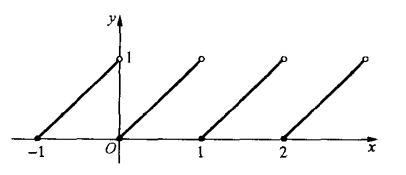
\includegraphics[width=\textwidth]{1.1.png} % 无需重复指定宽度  
\end{myimagebox}     
\caption{\label{fig:1.1}函数的图象}   
\end{figure}

接下来我们介绍\textbf{\color{btex}狄利克雷函数}。它的表达式如下:
\begin{align*}
    D(x)=\begin{cases}
        1 & x\text{是无理数}\\
        0 & x\text{是无理数}
    \end{cases}
\end{align*}

接下来我们介绍反函数的概念。若函数$f: X\to Y$是一个单射也是一个满射,那么逆映射$f^{-1}: X\to Y$就是一个反函数。\textbf{\color{btex}注意反函数的定义域和值域问题}。函数可以是有界的,如果$\forall x\in X$都有$f(x)\leq M$,称$M$是函数的上界。反之我们可以定义下界。\textbf{\color{btex}有界函数同时具有上界和下界。}(注意符号$\forall,\exists$分别表示任意,存在)。

\subsubsection{基本不等式和数学证明方法}
在高数的正式展开前,我们需要掌握一些基本的不等式。第一个不等式称作\textbf{\color{btex}Bernoulli伯努利不等式}:
\begin{tcolorbox}[
    colback=bac1,     % 极浅黄色背景
    colframe=fra1,   % 浅黄色边框
    coltitle=white,             % 标题文字白色
    coltext=tex1,
    title=Bernoulli不等式,
    fonttitle=\bfseries,        % 标题加粗
arc=3mm,                     % 圆角稍大
breakable
]
设$h>-1,n\in N^+$,那么下面不等式成立:
\begin{align*}
    (1+h)^n\geq 1+nh\tag{1-1}
\end{align*}

当$n>1$时,等号成立的充要条件为$h=0$。
\end{tcolorbox}

这个不等式的证明过程如下:
\begin{align*}
    (1+h)^n-1=h\cdot \sum_{k=1}^n (1+h)^{k-1}
\end{align*}

$\sum,\prod$分别代表连加和连乘。上面的式子右侧是等比数列,因此能说明这个式子成立。接下来我们进行分类讨论。当$h>0$,右侧连加重从第二项开始都大于1,因此$(1+h)^n-1\geq nh$。当$-1<h<0$时,右侧连加从第二项开始都小于1,因此连加和小于$n$,由于$h<0$,因此还能证明成立。

一般情况下,如果括号里是$(A+B)^n$,我们通常会做如下变换:
\begin{align*}
    (A+B)^n=A^n(1+\frac{B}{A})^n\geq A^n+nA^{n-1}B\tag{1-2}
\end{align*}

接下来我们讲述平均值不等式。在高中我们学到过这样的不等式($a,b>0$):
\begin{align*}
    \sqrt{ab}\leq \frac{1}{2}(a+b)\qquad a^2+b^2\geq 2ab
\end{align*}

接下来我们需要拓展一下此结论,介绍算术平均值-几何平均值不等式。
\begin{tcolorbox}[
    colback=bac1,     % 极浅黄色背景
    colframe=fra1,   % 浅黄色边框
    coltitle=white,             % 标题文字白色
    coltext=tex1,
    title=算术平均值——几何平均值不等式,
    fonttitle=\bfseries,        % 标题加粗
arc=3mm,                     % 圆角稍大
breakable
]
设$a_1,a_2,...a_n$都是非零实数,则下列不等式成立:
\begin{align*}
    \frac{a_1+a_2+...+a_n}{n}\geq \sqrt[n]{a_1a_2...a_n}\tag{1-3}
\end{align*}

\textbf{等号成立}的充要条件为$a_1=a_2=...=a_n$。
\end{tcolorbox}

这个证明需要使用\textbf{\color{btex}数学归纳法}。数学归纳法是先分析证明起点成立,在本题中,$n=2$的结论是我们的证明起点。接下来我们需要说明$n$处成立。那么这个问题可以转换成,如果我们假设$n=k$时结论成立,并利用这个条件去证明$n=k+1$时结论成立。那么我们就能证明原不等式成立了。假设1-3在$n=k$时成立,当$n=k+1$时,等式左侧可以写作:
\begin{align*}
    \frac{a_1+a_2+...+a_{k+1}}{k+1}=\frac{a_1+a_2+...+a_k}{k}+\frac{ka_{k+1}-a_1-a_2-...-a_k}{k(k+1)}
\end{align*}

将我们这个式子右边两项记为$A,B$,且$A,B>0$。那么根据式子1-2有:
\begin{align*}
    \left(\frac{a_1+a_2+...+a_{k+1}}{k+1}\right)^{k+1}&=(A+B)^{k+1}\geq A^{k+1}+(k+1)A^kB\\
    &=A^k[A+(k+1)B]\\
    &=\left(\frac{a_1+a_2+...+a_k}{k}\right)^{k}\cdot a_{k+1}\\
    &\geq a_1a_2...a_{k+1}
\end{align*}

因此结论在$n=k+1$也成立。根据数学归纳法1-3成立。等号成立的条件也可以使用数学归纳法证明,请读者自行完成。

接下来的不等式称作\textbf{\color{btex}绝对值不等式},也称三点不等式。其内容如下:
\begin{tcolorbox}[
    colback=bac2,     % 极浅黄色背景
    colframe=fra2,   % 浅黄色边框
    coltitle=white,             % 标题文字白色
    coltext=tex2,
    title=绝对值不等式,
    fonttitle=\bfseries,        % 标题加粗
arc=3mm,                     % 圆角稍大
breakable
]

若$a,b$都是实数,则下面不等式成立:
\begin{align*}
    |a|+|b|\geq |a+b|\tag{1-4}
\end{align*}

\textbf{等号成立}的条件是$a,b$两个实数同号。
\end{tcolorbox}

接下来我们介绍\textbf{\color{btex}Cauchy柯西不等式}。这个不等式有非常重要的应用:
\begin{tcolorbox}[
    colback=bac1,     % 极浅黄色背景
    colframe=fra1,   % 浅黄色边框
    coltitle=white,             % 标题文字白色
    coltext=tex1,
    title=Cauchy柯西不等式,
    fonttitle=\bfseries,        % 标题加粗
arc=3mm,                     % 圆角稍大
breakable
]
对于正实数$a_1,a_2,...a_n$和实数$b_1,b_2,...b_n$满足:
\begin{align*}
    \left|\sum_{i=1}^n a_ib_i\right|\leq \sqrt{\sum_{i=1}^n a_i^2}\sqrt{\sum_{i=1}^n b_i^2}\tag{1-5}
\end{align*}

\textbf{等号成立}的条件为$\frac{a_1}{b_1}=\frac{a_2}{b_2}=...=\frac{a_n}{b_n}$。
\end{tcolorbox}
在这里取等条件请读者完成。我们只证明这个不等式成立:我们引进一个变量$\lambda$,则有下面的式子成立:
\begin{align*}
    0\leq \sum_{i=1}^n(\lambda a_i-b_i)^2=\lambda^2\sum_{i=1}^n a_i^2-2\lambda\sum_{i=1}^n a_ib_i
+\sum_{i=1}^n b_i^2
\end{align*}

若$a_1=a_2=...=a_n=0$,那么Cauchy不等式已经成立。如果不是这种情况,上面的式子是一个关于$\lambda$的二次式,因此判别式$\Delta\geq 0$,即:
\begin{align*}
   \left(\sum_{i=1}^n a_ib_i\right)^2\leq\left(\sum_{i=1}^n a_i^2\right)\cdot
\left(\sum_{i=1}^n b_i^2\right)
\end{align*}

两边开方即可。接下来我们最后介绍一个关于三角函数的基本不等式:
\begin{tcolorbox}[
    colback=bac1,     % 极浅黄色背景
    colframe=fra1,   % 浅黄色边框
    coltitle=white,             % 标题文字白色
    coltext=tex1,
    title=三角函数基本不等式,
    fonttitle=\bfseries,        % 标题加粗
arc=3mm,                     % 圆角稍大
breakable
]
若$0<x<\frac{\pi}{2}$,则下面的基本不等式成立:
\begin{align*}
    \frac{2x}{\pi}<\sin x<x<\tan x\tag{1-6}
\end{align*}
\end{tcolorbox}

之前我们介绍了数学归纳法,其证明思路就是像多米诺骨牌一样一层层推进。接下来我们介绍\textbf{\color{btex}反证法},其核心思路是假设结论不正确,进一步推出和题目要求矛盾的结论。

\textbf{\color{btex}例}:证明$\sqrt{3}$不是有理数。

\textbf{\color{btex}解}:假设它是有理数,那么就存在两个互质正整数$m,n$使得:
\begin{align*}
    \sqrt{3}=\frac{m}{n}\to m^2=3n^2
\end{align*}

这就说明$m^2$是3的倍数,也就是说$m$是3的倍数。那么这反而说明$n^2$是3的倍数。因此$n$至少是3的倍数,与题设$m,n$互质的条件矛盾!

\subsubsection{序列极限}
设$\{a_n\}$是一个给定的序列,那么在$n$趋近于无穷大时,$a_n$的变化是什么情况呢?对于序列$a_n=\frac{1}{2^n}$,可以发行序列趋近于0;对于序列$a_n=\frac{1+(-1)^n}{n}$,虽然序列在震荡,但是也是趋近于0;对于序列$a_n=\sin\frac{n\pi}{2}$,它并没有一个趋近的数。因此我们需要用严格的序列极限的定义去阐述这种性质:
\begin{tcolorbox}[
    colback=bac2,     % 极浅黄色背景
    colframe=fra2,   % 浅黄色边框
    coltitle=white,             % 标题文字白色
    coltext=tex2,
    title=序列极限的定义,
    fonttitle=\bfseries,        % 标题加粗
arc=3mm,                     % 圆角稍大
breakable
]
设$\{a_n\}$是一个给定的序列,若存在常数$l$,对于\textbf{\color{btex}任意的正数}$\varepsilon$,无论它多么小\textbf{\color{btex}都存在一个正整数}$N$,使得\textbf{\color{btex}对任意}的$n>N$都有$|a_n-l|<\varepsilon$,那么我们称$l$是\textbf{\color{btex}序列极限},记作$\lim_{n\to\infty}a_n=l$。如果序列存在$l$,称该序列的极限存在。
\end{tcolorbox}

这种定义我们需要注意两个问题,第一,这是序列极限定义的$\varepsilon\sim N$说法,我们可以理解$\varepsilon$是“误差”,在序列项足够靠后的时候,所有的项都在误差范围之内。因此这个$N$是和$\varepsilon$有关的,因为精度越大误差越小时,序列满足的子列越要靠后。第二,如果我们用图象说明,就可以参考图1.2,更直观地说明$N-\varepsilon$语言的含义。
\begin{figure}[H]    
\centering     
\renewcommand{\figurename}{图}     
\renewcommand{\thefigure}{1.2}    
\begin{myimagebox}[width=0.45\textwidth] % 直接传入图片尺寸参数      
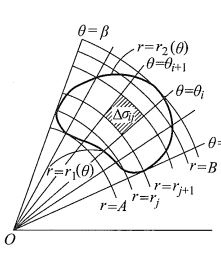
\includegraphics[width=\textwidth]{1.2.png} % 无需重复指定宽度  
\end{myimagebox}     
\caption{\label{fig:1.2}序列极限}   
\end{figure}

\textbf{\color{btex}例}:证明下面的极限成立。
\begin{align*}
   (1)\lim_{n\to \infty}\frac{1}{n^\alpha}=0 (\alpha>0) \qquad(2)\lim_{n\to\infty}\sqrt[n]{a}=1(a>1)\qquad (3)\lim_{n\to\infty}\frac{n^2+3n+10}{3n^2-n+2}=\frac{1}{3} 
\end{align*}

\textbf{\color{btex}解}:前两题是非常易得且需要记住的结论。我们利用序列极限的定义证明。对于第一题,我们的目标是对于$\forall \varepsilon>0$,可以找到一个$N_\varepsilon$,对于$\forall n>N_\varepsilon$都有:
\begin{align*}
    &|\frac{1}{n^\alpha}-0|<\varepsilon\to n^\alpha>\frac{1}{\varepsilon}\\
    & n>\sqrt[n]{\varepsilon^{-1}}
\end{align*}

也就是说,只要$n>\sqrt[n]{\varepsilon^{-1}}$就可以满足我们的要求。而我们现在是希望找到$n>N_\varepsilon$满足要求,因此$N_\varepsilon$一定要大于$\sqrt[n]{\varepsilon^{-1}}$。因此我们去取$\sqrt[n]{\varepsilon^{-1}}$向下取整再加1的数字即可。即就是$N_\varepsilon=[\sqrt[n]{\varepsilon^{-1}}+1]$。

对于第二题,我们继续找下面的式子满足时,$n$的要求:
\begin{align*}
    |\sqrt[n]{a}-1|<\varepsilon\to  a^{\frac{1}{n}}<1+\varepsilon
\end{align*}

两边取对数,则有:
\begin{align*}
    \frac{1}{n}\ln a<\ln(1+\varepsilon)\to n>\frac{\ln a}{\ln(1+\varepsilon)}
\end{align*}

因此我们取$N_\varepsilon=[\frac{\ln a}{\ln(1+\varepsilon)}]+1$。

第三个式子其实在说明,当$n\to\infty$时,\textbf{\color{btex}两个同阶次多项式除法的极限就是最高次系数的比值。}利用序列极限的定义去计算:
\begin{align*}
    \left|\frac{n^2+3n+10}{3n^2-n+2}-\frac{1}{3}\right|<\varepsilon\to \frac{\frac{10}{3}n+\frac{28}{3}}{3n^2-n+2}<\varepsilon    
\end{align*}

如果我们可以把不等式左侧适当放大,那么$N_\varepsilon$的要求会更严苛,那么如果我们找到这个$N_\varepsilon$也可以,也就是说如果$a<b<\varepsilon$,那么$b<\varepsilon$的那个$N_\varepsilon$一定也可以满足$a<\varepsilon$,因此:
\begin{align*}
    \frac{\frac{10}{3}n+\frac{28}{3}}{3n^2-n+2}=\frac{10n+28}{3[2n^2+n(n-1)+2]}<\frac{10n+10n}{3\cdot 2n^2}=\frac{10}{3n}
\end{align*}

注意第二个小于号是在$n$足够大的时候($n>3$)才可以成立。因此本题中,$n$足够大时,我们的$a<b<\varepsilon$即就是:
\begin{align*}
     \frac{\frac{10}{3}n+\frac{28}{3}}{3n^2-n+2}<\frac{10}{3n}<\varepsilon\to n>\frac{10}{3\varepsilon}
\end{align*}

因此如果$n>3$并且$n>\frac{10}{3\varepsilon}$时,就能满足条件。而$n>N_\varepsilon$应该同时满足二者条件。因此$N_\varepsilon$应该是二者最大的那一项取整加1,因此:
\begin{align*}
    N_\varepsilon=[\max\{3,\frac{10}{3\varepsilon}\}]+1
\end{align*}

当然,简单的序列极限可以直接用定义证明,有些极限比较复杂。因此需要新的办法,接下来我们来介绍夹逼定理:
\begin{tcolorbox}[
    colback=bac2,     % 极浅黄色背景
    colframe=fra2,   % 浅黄色边框
    coltitle=white,             % 标题文字白色
    coltext=tex2,
    title=夹逼定理,
    fonttitle=\bfseries,        % 标题加粗
arc=3mm,                     % 圆角稍大
breakable
]

设三个序列$\{a_n\},\{b_n\},\{c_n\}$,且存在一个正整数$N_0$使得$\forall n \geq N_0$都有:
\begin{align*}
    c_n\leq a_n\leq b_n
\end{align*}

且$\lim_{n\to\infty}c_n=\lim_{n\to\infty}b_n=l,\{a_n\}$序列存在极限,则$\lim_{n\to\infty}a_n=l$
\end{tcolorbox}

接下来我们进行定理证明。根据极限的定义,有:
\begin{align*}
 |b_n-l|<\varepsilon,\forall n>N_1\qquad |c_n-l|<\varepsilon,\forall n>N_2 
\end{align*}

那么就有当$\forall n>N=\max\{N_0,N_1,N_2\}$有:
\begin{align*}
    l-\varepsilon <c_n\leq a_n\leq b_n<l+\varepsilon
\end{align*}

即就有:
\begin{align*}
    |a_n-l|<\varepsilon ,\forall n>N
\end{align*}

\textbf{\color{btex}例}:利用夹逼定理计算极限:
\begin{align*}
 & (1) \lim_{n\to\infty}\frac{a^n}{n!}\;(a>1) \qquad (2)\lim_{n\to\infty}\frac{n^{k-1}}{(n-1)(n-2)...(n-k)}(k>1,k\in\mathbb{N^+})\\
&(3) \lim_{n\to\infty} \frac{n^k}{a^n}=0 (k\in\mathbb{N^+},a>1)  
\end{align*}

\textbf{\color{btex}解}:第一问的极限是想说明,\textbf{\color{btex}阶乘比指数增长速度更快}。我们考虑$n>[a]+1$,有:
\begin{align*}
  b_n=  0\leq a_n=\frac{a^{[a]}}{[a]!}\cdot\frac{a}{[a]+1}\cdot ...\cdot \frac{a}{n}<\frac{a^{[a]}}{[a]!}\cdot \frac{a}{n}=c_n
\end{align*}

当$n\to\infty$时,$c_n\to 0$,而$b_n=0$,因此原极限为0。

第二问,我们设原式子为$a_n$,分子和分母同除$n^k$有:
\begin{align*}
    b_n=0\leq a_n=\frac{\frac{1}{n}}{(1-\frac{1}{n})(1-\frac{2}{n})...(1-\frac{k}{n})}=c_n
\end{align*}

当$n$足够大时,$n>2k$,则$c_n\leq\frac{2^k}{n}=d_n$,而$d_n$极限为0,证毕。

对于第三问,我们先令$a=1+h$,那么根据二项式定理:
\begin{tcolorbox}[
    colback=bac1,     % 极浅黄色背景
    colframe=fra1,   % 浅黄色边框
    coltitle=white,             % 标题文字白色
    coltext=tex1,
    title=二项式定理,
    fonttitle=\bfseries,        % 标题加粗
arc=3mm,                     % 圆角稍大
breakable
]
设$n$为整数,则:
\begin{align*}
    (a+b)^n=\sum_{k=0}^n C_{n}^k a^kb^{n-k}\tag{1-7}
\end{align*}
\end{tcolorbox}
\begin{align*}
a^n&=(1+h)^n=1+nh+\frac{n(n-1)}{2!}h^2+...+\frac{n(n-1)...(n-k)}{(k+1)!} h^{k+1}+...+h^n\\
 &\geq \frac{n(n-1)...(n-k)}{(k+1)!} h^{k+1} \;(n>1) 
\end{align*}

因此:
\begin{align*}
    b_n=0\leq a_n\leq c_n=n^k \cdot \frac{(k+1)!}{n(n-1)..(n-k)h^{n+1}}
\end{align*}

根据第二问的结论,$\lim_{n\to\infty} c_n=0$,因此原式极限为0。注意这里我们把幂次利用二项式定理进行放缩。

极限之间也有不等式和四则运算。我们来介绍一些定理:
\begin{tcolorbox}[
    colback=bac2,     % 极浅黄色背景
    colframe=fra2,   % 浅黄色边框
    coltitle=white,             % 标题文字白色
    coltext=tex2,
    title=极限不等式,
    fonttitle=\bfseries,        % 标题加粗
arc=3mm,                     % 圆角稍大
breakable
]
若$\lim_{n\to\infty}a_n=l_1,\lim_{n\to\infty}b_n=l_2,l_1<l_2,$则$\exists N\in \mathbb{N^+}$,使得$\forall n>N,a_n<b_n$
\end{tcolorbox}

这个定理的证明思路是核心。我们先利用极限的定义,得到在$n$足够大时,序列在一定误差范围内摆动,进一步:
\begin{align*}
    a_n<l_1+\varepsilon,b_n>l_2-\varepsilon,\forall N>\max\{N_1,N_2\}
\end{align*}

由于这个$\varepsilon$是任取的,因此我们取$\varepsilon$满足$l_1+\varepsilon<l_2-\varepsilon$即可。

它的逆定理也是需要注意的。设序列$\lim_{n\to\infty}a_n=l_1,\lim_{n\to\infty}b_n=l_2$,并且存在正整数$N$使得$\forall n>N,a_n\geq b_n$,则$l_1\geq l_2$。注意即使$a_n$严格大于$b_n$,二者极限也可能一致。

极限满足加减乘除的四则运算。我们在这里给出乘法的证明过程作为参考。(加减法比较简单,直接代入绝对值不等式即可证明)。

假设$\lim_{n\to\infty}a_n=l_1,\lim_{n\to\infty}b_n=l_2$,我们要证明在$n$足够大时$|a_nb_n-l_1l_2|<\varepsilon$,因此我们可以把等式左侧适当放大,让放大后的结果小于$\varepsilon$:
\begin{align*}
    |a_nb_n-l_1l_2|=&|(a_n-l_1)b_n+l_1(b_n-l_2)|\leq |b_n(a_n-l_1)|+|l_1(b_n-l_2)|\\
    \leq&|b_n||a_n-l_1|+|l_1||b_n-l_2|
\end{align*}

由于$b_n\to l_2$,我们选择误差为1,也就是说$|b_n-l_2|<1$,此时这个不等式可以在$n>N_b$成立。因此把上面的不等式利用绝对值不等式变形可以得到:
\begin{align*}
    |b_n|<1+|l_2|\qquad \forall n>N_b
\end{align*}

因此不等式右侧可以继续放大,可以得到:
\begin{align*}
   |b_n||a_n-l_1|+|l_1||b_n-l_2|<(1+|l_2|)|a_n-l_1|+|l_1||b_n-l_2|
\end{align*}

如果不等式右侧小于$\varepsilon$就可以了。接下来由于$a_n\to l_1$,我们令误差范围为$\varepsilon'=\frac{\varepsilon}{2(1+|l_2|)}$,那么对于$n>N_2$,就有:
\begin{align*}
    |a_n-l_1|<\frac{\varepsilon}{2(1+|l_2|)}
\end{align*}

进一步对于$\varepsilon''=\frac{\varepsilon}{2(1+|l_1|)}$,也有:
\begin{align*}
    |b_n-l_2|<\frac{\varepsilon}{2(1+|l_1|)}
\end{align*}

代入到上面的不等式证毕。这个定理的证明可以帮助更好理解极限的含义以及极限定义的灵活运用。

\textbf{\color{btex}例}:计算下列极限
\begin{align*}
(1)\lim_{n\to\infty}\frac{n^3+5n+1}{4n^3+8} \qquad (2) \lim_{n\to\infty} (\sqrt{n+\sqrt{n}}-\sqrt{n} )
\end{align*}

\textbf{\color{btex}解}:对于第一问我们不能直接计算分子和分母的极限。因为不存在。因此分子分母同除$n^3$则有:
\begin{align*}
\lim_{n\to\infty}\frac{n^3+5n+1}{4n^3+8}=\frac{\lim_{n\to\infty}(1+\frac{5}{n^2}+\frac{1}{n^3})}
{\lim_{n\to\infty}(4+\frac{8}{n^3})}=\frac{1}{4} 
\end{align*}

对于第二问,我们使用\textbf{\color{btex}分子有理化}。所以我们做下面的变形:
\begin{align*}
    \sqrt{n+\sqrt{n}}-\sqrt{n}=\frac{\sqrt{n}}{\sqrt{n+\sqrt{n}}+\sqrt{n}}=\frac{1}{\sqrt{1+\frac{1}{n}}+1}\to \frac{1}{2}
\end{align*}

接下来我们继续讲一个定理:\textbf{\color{btex}有极限的序列,其子列必有相同的极限}。这个定理很好证明,不过它给我们提供一种证明序列不存在极限的方式:\textbf{\color{btex}找序列的两个子列,它们有不同的极限}。

接下来我们介绍一个重要极限:
\begin{tcolorbox}[
    colback=bac1,     % 极浅黄色背景
    colframe=fra1,   % 浅黄色边框
    coltitle=white,             % 标题文字白色
    coltext=tex1,
    title=自然对数极限,
    fonttitle=\bfseries,        % 标题加粗
arc=3mm,                     % 圆角稍大
breakable
]
当$n\to\infty$时,有:
\begin{align*}
    \lim_{n\to\infty}(1+\frac{1}{n})^n=e\tag{1-8}
\end{align*}
\end{tcolorbox}

在分析这个定理前,我们先去介绍,这个极限等于$e$是规定的。因此你用自然对数去证明极限为$e$属于是儿子证爸爸的关系。因此我们需要证明这个极限存在,$e\approx 2.718$。另一方面为了证明极限存在,我们需要说明:\textbf{\color{btex}单调递增有上界的序列一定有极限,单调递减有下界的序列一定有极限。}这个定理我们不进行过多证明,其正确性是显然的。首先我们证明它是单调递增的,因为根据二项式定理有:
\begin{align*}
&(1+\frac{1}{n})^n=1+1+\sum_{k=2}^n\frac{1}{k!}(1-\frac{1}{n})...(1-\frac{k-1}{n})\\
 &(1+\frac{1}{n+1})^{n+1}=1+1+\sum_{k=2}^n\frac{1}{k!}(1-\frac{1}{n+1})...(1-\frac{k-1}{n+1})+
(\frac{1}{n+1})^{n+1}     
\end{align*}

把这两个式子进行比较,就可以得到:
\begin{align*}
   (1+\frac{1}{n})^n<(1+\frac{1}{n+1})^{n+1} 
\end{align*}

单调递增性证毕。接下来我们需要证明原极限有上限。我们利用二项式定理进行放缩:
\begin{align*}
(1+\frac{1}{n})^n&=1+\sum_{i=1}^n C_{n}^i\frac{1}{n^i}<1+1+\frac{1}{2!}+...+\frac{1}{n!}\\
& <1+1+\frac{1}{1\cdot 2}+...+\frac{1}{(n-1)n} \\
&=1+1+1-\frac{1}{n}<3    
\end{align*}

因此原序列存在上界。因此原极限存在。接下来我们再介绍一个极限:
\begin{tcolorbox}[
    colback=bac1,     % 极浅黄色背景
    colframe=fra1,   % 浅黄色边框
    coltitle=white,             % 标题文字白色
    coltext=tex1,
    title=Euler常数,
    fonttitle=\bfseries,        % 标题加粗
arc=3mm,                     % 圆角稍大
breakable
]
证明下面的序列存在极限:
\begin{align*}
    c_n=1+\frac{1}{2}+...+\frac{1}{n}-\ln n\to \gamma\tag{1-9}
\end{align*}

这个序列的极限定义为\textbf{\color{btex}Euler常数}$\gamma\approx 0.577$
\end{tcolorbox}

我们先证明数列是单调递减的。我们用后一项减去前一项,得到:
\begin{align*}
    c_{n+1}-c_n=\frac{1}{n+1}-\ln (n+1)+\ln n=\frac{1}{n+1}-\ln(1+\frac{1}{n})<0
\end{align*}

接下来证明数列有下界。由于$\ln(1+\frac{1}{n})>\frac{1}{n}$,则有:
\begin{align*}
    c_n>\ln\frac{2}{1}+\ln\frac{3}{2}+...+\ln\frac{n+1}{n}-\ln n=\ln\frac{n+1}{n}>0
\end{align*}

因此原序列存在极限。

\subsection{函数极限与应用}
\subsubsection{函数极限}
函数极限和序列极限不同。函数极限的自变量$x$时任意的。并且我们考虑函数在$x_0$附近的极限情况时,要从左趋近和右趋近两种情况进行分析。我们对一些符号进行规定。左趋近记成$x\to a+0$,右趋近记作$x\to a-0$,同时从两侧趋近记作$x\to a$,趋近于无穷大或者负无穷大为$x\to\infty,x\to -\infty$。我们考虑函数$f(x)=\sin\frac{1}{x}$和函数$f(x)=x\sin \frac{1}{x}$两种情况。我们发现,前者在0处,无论是左趋近还是右趋近是没有极限的,而后者是有的。
\begin{figure}[H]    
\centering     
\renewcommand{\figurename}{图}     
\renewcommand{\thefigure}{1.3}    
\begin{myimagebox}[width=0.4\textwidth] % 直接传入图片尺寸参数      
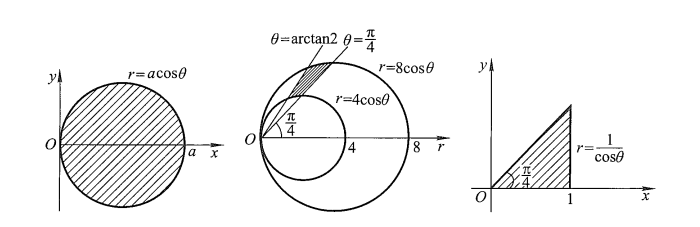
\includegraphics[width=\textwidth]{1.3.png} % 无需重复指定宽度  
\end{myimagebox}     
\caption{\label{fig:1.3}$f(x)=\sin\frac{1}{x}$}   
\end{figure}
\begin{figure}[H]    
\centering     
\renewcommand{\figurename}{图}     
\renewcommand{\thefigure}{1.4}    
\begin{myimagebox}[width=0.4\textwidth] % 直接传入图片尺寸参数      
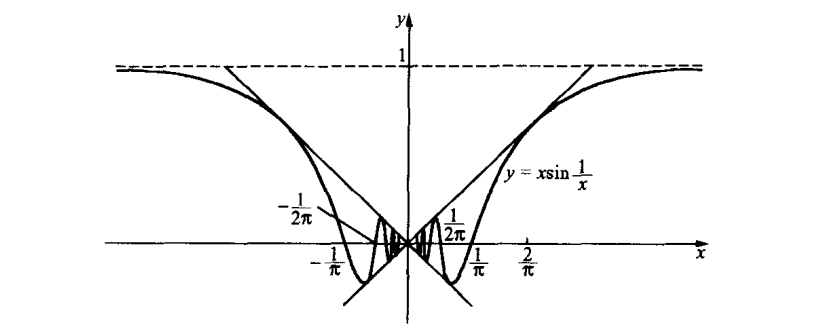
\includegraphics[width=\textwidth]{1.4.png} % 无需重复指定宽度  
\end{myimagebox}     
\caption{\label{fig:1.4}$f(x)=x\sin\frac{1}{x}$}   
\end{figure}

为什么我们要区分左极限和右极限呢?因为对于符号函数,我们发现如果不在0处,那么对于$a$附近,从左侧趋近和从右侧趋近的极限是一样的。但是在0处,左趋近是$-1$,右趋近是$1$,因此它们是有区别的。因此我们有必要去定义单侧极限。我们可以类比序列极限的定义去定义函数单侧极限:
\begin{tcolorbox}[
    colback=bac2,     % 极浅黄色背景
    colframe=fra2,   % 浅黄色边框
    coltitle=white,             % 标题文字白色
    coltext=tex2,
    title=函数单侧极限,
    fonttitle=\bfseries,        % 标题加粗
arc=3mm,                     % 圆角稍大
breakable
]
设函数$y=f(x)$的定义域为$(a,b)$,若存在一个常数$l$,对任意的$\varepsilon>0$,无论它多么小,都存在一个$\delta>0$,使得$\forall x\in(a,a+\delta)$都有$|f(x)-l|<\varepsilon$,则称作当$x\to a+0$时,函数的\textbf{\color{btex}右极限}为$l$,记作$\lim_{x\to a+0}f(x)=l$。同理我们定义左极限。
\end{tcolorbox}

从几何上讲,单侧极限的定义非常简单。也就是说对于一个任意的误差范围$\varepsilon$,都能在点$a$右侧找到一个区域,使得区域上的所有点函数值都在误差范围之内。接下来我们定义函数的双侧极限:
\begin{tcolorbox}[
    colback=bac2,     % 极浅黄色背景
    colframe=fra2,   % 浅黄色边框
    coltitle=white,             % 标题文字白色
    coltext=tex2,
    title=函数双侧极限,
    fonttitle=\bfseries,        % 标题加粗
arc=3mm,                     % 圆角稍大
breakable
]
设函数$y=f(x)$的定义域为在点$a$的空心邻域$(a-r,a)\cup (a,a+r)$(在点$a$处不必有定义),若存在常数$l$,对于任意小的$\varepsilon$,都存在一个$\delta$,使得$\forall x\in (a-\delta,a+\delta)$都有$|f(x)-l|<\varepsilon$,称$l$是函数在$a$处的\textbf{\color{btex}双侧极限}(简称极限),记作$\lim_{x\to a}f(x)=l$
\end{tcolorbox}

例如符号函数在$0$处存在左极限和有极限,但是在$0$自己这一点却没有双侧极限。\textbf{\color{btex}函数极限也有极限四则运算,极限夹逼定理,极限不等式。并且上一章我们讲述了序列极限证明不存在的办法。对于函数极限同理,也是找两个子列,它们的极限不同。这一部分不再赘述,书上都有相关解释。}

\textbf{\color{btex}例}:计算前三个函数极限成立,并证明第四个函数极限不存在
\begin{align*}
(1) \lim_{x\to a}\sin x=\sin a\quad (2)\lim_{x\to 0}\frac{\sin x}{x}=1\quad (3)\lim_{x\to \infty}(1+\frac{1}{x})^x=e  \quad (4)\lim_{x\to 0}\sin\frac{1}{x}
\end{align*}

\textbf{\color{btex}解}:对于第一个极限我们使用$N\sim\varepsilon$语言,由于:
\begin{align*}
    |\sin x-\sin a|=|2\sin \frac{x-a}{2}\cos\frac{x+a}{2}|\leq 2|\sin \frac{x-a|}{2}|\leq|x-a|
\end{align*}

因此只要$|x-a|<\varepsilon$,原差值也一定小于$\varepsilon$,不妨取$\delta=\varepsilon$即可。\textbf{\color{btex}第二问的极限是一个非常重要的结论}。由于三角不等式$\sin x<x<\tan x$,因此可以得到$\cos x<\frac{\sin x}{x}<1$,利用夹逼定理得证。第三问我们要注意,在函数极限中$x\to\infty$是同时趋向正无穷和负无穷的。我们先看正无穷的情况:记$n=[x]$,则有:
\begin{align*}
    (1+\frac{1}{n+1})^n\leq (1+\frac{1}{x})^x\leq (1+\frac{1}{n})^{n+1}
\end{align*}

可以证明不等式左侧和右侧的极限都是$e$,根据夹逼定理,原极限为$e$。对于负无穷的情况,做换元$y=-x$,原极限可写作:
\begin{align*}
    \lim_{x\to -\infty}(1+\frac{1}{x})^x=\lim_{y\to \infty}(1-\frac{1}{y})^{-y}=\lim_{y\to \infty}(1+\frac{1}{y-1})^{y}=e
\end{align*}

最后我们介绍无穷小量和无穷大量的概念,这个概念对于我们计算极限也有作用。我们先介绍无穷大量:
\begin{tcolorbox}[
    colback=bac2,     % 极浅黄色背景
    colframe=fra2,   % 浅黄色边框
    coltitle=white,             % 标题文字白色
    coltext=tex2,
    title=无穷大量,
    fonttitle=\bfseries,        % 标题加粗
arc=3mm,                     % 圆角稍大
breakable
]
设函数$f(x)$在$x_0$的空心邻域内有定义,若对于任意的正数$M$,无论它多么大都存在一个$\delta>0$,使得当$0<|x-x_0|<\delta$时都有$|f(x)|>M$,则称$x\to x_0$时$f(x)$为无穷大量,记作$\lim_{x\to x_0}f(x)=\infty$。四则运算对无穷大量不成立。
\end{tcolorbox}

无穷小量类似,是指以0为极限的变量。例如当$n\to\infty$时,$\frac{1}{n},\frac{1}{n!}$都是无穷小量。如果当$x\to a$时$f(x),g(x)$都是无穷小量,那么$f(x)g(x)$也是无穷小量。然而$\frac{f(x)}{g(x)}$不一定。如果$\lim_{x\to a}\frac{f(x)}{g(x)}\to 1$,我们称二者是\textbf{\color{btex}等价无穷小},记作$f(x)\sim g(x)$。例如$x\to 0$时,$\sin x\sim x\sim \tan x,\ln(1+x)\sim x$,$1-\cos x\sim \frac{1}{2}x^2,(1+x)^\alpha\sim \alpha x$。我们只对最后一个式子进行证明,我们记记$u=(1+x)^\alpha-1$则有:
\begin{align*}
    \frac{(1+x)^\alpha-1}{\alpha x}=\frac{(1+x)^\alpha-1}{\alpha \ln(1+x)}\cdot\frac{\alpha\ln(1+x)}{\alpha x}=\frac{u}{\ln(1+u)}\cdot\frac{\ln(1+x)}{x}\to 1 ({u\to 0,x\to 0})
\end{align*}

无穷小趋近于0的速度也不同,当一个无穷小量$\alpha(x)$比另一个无穷小量$\beta(x)$趋近于0更快的时候,我们称$\alpha(x)$是\textbf{\color{btex}高阶无穷小量},记作$\alpha(x)=o(\beta(x))$。如果$\lim_{x\to a}\frac{f(x)}{g(x)}=l\neq 0$是一个不为0的常数,称它们是\textbf{\color{btex}同阶无穷小量}。如果$f(x)$与$(x-a)^n,x\to a$是同阶的,称$f(x)$是$n$阶无穷小量。

\textbf{\color{btex}例}:计算下列极限,并说明分子在$x\to 0$是几阶无穷小量。
\begin{align*}
    \lim_{x\to\infty}\frac{\tan 5x-\sin 3x}{2x}
\end{align*}

\textbf{\color{btex}解}:\textbf{\color{btex}无穷小量在极限中可以进行相互替代}。当$x\to 0,\sin x\sim x\sim \tan x$(\textbf{但一定要注意,等价无穷小替换中$x$是存在先决条件的}),因此:
\begin{align*}
    \lim_{x\to\infty}\frac{\tan 5x-\sin 3x}{2x}=\lim_{x\to\infty}\frac{5x-3x}{2x}=1
\end{align*}

根据极限的答案,分子是一阶无穷小量。然而无穷小量直接替代法有时不能直接使用,例如计算:
\begin{align*}
    \lim_{x\to\infty}\frac{\tan x-\sin x}{x^3}
\end{align*}

这里不能把分子做直接无穷小量替换,答案是0(实际上学了泰勒展开之后我们就可以有更深的理解)。因此我们要先做变形,然后用无穷小量替代法:
\begin{align*}
    \lim_{x\to\infty}\frac{\tan x-\sin x}{x^3}=\lim_{x\to\infty}\frac{\tan x}{x}\frac{(1-\cos x)}{x^2}=\frac{1}{2}
\end{align*}

分子此时是一个3阶无穷小量。最后我们介绍一个定理,$f(x)\sim g(x)$的充要条件是$f(x)=g(x)+o(f(x))$。这个定理直接用等价无穷小的定义证明即可。

\subsubsection{连续函数}
在初中,我们接触的函数大多都是连续函数。那么一个函数的连续性怎么严格定义?从图形上说,连续代表着“不间断”,我们用数学语言对连续性进行严谨证明:
\begin{tcolorbox}[
    colback=bac2,     % 极浅黄色背景
    colframe=fra2,   % 浅黄色边框
    coltitle=white,             % 标题文字白色
    coltext=tex2,
    title=连续的定义,
    fonttitle=\bfseries,        % 标题加粗
arc=3mm,                     % 圆角稍大
breakable
]
若函数$f(x)$在区间$(a,b)$有定义,若$f(x)$在店$x_0\in(a,b)$有双侧极限并且等于函数值$f(x_0)$,那么称$y=f(x)$在$x_0$上连续。若$\forall x_0\in(a,b)$都满足上述条件,称函数在$(a,b)$连续。
\end{tcolorbox}

我们可以发现,初等函数都是连续的。函数$[x]$在所有整数点上不连续。狄利克雷函数处处不连续。当然对于上述关于连续性的描述也可以用如下的数学语言概括:
\begin{align*}
    \forall \varepsilon>0,\exists \delta >0\to \forall |x-x_0|<\delta\quad|f(x)-f(x_0)|<\varepsilon
\end{align*}

然而利用$N-\varepsilon$语言也通常难以说明函数的连续性。因此我们常用下边的\textbf{\color{btex}Lipschitz条件}证明连续性:
\begin{tcolorbox}[
    colback=bac1,     % 极浅黄色背景
    colframe=fra1,   % 浅黄色边框
    coltitle=white,             % 标题文字白色
    coltext=tex1,
    title=Lipschitz条件,
    fonttitle=\bfseries,        % 标题加粗
arc=3mm,                     % 圆角稍大
breakable
]
函数$f(x)$在$(a,b)$上连续的一个\textbf{\color{btex}充分不必要条件}为:
\begin{align*}
    |f(x_1)-f(x_2)|\leq L|x_1-x_2|,\forall x_1,x_2\in (a,b)
\end{align*}
\end{tcolorbox}

\textbf{\color{btex}例}:利用Lipschitz条件说明$\sin x$在实数域上连续,并且利用$\sqrt{x}$来说明Lips条件不是必要条件。

\textbf{\color{btex}解}:我们在实数域上任取$x_1,x_2$,有:
\begin{align*}
    |\sin x_1-\sin x_2|=2|\sin\frac{x_1-x_2}{2}\cos\frac{x_1+x_2}{2}|\leq 2|\sin\frac{x_1-x_2}{2}|\leq |x_1-x_2|
\end{align*}

取$L=1$即可。对于第二个例子,取$x_2=0$,则$|\sqrt{x_1}|\leq L x_1$找不到合适的$L$使得$\forall x_1\geq 0$都成立。然而$\sqrt{x}$在$x=0$处是连续的。

接下来我们介绍复合函数和反函数的连续性。证明过程这里不再赘述,读者可自行看书。
\begin{tcolorbox}[
    colback=bac2,     % 极浅黄色背景
    colframe=fra2,   % 浅黄色边框
    coltitle=white,             % 标题文字白色
    coltext=tex2,
    title=复合函数的连续性,
    fonttitle=\bfseries,        % 标题加粗
arc=3mm,                     % 圆角稍大
breakable
]
设函数$f:(a,b)\to (c,d)$在点$x_0$处连续,函数$g:(c,d)\to R$在点$f(x_0)$处连续,则复合函数$g(f(x))$在$x_0$处连续。进一步我们有:
\begin{align*}
    \lim_{x\to a}g(f(x))=g(\lim_{x\to a}f(x))
\end{align*}
\end{tcolorbox}

函数的单调性在高中已经有所接触,在这里我们补充“严格单调”和单调的区别。严格单调必须要严格大于或者严格小于。根据严格单调的定义我们介绍反函数的连续性:
\begin{tcolorbox}[
    colback=bac2,     % 极浅黄色背景
    colframe=fra2,   % 浅黄色边框
    coltitle=white,             % 标题文字白色
    coltext=tex2,
    title=反函数的连续性,
    fonttitle=\bfseries,        % 标题加粗
arc=3mm,                     % 圆角稍大
breakable
]
设函数$f: (a,b)\to (c,d)$是一个满射,并且是严格单调的函数。则$f$是$(a,b)$上的连续函数,$f^{-1}$是$(c,d)$的连续函数。
\end{tcolorbox}

接下来我们介绍间断点。函数在不连续处的点称作间断点。假设$x_0$是函数$y=f(x)$的一个间断点,那么有两种可能性。第一种$\lim_{x\to x_0+0}f(x)$与$\lim_{x\to x_0-0}f(x)$都存在,但\textbf{\color{btex}彼此不相等或者相等但不等于$f(x_0)$,称作函数的第一类间断点。}如果第一类间断点是彼此相等但不等于$f(x_0)$的情况,又可称作\textbf{\color{btex}可去间断点}。如果左极限和右极限至少一个不存在,称作\textbf{\color{btex}第二类间断点}。

\textbf{\color{btex}例}:指出下面分段函数的间断点和类型:
\begin{align*}
    f(x)=\begin{cases}
        \frac{\sin x}{x(1-x)}& x\neq 0,1\\
        -1&x=0\\
        1& x=1
    \end{cases}
\end{align*}

\textbf{\color{btex}解}:这个函数可能的间断点是0,1.首先我们开展0处的左极限和右极限,显然是相等的,因此0是一个可去间断点。
\begin{align*}
    \lim_{x\to\infty}\frac{\sin x}{x(1-x)}=\lim_{x\to 0}\frac{1}{1-x}=1
\end{align*}

在1处,由于$\lim_{x\to1+0}f(x)=-\infty$,因此1是第二类间断点。

闭区间上的连续函数有非常重要的性质,在这里我们只做介绍,其证明需要数学分析课程中的方法。这些定理在日后的学习非常重要:
\begin{tcolorbox}[
    colback=bac2,     % 极浅黄色背景
    colframe=fra2,   % 浅黄色边框
    coltitle=white,             % 标题文字白色
    coltext=tex2,
    title=闭区间连续函数的性质,
    fonttitle=\bfseries,        % 标题加粗
arc=3mm,                     % 圆角稍大
breakable
]
\textbf{\color{btex}定理1:介值定理}:设函数$f(x)\in[a,b]$是闭区间连续函数,且$f(a)\neq f(b)$,则对于任何一个在$f(a),f(b)$之间的值$\eta$,都能找到一点$\xi \in(a,b)$使得$f(\xi)=\eta$。

\textbf{\color{btex}定理2:最值定理}:设函数$f(x)\in[a,b]$是闭区间连续函数,那么函数有最大值和最小值。

\textbf{\color{btex}定理3:有界定理}:闭区间上连续函数有界。
\end{tcolorbox}

这些定理具有广泛的应用,我们看下面的两个例题:

\textbf{\color{btex}例}:(1)证明任意奇数次实系数多项式至少有一个实根。

(2)设函数$f(x)$在$[0,2]$上连续,并且$f(0)=f(2)$,证明在$[0,2]$有两点$x_1,x_2$使得:
\begin{align*}
    |x_1-x_2|=1\qquad f(x_1)=f(x_2)
\end{align*}

\textbf{\color{btex}解}:对于第一题,我们考虑这样的一个奇数次多项式:
\begin{align*}
    P(x)=a_0x^{2k+1}+a_1x^{2k}+...+a_{2k+1}=x^{2k+1}(a_0+\frac{a_1}{x}+...+\frac{a_{2k+1}}{x^{2k+1}})\qquad |x|>0
\end{align*}

当$x\to\infty$时,括号内部趋向于$a_0$,因此$P(x)$符号与$x^{2k+1}$一致。当$x\to+\infty$时,$P(x)\to+\infty$。当$x\to -\infty$时同理。因此根据极限定义,存在$x_1$使得$P(x_1)<0$,存在$x_2$使得$P(x_2)>0$。在闭区间上$[x_1,x_2]$上使用介值定理,原命题成立。

第二题的处理方式一致,我们可以去考虑构造函数$g(x)=f(x+1)-f(x)$,不妨令$x_1>x
_2$,因此原命题是去寻找$g(x)$存在零点。由于:
\begin{align*}
    g(0)=f(1)-f(0)=-g(1)
\end{align*}

如果说$g(0)=g(1)=0$,直接成立。如果$g(0)>0$,那么$g(1)<0$。根据介值定理$g(x)$在闭区间$[0,1]$上有零点。

我们最后介绍一个定理,若一个连续函数有单值反函数,其反函数必连续。
\subsection{习题补充与拓展}
本章的重点在于利用各种方法计算序列极限和函数极限,下面我们提供一些更深层次的例题加深理解。在今后我们说,序列$\{a_n\}$有极限和序列收敛的说法是一样的,若遇到不同表述请不必惊讶。

\textbf{\color{btex}例1}:计算下列序列极限:
\begin{align*}
&(1) \lim_{n\to\infty }\sqrt[n]{a_1^n+a_2^n+...+a_p^n}\;(0<a_1<...<a_p)\qquad 
(2)\lim_{n\to\infty}(1+x)(1+x^2)...(1+x^n),0<x<1\\
&(3)\lim_{n\to\infty}\sum_{k=1}^n\frac{1}{k(k+1)...(k+\alpha)}\;(\alpha\in  \mathbb{N^+})\qquad
(4)\lim_{n\to\infty}s_n\;(s_n=a+3a^2+...+(2n-1)a^n,|a|<1) 
\end{align*}

\textbf{\color{btex}解}:对于第一题,利用夹逼定理可以得到
\begin{align*}
    \sqrt[p]{a_p^n}<a_n<\sqrt[n]{pa_p^n}
\end{align*}

对两侧取极限,左侧和右侧的极限都为$a_p$,因此原序列极限为$a_p$。第二个例子中,我们利用\textbf{\color{btex}“滚雪球”}的办法,上下同时乘以$1-x$,因此:
\begin{align*}
    a_n=\frac{(1-x)(1+x)...(1+x^n)}{1-x}=\frac{1-x^{2n}}{1-x}\to\frac{1}{1-x}
\end{align*}

第三问\textbf{\color{btex}裂项法},由于:
\begin{align*}
    \sum_{k=1}^n\frac{1}{k(k+1)...(k+\alpha)}=\sum_{k=1}^n \left[\frac{1}{k(k+1)...(k+\alpha-1)}-\frac{1}{(k+1)(k+2)...(k+\alpha)}\right]\cdot\frac{1}{\alpha}
\end{align*}

因此裂项相加,原极限应该为:
\begin{align*}
\lim_{n\to\infty}\frac{1}{\alpha}\left[\frac{1}{\alpha!}-\frac{1}{(n+1)(n+2)...(n+\alpha)}\right]=\frac{1}{\alpha \alpha!}
\end{align*}

第四题是非常标准的错位相减法。我们计算$s_n-as_n$:
\begin{gather*}
    s_n-as_n=a+2a^2+2a^3+...+2a^n-(2n-1)a^{n+1}=2\frac{a(1-a^n)}{1-a}-a-(2n-1)a^{n+1}\\
    \lim_{n\to\infty}s_n=\frac{a(a+1)}{(a-1)^2}
\end{gather*}

\textbf{\color{btex}例2}:设$0<x_0<\frac{\pi}{2},x_n=\sin x_{n-1}$,试说明$\lim_{n\to\infty}x_n$存在并求值。

\textbf{\color{btex}解}:首先我们说明该序列单调递减。由于$x_{n-1}=\arcsin x_n<x_n$成立,因此单调递减确立。另一方面,$x_n>0$,因此序列单调递减有下界,极限存在。这是一个递推序列,当$n\to\infty$时,令极限为$a$,则有:
\begin{align*}
    &x_n\approx x_{n+1}\to a\qquad  a=\sin a\\
    &a=0
\end{align*}

\textbf{\color{btex}例3}:计算下面的极限。
\begin{align*}
    &(1)\lim_{n\to\infty}(1+\frac{1}{n^2})^n\qquad (2)\lim_{n\to\infty}(1+\frac{1}{n}+\frac{1}{n^2})^n\\
    &(3) \lim_{n\to\infty}(1+\frac{1}{n^2})(1+\frac{2}{n^2})...(1+\frac{n}{n^2})
\end{align*}

\textbf{\color{btex}解}:关于自然对数的极限通常使用\textbf{\color{btex}指对变换}。对于第一题我们存在:
\begin{align*}
    (1+\frac{1}{n^2})^n=\exp[n\ln(1+\frac{1}{n^2})]\to\exp [n\cdot\frac{1}{n^2}]\to 1 
\end{align*}

这里$\exp x$就是$e^x$的另一种表示方法。对于第二问同理:
\begin{align*}
    (1+\frac{1}{n}+\frac{1}{n^2})^n=\exp[n\ln(1+\frac{1}{n}+\frac{1}{n^2})]\to\exp[1+\frac{1}{n}]\to e
\end{align*}

第三问我们使用同样的办法进行指对变换,设原式子为$a_n$,则有:
\begin{align*}
    a_n=\exp\left[\sum_{k=1}^n \ln(1+\frac{k}{n^2})\right]\to \exp\left[\sum_{k=1}^n\frac{k}{n^2}\right]=\exp [\frac{n+1}{2n}]\to \sqrt{e}
\end{align*}

\textbf{\color{btex}例4}:关于序列极限的三道证明题:

(1)若序列$\{a_{2k-1}\},\{a_{2k}\},\{a_{3k}\}$都存在极限,证明$\{a_n\}$收敛。

(2)若序列$\{a_n+a_{n+1}\},\{a_n+a_{n+2}\}$收敛,证明序列$\{a_n\}$收敛。

(3)设序列$\{a_n\}$收敛到0,且极限$\lim_{n\to\infty}|\frac{a_{n+1}}{a_n}|=a$,证明$a\leq 1$。

\textbf{\color{btex}解}:我们不妨令三个序列的极限分别为$A,B,C$。对于第二个序列,我们可以找子列$\{a_{6k}\}$,使得$\{a_{6k}\}\to B$。然而序列$\{a_{6k}\}$也是第三个序列的子列,因此$\{a_{6k}\}\to C$,因此$B=C$。同样的逻辑,$\{a_{6k+3}\}$是第一个和第二个序列的子列,因此$A=B$,进而$A=B=C$。从而$\lim_{k\to\infty}a_{2k-1}=\lim_{k\to\infty}a_{2k}=A$,证毕。

第二题我们可以发现,$a_n=\frac{1}{2}(a_n+a_{n+1})+\frac{1}{2}(a_n+a_{n+2})-\frac{1}{2}(a_{n+1}+a_{n+2})$。根据题目条件,等式右侧的三个序列全部收敛。因此原序列收敛。

第三题利用反证法,假设$a>1$,那么$|\frac{a_{n+1}}{a_n}|>\frac{a+1}{2}>1$在$n$足够大时成立,因此在$n$足够大时$|a_n|$严格单调递增,这和题目中序列收敛到0矛盾。

\textbf{\color{btex}例5}:(1)计算$\lim_{n\to\infty}a_n$,其中$a_n$的表达式为:
\begin{align*}
    a_n=\sum_{k=1}^n\left(\sqrt{1+\frac{k}{n^2}}-1\right)
\end{align*}

(2)证明当$0<k<1,\lim_{n\to\infty}[(1+n)^k-n^k]=0$

\textbf{\color{btex}解}:(1)首先当$n$足够大时,每一项的通项趋近于0,因此使用分子有理化:
\begin{align*}
    a_n=\sum_{k=1}^n\frac{\frac{k}{n^2}}{\sqrt{1+\frac{k}{n^2}}+1}
\end{align*}

然后使用放缩,显然分母是大于2的,因此:
\begin{align*}
    a_n<\sum_{k=1}^n\frac{k}{2n^2}=\frac{n+1}{4n}\to\frac{1}{4}
\end{align*}

接下来我们希望放缩小一点然后夹逼定理,由于$k<n$,因此$k/n^2<\frac{1}{n}$,因此:
\begin{align*}
    a_n>\sum_{k=1}^n\frac{\frac{k}{n^2}}{\sqrt{1+\frac{1}{n}}+1}=\frac{n+1}{2n(\sqrt{1+\frac{1}{n}}+1)}\to\frac{1}{4}
\end{align*}

根据夹逼定理,原极限为$\frac{1}{4}$。

(2)像这种幂次相减,我们一般的处理方法是\textbf{提取公因式},也就是说:
\begin{align*}
    \lim_{n\to\infty}[(1+n)^k-n^k]=\lim_{n\to\infty}n^k[(1+\frac{1}{n})^k-1]
\end{align*}

接下来使用等价无穷小,由于$(1+a)^n-1\sim an$,因此进一步化简为$\lim_{n\to\infty}n^{k-1}k\to0$

\textbf{例6}:(1)证明$\lim_{n\to\infty}(n!)^{1/n^2}=1$

(2)设对于每一个$n$都存在$x_n<1,(1-x_n)x_{n+1}\geq\frac{1}{4}$,证明$\{x_n\}$收敛并计算极限。

\textbf{解}:第一题使用指对变换:
\begin{align*}
    (n!)^{1/n^2}=\frac{\ln n!}{n^2}=\frac{1}{n}\sum_{k=1}^n\frac{\ln k}{n}\leq\frac{1}{n}\sum_{k=1}^n\frac{\ln k}{k}\to 0
\end{align*}

第二题先证明序列单调递增,由于$x_{n+1}\geq\frac{1}{4(1-x_n)}$,那么若$x_{n+1}\geq x_n$,一个充分条件是$\frac{1}{4(1-x_n)}\geq x_n$,显然这是成立的。而$x_{n}<1$,因此单调递增有上界的序列一定有极限。

另一方面,由于$x_n$会逐渐接近于极限,$(1-x_n)x_n\leq\frac{1}{4}\leq (1-x_{n})x_{n+1}$,两边取极限$A(1-A)=\frac{1}{4}$,解出$A=\frac{1}{2}$。

\textbf{例7}:计算下列函数极限。
\begin{align*}
&(1) \lim_{x\to\infty}(\sin \frac{1}{x}+\cos\frac{1}{x})^x \qquad (2)\lim_{x\to\infty}\left(
\frac{x^2-1}{x^2+1} \right)^{x^2}\\
&(3)\lim_{x\to 0}\frac{\sin 2x-2\sin x}{x^3}\qquad \quad(4)\lim_{x\to 1}[(1-x)\tan(\frac{\pi}{2}x)]
\end{align*}

\textbf{解}:这几个极限都是函数极限中较难处理且较为经典的极限。对于第一题,我们甚至很难拟合括号内数值的变化。但由于极限存在,我们大概推测其为1,也就是$1^\infty$型。因此我们做这样的变形:
\begin{align*}
    (\sin \frac{1}{x}+\cos\frac{1}{x})^x&=
    [1+(\sin \frac{1}{x}+\cos\frac{1}{x}-1)]^x\\
    &=[1+(\sin \frac{1}{x}+\cos\frac{1}{x}-1)]^{\frac{x}{\sin \frac{1}{x}+\cos\frac{1}{x}-1}\cdot (\sin \frac{1}{x}+\cos\frac{1}{x}-1)}
\end{align*}

这里由于$\sin\frac{1}{x}+\cos\frac{1}{x}-1\to 0$,因此我们借助重要极限$(1+\frac{1}{x})^x\to 0$,原式可以化简为:
\begin{align*}
    \lim_{x\to\infty}(\sin \frac{1}{x}+\cos\frac{1}{x})^x&=\lim_{x\to\infty}e^{x(\sin\frac{1}{x}+\cos\frac{1}{x}-1)}\\
    &=\exp\left[\frac{\sin \frac{1}{x}}{1/x}-\frac{2\sin^2\frac{1}{2x}}{(1/2x)\cdot 2}\right]=1
\end{align*}

因此原式极限为$e$。对于第二题,显然也是和$e$有关的,我们进行指对变换:
\begin{align*}
   \left(
\frac{x^2-1}{x^2+1} \right)^{x^2}=\exp\left[x^2\ln(1-\frac{2}{x^2+1})\right]\to \exp[x^2\cdot\frac{-2}{x^2+1}]\to e^{-2} 
\end{align*}

第三题不能直接使用等价无穷小,因为这样分子就直接变为0了,因此我们只需提取公因式变形即可:
\begin{align*}
  \frac{\sin 2x-2\sin x}{x^3}=\frac{2\sin x(1-\cos x)}{x^3}\to\frac{2\sin x\cdot\frac{1}{2}x^2}{x^3}=1  
\end{align*}

第四题我们需要利用如下的事实:
\begin{align*}
    \tan x\tan(\frac{\pi}{2}-x)=1
\end{align*}

因此做换元$t=1-x$,我们可以把原极限改写为:
\begin{align*}
    \lim_{x\to 1}[(1-x)\tan(\frac{\pi}{2}x)]=\lim_{t\to 0}\frac{\cos \frac{\pi}{2}t}{\sin \frac{\pi}{2}t}=\frac{2}{\pi}
\end{align*}

\textbf{例8}:利用等价无穷小计算下列极限。
\begin{align*}
&(1) \lim_{x\to 0}\frac{\ln(\sin^2 x+e^x)-x}{\ln(x^2+e^{2x})-2x} \qquad (2)\lim_{x\to 0}\frac{\sqrt
{\cos x}-\sqrt[3]{\cos x} }{\sin^2 x}\\
&(3)\lim_{x\to 0}\frac{(3+2\sin x)^x-3^x}{\tan^2 x}\qquad (4)\lim_{t\to 0}(\frac{\arcsin t}{t})^{1/t^2}
\end{align*}

\textbf{解}:注意\textbf{等价无穷小应该是从外向内等价,而不是从内向外等价!!}
对于第一问:
\begin{align*}
    \frac{\ln(\sin^2 x+e^x)-x}{\ln(x^2+e^{2x})-2x}\to\frac{\sin^2 x+e^x-1-x}{x^2+e^{2x}-1-2x}\to\frac{x^2}{x^2}\to 1
\end{align*}

注意我们要时刻注意等价无穷小的可使用条件。对于第二问,由于根号内部趋近于1,因此我们写成“1+0”的形式才能使用等价无穷小,即:
\begin{align*}
    \frac{\sqrt
{\cos x}-\sqrt[3]{\cos x} }{\sin^2 x}&\to\frac{\sqrt{1+\cos x-1}+\sqrt[3]{1+\cos x-1}}{\sin^2 x}\\
&\to \frac{\frac{1}{2}(\cos x-1)+\frac{1}{3}(\cos x-1)}{\sin^2 x}\\
&\to \frac{\frac{1}{2}x^2}{6\sin^2 x}\to\frac{1}{12}
\end{align*}

第三题比较麻烦,因为指数上有$x$,我们应该先去做指对分离的工作。也就是:
\begin{align*}
    \frac{(3+2\sin x)^x-3^x}{\tan^2 x}=\frac{e^{x\ln(2\sin x+3)}-e^{x\ln 3}}{\tan^2 x}
\end{align*}

我们发现这样并没有使得情况变好,因为$e$指数部分不趋近于0,因此等价无穷小无法使用。所以我们需要变形。在例题7的第三问中,我们把分子提前提取公因式,因此我们可以用类似的处理方式:
\begin{align*}
    \frac{(3+2\sin x)^x-3^x}{\tan^2 x}&=\frac{3^x[(1+\frac{2}{3}\sin x)^x-1]}{\tan^ 2 x}\\
    &=\frac{3^x}{\tan^2 x}\cdot e^{x\ln(1+\frac{2}{3}\sin x)}\\
    &\to \frac{3^x}{\tan^2 x}\cdot [1+x\ln(1+\frac{2}{3}\sin x)]\\
    &\to \frac{3^x}{\tan^2 x} \cdot (1+\frac{2}{3}x^2)\to\frac{2}{3}
\end{align*}

第四题也是经典指对分离:
\begin{align*}
   (\frac{\arcsin t}{t})^{1/t^2}&=\exp\left[\frac{1}{t^2}\ln \frac{\arcsin t}{t}\right]\\
   &\to \exp[\frac{1}{t^2}\cdot (\frac{\arcsin t}{t}-1)]\\
\end{align*}

代入$\arcsin t$的等价无穷小$\arcsin t\sim t+\frac{1}{6}t^3$(现在不理解没关系,在后续的泰勒展开和泰勒级数中会有进一步说明),原极限为$e^{1/6}$。

\begin{tcolorbox}[
    colback=bac1,     % 极浅黄色背景
    colframe=fra1,   % 浅黄色边框
    coltitle=white,             % 标题文字白色
    coltext=tex1,
    title=序列极限和函数极限的计算,
    fonttitle=\bfseries,        % 标题加粗
arc=3mm,                     % 圆角稍大
breakable
]
计算极限的常用方法如下:
\begin{enumerate}
    \item $N-\varepsilon$语言法(不常用,二项式放缩需要掌握)
    \item 夹逼定理(通常需要多种方法混合,如果极限估计是0,只需放大夹逼)
    \item 等价无穷小(凑两个常用极限也常用,如例7第1题),但要注意等价无穷小的适用范围。
\end{enumerate}
\end{tcolorbox}

\textbf{例9}:分别在$a\in(0,1),a\in (1,+\infty)$两种情况下计算下列极限:
\begin{align*}
    \lim_{x\to\infty}\left(\frac{1}{x}\cdot\frac{a^x-1}{a-1}\right)^{1/x}
\end{align*}

\textbf{解}:本题的例子旨在说明,参数不同会影响到极限的计算。当$a>1$时:
\begin{align*}
    \left(\frac{1}{x}\cdot\frac{a^x-1}{a-1}\right)^{1/x}=\frac{(a^x-1)^{1/x}}{(ax-x)^{1/x}}
\end{align*}

由于$a>1$,因此$(ax-x)^{1/x}=\exp [\frac{1}{x}\ln(ax-x)]\to 1$,因此极限化简为$\lim_{x\to\infty}(a^x-1)^{1/x}$,极限为$a$。

当$a<1$的时候,原极限可化简为$\lim_{x\to\infty}(1-a^x)^{1/x}$,极限为1。

\textbf{例10}:找出下面函数的间断点,并分析间断点的类型。
\begin{align*}
(1) h(x)=\frac{\frac{1}{x}-\frac{1}{x+1}}{\frac{1}{x-1}-\frac{1}{x}}\qquad (2) f(x)=\begin{cases}
\frac{x^2-x}{|x|(x^2-1)} & x\neq 0,\pm 1 \\
1 & x=0,\pm 1
\end{cases} 
\end{align*}

\textbf{解}:第一个函数可能存在的间断点为$0,1,-1$。当$x\to 0$时,左右极限都趋近于$1$,因此是可去间断点。当$x\to -1$时,分子趋近于$\infty$,因此一定是第二类间断点。当$x\to 1$时,计算极限为$0$,是可去间断点。第二题$x=-1$第二类间断点,$x=0,1$都是第一类间断点,其中$x=1$是可去间断点,读者请自己证明。

\textbf{例11}:设函数$f(x)$在$[a,b]$连续,$\forall x\in[a,b],\exists y\in[a,b]$有$|f(y)|\leq \frac{1}{2}|f(x)|$,证明$\exists c\in[a,b],f(c)=0$。

\textbf{解}:利用反证法,我们假设这个函数在闭区间上无零点。那么函数$|f(x)|$在闭区间上有最小值$m>0$。令$|f(c)|=m,c\in[a,b]$。那么就一定存在$y$使得$|f(y)|\leq \frac{1}{2}m$,而另一方面$|f(y)|\geq m$,矛盾。

\textbf{例12}: (1)设函数$f(x)$在区间$I$上满足:$\exists M>0,\alpha>0$使得$x,y\in I,|f(x)-f(y)|\leq M|x-y|^\alpha$。证明当$\alpha>1$时函数是常值函数。

(2)设函数$f(x)\in C[0,1]$(连续),且$f(0)=0,f(1)=1,f(f(x))\equiv x$(等价),证明$f(x)\equiv x$。

\textbf{解}:我们不妨假设$x_2=x_1+1$,在这种情况下成立即可。因为其余情况下我们可以做线性变换处理。我们待会补充这种线性变换的合理性。那么我们把$[x_1,x_2]$这个区间分为$n$份,那么:
\begin{align*}
    |f(x_2)-f(x_1)|\leq\sum_{k=1}^n|f(x_1+\frac{k}{n})-f(x_1+\frac{k-1}{n})|\leq M|\frac{1}{n}|^\alpha=\frac{M}{n^{\alpha-1}}
\end{align*}

而这里$n$是任取的,因此令$n\to\infty$,那么$|f(x_2)-f(x_1)|\to 0$,原函数是常值函数证毕。
\begin{tcolorbox}[
    colback=bac2,     % 极浅黄色背景
    colframe=fra2,   % 浅黄色边框
    coltitle=white,             % 标题文字白色
    coltext=tex2,
    title=线性变换的合理性,
    fonttitle=\bfseries,        % 标题加粗
arc=3mm,                     % 圆角稍大
breakable
]
这里面我们把一个区间$[x_1,x_2]$做线性变换到长度为1的区间。我们这里的例子变换到$[0,1]$,令$t=\frac{x-x_1}{x_2-x_1},x\in[x_1,x_2],t\in[0,1]$,那么我们定义一个新的函数$g(t)=f(x_1+t(x_2-x_1))$,那么$g(0)=f(x_1),g(1)=f(x_2)$,$f(x)$的性质可以完全映射到$g(x)$的性质,包括常值函数性。
\end{tcolorbox}

(2) 假设$f(x)=f(y)$,那么$f(f(x))=f(f(y))$,就会有$x=y$。另一方面函数是满射,因此函数是严格单调函数。根据端点值和连续性函数单调递增。不妨反证法,假设有$f(x_0)>x_0$,那么$x_0=f(f(x_0))>f(x_0)>x_0$矛盾。反之亦然。

\section{导数与微分}
\subsection{导数}
\subsubsection{导数的定义和计算}
在高中物理和数学中,我们知道“速度是物体直线运动位移的变化量”,是“函数一点上导数为曲线切线的斜率”。我们利用更严格的极限语言去对导数进行定义:
\begin{tcolorbox}[
    colback=bac2,     % 极浅黄色背景
    colframe=fra2,   % 浅黄色边框
    coltitle=white,             % 标题文字白色
    coltext=tex2,
    title=导数的定义,
    fonttitle=\bfseries,        % 标题加粗
arc=3mm,                     % 圆角稍大
breakable
]
设函数$y=f(x)$在开区间$(a,b)$有定义,对于给定的一点$x_0\in(a,b)$,考虑一个增量$\Delta x\neq 0$,并使得$x_0+\Delta x=x\in(a,b)$,函数从$x_0\sim x$的增量为$\Delta y=f(x_0+\Delta x)-f(x_0)$,若极限:
\begin{align*}
    \lim_{\Delta x\to 0}\frac{\Delta y}{\Delta x}=\lim_{\Delta x\to 0}\frac{f(x_0+\Delta x)-f(x_0)}{\Delta x}\tag{2-1}
\end{align*}

存在,我们称函数$f(x)$在$x_0$处\textbf{可导},并称极限值为这一点的\textbf{导数或微商}。记录方式有下面五种:
\begin{align*} 
   f'(x_0)\quad y'|_{x=x_0}\quad \frac{\mathrm{d}y}{\mathrm{d}x}|_{x=x_0} \quad \frac{\mathrm{d}f}
{\mathrm{d}x } |_{x=x_0}\quad \frac{\mathrm{d}}{\mathrm{d}x }f(x) |_{x=x_0}
\end{align*}
\end{tcolorbox}

然而我们注意,在导数的定义中,$\Delta x\to 0$应该是一个双侧趋近。因此导数存在的一种办法是\textbf{检验左导数和右导数是否相等},正如我们证明函数连续性一样。例如对于绝对值函数$f(x)=|x|$,不难验证函数在$0$处的左导数为-1,右导数为1,因此函数在$0$处不可导。

如果函数$f(x)$在开区间内每一点都可导,则抽函数在区间内可导。而每一点$x\in(a,b)$会对应一个导数值$f'(x)$,称作导函数。我们利用导数的定义,可以得到如下的导数公式:
\begin{tcolorbox}[
    colback=bac1,     % 极浅黄色背景
    colframe=fra1,   % 浅黄色边框
    coltitle=white,             % 标题文字白色
    coltext=tex1,
    title=导数公式,
    fonttitle=\bfseries,        % 标题加粗
arc=3mm,                     % 圆角稍大
breakable
]
常见的导数公式如下:
\begin{gather*} 
(x^\alpha)'=\alpha x^{\alpha-1} (x>0)\tag{2-2} \\
(\sin x)'=\cos x \quad (\cos x)'=-\sin x \quad (\tan x)'=\sec^2 x\tag{2-3}\\
(\arcsin x)'=\frac{1}{\sqrt{1-x^2} }\quad (\arccos x)'=-\frac{1}{\sqrt{1-x^2} } \quad
(\arctan x)'=\frac{1}{1+x^2}\tag{2-4}\\
(a^x)'=a^x\ln a\quad (\ln x)'=\frac{1}{x}  \tag{2-5}  
\end{gather*}
\end{tcolorbox}

一些公式的证明需要在下一章才能完成。我们这里先取部分事例,例如$\sin x$的导数,我们计算:
\begin{align*}
    \lim_{\Delta x\to 0}\frac{\sin(x+\Delta x)-\sin x}{\Delta x} =\lim_{\Delta x\to 0}\frac{2\cos\frac{\Delta x}{2}
\sin (x+\frac{\Delta x}{2}) }{\Delta x}  =\cos x
\end{align*}

对于指数函数$e^x$,我们计算导数:
    \begin{align*}
    \lim_{\Delta x\to 0}\frac{e^{x+\Delta x}-e^x}{\Delta x}=\lim_{\Delta x\to 0}\frac
{e^x(e^{\Delta x}-1)}{\Delta x}=  \lim_{\Delta x\to 0}\frac
{e^x\Delta x}{\Delta x}=e^x
\end{align*}

在高中我们并未对可导性和连续性进行联系,我们讨论的函数都是初等函数的范围,似乎连续函数一定可导,然而事实并非如此。实际上:\textbf{可导一定连续,连续不一定可导}。我们假设函数$f(x)$在$x_0$上可导,也就是下面的式子成立:
\begin{align*}
    \lim_{\Delta x\to 0}\frac{f(x_0+\Delta x)-f(x_0)}{\Delta x}-f'(x_0)=0
\end{align*}

令上述式子为$\mu(\Delta x)\to 0$,因此:
\begin{align*}
    f(x_0+\Delta x)-f(x_0)=f'(x_0)\Delta x+\mu(\Delta x)\Delta x\to 0
\end{align*}

因此函数在$x_0$处连续。而连续不一定可导是很好举反例的,例如函数$f(x)=|x|$在0处不可导。
\begin{tcolorbox}[
    colback=bac1,     % 极浅黄色背景
    colframe=fra1,   % 浅黄色边框
    coltitle=white,             % 标题文字白色
    coltext=tex1,
    title=威尔斯特拉斯函数,
    fonttitle=\bfseries,        % 标题加粗
arc=3mm,                     % 圆角稍大
breakable
]
Weierstrass函数是一种处处连续但是处处不可导的函数,其表达式为:
\begin{align*}
    W(x)=\sum_{n=0}^\infty  a^n\cos(b^n\pi x)
\end{align*}

其中$0<a<1$,$b$为奇整数且$ab>1+\frac{3\pi}{2}$。这个函数具有自相似性,无限放大后仍有无穷振荡。
\end{tcolorbox}

\textbf{例}:求出$a,b$的值,使得下面的分段函数在定义域上处处可导。
\begin{align*}
    f(x)=\begin{cases}
        ax+b & x<2\\
        x^2 & x\geq 2
    \end{cases}
\end{align*}

\textbf{解}:可导一定连续,因此在$x=2$处连续要满足$2a+b=4$。其次左导数和右导数要在$x=2$一致,因此$a=4$,解出$b=-4$。

在高中我们学习过导数的四则运算法则,这里不再赘述,,证明过程见书。利用导数四则运算,我们可以计算$\tan x$的导数:
\begin{align*}
    (\tan x)'=(\frac{\sin x}{\cos x})'=\frac{\cos^2 x+\sin ^2 x}{\cos ^2 x}=\sec^2 x
\end{align*}

\subsubsection{复合函数,反函数的导数}
我们先考虑复合函数$g(f(x))$在点$x_0$的导数。令$f(x_0)=y_0$,则:
\begin{align*}
    \lim_{\Delta y\to 0}\frac{g(y_0+\Delta y)-f(y_0)}{\Delta y}-g'(y_0)=0
\end{align*}

令左侧为$\eta(\Delta y)\to 0$,则:
\begin{align*}
    g(y_0+\Delta y)-g(y_0)=g'(y_0)\Delta y+\eta(\Delta y)\Delta y
\end{align*}

补充定义$\Delta y=0$时$\eta(\Delta y)=0$,上式在$\Delta y=0$也就成立了。因此如果$\Delta x\neq 0$,左右同时除以$\Delta x$并取极限,左侧为$\Delta z/\Delta x$,右侧$\Delta y/\Delta x$就是$f'(x_0)$,因此我们得到复合函数的求导法则:
\begin{tcolorbox}[
    colback=bac1,     % 极浅黄色背景
    colframe=fra1,   % 浅黄色边框
    coltitle=white,             % 标题文字白色
    coltext=tex1,
    title=复合函数的求导法则,
    fonttitle=\bfseries,        % 标题加粗
arc=3mm,                     % 圆角稍大
breakable
]
设函数$y=f(x)$在$(a,b)$有定义,值域在区间$(A,B)$,函数$z=g(y)$在$(A,B)$有定义。若$f(x)$在$x_0$处可导,$g(y)$在$f(x_0)$处可导,则复合函数$g(f(x))$在$x_0$处可导,并且:
\begin{align*}
    \frac{\mathrm{d}}{\mathrm{d}x}g(f(x))|_{x=x_0}=g'(y_0)f'(x_0)
\end{align*}

也可以记作:
\begin{align*}
    \frac{\mathrm{d}z}{\mathrm{d}x}=\frac{\mathrm{d}z}{\mathrm{d}y}\cdot\frac{\mathrm{d}y}{\mathrm{d}x}\tag{2-6}
\end{align*}
\end{tcolorbox}

式子2-6的结论是明显的,分子和分母的$\mathrm{d}y$消去了,而这个的合理性会在一阶微分形式不变性进行不展开。

\textbf{例}:计算$f(x)=x^{\frac{1}{x}}$的导函数。

\textbf{解}:这个函数不好直接求导,但是我们利用指对分离,得到$f(x)=e^{\frac{\ln x}{x}}$。不妨令$z=f(x),y=\frac{\ln x}{x}$,则有:
\begin{align*}
    \frac{\mathrm{d}z}{\mathrm{d}x}=\frac{\mathrm{d}z}{\mathrm{d}y}\cdot\frac{\mathrm{d}y}{\mathrm{d}x}=x^{\frac{1}{x}}\cdot\frac{1-\ln x}{x^2}
\end{align*}

利用复合函数的求导公式,由于反函数满足$g(f(x))=x$,因此$g'(f(x))f'(x)=1$,我们发现\textbf{一个函数在一点处的导数与反函数在对应点的导数乘积为1}。即:
\begin{tcolorbox}[
    colback=bac1,     % 极浅黄色背景
    colframe=fra1,   % 浅黄色边框
    coltitle=white,             % 标题文字白色
    coltext=tex1,
    title=反函数求导法则,
    fonttitle=\bfseries,        % 标题加粗
arc=3mm,                     % 圆角稍大
breakable
]
设函数$y=f(x)$在区间$(a,b)$内连续且严格单调,值域区间为$(A,B)$,反函数$x=g(y)$在$(A,B)$内的点$y_0$处有不为0的导数,则:
\begin{align*}
    f'(x_0)g'(f(x_0))=1\tag{2-7}
\end{align*}
\end{tcolorbox}

\textbf{例:}计算$\arcsin x$的导数。

\textbf{解:}根据反函数求导法则,我们有:
\begin{align*}
    &(\arcsin x)'(\sin y)'=1\qquad (y=\arcsin x)\\
    &(\arcsin x)'=\frac{1}{\cos(\arcsin x)}=\frac{1}{\sqrt{1-x^2}}
\end{align*}

有时我们会用一些特殊的方法计算导数,例如计算下面函数的导函数:
\begin{align*}
    y=\sqrt[3]{\frac{(x+1)^2(2-x)}{(3-x)^2(x-4)}}
\end{align*}

我们在两边取对数:
\begin{align*}
    \ln|y|=\frac{1}{3}(2\ln|x+1|+\ln|2-x|-2\ln|3-x|-\ln|x-4|)
\end{align*}

两边求导数有:
\begin{align*}
    \frac{y'}{y}=\frac{1}{3}(\frac{2}{x+1}-\frac{1}{2-x}+\frac{2}{3-x}-\frac{1}{x-4})
\end{align*}

将等式左侧的$y$乘到右边即可。这种求导方法叫做对数求导法,在对于多项式乘积:
\begin{align*}
    y=(x-x_1)^a(x-x_2)^b...
\end{align*}

这种形式的求导具有非常广泛的应用。

\subsection{微分}
\subsubsection{微分的定义,一阶微分形式不变性}
设函数$f(x_0)$在$x_0$处可导,那么就有:
\begin{align*}
    \lim_{\Delta y}\frac{\Delta y}{\Delta x}=f'(x_0)
\end{align*}

在上一章我们也说过,如果记$\eta(\Delta x)=\frac{\Delta y}{\Delta x}-f'(x_0)\to 0$,那么我们就有:
\begin{align*}
    \Delta y=f'(x_0)\Delta x+\eta(\Delta x)\Delta x
\end{align*}

这个式子的数学含义是,$y$的增量可以分成两部分,第一部分是导数值(常数)与$\Delta x$相乘,第二部分由于$\Delta x\to 0$,因此是一个比$\Delta x$更高阶的无穷小量。也就是说,函数$y=f(x)$在点$x_0$处的增量可以写作:
\begin{align*}
    \Delta y=A\Delta x+o(\Delta x)\qquad (A=f'(x_0))
\end{align*}

因此我们给出可微的定义:
\begin{tcolorbox}[
    colback=bac2,     % 极浅黄色背景
    colframe=fra2,   % 浅黄色边框
    coltitle=white,             % 标题文字白色
    coltext=tex2,
    title=微分的定义,
    fonttitle=\bfseries,        % 标题加粗
arc=3mm,                     % 圆角稍大
breakable
]
设函数$y=f(x)$在点$x_0$有定义,假设存在常数$A$使得:
\begin{align*}
    f(x_0+\Delta x)-f(x_0)=A\Delta x+o(\Delta x)\qquad \Delta x\to 0\tag{2-8}
\end{align*}

则称函数$f(x)$在$x_0$处\textbf{可微},并把$A\Delta x$称作\textbf{微分}。记作$\mathrm{d}f$。而显然对于一元函数,可微和可导相互等价,并且可导函数中的$A=f'(x_0)$,即就是\textbf{$\mathrm{d}f=f'(x)\mathrm{d}x$}。
\end{tcolorbox}


可微和可导在一元函数中的关系非常紧密,例如我们计算$\mathrm{d}\sin^2x$,得出其值为$2\sin x\cos x\mathrm{d}x$,若两边同除以$\mathrm{d}x$,则就是导数的定义。因此这也说明了导数为什么也可以叫做微商。根据2-8,\textbf{微分是函数增量的线性主要部分}。我们也可以从下图更好理解微分的几何意义:
\begin{figure}[H]    
\centering     
\renewcommand{\figurename}{图}     
\renewcommand{\thefigure}{2.1}    
\begin{myimagebox}[width=0.45\textwidth] % 直接传入图片尺寸参数      
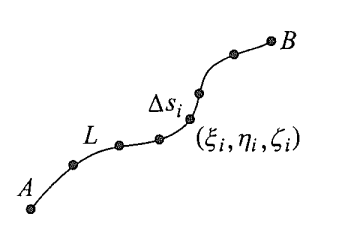
\includegraphics[width=\textwidth]{2.1.png} % 无需重复指定宽度  
\end{myimagebox}     
\caption{\label{fig:2.1}微分的几何意义}   
\end{figure}

从$x\sim x+\Delta x$,函数值从$M\sim M'$。而$f'(x)\Delta x$是函数增加的线性量$\mathrm{d}y$,也就是从$M\sim Q$的变化,而剩下的$M'Q$是函数增量和线性部分的差值,也就是$\Delta x$的高阶无穷小。当$\Delta x\to 0$时,$M',Q$会趋近重合。因此我们利用微分,可以拟合一些函数的值。这也是计算机常用的方法。例如计算$\sqrt{9.1}$的近似值,我们可以找函数$f(x)=\sqrt{x}$,因此$M$代表$\sqrt{9}=3$,而在$x=9$的导数值为$\frac{1}{6}$,因此线性部分为$\frac{0.1}{6}$,因此$\sqrt{9.1}\approx 3+\frac{0.1}{6}$。要注意,这种微分拟合法只在$\Delta x$较小的时候准确。这种微分拟合的思想在泰勒展开中的应用更为广泛。

接下来我们介绍一阶微分形式不变性。我们令$z=g(f(x))$,那么根据复合函数求导法则,我们有:
\begin{align*}
    \mathrm{d}z=g'(f(x))f'(x)\mathrm{d}x
\end{align*}

另一方面,我们把$y=f(x)$看做自变量,则有:
\begin{align*}
    \mathrm{d}z=g'(y)\mathrm{d}y
\end{align*}

这就说明无论$y$是自变量还是中间变量,上面的公式总是成立的,这就是一阶微分形式不变性。这种不变性在多元微分学里面有非常广泛的应用。

一阶微分形式不变性的重要应用在隐函数求导法里面。隐函数是指函数关系并非根据$y=f(x)$给出,而是一个二元函数$f(x;y)=0$给出,那么$y=f(x)$就是这个二元函数的\textbf{隐函数}。例如$x^2+y^2=R^2$ 就有两个隐函数$y=\pm\sqrt{R^2-x^2}$。那么问题来了:怎么在不求隐函数的情况下计算导数?我们看如下例题:

\textbf{例:}设函数$y=f(x)$是由方程$e^{xy}+x^2y-1=0$确定的隐函数,求$y'$。

\textbf{解}:如果我们左右两端求微分,由于$\mathrm{d}xy=y\mathrm{d}x+x\mathrm{d}y$(微分计算法则和导数完全一致),因此左右求微分有:
\begin{align*}
    e^{xy}(y\mathrm{d}x+x\mathrm{d}y)+2xy\mathrm{d}x+x^2\mathrm{d}y=0
\end{align*}

左右两边同时除以$\mathrm{d}x$,则有:
\begin{align*}
    e^{xy}(y+xy')+2xy+x^2y'=0\to y'=-\frac{ye^{xy}+2xy}{xe^{xy}+x^2}
\end{align*}

在函数$y=f(x)$中,我们有时可以把$x,y$看成是新的参数$t$的函数,也就是说:
\begin{tcolorbox}[
    colback=bac1,     % 极浅黄色背景
    colframe=fra1,   % 浅黄色边框
    coltitle=white,             % 标题文字白色
    coltext=tex1,
    title=参数方程,
    fonttitle=\bfseries,        % 标题加粗
arc=3mm,                     % 圆角稍大
breakable
]
参数方程是指由参变量表示自变量$x$和因变量$y$的方程,如:
\begin{align*}
    \begin{cases}
        x=\varphi(t)\\
        y=\psi(t)
    \end{cases}
    \alpha\leq t\leq \beta\tag{2-9}
\end{align*}
\end{tcolorbox}

例如圆$x^2+y^2=R^2$引入参变量$\theta\in[0,2\pi]$,其参变量方程可写作$x=R\cos\theta,y=R\sin\theta$。那么如果我们的参数方程如2-9给出,那么对两个方程求微分(假设都是可微的),则有:
\begin{align*}
    &\mathrm{d}x=\varphi'(t)\mathrm{d}t\qquad \mathrm{d}y=\psi'(t)\mathrm{d}t\\
    &y'=\frac{\mathrm{d}y}{\mathrm{d}x}=\frac{\psi'(t)}{\phi(t)}\tag{2-10}
\end{align*}

\subsubsection{高阶导数和高阶微分}
首先我们简要介绍高阶导数的定义。顾名思义,高阶导数就是“导数的导数",如果函数$y=f(x)$在$x_0$处有一阶导数$f'(x_0)$,如果$x_0$处一阶导数$f'(x_0)$还有导数$f''(x_0)$,称作\textbf{二阶导数}。可以记作$\frac{\mathrm{d}^2 f}{\mathrm{d}x^2}$。例如在物理上,加速度就是直线位移的二阶导数。同理我们可以定义任意的$n$阶导数。

\textbf{例}:计算$\sin x,\cos x,\frac{1}{x},\ln(1+x)$的$n$阶导数。

\textbf{解}:对于$\sin x$,我们求一阶导$\cos x=\sin(x+\frac{\pi}{2})$,再求二阶导$-\sin x=\sin(x+\pi)$,因此利用数学归纳法,假设$(\sin x)^{(n)}=\sin(x+\frac{n\pi }{2})$,那么如果我们证明$n+1$阶导也是这种规律即可(因为起点一阶导满足这个规律)。计算:
\begin{align*}
    \sin'(x+\frac{n\pi}{2})=\cos(x+\frac{n\pi}{2})=\sin(x+\frac{(n+1)\pi}{2})=\sin^{(n+1)}x
\end{align*}

因此数学归纳法证毕。$\cos x$的$n$阶导数就是$\sin x$的$n+1$阶导数,这里不再赘述。同理,$\frac{1}{x}$的$n$阶导数可以写作:
\begin{align*}
    (\frac{1}{x})^{(n)}=(-1)^n\frac{n!}{x^{n+1}}
\end{align*}

利用这种办法,我们也可以计算$f(x)=\frac{2x}{1-x^2}$的高阶导数:
\begin{align*}
    f^{(n)}(x)&=(\frac{1}{1-x})^{(n)}+(\frac{1}{1+x})^{(n)}\\
    &=n!\left[\frac{1}{(1-x)^{n+1}}-\frac{(-1)^n}{(1+x)^{n+1}}\right]
\end{align*}
但一般来说,我们这种办法需要找规律,然后使用数学归纳法。而\textbf{莱布尼茨公式}是计算高阶导数的一个重要办法:
\begin{tcolorbox}[
    colback=bac1,     % 极浅黄色背景
    colframe=fra1,   % 浅黄色边框
    coltitle=white,             % 标题文字白色
    coltext=tex1,
    title=Leibniz公式,
    fonttitle=\bfseries,        % 标题加粗
arc=3mm,                     % 圆角稍大
breakable
]
设函数$f(x),g(x)$在区间$(a,b)$有$n$阶导数,则它们之积的$n$阶导数满足下面的公式(定义0阶导数是函数本身):
\begin{align*}
    [f(x)g(x)]^{(n)}=\sum_{k=0}^n C_n^kf^{(k)}(x)g^{(n-k)}(x)\tag{2-11}
\end{align*}

这与二项式定理的形式类似。
\end{tcolorbox}

这个定理的证明采用数学归纳法。当$n=1$时,$(fg)'=f'g+fg'$,符合等式右侧的形式。假设$n=m$成立,我们现在需要说明$n=m+1$也成立。代入$n=m$右侧的形式再求一次导数:
\begin{align*}
    [f(x)g(x)]^{(m+1)}&=\left[\sum_{k=0}^m C_m^kf^{(k)}(x)g^{(m-k)}(x)\right]'\\
&=\left[\sum_{k=0}^m C_m^kf^{(k+1)}(x)g^{(m-k)}(x)\right]+\left[\sum_{k=0}^m C_m^kf^{(k)}(x)g^{(m-k+1)}(x)\right]\\
&=C_m^0 f(x)g^{(m+1)}(x)+C_m^m f^{(m+1)}(x)g(x)+\left[\sum_{k=1}^{m-1}(C_m^k+C_{m}^{k-1})f^{(k)}(x)g^{(m-k+1)}(x)\right]\\
&=\sum_{k=0}^{m+1} C_{m+1}^kf^{(k)}(x)g^{(m-k+1)}(x)
\end{align*}

最后一个等号使用了组合数公式$C_m^k+C_{m}^{k-1}=C_{m+1}^k$。

\textbf{例:}计算(1)$(x^2\sin x)^{(80)}$。(2)若$y=\arcsin x$,求$y^{(n)}(0)$。

\textbf{解:}显然$x^2$在三阶导的时候就已经变为0了,因此:
\begin{align*}
    f^{(80)}(x)&=C_{80}^0x^2\sin x^{(80)}+C_{80}^1 2x\sin x^{79}+C_{80}^22\sin x^{(78)}\\
    &=(x^2-6320)\sin x-160x\cos x
\end{align*}

第二题会更复杂,因为直接计算很难找出规律,我们先求一阶导$y'=\frac{1}{\sqrt{1-x^2}}$,改写为$y'\sqrt{1-x^2}=1$,然后等式左右求导后,整理得到:
\begin{align*}
    (1-x^2)y''-xy'=0
\end{align*}

我们得到了\textbf{一阶导数和二阶导数的关系,然后对等式左侧使用莱布尼茨法则}:
\begin{gather*}
    y^{(n+2)}(1-x^2)+ny^{(n+1)}(-2x)+\frac{n(n-1)}{2}y^{(n)}(-2)-(xy^{n+1}+ny^{(n)})=0\\
(1-x^2)y^{(n+2)}-(2n+1)xy^{(n+1)}-n^2y^{(n)}=0 
\end{gather*}

代入$x=0$就可以得到\textbf{递推公式}:
\begin{align*}
    y^{(n+2)}(0)-n^2y^{(n)}(0)=0
\end{align*}

然后观察初值条件,由于$y(0)=0,y'(0)=1$。因此得到:
\begin{align*}
    y^{(2k)}(0)=0\qquad y^{(2k+1)}(0)=[(2k-1)!!]^2
\end{align*}

其中$!!$是\textbf{双阶乘符号},代表着从这个数开始隔一个数字乘一下直到2或者1,例如$5!!=5\cdot 3\cdot1,4!!=4\cdot 2$。

高阶微分的计算方法与高阶导数类似,由于:
\begin{align*}
    \frac{\mathrm{d}^n f}{\mathrm{d}x^n}=f^{(n)}(x)
\end{align*}

我们把$\mathrm{d}x^n$乘到等式右边,就得到了高阶微分的表达式。然而高阶微分没有形式不变性。

\textbf{例:}函数$y=e^x\cos 2x$,计算$\mathrm{d}^2y$

\textbf{解:}我们计算二阶导数$y''=-3e^x\cos 2x-4e^x\sin 2x$,因此$\mathrm{d}^2y=\mathrm{d}x^2 y''$。

\subsection{习题补充与拓展}
本章的重点是理解\textbf{导数的定义}(有些分段函数的导数不能用导数公式),\textbf{可导性和连续性,用特殊方法求导数和高阶导数}。

\textbf{例1}:设$n$为正整数,判断在什么条件下下面的函数在$x=0$连续;可导;导函数连续。
\begin{align*}
    f(x)=\begin{cases}
        x^n\sin\frac{1}{x} & x\neq 0\\
        0 &x=0
    \end{cases}
\end{align*}

\textbf{解}:本题是对可导和连续关系的经典题目。对于连续性,由于$x\to 0$时,$|\sin \frac{1}{x}|\leq 1$,因此$|f(x)|\leq x^n$,因此若$|f(x)|<\varepsilon$,只需满足$\delta^n<\varepsilon$,即$x\in(-\delta,\delta)$上满足误差要求。因此连续性是可以一直保证的。

由于这是一个分段函数,因此不能对其单纯求导。当$n=1$时,如果在0处可导,我们需要计算下面的极限:
\begin{align*}
     \lim_{\Delta x\to 0}\frac{f(0+\Delta x)-f(0)}{\Delta x}=  \lim_{\Delta x\to 0}\sin \frac{1}{\Delta x}
\end{align*}

显然这个极限是不存在的,因此不可导。而$n\geq 2$时,同理可以证明是可导的。对于第三问首先$n\geq 2$是必要的,此时在$x\neq 0$处有:
\begin{align*}
    f'(x)=nx^{n-1}\sin\frac{1}{x}-x^{n-2}\cos\frac{1}{x}
\end{align*}

当$n=2$时,由于$x\to 0$时$2x\sin \frac{1}{x}-\cos\frac{1}{x}$并不趋近于0,导数不连续。而当$n\geq 3$时,导数连续。

\textbf{例2}:若$n$是正整数,证明对于下面的函数$f(x)$满足$f^{(n)}(0)=0$
\begin{align*}
    f(x)=\begin{cases}
        e^{-\frac{1}{x^2}}& x\neq 0\\
        0 & x=0
    \end{cases}
\end{align*}

\textbf{解}:这道题也非常经典。首先我们计算$f'(x)$,由于分段函数,因此在$x=0$处要分开讨论。在$x=0$处利用导数的定义:
\begin{align*}
f'(0)=\lim_{x\to 0}\frac{1}{x}\cdot e^{-\frac{1}{x^2}}=\lim_{y\to \infty}e^{-y^2}=0  
\end{align*}

而当$x\neq 0$时,直接求导:
\begin{align*}
    f'(x)=\frac{2}{x^3}e^{-\frac{1}{x^2}}
\end{align*}

接下来我们计算二阶导数。在0处也需要利用导数的定义:
\begin{align*}
    f''(0)=\lim_{x\to 0}\frac{f'(x)-f'(0)}{x}=\lim_{x\to 0}\frac{2}{x^4}e^{-\frac{1}{x^2}}=0
\end{align*}

而在非0处直接求导:
\begin{align*}
    f''(x)=(\frac{4}{x^6}-\frac{6}{x^4})e^{-\frac{1}{x^2}}
\end{align*}

因此我们可以推断函数$n$阶导数在$x\neq 0$的形式为:
\begin{align*}
    f^{(n)}(x)=P_n(\frac{1}{x})e^{-\frac{1}{x^2}}
\end{align*}

其中符号$P_n(y)$是指关于$y$的多项式。这个结论的证明利用数学归纳法。我们在这道题结束的时候补充。我们接下来算$f^{(n)}(0)$。当$n=1,2$的时候显然成立,假设$n=k$时也成立,对于$n=k+1$,利用导数的定义:

\begin{align*}
f^{(k+1)}(0)=\lim_{x\to 0}\frac{f^{(k)}(x)-f^{(k)}(0)}{x}=\lim_{x\to 0}\frac{1}{x}P_k(\frac{1}{x})e^{-\frac{1}{x^2}}\to 0 
\end{align*}

因此数学归纳法,原命题证毕。
\begin{tcolorbox}[
    colback=bac2,     % 极浅黄色背景
    colframe=fra2,   % 浅黄色边框
    coltitle=white,             % 标题文字白色
    coltext=tex2,
    title=补充证明:数学归纳法证明高阶导数的形式,
    fonttitle=\bfseries,        % 标题加粗
arc=3mm,                     % 圆角稍大
breakable
]
当$n=1,2$结论显然。假设$n=k$时结论成立,那么计算$k+1$阶导数:
\begin{align*}
f^{(k+1)}(x)&=\left[P_k(\frac{1}{x})e^{-1/x^2} \right]'=P_k'(\frac{1}{x})(-\frac{1}{x^2})e^{-1/x^2}
+P_k(\frac{1}{x})\cdot \frac{2}{x^3}\cdot e^{-1/x^2}\\
&=[P_k(y)(-y)^2+P_k(y)(2y^3)]|_{y=\frac{1}{x} }\cdot e^{-1/x^2}\\
&=P_{k+1}(\frac{1}{x}) \cdot e^{-1/x^2}
\end{align*}
\end{tcolorbox}

\textbf{例3}:设函数$y=y(x)$可导,且满足方程$x^2+xy+y^2=1$,求$y''$。并设置合理的参数方程去计算$y_x''$,比较二者答案是否一致。

\textbf{解}:直接使用隐函数求导法,两边都对$x$求导,得到:
\begin{align*}
    2x+y+xy'+2yy'=0\to y'=-\frac{2x+y}{x+2y}
\end{align*}

然后继续对上面式子求导并带入$y'$的表达式。可以得到:
\begin{align*}
    y''=-\frac{6}{(x+2y)^3}
\end{align*}

另一方面我们也可以用参数方程法,原方程可写作$(y+\frac{1}{2}x)^2+\frac{3}{4}x^2=1$,因此令$y+\frac{1}{2}x=\sin t,\frac{\sqrt{3}}{2}x=\cos t$,解得参数方程的形式为:
\begin{align*}
    x=\frac{2}{\sqrt{3}}\cos t\qquad y=\sin t-\frac{1}{\sqrt{3}}\sin t
\end{align*}

因此计算一阶导的表达式如下:
\begin{align*}
    y'=\frac{\mathrm{dy}/\mathrm{d}t}{\mathrm{d}x/\mathrm{d}t}=-\frac{\sqrt{3}}{2}\cot t-\frac{1}{2}
\end{align*}

按照同样的方式计算二阶导数:
\begin{align*}
    y''=-\frac{3}{4}\csc^3 t\qquad (\csc t=\sin^{-1}t)
\end{align*}

\textbf{例4}:计算下面函数的$n$阶导数:
\begin{align*}
    (1) y=\sin ^3 x \qquad (2) y=\frac{x^n}{1-x}
\end{align*}

\textbf{解}:第一题利用三倍角公式:
\begin{tcolorbox}[
    colback=bac1,     % 极浅黄色背景
    colframe=fra1,   % 浅黄色边框
    coltitle=white,             % 标题文字白色
    coltext=tex1,
    title=三倍角公式,
    fonttitle=\bfseries,        % 标题加粗
arc=3mm,                     % 圆角稍大
breakable
]
三倍角公式的内容如下:
\begin{align*}
    \sin 3\theta=3\sin\theta-4\sin^3\theta\\
    \cos 3\theta=4\cos^3\theta-3\cos\theta\tag{2-12}
\end{align*}
\end{tcolorbox}

因此就有:
\begin{align*}
    y^{(n)}(x)&=\frac{3}{4}\sin^{(n)}x-\frac{1}{4}\sin^{(n)}3x=\frac{3}{4}\sin(x+\frac{n\pi}{2})-\frac{3^n}{4}\sin(3x+\frac{n\pi}{2})
\end{align*}

第二题直接使用莱布尼茨公式即可,当然还有一种巧妙的办法:
\begin{align*}
    y=-\sum_{k=0}^{n-1}x^k+\frac{1}{1-x}\to y^{(n)}(x)=\frac{(-1)^{n+1}n!}{(1-x)^{n+1}}
\end{align*}

\textbf{例5}:(1)已知$y=\arctan x$,计算$y^{(n)}(0)$

(2)已知$y=\arctan^2 x$,计算$y^{(n)}(0)$

\textbf{解}:对$\arctan x$求导,得到$(1+x^2)y'=1$,然后对两边求$n-1$阶导数,根据莱布尼茨公式有:
\begin{align*} 
  (1+x^2)y^{(n)}+(n-1)\cdot 2x\cdot y^{(n-1)}+(n-1)(n-2)\cdot y^{(n-2)}=0
\end{align*}

代入$x=0$得到:
\begin{align*}
    y^{(n)}(0)=-(n-1)(n-2)y^{(n-2)}(0)
\end{align*}

结合初值条件$y(0)=0,y'(0)=1$可以得到:
\begin{align*}
    y^{(n)}(0)=\begin{cases}
        0 & n=2k\\
        (-1)^k(2k)! &n=2k+1
    \end{cases}
\end{align*}

第二题直接对$(\arctan x\cdot \arctan x)$做莱布尼茨公式,则有:
\begin{align*}
    y^{(n)}(0)=0
\end{align*}

\textbf{例6:}设函数$f(x)$在点$a$可导并且$f(a)\neq 0$,证明下面结论:
\begin{align*}
    \lim_{n\to\infty}\left[\frac{f(a+\frac{1}{n})}{f(a)}\right]^n=\exp\frac{f'(a)}{f(a)}
\end{align*}

(2)设函数$f$在实数域上有任意阶导数,证明对每个正整数$n$都有:
\begin{align*}
    \frac{1}{x^{n+1}}f^{(n)}(\frac{1}{x})=(-1)^n[x^{n-1}f(\frac{1}{x})]^{(n)}
\end{align*}

\textbf{解:}(1)我们证明等号两侧取对数的极限是一样的,即:
\begin{align*} 
 \lim_{n\to\infty}\frac{\ln\frac{f(a+1/n)}{f(a)} }{1/n}&=\lim_{n\to\infty}\frac{\ln\left[1+\frac{f(a+1/n)-f(a)}
{f(a)}\right] }{1/n}\\
&= \lim_{n\to\infty}\frac{\frac{f(a+1/n)-f(a)}
{f(a)} }{1/n}\\
&=\lim_{n\to\infty}\frac{\frac{f(a+1/n)-f(a)}
{1/n} }{f(a)}\\
&=\frac{f'(a)}{f(a)} 
\end{align*}

第二个等号能成立是因为使用了等价无穷小$\ln(1+x)\sim x$。

(2)这道题需要使用数学归纳法。当$n=0$时,结论显然成立。我们假设结论对$n-1$也成立,即就是:
\begin{align*}
    \frac{1}{x^{n}}f^{(n-1)}(\frac{1}{x})=(-1)^{n-1}[x^{n-2}f(\frac{1}{x})]^{(n-1)}
\end{align*}

然后对两边同时求导,得到:
\begin{gather*}
       -\frac{1}{x^{n+2}}f^{(n)}(\frac{1}{x})-\frac{n}{x^{n+1}}f^{(n-1)}(\frac{1}{x})=(-1)^{n-1}
[x^{n-2}f(\frac{1}{x})]^{(n)}    \\
 \frac{1}{x^{n+1}}f^{(n)}(\frac{1}{x})=(-1)^{n}x[x^{n-2}f(\frac{1}{x})]^{(n)}-\frac{n}{x^{n}}f^{(n-1)}(\frac{1}{x}) 
\end{gather*}

又因为:
\begin{align*}
 \left[ x^{n-1}f(\frac{1}{x})\right]^{(n)}&=  \left[ x\cdot x^{n-2}f(\frac{1}{x})\right]^{(n)}\\
&=x \left[ x^{n-2}f(\frac{1}{x})\right]^{(n)}+ n\left[ x^{n-2}f(\frac{1}{x})\right]^{(n-1)}\\
&=x \left[ x^{n-2}f(\frac{1}{x})\right]^{(n)}+n\cdot (-1)^{n-1}\cdot\frac{1}{x^{n}}f^{(n-1)}(\frac{1}{x})
\end{align*}

证毕。

\textbf{例7}:证明在曳物线$x=a(\ln\tan\frac{t}{2}+\cos t),y=a\sin t$的每一条切线从切点到与$x$轴的交点的长度为一常数。
\begin{figure}[H]    
\centering     
\renewcommand{\figurename}{图}     
\renewcommand{\thefigure}{2.2}    
\begin{myimagebox}[width=0.35\textwidth] % 直接传入图片尺寸参数      
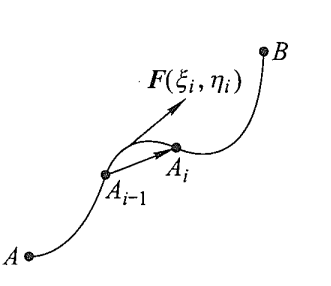
\includegraphics[width=\textwidth]{2.2.png} % 无需重复指定宽度  
\end{myimagebox}     
\caption{\label{fig:2.2}曳物线}   
\end{figure}

\textbf{解:}直接计算$y_x$($y$对$x$的导数):
\begin{align*}
 \frac{\mathrm{d}y }{\mathrm{d}x }&=\frac{\mathrm{d}y/\mathrm{d}t  }{\mathrm{d}x/\mathrm{d}t }
=\frac{a\cos t}{a\left(\frac{1}{\tan (t/2)}\cdot\frac{1}{\cos^2(t/2)}-\sin t  \right)} \\
&=\frac{\cos t}{\frac{1+\cos t}{\sin t}\cdot\frac{1}{1+\cos t}-\sin t }\\
&=\tan t  
\end{align*}

因此确定参数$t$,曲线的切线为:
\begin{align*}
y-a\sin t=\tan t\left[x-a\ln(\tan\frac{t}{2}+\cos t) \right]
\end{align*}

令$y=0$,则$x=a\ln(\tan\frac{t}{2}+\cos t)-a\cos t$,则距离$l$为:
\begin{align*}
l&=\sqrt{1+\tan^2 t} \cdot\left|a\ln(\tan\frac{t}{2}+\cos t) -a\cos t-a\ln(\tan\frac{t}{2}+\cos t)\right|\\
&=a
\end{align*}

\textbf{例8}:(1)设$n\geq 2$,函数$f(x)=f(x_0)+\varphi(x)(x-x_0)$在某邻域$O(x_0)$上$n-1$阶可微,且$\varphi^{(n-1)}(x)$在$x_0$处连续。证明$f(x)$在$x_0$上$n$阶可导。

(2)设多项式函数$p(x)$只有实零点,证明$\forall x\in\mathbb{R}$都有:
\begin{align*}
    [p'(x)]^2-p(x)p''(x)\geq 0
\end{align*}

\textbf{解}:(1)我们在邻域内同时求$n-1$阶导数,就有:
\begin{align*}
f^{(n-1)}(x)=\varphi^{(n-1)}(x)(x-x_0)+(n-1)\varphi^{(n-2)}(x)
\end{align*}

而$\varphi^{(n-2)}(x)$是可导的,因此我们只需说明$\varphi^{(n-1)}(x)(x-x_0)+(n-1)$也可导即可。由于$\varphi^{(n-1)}(x)$在$x=x_0$处连续,因此利用导数定义:
\begin{align*}
\lim_{x\to x_0}\frac{\varphi^{(n-1)}(x)}{x-x_0}=\lim_{x\to x_0} \varphi^{(n-1)}(x)=\varphi^{(n-1)}(x_0)
\end{align*}

因此也是可导的,原命题证毕。

(2)设多项式为$p(x)=(x-x_1)(x-x_2)...(x-x_n)$(最高次系数不为1不影响结果),根据复合函数求导法则,有:
\begin{align*}
    p'(x)=p(x)\sum_{k=1}^n\frac{1}{x-x_k}
\end{align*}

对两边继续求导,得到二阶导形式:
\begin{align*}
p''(x)=p'(x)\sum_{k=1}^n\frac{1}{x-x_k}-p(x)\sum_{k=1}^\infty\frac{1}{(x-x_k)^2}  
\end{align*}

因此当$p(x)\neq 0$时,计算$p(x)p''(x)$有:
\begin{align*}
p(x)p''(x)&=p(x)p'(x)\sum_{k=1}^n\frac{1}{x-x_k}-[p(x)]^2\sum_{k=1}^\infty\frac{1}{(x-x_k)^2} \\
 &=[p'(x)]^2-[p(x)]^2\sum_{k=1}^\infty\frac{1}{(x-x_k)^2}\\
&=[p'(x)]^2\left[1-\frac{\sum_{k=1}^n\frac{1}{(x-x_k)^2}}{(\sum_{k=1}^n\frac{1}{x-x_k})^2} \right]\\
&\leq [p'(x)]^2
\end{align*}

故原不等式成立。

\section{微分中值定理与泰勒展开}
\subsection{微分中值定理}
\subsubsection{微分中值定理的内容和证明}
微分中值定理是微分学的基石,我们在这里介绍Rolle定理,Largrange中值定理,Cauchy中值定理。本部分将对这三个定理的\textbf{内容、证明、应用}进行讲解,读者应该对这三部分都要有较好的掌握。

在学习微分中值定理前,我们先介绍Fermat定理:
\begin{tcolorbox}[
    colback=bac1,     % 极浅黄色背景
    colframe=fra1,   % 浅黄色边框
    coltitle=white,             % 标题文字白色
    coltext=tex1,
    title=Fermat定理,
    fonttitle=\bfseries,        % 标题加粗
arc=3mm,                     % 圆角稍大
breakable
]
设$x_0$是$f(x)$的极值点,且存在导数$f'(x_0)$,则$f'(x_0)=0$。
\end{tcolorbox}

我们接下来证明:不妨假设$x_0$是极小值点,则$\exists \delta>0,|x-x_0|<\delta$时有$f(x)\geq f(x_0)$。由于导数$f'(x_0)$存在,则左导数和右导数存在且相等。另一方面:
\begin{align*}
    \lim_{x\to x_0}\frac{f(x)-f(x_0)}{x-x_0}=f'(x_0)
\end{align*}

那么右导数在$x\to c+0$时小于等于0,左导数大于等于0。而这一点可导要求左极限与右极限相等,因此$f'(x_0)=0$。

Fermat定理是证明Rolle定理的工具:
\begin{tcolorbox}[
    colback=bac1,     % 极浅黄色背景
    colframe=fra1,   % 浅黄色边框
    coltitle=white,             % 标题文字白色
    coltext=tex1,
    title=Rolle罗尔定理,
    fonttitle=\bfseries,        % 标题加粗
arc=3mm,                     % 圆角稍大
breakable
]
设函数$f(x)$在闭区间$[a,b]$连续,在$(a,b)$上可微,且有$f(a)=f(b)$,则$\exists \xi \in (a,b)$,使得$f'(\xi)=0$。
\end{tcolorbox}
\begin{figure}[H]    
\centering     
\renewcommand{\figurename}{图}     
\renewcommand{\thefigure}{3.1}    
\begin{myimagebox}[width=0.44\textwidth] % 直接传入图片尺寸参数      
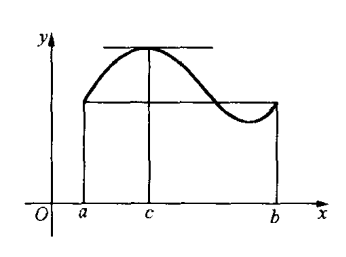
\includegraphics[width=\textwidth]{3.1.png} % 无需重复指定宽度  
\end{myimagebox}     
\caption{\label{fig:3.1}罗尔定理的几何意义}   
\end{figure}

图3.1从函数图象的角度展示了罗尔定理。我们接下来对罗尔定理进行证明:如果函数$f(x)$是常值函数,那么$\forall x\in(a,b),f'(x)=0$已经满足题设要求。否则在有界闭区间上,函数$f(x)$一定可以取到最大值$M$和最小值$m$。假设最大值在$(a,b)$里面达到,这就是说$\exists c\in (a,b),\forall x\in[a,b],f(x)\leq f(c)$。由于函数在$c$处可导,则:
\begin{align*}
    \lim_{x\to c}\frac{f(x)-f(c)}{x-c}=f'(c)
\end{align*}

由于$f(x)\leq f(c)$,那么右导数在$x\to c+0$时小于等于0,左导数大于等于0。而这一点可导要求左极限与右极限相等,因此$f'(c)=0$。当$f(x)$最小值在$(a,b)$内达到时同理。

Largrange中值定理的内容包含了Rolle定理,其表述内容如下:
\begin{tcolorbox}[
    colback=bac1,     % 极浅黄色背景
    colframe=fra1,   % 浅黄色边框
    coltitle=white,             % 标题文字白色
    coltext=tex1,
    title=Largrange拉格朗日中值定理,
    fonttitle=\bfseries,        % 标题加粗
arc=3mm,                     % 圆角稍大
breakable
]
设函数$f$在区间$[a,b]$上连续,在$(a,b)$可微,则$\exists \xi\in(a,b)$使得:
\begin{align*}
    f'(\xi)=\frac{f(b)-f(a)}{b-a}\tag{3-1}
\end{align*}
\end{tcolorbox}
\begin{figure}[H]    
\centering     
\renewcommand{\figurename}{图}     
\renewcommand{\thefigure}{3.2}    
\begin{myimagebox}[width=0.44\textwidth] % 直接传入图片尺寸参数      
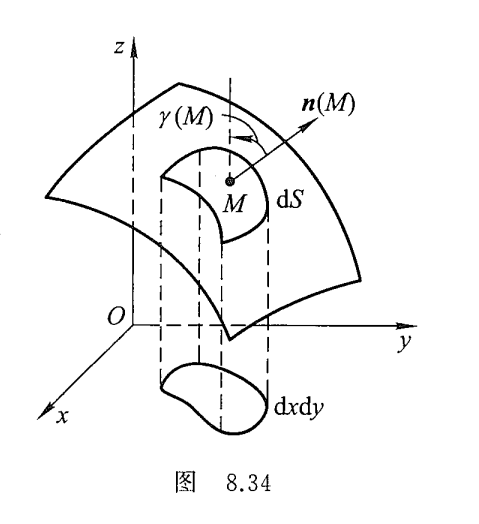
\includegraphics[width=\textwidth]{3.2.png} % 无需重复指定宽度  
\end{myimagebox}     
\caption{\label{fig:3.2}拉格朗日中值定理的几何意义}   
\end{figure}

图3.2展示了拉格朗日中值定理的几何意义。拉格朗日中值定理的证明是非常重要的,因为它考察了对\textbf{辅助函数的构造}(这也是微分中值定理应用时非常重要的一环)。令:
\begin{align*}
    g(x)=(b-a)f(x)-[f(b)-f(a)](x-a)
\end{align*}

则有$g(a)=g(b)=a(b-a)$,另一方面函数$g(x)$在$(a,b)$上可微,因此根据\textbf{罗尔定理},$\exists \xi \in(a,b)$使得:
\begin{align*}
    g'(\xi)&=(b-a)f'(\xi)-f(b)+f(a)=0\\
    f'(\xi)&=\frac{f(b)-f(a)}{b-a}
\end{align*}

利用拉格朗日中值定理,我们能得到如下推论:
\begin{tcolorbox}[
    colback=bac2,     % 极浅黄色背景
    colframe=fra2,   % 浅黄色边框
    coltitle=white,             % 标题文字白色
    coltext=tex2,
    title=推论,
    fonttitle=\bfseries,        % 标题加粗
arc=3mm,                     % 圆角稍大
breakable
]
设函数$f(x)$在$(a,b)$可导并且导函数$f'(x)\equiv 0$,则$f(x)\equiv c$
\end{tcolorbox}

利用拉格朗日中值定理可以证明,$\forall x\in(a,b)$,$\exists c\in(a,x)$,使得:
\begin{align*}
    f(x)=f(a)+f'(c)(x-a)=f(a)
\end{align*}

同时我们也能得到,若函数在$[a,b]$连续并且在$(a,b)$可导,如果$f'(x)>0$(也可以在有限个点上等于0),那么函数严格递增。反之亦然。

利用Largrange中值定理和Fermat定理,我们可以证明\textbf{Darboux定理}:
\begin{tcolorbox}[
    colback=bac2,     % 极浅黄色背景
    colframe=fra2,   % 浅黄色边框
    coltitle=white,             % 标题文字白色
    coltext=tex2,
    title=Darboux达布定理,
    fonttitle=\bfseries,        % 标题加粗
arc=3mm,                     % 圆角稍大
breakable
]
设函数$f(x)$在闭区间$[a,b]$可导,且$f'(a)=A,f'(b)=B$。则对于在$A$和$B$中的任意一个值$C$,都$\exists c\in[a,b]$,使得$f'(c)=C$。并且这\textbf{不要求导数是连续的}!
\end{tcolorbox}

其证明过程如下:不妨假设$A<C<B$,构造辅助函数:
\begin{align*}
    g(x)=f(x)-C(x)
\end{align*}

那么$g'(x)=f'(x)-c$,我们只需证明$g'(x)$在$[a,b]$上有零点。代入端点值得到$g'(a)<0,g'(b)>0$。因为$g(x)$在闭区间上可导,因此$g(x)$一定连续。根据端点导数的定义,则$g'(x)$在端点邻域$(a,a+\delta)$内导数小于0,也就是说$g(x)$在$(a,a+\delta)$范围内递减。另一方面在$(b-\delta,b)$上函数递增。因此最小值一定在开区间$(a,b)$内。因此根据Fermat定理证毕。

接下来我们讲述Cauchy中值定理:
\begin{tcolorbox}[
    colback=bac1,     % 极浅黄色背景
    colframe=fra1,   % 浅黄色边框
    coltitle=white,             % 标题文字白色
    coltext=tex1,
    title=Cauchy柯西中值定理,
    fonttitle=\bfseries,        % 标题加粗
arc=3mm,                     % 圆角稍大
breakable
]

设函数$f(x),g(x)$在$[a,b]$上连续,且在$(a,b)$上可微,且满足条件$g(b)\neq g(a)$,$f'^2(x)+g'^2(x)\neq 0,\forall x\in(a,b)$,则$\exists \xi\in(a,b)$使得:
\begin{align*}
    \frac{f(b)-f(a)}{g(b)-g(a)}=\frac{f'(\xi)}{g'(\xi)}\tag{3-3}
\end{align*}
\end{tcolorbox}

不妨记3-3左侧式子为$\lambda$,我们实则是需要证明$f'(\xi)-\lambda g'(\xi)=0$,因此构造辅助函数:
\begin{align*}
    F(x)=f(x)-\lambda g(x)
\end{align*}

然后计算端点值:
\begin{align*}
    F(a)=\frac{f(a)g(b)-f(b)g(a)}{g(b)-g(a)}\qquad  F(b)=\frac{f(a)g(b)-f(b)g(a)}{g(b)-g(a)}
\end{align*}

利用Rolle定理证毕。

\subsubsection{微分中值定理的应用}
这部分我们会利用几道例题来介绍微分中值定理的应用:

\textbf{例}:设$\frac{a_0}{n+1}+\frac{a_1}{n}+...+a_n=0$,证明下面的方程在区间$(0,1)$至少有一个实根:
\begin{align*}
    f(x)=a_0x^n+a_1x^{n-1}+..+a_n=0
\end{align*}

\textbf{解}:我们构造辅助函数:
\begin{align*}
    F(x)=\frac{a_0x^{n+1}}{n+1}+\frac{a_1x^n}{n}+...+a_nx
\end{align*}

可以得到$F(0)=F(1)=0$,$F(x)$在$[0,1]$连续$(0,1)$可微。因此根据Rolle定理,$\exists \xi\in(0,1)$使得$F'(\xi)=0$,原命题证毕。因此辅助函数构造的本质是\textbf{原函数的积分函数}。

\textbf{例}:设函数$f$在闭区间$[a,b]$上二阶可微,且$f(a)=f(b)=0$,证明$\forall x\in(a,b),\exists \xi\in(a,b)$使得:
\begin{align*}
    f(x)=\frac{f''(\xi)}{2}(x-a)(x-b)
\end{align*}

\textbf{解}:\textbf{固定}$x$,令$\lambda=\frac{2f(x)}{(x-a)(x-b)}$,于是只用证明$\xi\in(a,b)$使得$f''(\xi)=\lambda$成立。因此构造辅助函数:
\begin{align*}
    F(t)=f(t)-\frac{\lambda}{2}(t-a)(t-b)\qquad t\in[a,b]
\end{align*}

由条件$f(a)=f(b)=0$,因此$F(a)=F(b)=0$。根据$\lambda$定义可以得到$F(x)=0$。因此在$[a,x],[x,b]$上分别用Rolle定理,即$\exists \eta_1,\eta_2$使得$F'(\eta_1)=F'(\eta_2)=0,a<\eta_1<x<\eta_2<b$。而在$[\eta_1,\eta_2]$对导数$F'$用罗尔定理,则$\exists \xi\in[\eta_1,\eta_2]$使得$F''(\xi)=0$,证毕。

\textbf{例:}设函数$f\in C[0,1]$且在$(0,1)$可微,并且$f(0)=0,f(1)=1$。又设$k_1,k_2...k_n$是满足$\sum_{i=1}^n k_i=1$的$n$个整数。证明在$(0,1)$中有$n$个互不相同的数$t_1,t_2...t_n$使得:
\begin{align*}
    \frac{k_1}{f'(t_1)}+\frac{k_2}{f'(t_2)}+...+\frac{k_n}{f'(t_n)}=1
\end{align*}

\textbf{解:}根据连续函数截止定理,我们可以找到$0=x_0<x_1<x_2<...<x_{n-1}<x_n=1$,使得$f(x_i)=\sum_{m=1}^i k_m$。而在区间$[x_i,x_{i+1}]$上使用Lagrange中值定理,有$t_1,t_2...t_n$:
\begin{align*}
    k_i=f(x_i)-f(x_i-1)=f'(t_i)(x_i-x_{i-1})
\end{align*}

这样就有:
\begin{align*}
     \frac{k_1}{f'(t_1)}+\frac{k_2}{f'(t_2)}+...+\frac{k_n}{f'(t_n)}=(x_1-x_0)+(x_2-x_1)+...+(x_n-x_{n-1})=1
\end{align*}

\textbf{例:}(1)设函数$f(x)$在$[a,+\infty)$上连续,在$(a,+\infty)$上可微。且$\lim_{x\to+\infty}f(x)=f(a)$。证明$\exists \xi >a$,使得$f'(\xi)=0$。

(2)证明Laguerre多项式$L_n(x)=e^x(x^n e^{-x})^{(n)}$有$n$个正根。

\textbf{解}:(1)我们的突破口在连续和极限的定义上。这个题的重点就是解析这两个条件的含义。

假设$\exists \eta\in(a,+\infty)$,使得$f(\eta)=f(a)$,那么在$[a,\eta]$上直接使用Rolle定理即可证明。如果不存在,那么说明函数恒大于或者恒小于$f(a)$。

不妨令函数恒大于$f(a)$。那么在$a$处的连续性可以解释成:$\forall \varepsilon>0,\exists \delta,\forall |x-a|<\delta,|f(x)-f(a)|<\varepsilon$。因此我们能在$[a,a+\delta)$上找到一点$x_1$使得$f(x_1)=f(a)+\frac{1}{2}\varepsilon$。趋近于无穷的极限其数学语言为:$\forall \varepsilon>0,\exists x_0,\forall x>x_0,|f(x)-f(a)|<\varepsilon$。因此$\exists x_2>x_0$使得$f(x_2)=f(a)+\frac{1}{2}\varepsilon$。因此$f(x_1)=f(x_2)$,在这个区间使用Rolle定理即可。

\begin{tcolorbox}[
    colback=bac1,     % 极浅黄色背景
    colframe=fra1,   % 浅黄色边框
    coltitle=white,             % 标题文字白色
    coltext=tex1,
    title=一点补充,
    fonttitle=\bfseries,        % 标题加粗
arc=3mm,                     % 圆角稍大
breakable
]
第一问的内容本质上是Rolle定理在无限区间上的推广,其内容和条件与Rolle定理类似。
\end{tcolorbox}

(2)利用第一问对Rolle定理的推广,记函数$f(x)=x^ne^{-x}$,则不难验证对于任意的$k,1\leq k\leq n$都有$f^{(n)}(0)=\lim_{x\to\infty}f^{(n)}=0$。因此利用Rolle定理的推论即可证明。

\begin{tcolorbox}[
    colback=bac2,     % 极浅黄色背景
    colframe=fra2,   % 浅黄色边框
    coltitle=white,             % 标题文字白色
    coltext=tex2,
    title=小拓展——关于Laguerre多项式,
    fonttitle=\bfseries,        % 标题加粗
arc=3mm,                     % 圆角稍大
breakable
]
Laguerre多项式满足这样的递推关系:
\begin{align*}
    L_{n+1}(x)=(2n+1-x)L_n(x)-n^2L_{n-1}(x)
\end{align*}

其精确的表达式为:
\begin{align*}
    L_n(x)=\sum_{k=0}^\infty (-1)^kC_n^k\cdot\frac{n!}{k!}\cdot x^k
\end{align*}
\end{tcolorbox}

\textbf{例}:设函数$f(x)$在$[a,b]$连续且在$(a,b)$可微,且有$0<a<b$。证明$\exists \xi\in(a,b)$使得下式成立:
\begin{align*}
    f(b)-f(a)=\ln\frac{b}{a}\cdot \xi f'(\xi)
\end{align*}

\textbf{解}:Cauchy中值定理的隐蔽性在于需要自行寻找$g(x)$,由于$\ln b-\ln a=\ln\frac{b}{a}$。因此令$g(x)=\ln x$,则有:
\begin{align*}
    \frac{f(b)-f(a)}{\ln b-\ln a}=\frac{f'(\xi)}{g'(\xi)}
\end{align*}

\subsection{洛必达法则和泰勒展开}
\subsubsection{洛必达法则}
洛必达法则在高中时已经有所应用,这里我们直接给出洛必达法则的内容,并且利用Cauchy中值定理进行证明:
\begin{tcolorbox}[
    colback=bac1,     % 极浅黄色背景
    colframe=fra1,   % 浅黄色边框
    coltitle=white,             % 标题文字白色
    coltext=tex1,
    title=L'Hospital洛必达法则,
    fonttitle=\bfseries,        % 标题加粗
arc=3mm,                     % 圆角稍大
breakable
]
设函数$f(x),g(x)$在点$a$的一个空心邻域内有定义并且可导,并且$g'(x)\neq 0$。假若$\lim_{x\to a}f(x)=\lim_{x\to \infty}g(x)=0/\infty$(也就是说$\frac{f(x)}{g(x)}$是$\frac{0}{0}/\frac{\infty}{\infty}$)未定式,并且$x\to a$时,\textbf{$\frac{f'(x)}{g'(x)}$极限存在},则当$x\to a$时$\frac{f(x)}{g(x)}$极限存在,并且有:
\begin{align*}
    \lim_{x\to a}\frac{f(x)}{g(x)}=\lim_{x\to a}\frac{f'(x)}{g'(x)}\tag{3-4}
\end{align*}
\end{tcolorbox}

注意在洛必达法则中,我们强调\textbf{$\frac{f'(x)}{g'(x)}$极限存在},例如下面的例子:

\textbf{例:}设$f(x)=x^2\sin\frac{1}{x},g(x)=x$,计算$\lim_{x\to0}\frac{f(x)}{g(x)}$。

\textbf{解:}如果直接计算,那么极限为:
\begin{align*}
    \lim_{x\to 0}\frac{f'(x)}{g'(x)}=\lim_{x\to 0}x\sin\frac{1}{x}=0
\end{align*}

如果用洛必达法则,则:
\begin{align*}
    \lim_{x\to 0}\frac{f(x)}{g(x)}=\lim_{x\to 0}[2x\sin\frac{1}{x}-\cos\frac{1}{x}]
\end{align*}

虽然原极限也是满足$\frac{0}{0}$的未定式形式,但是两个函数求导后的极限不存在了,因此也不能使用洛必达法则。接下来我们对$\frac{0}{0}$型的洛必达法则进行证明。

我们补充定义$f(a)=g(a)=0$,于是这两个函数都在点$a$附近的实心邻域连续。设$x$为区间上的任意一点且$x\neq a$。那么在区间$[a,x]/[x,a]$上使用Cauchy中值定理有:
\begin{align*}
    \frac{f(x)}{g(x)}=\frac{f(x)-f(a)}{g(x)-g(a)}=\frac{f'(\xi)}{g'(\xi)}
\end{align*}

等式两侧取极限即可证明洛必达法则。我们要指出在实际应用时,要先注意\textbf{原极限是否满足未定式},同时也要结合换元法、等价无穷小等多种手段进行计算。

\textbf{例:}计算下面的函数极限。
\begin{align*}
&(1)\lim_{x\to 0}\frac{1-\cos (x^2)}{x^3\sin x}\qquad (2)\lim_{x\to 1}\left(\frac{1}{\ln x}-
\frac{1}{x-1}  \right) \\
&(3)\lim_{x\to \frac{\pi}{2}-0 }(\tan x)^{\cos x}\qquad (4)\lim_{x\to\infty}(\frac{\pi}{2}-\arctan x)^{
\frac{1}{\ln x}}
\end{align*}

\textbf{解:}(1)直接使用3次洛必达法则即可:
\begin{align*}
\lim_{x\to 0}\frac{1-\cos (x^2)}{x^3\sin x}&=\lim_{x\to 0}\frac{2\sin (x^2)}{3x\sin x+x^2\cos x}=
\lim_{x\to 0}\frac{4x\cos (x^2)}{(3-x^2)\sin x+5x\cos x}\\
&=\lim_{x\to 0}\frac{4\cos (x^2)-8x^2\sin(x^2)}{(8-x^2)\cos x-7x\sin x}=\frac{1}{2}
\end{align*}

(2)首先要对式子进行通分,然后使用L'Hospital法则:
\begin{align*}
\lim_{x\to 1}\left(\frac{1}{\ln x}-\frac{1}{x-1}\right)&=\lim_{x\to 1}\frac{x-1-\ln x}{\ln x(x-1)} 
=\lim_{x\to 1}\frac{1-\frac{1}{x}}{1-\frac{1}{x}+\ln x }\\
&=\lim_{x\to 1}\frac{x-1}{x-1+x\ln x}=\lim_{x\to 1}\frac{1}{1+\ln x+1}\\
&=\frac{1}{2}  
\end{align*}

在使用洛必达法则不要一味取用,有的时候可以对未定式进行合理的化简以降低洛必达法则的难度。

(3)第三题使用指对互换,也就是:
\begin{align*}
 \lim_{x\to \frac{\pi}{2}-0 }(\tan x)^{\cos x}&=\lim_{x\to \frac{\pi}{2}-0 }e^{\cos x\ln(\tan x)}
=\exp[\lim_{x\to \frac{\pi}{2}-0}\frac{\ln \tan x}{1/\cos x} ]\\
&=\exp\left[\lim_{x\to \frac{\pi}{2}-0}\frac{\frac{1}{\tan x}\cdot\frac{1}{\cos^2 x}  }{-\frac{1}{\cos ^2 x}
\cdot(-\sin x) }\right]=\exp\left[\lim_{x\to \frac{\pi}{2}-0}\frac{\cos x}{\sin ^2 x}\right]\\
&=1
\end{align*}

(4)第四题和第三题的做法一致,使用指对互换:
\begin{align*}
\lim_{x\to\infty}(\frac{\pi}{2}-\arctan x)^{\frac{1}{\ln x}}&=\lim_{x\to\infty}
\exp\left[\frac{\ln(\frac{\pi}{2}-\arctan x) }{\ln x} \right]=
\exp\left[\lim_{x\to\infty}\frac{\ln(\frac{\pi}{2}-\arctan x) }{\ln x} \right]\\
&=\exp\left[\lim_{x\to\infty}\frac{\frac{1}{\pi/2-\arctan x}\cdot\frac{1}{1+x^2} }{\frac{1}{x}}  \right]\\
&=\exp\left[\lim_{x\to\infty}\frac{x}{(1+x^2)(\frac{\pi}{2}-\arctan x)}\right]\\
&=\exp\left[\lim_{x\to\infty}\frac{1}{2x(\frac{\pi}{2}-\arctan x)+(1+x^2)\cdot\frac{-1}{1+x^2} }\right]=\frac{1}{e} 
\end{align*}

\subsubsection{泰勒展开}
泰勒展开的核心思想是:利用\textbf{多项式来逼近一个函数}。而解这个多项式的形式就称作泰勒展开。泰勒展开的内容如下:
\begin{tcolorbox}[
    colback=bac1,     % 极浅黄色背景
    colframe=fra1,   % 浅黄色边框
    coltitle=white,             % 标题文字白色
    coltext=tex1,
    title=Taylor泰勒展开,
    fonttitle=\bfseries,        % 标题加粗
arc=3mm,                     % 圆角稍大
breakable
]
设函数$f(x)$在点$x_0$存在$n$阶导数,则下面的展开成立:
\begin{align*}
    f(x)=f(x_0)+f'(x_0)(x-x_0)+\frac{f''(x_0)}{2!}(x-x_0)^2+...+\frac{f^{(n)}(x_0)(x-x_0)^n}{n!}+o((x-x_0)^n)\tag{3-5}
\end{align*}

其中等式右侧可以写作$T_n(x)+o((x-x_0)^n)$。$T_n(x)$称作$n$阶泰勒多项式,$o((x-x_0)^n)$称作\textbf{佩亚诺余项}。
\end{tcolorbox}

我们接下来需要证明这个式子成立,我们只需要证明:
\begin{align*}
    \lim_{x\to x_0}\frac{f(x)-T_n(x)}{(x-x_0)^n}=0
\end{align*}

对这个式子进行$n-1$次洛必达法则,可以得到:
\begin{align*}
    \lim_{x\to x_0}\frac{f(x)-T_n(x)}{(x-x_0)^n}&=\lim_{x\to x_0}\frac{f^{(n-1)}(x)-T_n^{(n-1)}(x)}{n!(x-x_0)}\\
    &=\lim_{x\to x_0}\frac{f^{(n-1)}(x)-f^{(n-1)}(x-x_0)}{n!(x-x_0)}=0\\
\end{align*}

因此我们得到泰勒展开公式。但注意这不代表$f(x)=T_n(x)$。当$x\to x_0$的时候,$T_n(x)$的值接近于$f(x)$,$x\to x_0$的时候并且$n$越大拟合程度越好。同时这样不说明无论$x$取和值,当$n$越大拟合程度一定越好。对于函数$f(x)=e^{-1/x^2}(x\neq 0)$,补充$f(0)=0$,后续学习中可以计算泰勒展开无论$n$是多少都有$T_n(x)=0$,因此增加阶数并没有改善拟合效果。

若$x_0=0$,那么函数在这一点的展开就是\textbf{Maclaurin麦克劳林展开}。我们在最后胡给出泰勒展开的公式表,其证明也很简单,就是直接带入Taylor公式即可。
\begin{figure}[H]    
\centering     
\renewcommand{\figurename}{图}     
\renewcommand{\thefigure}{3.3}    
\begin{myimagebox}[width=0.5\textwidth] % 直接传入图片尺寸参数      
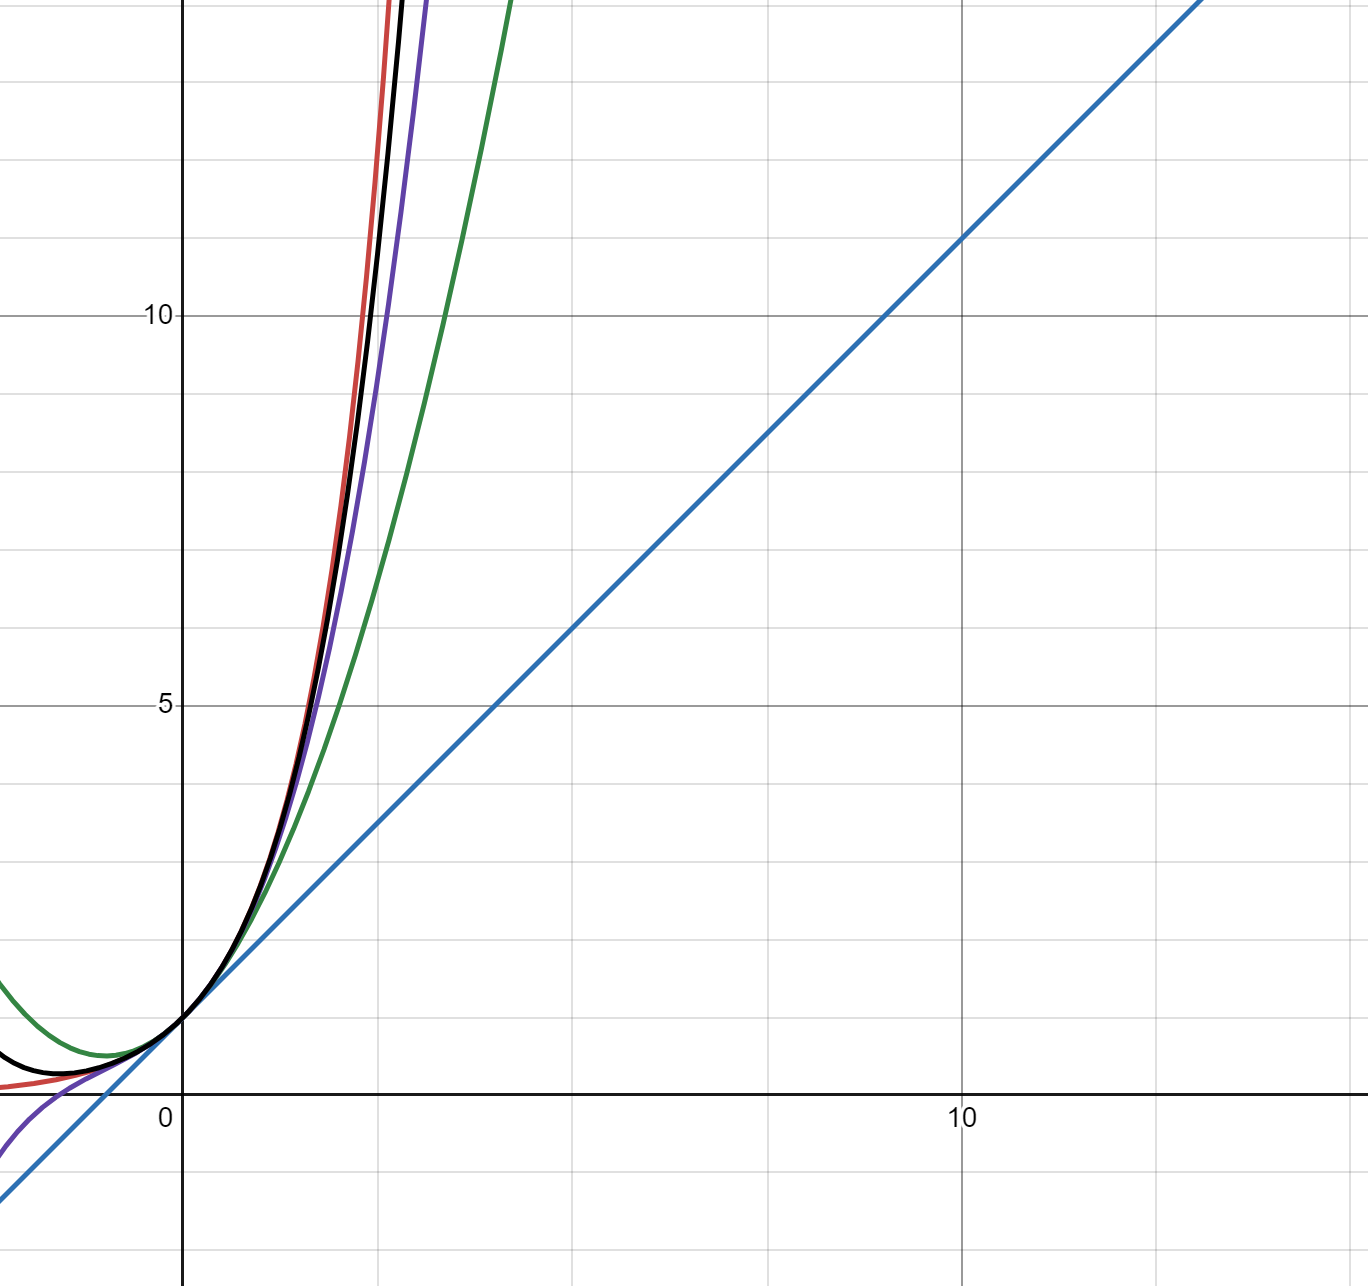
\includegraphics[width=\textwidth]{3.3.png} % 无需重复指定宽度  
\end{myimagebox}     
\caption{\label{fig:3.3}指数函数的$1\sim 5$阶的麦克劳林展开}   
\end{figure}

那么这种泰勒展开得到的多项式$T_n(x)$是否是唯一的?如果读者熟悉线性代数,可以从多项式线性空间的线性性理解这种多项式一定是唯一的,我们介绍下面的定理并且进行证明:
\begin{tcolorbox}[
    colback=bac1,     % 极浅黄色背景
    colframe=fra1,   % 浅黄色边框
    coltitle=white,             % 标题文字白色
    coltext=tex1,
    title=Taylor展开的唯一性,
    fonttitle=\bfseries,        % 标题加粗
arc=3mm,                     % 圆角稍大
breakable
]
设函数$f(x)$在$x_0$的某邻域$O(x_0)$上有定义,且有:
\begin{align*}
    f(x)=c_0+c_1(x-x_0)+...+c_n(x-x_0)^n+o((x-x_0)^n)
\end{align*}

则其中的系数是唯一确定的。
\end{tcolorbox}

我们进行如下的证明:当$x\to x_0$时,右侧变为$c_0$,左侧变为$\lim_{x\to 0}f(x_0)$;然后两面求导,取极限得到$\lim_{x\to x_0}f'(x_0)=\frac{1}{2}c_1$。以此类推,我们发现$c_0,c_1...c_n$的形式与式子3-5的形式是一致的。

然而\textbf{麦克劳林余项}的形式过于粗略,它之说余项是$(x-x_0)^n$的高阶无穷小,但未进一步细化这种余项的形式。利用Lagrange中值定理,我们能得到含拉格朗日余项的泰勒展开:
\begin{tcolorbox}[
    colback=bac1,     % 极浅黄色背景
    colframe=fra1,   % 浅黄色边框
    coltitle=white,             % 标题文字白色
    coltext=tex1,
    title=含拉格朗日余项的泰勒展开,
    fonttitle=\bfseries,        % 标题加粗
arc=3mm,                     % 圆角稍大
breakable
]
设函数$f(x)$在点$x_0$的某邻域$O(x_0)$上$n+1$阶可微,则对每一个$x_0\in O(x_0),x\neq x_0$,在$x_0,x$之间存在$\xi$使得:
\begin{align*}
     f(x)=f(x_0)+f'(x_0)(x-x_0)+...+\frac{f^{(n)}(x_0)(x-x_0)^n}{n!}+\frac{f^{(n+1)}(\xi)}{(n+1)!}(x-x_0)^{n+1}\tag{3-6}
\end{align*}
\end{tcolorbox}

注意与佩亚诺余项不同,拉格朗日余项要求邻域内$n+1$阶可微而不是$n$阶可微。我们对余项反复做Cauchy中值定理,最后一次使用Lagrange中值定理,记余项为$r_n(x)$即有:
\begin{align*}
  \frac{r_n(x)}{(x-x_0)^{n+1}}&=\frac{r_n(x)-r_n(x_0)}{(x-x_0)^{n+1}}=\frac{r'_n(\xi_1)}{(n+1)(\xi_1-x_0)^n}\\
    &=\frac{r'_n(\xi_1)-r'_n(x_0)}{(n+1)(\xi_1-x_0)^{n}}=\frac{r''_n(\xi_2)}{(n+1)n(\xi_2-x_0)^{n-1}}\\
...&=\frac{r^{(n)}_n(\xi_n)-r^{(n)}_n(x_0)}{(n+1)!(\xi_n-x_0)}\\
&=\frac{r^{(n+1)}(\xi)}{(n+1)!} 
\end{align*}

当$x\to 0$时,一些函数的拉格朗日余项的泰勒展开如下,需要读者自行计算证明并记忆:
\begin{tcolorbox}[
    colback=bac2,     % 极浅黄色背景
    colframe=fra2,   % 浅黄色边框
    coltitle=white,             % 标题文字白色
    coltext=tex2,
    title=常用泰勒展开,
    fonttitle=\bfseries,        % 标题加粗
arc=3mm,                     % 圆角稍大
breakable
]
当$x\to 0$时,一些函数的泰勒展开形式如下:
\begin{align*}
  e^x=&1+x+\frac{x^2}{2!}+...+\frac{1}{n!}x^n+\frac{e^\xi}{(n+1)!}x^{n+1}\\&T_n(x)=\sum_{k=0}^n \frac{x^{k}}{k!}\qquad x\in\mathbb{R}\tag{3-7}   
\end{align*}
\begin{align*}
   \sin x=&x-\frac{x^3}{3!}+...+\frac{(-1)^{n-1}}{(2n-1)!}x^{2n-1}+\frac{(-1)^{n}\cos\xi}{(2n+1)!}x^{2n+1}\\&T_n(x)=\sum_{k=1}^{\left \lfloor  (n+1)/2\right \rfloor} \frac{(-1)^{k-1}x^{2k-1}}{(2k-1)!}\qquad x\in\mathbb{R}\tag{3-8}
\end{align*}
\begin{align*}
   \cos x=&1-\frac{x^2}{2}+...+\frac{(-1)^{n}}{(2n)!}x^{2n}+\frac{(-1)^{n+1}\cos\xi}{(2n+2)!}x^{2n+2}\\
&T_n(x)=\sum_{k=0}^{\left \lfloor  n/2\right \rfloor }\frac{(-1)^{k}x^{2k}}{(2k)!}\qquad x\in\mathbb{R}\tag{3-9}
\end{align*}
\begin{align*}
  (1+x)^\alpha =1+\alpha x+\frac{\alpha(\alpha-1)}{2!}x^2...&+\frac{\alpha(\alpha-1)...(\alpha-n+1)}{n!}x^{n}+\frac{\alpha...(\alpha-n)(1+\xi)^{\alpha-n-1}}{(n+1)!}x^{n+1}\\
&T_n(x)=\sum_{k=0}^nC_\alpha^k \frac{x^k}{k!} \qquad x\in(-1,+\infty)\tag{3-10}
\end{align*}
\begin{align*}
   \ln(1+x)=&x-\frac{x^2}{2}+\frac{x^3}{3}...+\frac{(-1)^{n-1}}{n}x^{n}+\frac{(-1)^{n}}{(n+1)(1+\xi)^{n+1}}x^{n+1}\\
&T_n(x)=\sum_{k=1}^n\frac{(-1)^{k-1}x^{k}}{k}\qquad x\in(-1,+\infty)\tag{3-11}
\end{align*}
\end{tcolorbox}

泰勒展开主要分为两种用法:\textbf{第一种是利用已知初等函数的泰勒展开计算复杂函数的泰勒展开;第二种是用泰勒展开细化等价无穷小的思路和计算方法来计算极限}。

\textbf{例:}计算下列函数的Maclaurin展开:
\begin{align*}
    &(1)f(x)=e^{x^2}\qquad (2)f(x)=\arcsin x\\ 
    &(3)f(x)=\sec x \qquad (4)f(x)=\begin{cases}
        \frac{x}{e^x-1}& x\neq 0\\
        1 &x=0
    \end{cases}
\end{align*}

\textbf{解:}(1)将$f(x)=e^x$的泰勒展开中的$x$换成$x^2$即可得到:
\begin{align*}
    e^{x^2}=\sum_{k=0}^{2k}\frac{x^{2k}}{(2k)!}+o(x^{2n})
\end{align*}

为什么可以直接带入而不用就高阶导数计算系数?泰勒展开的形式是唯一的,我们直接带入得到的表达式满足泰勒展开的泰勒多项式的形式,因此就可以肯定我们的表达式是正确的。

(2)我们虽然无法直接展开,但是它的\textbf{导数是可以展开}的:
\begin{align*}
    f'(x)=(1-x^2)^{-\frac{1}{2}}=\sum_{k=0}^{n} C_{-\frac{1}{2}}^k (-1)^kx^{2k}+O(x^{2n})
\end{align*}

然后对其进行积分,并带入$f(0)=0$得到:
\begin{align*}
    \arcsin x=\sum_{k=0}^n\frac{1}{2k+1}\cdot C_{-\frac{1}{2}}^k (-1)^kx^{2k+1}+O(x^{2n+1})
\end{align*}

(3)由于$\sec x$是偶函数,不妨令$x\to 0$时有:
\begin{align*}
    \sec x=c_0+c_2x^2+c_4x^4+...c_{2n}x^{2n}+o(x^{2n+1})
\end{align*}

现在不妨令系数满足:
\begin{align*}
    c_{2n}=(-1)^n\frac{E_{2n}}{(2n)!}
\end{align*}

代入到上式,并且代入$\sec x\cos x\equiv 1$,可以得到数列$\{E_{2n}\}$的递推公式:
\begin{align*}
    & E_0=1\quad E_{2}+E_{0}=1\qquad E_4+\frac{4!}{2!2!}E_2+E_0=0\\
    &E_{2n}+C_{2n}^2 E_{2n-2}+C_{2n}^4E_{2n-4}+...+E_0=0
\end{align*}

因此可以得到$E_2=-1.E_4=5,E_6=-61,E_8=1385...$

(4) 令函数的泰勒展开形式如下:
\begin{align*}
    f(x)=B_0+\frac{B_1}{1!}x+\frac{B_2}{2!}x^2+...+\frac{B_n}{n!}x^n+o(x^n)
\end{align*}

由于函数$f(x)\cdot\frac{e^x-1}{x}\equiv 1$,将左侧的$f(x),\frac{e^x-1}{x}$同时泰勒展开可以得到:
\begin{align*}
    &B_0=1\qquad \frac{1}{2!}B_0+B_1=0\qquad\frac{1}{3!}B_0+\frac{1}{2!1!}B_1+\frac{1}{2!}B_2=0\\
    &C_n^0 B_0+C_n^1 B_1+...C_n^{n-1}B_{n-1}=0
\end{align*}

解得$B_1=-\frac{1}{2},B_2=\frac{1}{6},B_4=-\frac{1}{30}...$并且当$n$是大于1的奇数时$B_n=0$。
\begin{tcolorbox}[
    colback=bac1,     % 极浅黄色背景
    colframe=fra1,   % 浅黄色边框
    coltitle=white,             % 标题文字白色
    coltext=tex1,
    title=小拓展与总结,
    fonttitle=\bfseries,        % 标题加粗
arc=3mm,                     % 圆角稍大
breakable
]
$E_{2n}$被称作\textbf{Euler数},$B_{2n}$被称作\textbf{Bernoulli数}。

计算泰勒展开除了直接带入已知公式外,本题展示了其他办法。可以利用Taylor展开的唯一性和求导/积分后展开的办法进行求解。对于商式$\frac{f(x)}{g(x)}$还可以使用待定系数法,即$f(x)=T_n(x)g(x)$,然后分别展开$f(x),g(x)$求解$T_n(x)$。
\end{tcolorbox}

利用泰勒展开,我们可以进一步丰富等价无穷小的工具,让我们有更多工具计算函数极限。例如计算下面的两个极限:
\begin{align*}
    (1)\lim_{x\to 0}\frac{\frac{x}{1+x}-\ln(1+x)}{x^2}\qquad (2)\lim_{x\to 0}\frac{\cos(\sin x)-\cos x}{x^4}
\end{align*}
\begin{tcolorbox}[
    colback=bac2,     % 极浅黄色背景
    colframe=fra2,   % 浅黄色边框
    coltitle=white,             % 标题文字白色
    coltext=tex2,
    title=一个误区,
    fonttitle=\bfseries,        % 标题加粗
arc=3mm,                     % 圆角稍大
breakable
]
第一题的一种常见错误解法如下,对$\ln(1+x)$使用等价无穷小:
\begin{align*}
    \lim_{x\to 0}\frac{\frac{x}{1+x}-\ln(1+x)}{x^2}= \lim_{x\to 0}\frac{\frac{x}{1+x}-x}{x^2}
= \lim_{x\to 0}\frac{x-(1+x)x}{(1+x)x^2}=1
\end{align*}

实际上错误的原因是因为,$\ln(1+x)=x+o(x)$,而$\lim_{x\to 0}\frac{o(x)}{x^2}$不一定为0,因此对$\ln(1+x)$的等价无穷小展开的不够充分。
\end{tcolorbox}

第一题的正确计算思路如下:
\begin{align*}
    \lim_{x\to 0}\frac{\frac{x}{1+x}-\ln(1+x)}{x^2}&= \lim_{x\to 0}\frac{\frac{x}{1+x}-x-\frac{1}{2}x^2-o(x^2) }{x^2}
\\&= \lim_{x\to 0}\frac{x-(1+x)x-\frac{1}{2}(1+x)x^2 }{(1+x)x^2}=-\frac{1}{2}
\end{align*}

第二题需要把分子展开到$x^4$项,因为只有$\lim_{x\to 0}\frac{o(x^4)}{x^4}=0$,对分子进行展开:
\begin{align*}
    \cos(\sin x)-\cos x&=1-\frac{1}{2!}\sin^2x+\frac{1}{4!}\sin^4x-(1-\frac{1}{2!}x^2+\frac{1}{4!}x^4)+o(x^5)\\
&=-\frac{1}{2}(x-\frac{1}{6}x^3)^2+\frac{1}{24}x^4+\frac{1}{2}x^2-\frac{1}{24}x^4+o(x^5)\\
&=\frac{1}{6}x^4+o(x^5)          
\end{align*}

因此原极限为$\frac{1}{6}$。
\subsection{微分学的应用}
\subsubsection{函数的性质}
我们介绍的第一个问题函数的极值问题,它是指找一个函数在一定范围内的极值和最值问题。我们先对极值进行定义:
\begin{tcolorbox}[
    colback=bac2,     % 极浅黄色背景
    colframe=fra2,   % 浅黄色边框
    coltitle=white,             % 标题文字白色
    coltext=tex2,
    title=极值的定义,
    fonttitle=\bfseries,        % 标题加粗
arc=3mm,                     % 圆角稍大
breakable
]
对于函数$f(x)$若存在$x_0$附近的一个临域$U_\delta(x_0)$,满足:
\begin{align*}
    f(x)\leq f(x_0)\quad or\quad f(x)\geq f(x_0) \qquad \forall x\in U_\delta(x_0)
\end{align*}

前一种情况称$f(x_0)$为\textbf{极大值},$x_0$为\textbf{极大值点}。$f(x_0)$为\textbf{极小值},$x_0$为\textbf{极小值点}。
\end{tcolorbox}

在微分中值定理一章我们介绍了极值点的必要条件——\textbf{Fermat定理},即极值点的导数为0,但这并不是充分条件。例如函数$y=x^3$在$x=0$处导数为0,但是这一点并不是极值点。我们一般把函数的导数为0的点称作\textbf{驻点或稳定点}。极值点要在稳定点中寻找,但是稳定点不都是极值点。

而我们考虑函数$f(x)=x^3,g(x)=x^2$在0的导数,$f'(x)=0,f''(x)=0$。而$g'(x)=0,g''(x)=2$。而$x=0$是函数$f(x)$的稳定点,也是$g(x)$的极小值点。因此我们发现稳定点的二阶导数似乎可以判断极值点的性质。因此我们给出如下结论:
\begin{tcolorbox}[
    colback=bac1,     % 极浅黄色背景
    colframe=fra1,   % 浅黄色边框
    coltitle=white,             % 标题文字白色
    coltext=tex1,
    title=极值点的判定,
    fonttitle=\bfseries,        % 标题加粗
arc=3mm,                     % 圆角稍大
breakable
]
设函数$f(x)$在$(a,b)$有一阶导数,$x_0$是区间内一个稳定点并且$f(x)$在$x_0$处有二阶导数。若$f''(x_0)<0$,则$x_0$是一个极小值点。若$f''(x_0)>0$,则$x_0$是一个极大值点。
\end{tcolorbox}

我们利用Taylor公式进行证明,令$f'(x_0)=0.f''(x_0)>0$,那么:
\begin{align*}
    f(x)&=f(x_0)+\frac{1}{2}f''(x_0)(x-x_0)^2+o((x-x_0)^2)\\
    &=f(x_0)+(\frac{1}{2}f''(x_0)+\alpha(x))(x-x_0)^2
\end{align*}

其中$\alpha(x)$是一个无穷小量。当$x$靠近$x_0$时,第二项与$f''(x_0)$同号,因此$f(x)\geq f(x_0)$。

这个结论可以进一步拓展:
\begin{tcolorbox}[
    colback=bac1,     % 极浅黄色背景
    colframe=fra1,   % 浅黄色边框
    coltitle=white,             % 标题文字白色
    coltext=tex1,
    title=拓展,
    fonttitle=\bfseries,        % 标题加粗
arc=3mm,                     % 圆角稍大
breakable
]
若$f(x)$在$x_0$处有$2n$阶导数,且前$2n-1$阶导数都为0,如果在$x_0$处$2n$阶导数大于0,则$x_0$为极小值点,反之为极大值点。

若$f(x)$在稳定点的前$2n$阶导数为0而$2n+1$阶导数不为0,则$x_0$一定不是极值点。
\end{tcolorbox}

\textbf{例}:说明$x=0$是函数$f(x)=e^x+e^{-x}+2\cos x$的极小值点。
\textbf{解}:计算导数$f'(0)=f''(0)=f'''(0)=0,f^{(4)}(0)=4>0$,根据推论证毕。

接下来我们介绍函数的凹凸性。为了避免混淆,我们把凹性定义为\textbf{下凸性},凸性定义为\textbf{上凸性}。因此我们在这里采用的表述是“函数的凸性”,这和课本的术语有所不同。
\begin{figure} 
\centering     
\renewcommand{\figurename}{图}     
\renewcommand{\thefigure}{3.4}    
\begin{myimagebox}[width=0.5\textwidth] % 直接传入图片尺寸参数      
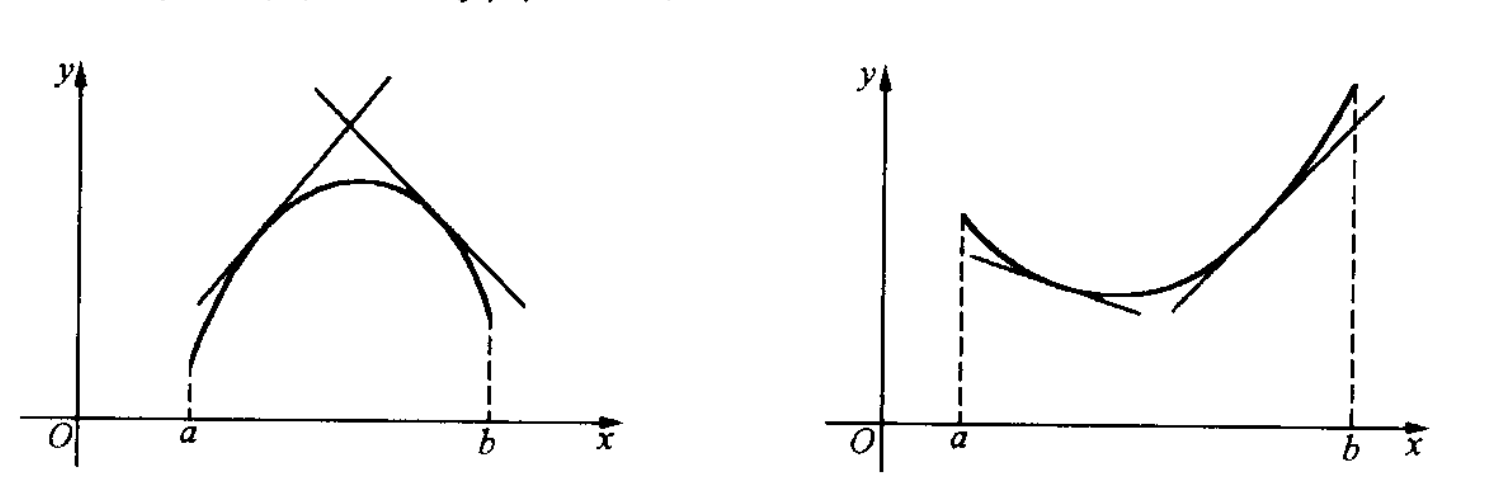
\includegraphics[width=\textwidth]{3.4.png} % 无需重复指定宽度  
\end{myimagebox}     
\caption{\label{fig:3.4}上凸函数和下凸函数}   
\end{figure}

如图3.4就是上凸函数和下凸函数的示意。从几何上理解凹凸性是容易的,但如何用数学语言去刻画这种性质?我们发现对于上凸函数,其函数的切线始终在函数图像的上方,下凸函数则恰好相反。因此我们对函数的凸性进行定义:
\begin{tcolorbox}[
    colback=bac2,     % 极浅黄色背景
    colframe=fra2,   % 浅黄色边框
    coltitle=white,             % 标题文字白色
    coltext=tex2,
    title=函数的凸性,
    fonttitle=\bfseries,        % 标题加粗
arc=3mm,                     % 圆角稍大
breakable
]
若函数$f(x)$在区间$(a,b)$可导,若对于每一点$x_0\in (a,b)$满足:
\begin{align*}
    f(x)<f(x_0)+f'(x_0)(x-x_0)\tag{3-12}
\end{align*}

那么我们称这个函数是一个\textbf{上凸函数}。反之可定义下凸函数。
\end{tcolorbox}

当然如果用这种表述仍然不够直观。我们从函数的凸性出发,可以得到如下的等价定义,而这个定义式判断凹凸性更常用的办法:
\begin{tcolorbox}[
    colback=bac1,     % 极浅黄色背景
    colframe=fra1,   % 浅黄色边框
    coltitle=white,             % 标题文字白色
    coltext=tex1,
    title=二阶导数和函数凹凸性,
    fonttitle=\bfseries,        % 标题加粗
arc=3mm,                     % 圆角稍大
breakable
]
若函数$f(x)$在区间$(a,b)$有二阶导数,若对每一点$x_0$都\textbf{有$f''(x)>0$},则函数是\textbf{下凸函数}。反之是上凸函数。
\end{tcolorbox}

这个定理的证明如下,使用带拉格朗日余项的泰勒公式,则有:
\begin{align*}
    f(x)=f(x_0)+f'(x_0)(x-x_0)+\frac{f''(\xi)}{2}(x-x_0)^2
\end{align*}

若$f''(x)>0$,则$f(x)>f(x_0)+f'(x_0)(x-x_0)$,满足函数上凸的定义。\textbf{接下来我们会继续介绍函数凸性的等价定义和定理,这部分内容读者可自行跳过}。

\begin{tcolorbox}[
    colback=bac2,     % 极浅黄色背景
    colframe=fra2,   % 浅黄色边框
    coltitle=white,             % 标题文字白色
    coltext=tex2,
    title=函数凸性的等价定义,
    fonttitle=\bfseries,        % 标题加粗
arc=3mm,                     % 圆角稍大
breakable
]
设函数$f(x)$在区间$I$上有定义,若对$\forall x_1,x_2\in I,x_1\neq x_2,\forall \lambda \in (0,1)$,下面不等式成立:
\begin{align}
    f(\lambda x_1+(1-\lambda)x_2)>\lambda f(x_1)+(1-\lambda)f(x_2)\tag{3-13}
\end{align}

则称函数$f(x)$为上凸函数。
\end{tcolorbox}

这个定义的证明过程如下,我们将3-12的不等式右侧移到左侧,然后使用拉格朗日中值定理:
\begin{align*}
    f(x)-f(x_0)-f'(x_0)(x-x_0)=[f'(\xi)-f'(x_0)](x-x_0)<0
\end{align*}

不妨令$x>x_0$,因此$f'(\xi)<f'(x_0)$,也就是说$f'(x)$是单调递减的,根据二阶导数和函数凸性的关系证毕。

函数凸性的另一个表达形式如下:
\begin{tcolorbox}[
    colback=bac1,     % 极浅黄色背景
    colframe=fra1,   % 浅黄色边框
    coltitle=white,             % 标题文字白色
    coltext=tex1,
    title=函数凸性定理,
    fonttitle=\bfseries,        % 标题加粗
arc=3mm,                     % 圆角稍大
breakable
]
函数$f(x)$在区间$I$是下凸函数的充要条件是$\forall x_1,x_2,x_3\in I,x_1<x_2<x_3$,下面的式子成立:
\begin{align*}
    \frac{f(x_2)-f(x_1)}{x_2-x_1}<\frac{f(x_3)-f(x_1)}{x_3-x_1}<\frac{f(x_3)-f(x_2)}{x_3-x_2}\tag{3-14}
\end{align*}
\end{tcolorbox}

我们利用3-13的定义证明必要性。记$\lambda=\frac{x_3-x_2}{x_3-x_1}$,那么$0<\lambda<1,x_2=\lambda x_1+(1-\lambda)x_3$。由于$f(x)$下凸,则:
\begin{align*}
    f(x_2)&<\lambda f(x_1)+(1-\lambda)f(x_3)\\
    (x_3-x_1)[f(x_2)-f(x_1)]&<(x_2-x_1)[f(x_3)-f(x_1)]
\end{align*}

充分性请读者自己证明留作思考。

若函数$f(x)$在某一点$x_0$附近的凸性不一致,则称这一点是\textbf{拐点}。对于有连续二阶导数的函数$f(x)$(记作$f(x)\in C^2[a,b]$),拐点二阶导数为0。
\begin{figure}[H] 
\centering     
\renewcommand{\figurename}{图}     
\renewcommand{\thefigure}{3.5}    
\begin{myimagebox}[width=0.3\textwidth] % 直接传入图片尺寸参数      
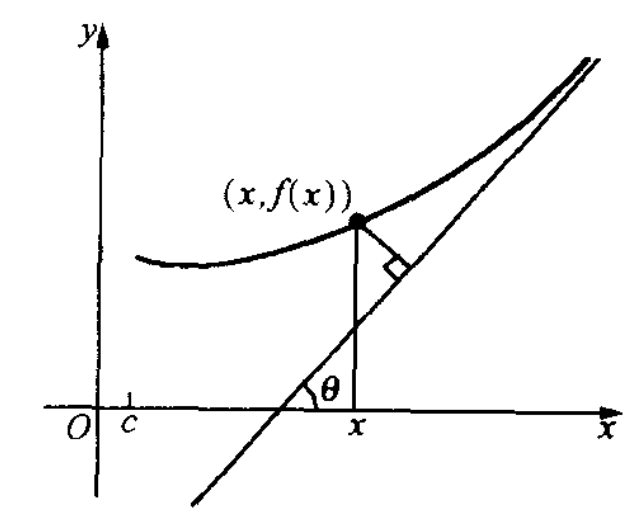
\includegraphics[width=\textwidth]{3.5.png} % 无需重复指定宽度  
\end{myimagebox}     
\caption{\label{fig:3.5}函数的渐进线}   
\end{figure}

接下来我们介绍函数的渐进线,如图3.5所示。
\begin{tcolorbox}[
    colback=bac2,     % 极浅黄色背景
    colframe=fra2,   % 浅黄色边框
    coltitle=white,             % 标题文字白色
    coltext=tex2,
    title=渐近线,
    fonttitle=\bfseries,        % 标题加粗
arc=3mm,                     % 圆角稍大
breakable
]
设函数$f(x)$定义在$[c,+\infty)$上,如果当$x\to\infty$时函数到直线$y=ax+b$的距离趋近于0,称这条直线为\textbf{渐近线}。渐近线存在的充要条件是下面两个极限存在并且:
\begin{align*}
    a=\lim_{x\to\infty}\frac{f(x)}{x}\qquad b=\lim_{x\to\infty}(f(x)-ax)
\end{align*}
\end{tcolorbox}

\subsubsection{不等式(选学)}
在第一章中我们介绍了一些基本不等式,这些不等式的证明正是利用了函数求导,判断单调性与零点等办法。这里我们对讲过的不等式不再介绍,而是介绍一些其他不等式,主要是强调对微分学和函数性质的进一步应用。

我们先介绍下凸函数的Jensen不等式,其公式内容可以理解为3-13定义的拓展版,形式一致:

\begin{tcolorbox}[
    colback=bac1,     % 极浅黄色背景
    colframe=fra1,   % 浅黄色边框
    coltitle=white,             % 标题文字白色
    coltext=tex1,
    title=下凸函数的Jensen不等式,
    fonttitle=\bfseries,        % 标题加粗
arc=3mm,                     % 圆角稍大
breakable
]
设函数$f(x)$是区间$I$上的二阶可微下凸函数,则$\forall x_1,x_2...x_n\in I$与满足条件的$\lambda_1+\lambda_2+...+\lambda_n=1$的$n$个正数,下列不等式成立:
\begin{align*}
    \lambda_1f(x_1)+\lambda_2f(x_2)+...+\lambda_nf(x_n)\geq f(\lambda_1x_1+...+\lambda_nx_n)\tag{3-15}
\end{align*}

当$x_1=x_2=...x_n$时等号成立。
\end{tcolorbox}

我们不妨令$\lambda_1x_1+...\lambda_nx_n=x_0$。那么对于任意的$f(x_i)$可以写出在$x_0$展开的带拉格朗日余项的泰勒公式:
\begin{align*}
    f(x_i)=f(x_0)+f'(x_0)(x-x_0)+\frac{f''(\xi)}{2}(x-x_0)^2
\end{align*}

因此对于3-15左侧的$\sum\lambda_if(x_i)$,可以写作:
\begin{align*}
\sum_{i=1}^n\lambda_if(x_i)&=\sum_{i=1}^n\lambda_i\left[f(x_0)+f'(x_0)(x_i-x_0)+\frac{f''(\xi)}{2}(x_i-x_0)^2 \right]\\
    &=\sum_{i=1}^n\lambda_i\cdot f(x_0)+f'(x_0)\sum_{i=1}^n\left[\lambda_i(x_i-x_0)\right]+\frac{f''(\xi)}{2}\sum_{i=1}^n\left[\lambda_i(x_i-x_0)^2\right]\\
 &\geq f(x_0)+f'(x_0)(x_0-x_0)=f(x_0)
\end{align*}

Jensen不等式在证明其他函数不等式有着非常重要的应用,例如下面对算术平均值——几何平均值不等式的推广:
\begin{tcolorbox}[
    colback=bac1,     % 极浅黄色背景
    colframe=fra1,   % 浅黄色边框
    coltitle=white,             % 标题文字白色
    coltext=tex1,
    title=算术平均值——几何平均值不等式的推广,
    fonttitle=\bfseries,        % 标题加粗
arc=3mm,                     % 圆角稍大
breakable
]
设有非负数$x_1,x_2...x_n$和正数$\lambda_1,\lambda_2..\lambda_n$,且$\lambda_1+\lambda_2+...+\lambda_n=1$。则下列不等式成立:
\begin{align*}
    \prod_{k=1}^n x_k^{\lambda_k}\leq \sum_{k=1}^n\lambda_kx_k\tag{3-16}
\end{align*}

当$x_1=x_2=...x_n$时等号成立。
\end{tcolorbox}

由于左边是一个连乘的形式,我们把不等式两侧取对数,即证明:
\begin{align*}
 \lambda_k \ln x_k\leq \ln(\sum_{k=1}^n\lambda_kx_k)
\end{align*}

接下来考虑函数$f(u)=-\ln u$,由于函数的二阶导数大于0,因此函数是下凸函数,利用Jenson不等式则有:
\begin{align*}
    \sum_{k=1}^n\lambda_k(-\ln u_k)\geq -\ln (\sum_{k=1}^n \lambda_ku_k)
\end{align*}

消去符号,结论证毕。

\begin{tcolorbox}[
    colback=bac1,     % 极浅黄色背景
    colframe=fra1,   % 浅黄色边框
    coltitle=white,             % 标题文字白色
    coltext=tex1,
    title=H\"older 不等式,
    fonttitle=\bfseries,        % 标题加粗
arc=3mm,                     % 圆角稍大
breakable
]
设$x_1,x_2,...x_n;y_1,y_2...y_n$都是非负实数,且$p>1,q>1,\frac{1}{p}+\frac{1}{q}=1$($p,q$满足共轭条件),则:
\begin{align*}
    \sum_{k=1}^n x_ky_k\leq \left(\sum_{k=1}^n x_k^p\right)^{1/p}\cdot \left(\sum_{k=1}^n y_k^q\right)^{1/q}\tag{3-17}
\end{align*}

等号成立的充要条件是$x_1^p,x_2^p...x_n^p$与$y_1^q,y_2^q...y_n^q$成比例。
\end{tcolorbox}

我们先对至少有一个数组中每个数都大于0的情况进行证明。不妨令$y_1,y_2...y_n>0$。则我们先取辅助下凸函数,令$f(u)=u^p (u\geq 0)$。那么二阶导数是大于0的。接下来我们要使用Jenson不等式,我们令$\lambda_k$和$u_k$的参数满足:
\begin{align*}
    \lambda_k=\frac{y_k^q}{\sum_{i=1}^n y_i^q}\qquad u_k=x_ky_k^{1-q}
\end{align*}

代入Jenson不等式,则不等式左侧为:
\begin{align*}
\sum_{k=1}^n\lambda_kf(u_k)&=\frac{\sum_{k=1}^ny_k^q\cdot(x_ky_k^{1-q})^p}{\sum_{i=1}^n y_i^q}=\frac{\sum_{i=1}^n x_i^p}{\sum_{i=1}^n y_i^q}
\end{align*}

不等式右侧变为:
\begin{align*}
   f(\sum_{k=1}^n\lambda_ku_k)=\left[\sum_{k=1}^n\frac{y_k^q\cdot x_ky_k^{1-q}}{\sum_{i=1}^n y_i^q}\right]^p
=\left(\frac{\sum_{k=1}x_ky_k}{\sum_{i=1}^ny_k^q} \right)^p
\end{align*}

代入Jenson不等式,化简后定理证毕。若两个数组有部分数为0,可以先把这些带0的数剔除,然后归结到前面的情况。

\begin{tcolorbox}[
    colback=bac1,     % 极浅黄色背景
    colframe=fra1,   % 浅黄色边框
    coltitle=white,             % 标题文字白色
    coltext=tex1,
    title=Minkowski不等式,
    fonttitle=\bfseries,        % 标题加粗
arc=3mm,                     % 圆角稍大
breakable
]
设$x_1,x_2,...x_n;y_1,y_2...y_n$都是非负实数,且$p>1$。则下面不等式成立:
\begin{align*}
    \left[\sum_{k=1}^n (x_k+y_k)^p\right]^{1/p}\leq (\sum_{k=1}^n x_k^p)^{1/p}\cdot (\sum_{k=1}^n y_k)^{1/p}
\end{align*}

当数组成比例时,等号成立。
\end{tcolorbox}

我们继续构造下凸辅助函数$f(u)=(1-u^p)^{1/p},0<u<1$,其二阶导数是大于0的。令:
\begin{align*}
    \lambda_k=\frac{(x_k+y_k)^p}{\sum_{i=1}^n(x_i+y_i)^p}\qquad u_k=(\frac{x_k}{x_k+y_k})^p
\end{align*}

代入到Jenson不等式中,化简得到:
\begin{align*}
    \left[1-(\sum_{k=1}^n\frac{x)k^p}{\sum_{i=1}^n(x_i+y_i)^p})^{1/p}\right]^p\leq \frac{\sum_{k=1}^n y_k^p}{\sum_{k=1}^n(x_k+y_k)^p}
\end{align*}

两边开$p$次根加以整理即可。

\subsection{习题补充与拓展}
\textbf{例1}:(1)设函数$f(x)$在$[0,+\infty)$可微,且$0\leq f(x)\leq\frac{x}{(1+x)^2}$,证明$\exists \xi>0$使得下式成立:
\begin{align*}
    f'(\xi)=\frac{1-\xi^2}{(1+\xi^2)^2}
\end{align*}

(2)设函数$f(x)$在$[a,b]$连续且在$(a,b)$可微,证明存在$\xi,\eta\in(a,b)$,使得:
\begin{align*}
    \frac{f'(\xi)}{f'(\eta)}=\frac{e^b-e^a}{b-a}e^{-\eta}
\end{align*}

\textbf{解}:(1)不妨构造辅助函数$F(x)=f(x)-\frac{x}{(1+x)^2}$。当$x\to \infty$时,由于$\lim_{x\to\infty}\frac{x}{(1+x)^2}=0$,根据夹逼定理可以得到$\lim_{x\to\infty}f(x)=0$,因此$\lim_{x\to\infty}F(x)=0$。根据Rolle定理推论,$F'(\xi)=0$,化简后证毕。

(2)这个问题的迷惑点在于它长得像Cauchy中值定理但完全没有关系。首先我们对$f(x)$使用拉格朗日中值定理,则$(b-a)f'(\xi)=f(b)-f(a)$,因此两边同除可以得到:
\begin{align*}
    \frac{f(b)-f(a)}{(b-a)(e^b-e^a)}=\frac{f'(\xi)}{e^b-e^a}
\end{align*}

另一方面我们看上面的式子,如果分母把$b-a$提取出去,剩下的部分可以用Cauchy中值定理,即:
\begin{align*}
    \frac{f(b)-f(a)}{(b-a)(e^b-e^a)}=\frac{1}{b-a}\cdot\frac{f(b)-f(a)}{e^b-e^a}=\frac{f(\eta)}{b-a}e^{-\eta}
\end{align*}

两式联立可以得到结论。

\textbf{例2}:设函数$f(x)$在$[0,1]$连续且在$(0,1)$可微,$f(0)=f(1)=0,f(\frac{1}{2})=1$,证明:

(1)存在$\eta\in(\frac{1}{2},1)$使得$f(\eta)=\eta$

(2)对任何实数$\lambda$,$\exists \xi\in (0,\eta)$,使得:
\begin{align*}
    f'(\xi)-\lambda[f(\xi)-\xi]=1
\end{align*}

\textbf{解}:(1)构造辅助函数$F(x)=f(x)-x$,由题目条件$F(\frac{1}{2})>0,F(1)<0$,根据介值定理证毕。

(2)构造辅助函数$G(x)=[f(x)-x]e^{-\lambda x}$,由题目条件$G(0)=0,G(\eta)=0$,使用Rolle定理证毕。

\textbf{例3}:计算$f(x)=\frac{\arcsin x}{\sqrt{1-x^2}}$带Peano余项的Maclaurin公式。

\textbf{解}:我们采用\textbf{待定系数法}。不妨令函数$f(x)$的Taylor展开为:
\begin{align*}
    f(x)=a_0+a_1x+...+a_nx^n+o(x^n)=\sum_{k=0}^n a_kx^k+o(x^n)
\end{align*}

我们将$f(x)$的分母乘到右边并对两边求导:
\begin{align*}
\arcsin x&=\sqrt{1-x^2}\sum_{k=0}^n a_kx^k \\
\frac{1}{\sqrt{1-x^2}}&=-\frac{x}{\sqrt{1-x^2}} \sum_{k=0}^n a_kx^k+\sqrt{1-x^2}\sum_{k=0}^{n}(k+1)a_{k+1}x^k   
\end{align*}

进一步同乘分母,化简得到:
\begin{align*}
&-x\sum_{k=0}^n a_kx^k+(1-x^2)\sum_{k=0}^{n}(k+1)a_{k+1}x^k  =1\\
&\sum_{k=0}^n(k+1)a_{k+1}x^k-\sum_{k=2}^n(k-1)a_{k-1}x^k-\sum_{k=1}^na_{k-1}x^k=1
\end{align*}

接下来比较系数,由$f(0)=0$得到$a_0=0$,$n=0$时$a_1=1$。当$n\geq 2$时,根据题目关系:
\begin{align*}
    (n+1)a_{n+1}-(n-1)a_{n-1}-a_{n-1}=0\qquad a_{n+1}=\frac{n}{n+1}a_{n-1}
\end{align*}

由于$a_0=0$,对于偶数情况下系数都是0,而对于奇数可计算得到:
\begin{align*}
    a_{2k+1}=\frac{2^kk!}{(2k+1)!!}=\frac{4^k(k!)^2}{(2k+1)!}
\end{align*}

\textbf{例4:}(1)设函数$f(x)$在$(0,+\infty)$上二阶可微,且已知$M_0$为$|f(x)|$的最大值,$M_2$为$|f''(x)|$最大值且都是有限数。证明$|f'(x)|$的最大值$M_1$也是有限数,并且有$M_1\leq 2\sqrt{M_0M_2}$。

(2)设函数$f(x)$在$[a,b]$上二阶可微,且$f'(a)=f'(b)=0$,证明$\exists \xi\in(a,b)$使得:
\begin{align*}
    |f''(\xi)|\geq \frac{4}{(b-a)^2}|f(b)-f(a)|
\end{align*}

\textbf{解:}(1)对函数在$[x,x+t]$上Taylor展开:
\begin{align*}
    f(x+t)=f(x)+f'(x)t+\frac{f''(\xi)}{2}t^2\qquad \xi\in(x,x+t)
\end{align*}

因此对$f'(x)$进行估计:等式右侧其他项移到左边,并取绝对值:
\begin{align*}
    |tf'(x)|&=|f(x+t)-f(x)-\frac{t^2}{2}f''(\xi)|\\
    &\leq |f(x+t)|+|f(x)|+\frac{t^2}{2}|f''(\xi)|\\
    &\leq 2M_0+\frac{t^2}{2}M_2
\end{align*}

因此可以得到对于每一个$x$和每一个$t$都有:
\begin{align*}
    |f'(x)|\leq \frac{2M_0}{t}+\frac{t}{2}M_2
\end{align*}

由于不等式恒成立,因此左边可以取到最大值,右边可以取到最小值,因此$M_1\leq 2\sqrt{M_0M_2}$证毕。

(2)我们分别在$x=a,x=b$两处使用泰勒展开:
\begin{align*}
    f(x)&=f(a)+\frac{f''(\xi)}{2}(x-a)^2\qquad \xi\in(a,x)\\
    f(x)&=f(b)+\frac{f''(\eta)}{2}(b-x)^2\qquad  \eta\in(x,b)
\end{align*}

在上面的式子中令$x=\frac{a+b}{2}$可得:
\begin{align*}
 f(x)=f(a)+\frac{f''(\xi)}{2}\frac{(b-a)^2}{4}
=f(b)+\frac{f''(\eta)}{2}\frac{(b-a)^2}{4}
\end{align*}

两式相减可得:
\begin{align*}
f(b)-f(a)&=\frac{(b-a)^2}{8} (f''(\xi)-f''(\eta))\\
\frac{8}{(b-a)^2} |f(b)-f(a)|&=|f''(\xi)-f''(\eta)|\leq|f''(\xi)|+|f''(\eta)|
\end{align*}

则$f''(\xi)$和$f''(\eta)$至少有一个大于不等式左侧的一半,证毕。

\textbf{例5}:(1)设当$x\in[0,a]$时,有$|f''(x)|\leq M$,并且$f(x)$在$(0,a)$中取到最大值,证明$|f'(0)|+|f'(a)|\leq Ma$

(2)设函数$f(x)$在$[0,1]$上可微,且$f(0)=0,f(x)\neq 0,\forall x\in(0,1)$。证明对每一个$\alpha>0$,都存在$\xi\in(0,1)$成立:
\begin{align*}
    \alpha\cdot\frac{f'(\xi)}{f(\xi)}=\frac{f'(1-\xi)}{f(1-\xi)}
\end{align*}

\textbf{解}:(1)设函数在$x_0$处取得最大值,则$f'(x_0)=0$,因此对$f'(x)$使用拉格朗日中值定理,存在$\xi_1\in(0,x_0),\xi_2\in(x_0,a)$有:
\begin{align*}
    f''(\xi_1)=\frac{f'(x_0)-f'(0)}{x_0}\qquad f''(\xi_2)=\frac{f'(a)-f'(x_0)}{(a-x_0)}
\end{align*}

因此$f'(0)=-x_0f''(\xi_1),f'(a)=(a-x_0)f''(\xi_2)$。因此原不等式可以化作:
\begin{align*}
    |f''(0)|+|f''(a)|=x_0|f''(\xi_1)|+(a-x_0)|f''(\xi_2)|\leq x_0M+(a-x_0)M=Ma
\end{align*}

(2)构造函数$g(x)=f(x)^\alpha f(1-x)$,并且$g(0)=g(1)=0$,接下来对$g(x)$求导:
\begin{align*}
g'(x)&=\alpha f(x)^{\alpha-1}f'(x)f(1-x)-f(x)^\alpha f'(1-x)\\
&=f(x)^\alpha f(1-x)\cdot\left(\alpha \frac{f'(x)}{f(x)}-\frac{f'(1-x)}{f(1-x)}\right)
\end{align*}

因此对$g(x)$使用Rolle定理,$g'(\xi)=0$,化简得到题目结果。

\textbf{例6}:(1)设函数$f(x)$在实数域上二阶连续可微,且$|f(x)|\leq 1$,且$[f'(0)]^2+[f(0)]^2=4$,证明存在$\xi$使得$f(\xi)+f''(\xi)=0$。

(2)设函数$f(x)$在$(a.b)$上任意阶可微,且对于每个正整数$n$都有$f^{(n)}(x)\geq 0$ 且$|f(x)|\leq M$。证明对每个$x\in(a,b),r>0.x+r\in(a,b)$,下面的式子成立:
\begin{align*}
    f^{(n)}(x)\leq \frac{2Mn!}{r^n}\qquad \forall n\in\mathbb{N^+}
\end{align*}

\textbf{解}:(1)根据拉格朗日中值定理,$\exists \xi_1\in(-2,0),\xi_2\in(0,2)$。使得:
\begin{align*}
    f'(\xi_1)=\frac{f(0)-f(-2)}{2}\qquad f'(\xi_2)=\frac{f(2)-f(0)}{2}
\end{align*}

所以可以得到$|f'(\xi_1)|\leq 1,|f'(\xi_2)|\leq 1$设$g(x)=(f(x))^2+(f'(x))^2$,则$g'(x)=2f'(x)[f(x)+f''(x)]$,由于$|f'(xi_1)|\leq 1,|f'(\xi_2)|\leq 1$,因此$g(\xi_1),g(\xi_2)\leq 2$。而$g(0)=4$,因此在$(\xi_1,\xi_2)$上有最大值。设最大值在$x=\xi$取到,则$g'(\xi)=0$,而$g'(\xi)\geq g(0)=4$,则$|f'(\xi)|\geq\sqrt{3}\neq 0$,因此$g'(\xi)=0$必有$f(\xi)+f''(\xi)=0$。

(2)根据Taylor公式可以得到:
\begin{align*}
    f(x+r)&=\sum_{k=0}^n f^{(k)}(x)r^k+\frac{f^{(n+1)}(x+\theta r)}{(n+1)!}r^{n+1}\\
    &\geq f(x)+\frac{f^{(n)}(x)}{n!}r^n
\end{align*}

所以有:
\begin{align*}
    f^{(n)}(x)\leq \frac{[f(x+r)-f(x)]n!}{r^n}\leq\frac{2Mn!}{r^n}
\end{align*}

\textbf{例7:}计算下列极限,第四题中$x\geq 2$为一常数。
\begin{align*}
&(1) \lim_{n\to\infty}n^2\ln(n\sin\frac{1}{n})\qquad \qquad(2)\lim_{n\to\infty}(-1)^n n\sin(\sqrt{n^2+2}\pi)\\
&(3)\lim_{x\to 0}\frac{x\sin(\sin x)-\sin^2x}{x^6}\qquad (4) \lim_{n\to\infty}n^x\left[(1+\frac{1}{n+1})^{n+1} -(1+\frac{1}{n})^n 
\right] 
\end{align*}

\textbf{解:}(1)利用等价无穷小和Taylor展开:
\begin{align*}
n^2\ln(n\sin\frac{1}{n})&\sim n^2\cdot(n\sin\frac{1}{n}-1)\sim n^2(-\frac{1}{6n^2}+o(\frac{1}{n^3}))\to -\frac{1}{6}    
\end{align*}

(2)利用诱导公式$\sin(x-n\pi)=(-1)^n\sin x$可以得到:
\begin{align*}
(-1)^n n\sin(\sqrt{n^2+2}\pi)&=n\sin(\sqrt{n^2+2}\pi-n\pi)=n\sin\frac{2\pi}{\sqrt{n^2+2}+n } \\
&\sim \frac{2n\pi}{\sqrt{n^2+2}+n}=\pi    
\end{align*}

(3)直接使用$\sin x$的展开:
\begin{align*}
\frac{x\sin(\sin x)-\sin^2x}{x^6}&\sim\frac{x\sin\left[x-\frac{x^3}{6}+o(x^3)\right]
-\left[x-\frac{x^3}{6}+o(x^3)\right]^2}{x^6}\\
  &\sim \frac{x\left[(x-\frac{x^3}{6})-\frac{1}{6} (x-\frac{x^3}{6})^3\right]- 
(x-\frac{x^3}{6})^2}{x^6}  \\
&\sim \frac{\frac{1}{18}x^6+o(x^6) }{x^6}\to\frac{1}{18}  
\end{align*}

(4)使用指对变换:
\begin{align*}
n^x\left[(1+\frac{1}{n+1})^{n+1} -(1+\frac{1}{n})^n \right]&=n^x\left[\exp
\left[(n+1)\ln(1+\frac{1}{n+1})\right]-\exp
\left[n\ln(1+\frac{1}{n})\right]\right] \\
&= n^x \exp n\ln(1+\frac{1}{n})\cdot \left[\exp
\left[(n+1)\ln(1+\frac{1}{n+1})- n\ln(1+\frac{1}{n})\right]-1\right] \\
&\sim en^x\cdot \left[(n+1)\ln(1+\frac{1}{n+1})-n\ln(1+\frac{1}{n}) \right]\\
&\sim en^x[-\frac{1}{2(n+1)}+\frac{1}{2n}]\\
&\sim \frac{e}{2n^{x-2}} 
\end{align*}

当$x=2$时极限为$e$,反之极限为$0$。

\textbf{例8}:(1)设$f''(a)$存在,证明:
\begin{align*}
    \lim_{h\to 0}\frac{f(a+2h)-2f(a+h)+f(a)}{h^2}=f''(a)
\end{align*}

(2)设函数$f(x)$在$[0,+\infty)$上二阶连续可微,且$f''(x)>0,f(0)=f'(0)=0$,求极限$\lim_{x\to 0+}\frac{xf(u)}{uf(x)}$,其中$u$是函数$f(x)$图象在点$(x,f(x))$处切线在$x$轴上的截距。

\textbf{解:}(1)根据Taylor公式有:
\begin{align*}
    f(a+h)&=f(a)+f'(a)h+f''(a)\frac{h^2}{2}+o(h^2)\\
    f(a+2h)&=f(a)+2f'(a)h+2f''(a)h^2+o(h^2)
\end{align*}

带入到要计算的极限就可得到结论。

(2)首先要把$u$表示出来,由于切线表达式为$y-f(x_0)=f'(x_0)(x-x_0)$,所以$u$的表达式为:
\begin{align*}
    u=x-\frac{f(x)}{f'(x)}
\end{align*}

把函数$f(u)$在0处展开,利用拉格朗日余项:
\begin{align*}
    f(u)=f(0)+f'(0)u+\frac{f''(\xi)u^2}{2}=\frac{f''(\xi)}{2}u^2
\end{align*}

因此代入上式得到:
\begin{align*}
    \frac{xf(u)}{uf(x)}=\frac{xu}{2}\cdot\frac{f''(\xi)}{f(x)}=\frac{f''(\xi)}{2}\left[\frac{x^2}{f(x)}-\frac{x}{f'(x)}\right]
\end{align*}

当$x\to\infty$时,由于$u\to 0$,利用洛必达:
\begin{align*}
    \left[\frac{x^2}{f(x)}-\frac{x}{f'(x)}\right]\to \frac{2}{f''(0)}-\frac{1}{f''(0)}=\frac{1}{f''(0)}
\end{align*}

而当$x\to 0$时,$f''(\xi)\to f''(0)$,所以原式极限为$\frac{1}{2}$。

\section{不定积分}
\subsection{不定积分的定义和性质}
\subsubsection{不定积分的定义}
前三章的内容侧重于微分学,接下来我们用两章内容介绍积分学的基本内容。积分学主要分为不定积分和定积分两章。要注意\textbf{定积分和不定积分的本质是不一样的,而二者是根据Newton-Leibniz法则联系在一起的}。定积分的积分形式和定义有很多,我们重点介绍的是Riemann积分。

\textbf{不定积分的定义是源于求导的逆运算而定积分不是}。求不定积分的本质在于对于给定函数$f(x)$,求出所有的函数$F(x)$使得$F'(x)=f(x)$。我们把$F(x)$称作\textbf{原函数}。

为什么我们说的是“\textbf{所有的函数}”?我们思考如果一个函数$F(x)$是$f(x)$的原函数,那么$F(x)+C$也是$f(x)$的原函数,也就是说$G(x)=F(x)+C$也是$f(x)$的原函数,而原函数的这个表达式就被称作\textbf{不定积分}。记作$G(x)=\int f(x)\mathrm{d}x$。

利于$\cos x$,其是从$\sin x$求导过来的,因此$\cos x$的不定积分为:
\begin{align*}
    \int \cos x\mathrm{d}x=\sin x+C
\end{align*}

\begin{tcolorbox}[
    colback=bac1,     % 极浅黄色背景
    colframe=fra1,   % 浅黄色边框
    coltitle=white,             % 标题文字白色
    coltext=tex1,
    title=基本积分表,
    fonttitle=\bfseries,        % 标题加粗
arc=3mm,                     % 圆角稍大
breakable
]
事实上,由于不定积分是求导的逆运算,我们根据导数表可以得到基本积分表:
\begin{align*}
&\int x^\alpha\mathrm{d}x=\frac{1}{\alpha+1}x^{\alpha+1}+C\qquad (\alpha\neq 1)\tag{4-1}\\
 &\int \cos x\mathrm{d}x=\sin x+C\quad \int \sin x\mathrm{d}x=-\cos x+C\tag{4-2}\\
&\int \frac{\mathrm{d}x}{\sqrt{1-x^2}}=\arcsin x+C\quad \int\frac{\mathrm{d}x}{1+x^2}=\arctan x+C\tag{4-3}\\
&\int a^x\mathrm{d}x=\frac{a^x}{\ln a}+C (a>0,a\neq 1)\quad \int\frac{1}{x}\mathrm{d}x=\ln|x|+C\tag{4-4}       
\end{align*}
\end{tcolorbox}

初等函数的不定积分不一定是初等函数,如果原函数不是初等函数,我们称函数不可积。
\subsubsection{不定积分的性质}
不定积分具有\textbf{线性性},也就是说:
\begin{align*}
    \int [f(x)+g(x)]\mathrm{d}x&=\int f(x)\mathrm{d}x+\int g(x)\mathrm{d}x\\
    \int cf(x)\mathrm{d}x&=c\int f(x)\mathrm{d}x
\end{align*}

对于原函数存在三个基本问题:存在性,唯一性,如何求。对于存在性要放在定积分一章讲述,如何求在不定积分的计算中讲述。在这里我们介绍原函数形式唯一性。

\begin{tcolorbox}[
    colback=bac2,     % 极浅黄色背景
    colframe=fra2,   % 浅黄色边框
    coltitle=white,             % 标题文字白色
    coltext=tex2,
    title=不定积分原函数形式唯一性,
    fonttitle=\bfseries,        % 标题加粗
arc=3mm,                     % 圆角稍大
breakable
]
设函数$F(x),G(x)$都是$f(x)$在区间$I$上的原函数,则一定有:
\begin{align*}
    F(x)=G(x)+C
\end{align*}

这个定理的证明也很简单,构造辅助函数$M(x)=F(x)-G(x)$,求导即可。
\end{tcolorbox}

\subsection{不定积分的计算}
\subsubsection{不定积分换元法}
如果只根据基本积分表计算不定积分,我们可计算的积分数量非常有限。因此不定积分换元法和分部积分法是我们计算不定积分的核心工具。接下来我们介绍不定积分的换元法:
\begin{tcolorbox}[
    colback=bac1,     % 极浅黄色背景
    colframe=fra1,   % 浅黄色边框
    coltitle=white,             % 标题文字白色
    coltext=tex1,
    title=不定积分第一换元法,
    fonttitle=\bfseries,        % 标题加粗
arc=3mm,                     % 圆角稍大
breakable
]
设函数$F'(y)=f(y)$,且$y=\varphi(x)$可导,由复合函数求导公式得到:
\begin{align*}
    \frac{\mathrm{d}}{\mathrm{d}x}F(\varphi(x))=f(\varphi(x))\varphi'(x)
\end{align*}

于是就有:
\begin{align*}
    \int f(\varphi(x))\mathrm{d}(\varphi(x))=F(\varphi(x))+C
\end{align*}
\end{tcolorbox}

\textbf{例:}计算积分
\begin{align*}
    (1)\int \tan x\mathrm{d}x\qquad (2)\int\frac{x}{1+x^4}\mathrm{d}x
\end{align*}

\textbf{解}:(1)由于$\tan x=\frac{\sin x}{\cos x}$,因此令$y=\cos x$,则$\mathrm{d}y=-\sin x\mathrm{d}x$,因此:
\begin{align*}
    \int \tan x\mathrm{d}x=\int\frac{\sin x}{\cos x}\mathrm{d}x=-\int\frac{-1}{y}\mathrm{d}y=-\ln |y|+C=-\ln \cos x+C
\end{align*}

(2)记$x^2=y$,则$\mathrm{d}y=2x\mathrm{d}x$,因此:
\begin{align*}
    \int\frac{x}{1+x^4}\mathrm{d}x=\int\frac{1}{2(1+y^2)}\mathrm{d}y=\frac{1}{2}\arctan y+C=\frac{1}{2}\arctan ^2+C
\end{align*}

\textbf{例:}计算积分:
\begin{align*}
    (1)\int \sin nx\cos mx\mathrm{d}x(0<n<m)\qquad(2)\int\frac{\mathrm{d}x}{\sin x}\qquad (3)\int \sin^3x\cos^2x\mathrm{d}x
\end{align*}

\textbf{解:}(1)我们利用积化和差公式:
\begin{align*}
    \int\sin nx\cos mx\mathrm{d}x&=\frac{1}{2}\int[\cos(m-n)x-\cos(m+n)x]\mathrm{d}x\\
    &=\frac{1}{2}\int \cos (m-n)x\mathrm{d}x-\frac{1}{2}\int \cos(m+n)x\mathrm{d}x\\
    &=\frac{1}{2}[\frac{\sin (m-n)x}{m-n}-\frac{\sin (m+n)x}{m+n}]
\end{align*}

(2)对于含三角函数的式子,我们的一种处理方法是全部利用万能公式处理:
\begin{tcolorbox}[
    colback=bac2,     % 极浅黄色背景
    colframe=fra2,   % 浅黄色边框
    coltitle=white,             % 标题文字白色
    coltext=tex2,
    title=万能公式和不定积分的关系,
    fonttitle=\bfseries,        % 标题加粗
arc=3mm,                     % 圆角稍大
breakable
]
万能公式是指$\sin x,\cos x,\tan x$都可以用$\tan\frac{x}{2}$表示,即:
\begin{align*}
    \sin x&=\frac{2\sin\frac{x}{2}\cos\frac{x}{2}}{\sin^2\frac{x}{2}+\cos^2\frac{x}{2}}=\frac{2\tan\frac{x}{2}}{1+\tan^2\frac{x}{2}}\\
    \cos x&=\frac{\cos^2\frac{x}{2}-\sin^2\frac{x}{2}}{\cos^2\frac{x}{2}+\sin^2\frac{x}{2}}=\frac{\tan^2\frac{x}{2}-1}{\tan^2\frac{x}{2}+1}\tag{4-5}
\end{align*}

其中如果我们令$\tan\frac{x}{2}=t$,则$\mathrm{d}t=\frac{1}{2\cos^2\frac{x}{2}}\mathrm{d}x=\frac{1+t^2}{2}\mathrm{d}x$,则$\mathrm{d}x=\frac{2\mathrm{d}t}{1+t^2}$。
\end{tcolorbox}

套用万能公式:
\begin{align*}
    \int\frac{1}{\sin x}\mathrm{d}x=\int \frac{1+t^2}{2t}\cdot\frac{2\mathrm{d}t}{1+t^2}=\ln |t|+C=\ln|\tan\frac{t}{2}|+C
\end{align*}

(3)由于$\mathrm{d}\cos x=-\sin x\mathrm{d}x$,而$\sin x,\cos x$的偶数次幂都可以用$\cos x$表示,因此:
\begin{align*}
   \int \sin^3x\cos^2x\mathrm{d}x&=\int -\sin^2 x\cos^2 x\mathrm{d}(\cos x)\\
   &=-\int (1-\cos ^2x)\cos^2 x\mathrm{d}(\cos x)\\
   &=\int(\cos^4 x-\cos ^2 x)\mathrm{d}(\cos x)\\
   &=\frac{1}{5}\cos^5 x-\frac{1}{3}\cos^3 x+C
\end{align*}

\textbf{例:}计算下列积分:
\begin{align*}
    (1)\int\frac{\mathrm{d}x}{a^2+x^2}(a\neq 0)\qquad (2)\int\frac{\mathrm{d}x}{\sqrt{a^2-x^2}}(a>0)
\end{align*}

\textbf{解}:(1)联系到$\arctan x$的积分,因此我们需要把$a^2$变成1,于是:
\begin{align*}
    \int\frac{\mathrm{d}x}{a^2+x^2}&=\frac{1}{a^2}\int\frac{\mathrm{d}x}{1+(\frac{x}{a})^2}\\
    &=\frac{1}{a^2}\cdot[ \arctan\frac{x}{a}\cdot a+C]\\
    &=\frac{\arctan\frac{x}{a}}{a}+C
\end{align*}

(2)联系到$\arcsin x$的积分,按照同样的计算思路即可。

在第一类换元法中,我们引入中间变量$y=\varphi(x)$,它是积分变量$x$的函数。在第二类换元法中我们希望$x$是积分中间变量,记$x=\varphi(t)$,然后化简不定积分。
\begin{tcolorbox}[
    colback=bac2,     % 极浅黄色背景
    colframe=fra2,   % 浅黄色边框
    coltitle=white,             % 标题文字白色
    coltext=tex2,
    title=不定积分第二换元法,
    fonttitle=\bfseries,        % 标题加粗
arc=3mm,                     % 圆角稍大
breakable
]

令$x=\varphi(t)$,则有这样的公式:
\begin{align*}
    \int f(x)\mathrm{d}x=\int f(\varphi(t))\varphi'(t)\mathrm{d}t
    =F(\varphi^{-1}(x))+C
\end{align*}
\end{tcolorbox}

\textbf{例}:计算下面三个积分并记忆它们的结论:
\begin{align*}
    (1)\int \sqrt{a^2-x^2}\mathrm{d}x(a>0)\qquad (2)\int\frac{\mathrm{d}x}{\sqrt{a^2+x^2}}(a>0)\qquad (3)\int\frac{\mathrm{d}x}{\sqrt{x^2-a^2}}(a>0,x>0)
\end{align*}

\textbf{解}:(1)第二类积分法就是把$x$写成$t$的方程,一般来说都是为了去根号。\textbf{去根号有两种换元法,一种是令$\sqrt{f(x)}=t$,然后反写出$x$的方程;另一种是三角换元,从而去除根号。}

我们这里用第二种办法,令$x=a\sin t$,则:
\begin{align*}
    \int\sqrt{a^2-x^2}\mathrm{d}x&=\int a\cos t\cdot a\cos t\mathrm{d}t=a^2\int \cos^2 t\mathrm{d}t\\
    &=a^2\int \frac{1+\cos 2t}{2}\mathrm{d}t\\
    &=a^2(\frac{t}{2}+\frac{\sin 2t}{4})+C\\
    &=\frac{a^2t}{2}+\frac{a^2}{2}\sin t\sqrt{1-\sin^2 t}+C\\
    &=\frac{a^2}{2}\arcsin\frac{x}{a}+\frac{x}{2}\sqrt{a^2-x^2}+C
\end{align*}

(2)采用同样的办法,令$x=a\tan t$:
\begin{align*}
    \int\frac{\mathrm{d}x}{\sqrt{a^2+x^2}}&=\int\frac{a\sec^2 t}{a\sec t}\mathrm{d}t=\int\frac{1}{\cos t}\mathrm{d}t\\
    &=\int \frac{m^2+1}{m^2-1}\cdot\frac{2}{1+m^2}\mathrm{d}m(m=\tan \frac{t}{2})\\
    &=\int\frac{2}{m^2-1}\mathrm{d}m\\
    &=\ln\frac{m-1}{m+1}+C
\end{align*}

画一个辅助三角形,其一个角度为$t$,对边为$x$,邻边为$a$, 做一个$\frac{t}{2}$的角度,我们需要计算的是$\tan\frac{t}{2}$,设对边长度为$l$,则根据角平分线的性质:
\begin{align*}
    S_\Delta&=\frac{1}{2}ax=\frac{l}{2}(a+\sqrt{a^2+x^2})\\
    l&=\frac{a}{a+\sqrt{a^2+x^2}}
\end{align*}

因此计算$m=\frac{1}{a+\sqrt{a^2+x^2}}$,代入可得:
\begin{align*}
    \int\frac{\mathrm{d}x}{\sqrt{a^2+x^2}}=\ln|x+\sqrt{x^2+a^2}|+C
\end{align*}

(3)不妨令$x=a\sec t,t\in (0,\frac{\pi}{2})$则有:
\begin{align*}
    \int \frac{\mathrm{d}x}{\sqrt{x^2-a^2}}&=a\int\frac{1}{a\tan t}\cdot\frac{\sin t}{\cos^2 t}\mathrm{d}t\\
    &=\int\frac{\mathrm{d}t}{\cos t}\\
    &=\ln|\sec t+\tan t|+C\\
    &=\ln|x+\sqrt{x^2-a^2}|+C
\end{align*}

\begin{tcolorbox}[
    colback=bac1,     % 极浅黄色背景
    colframe=fra1,   % 浅黄色边框
    coltitle=white,             % 标题文字白色
    coltext=tex1,
    title=基本积分公式拓展,
    fonttitle=\bfseries,        % 标题加粗
arc=3mm,                     % 圆角稍大
breakable
]
这一问的结果是需要记忆的:
\begin{align*}
    \int\frac{\mathrm{d}x}{\sqrt{x^2+a^2}}=\ln|x+\sqrt{x^2+a^2}|+C\tag{4-6}\\
     \int\frac{\mathrm{d}x}{\sqrt{x^2-a^2}}=\ln|x+\sqrt{x^2-a^2}|+C\tag{4-7}
\end{align*}
\end{tcolorbox}

\textbf{例:}利用两种换元法计算不定积分$\int\frac{\sqrt{4-x^2}}{x}\mathrm{d}x$

\textbf{解:}第一种方法利用三角换元,令$x=2\sin t$,则:
\begin{align*}
    \int\frac{\sqrt{4-x^2}}{x}\mathrm{d}x&=\int\frac{2\cos t}{2\sin t}\cdot 2\cos t=2\int\frac{1-\sin^2 t}{\sin t}\mathrm{d}t\\
    &=2\int\frac{1}{\sin t}\mathrm{d}t-2\int \sin t\mathrm{d}t\\
    &=\ln|\frac{2-2\cos t}{2+2\cos t}|+2\cos t+C\\
    &=\ln|\frac{2-\sqrt{4-x^2}}{2+\sqrt{4-x^2}}|+\sqrt{4-x^2}+C
\end{align*}

第二种方法令$u=\sqrt{4-x^2}$,则$x^2=4-u^2,2x\mathrm{d}x=-2u\mathrm{d}u$,代入也可,请读者自己完成。

\subsubsection{不定积分分部积分法}
分部积分法的原理是复合函数的求导法则,假设$u(x),v(x)$都是可微函数,则有:
\begin{align*}
    u(x)v'(x)=u(x)v(x)-u'(x)v(x)
\end{align*}

两边积分就可以得到分部积分法:
\begin{tcolorbox}[
    colback=bac2,     % 极浅黄色背景
    colframe=fra2,   % 浅黄色边框
    coltitle=white,             % 标题文字白色
    coltext=tex2,
    title=不定积分分部积分法,
    fonttitle=\bfseries,        % 标题加粗
arc=3mm,                     % 圆角稍大
breakable
]
分部积分公式可以写作:
\begin{align*}
    \int u(x)\mathrm{d}v(x)=u(x)v(x)-\int v(x)\mathrm{d}u(x)
\end{align*}
\end{tcolorbox}

例:计算不定积分
\begin{align*}
    (1)\int x^3\ln x\mathrm{d}x\qquad (2)\int \arctan x\mathrm{d}x
\end{align*}

\textbf{解}:这两个例子是非常经典的分部积分法示例,对于第一个:
\begin{align*}
    \int x^3\ln x\mathrm{d}x&=\int\ln x\mathrm{d}(\frac{x^4}{4})=\frac{x^4\ln x}{4}-\int\frac{x^4}{4}\mathrm{d}\ln x\\
&=\frac{x^4\ln x}{4}-\int\frac{x^3}{4}\mathrm{d}x\\
&=\frac{x^4\ln x}{4}-\frac{x^4}{16}  +C      
\end{align*}

对于第二个,我们可以直接令$v(x)=x$,则有:
\begin{align*}
    \int \arctan x\mathrm{d}x&=x\arctan x-\int\frac{x}{1+x^2} \mathrm{d}x\\
& =x\arctan x-\frac{1}{2}\ln|1+x^2|+C      
\end{align*}

一般来说,分部积分法的优势是计算\textbf{递推关系的积分},例如我们看下面得到两个例子:
\begin{align*}
   (1) \int e^{ax}\cos bx\mathrm{d}x\quad (a,b>0)\qquad 
   (2)I_n=\int\frac{\mathrm{d}t}{(t^2+a^2)^n}\quad (n\in \mathbb{N^+},n>1,a>0)
\end{align*}

对于第一题,我们把$e^{ax}$挪至积分符号后,使用分部积分公式:
\begin{align*}
  J=  \int e^{ax}\cos bx\mathrm{d}x&=\int\cos bx \mathrm{d}(\frac{e^{ax}}{a})\\
&=\frac{1}{a}e^{ax}\cos bx-\frac{1}{a} \int e^{ax}\mathrm{d}(\cos bx)\\
&=   \frac{1}{a}e^{ax}\cos bx+\frac{b}{a}\int e^{ax}\sin bx\mathrm{d}x\\
&=  \frac{1}{a}e^{ax}\cos bx+\frac{b}{a^2}\int \sin bx\mathrm{d}(e^{ax})\\
&=\frac{1}{a}e^{ax}\cos bx+\frac{1}{a^2}e^{ax}\sin bx-\frac{b^2}{a^2}J
\end{align*}

经过两次分部积分可以得到关于$J$的方程,因此移项得到:
\begin{align*}
    J=\frac{1}{a^2+b^2}(a\cos bx+b\sin bx)e^{ax}+C
\end{align*}

对于第二题,我们继续使用分部积分法,有:
\begin{align*}
  I_n&=\frac{t}{(t^2+a^2)^n}+2n\int\frac{t^2}{(t^2+a^2)^{n+1}}\mathrm{d}t\\
&=\frac{t}{(t^2+a^2)^n}+2nI_n-2na^2\int\frac{\mathrm{d}t}{(t^2+a^2)^{n+1}}\\
&=   \frac{t}{(t^2+a^2)^n}+2nI_n-2na^2I_{n+1}  
\end{align*}

因此可以得到递推公式:
\begin{align*}
    I_{n+1}=\frac{2n-1}{2na^2}I_n+\frac{t}{2na^2(t^2+a^2)^n}
\end{align*}

利用这个递推公式可以把$I_n$的下标降低到$I_1$,而:
\begin{align*}
    I_1=\int\frac{\mathrm{d}t}{t^2+a^2}=\frac{1}{a}\arctan\frac{t}{a}+C
\end{align*}

\textbf{利用分部积分寻找递推关系}是非常重要的,我们再看下面的两个例子:
\begin{align*}
    (1)I_n=\int (a^2+x^2)^\frac{n}{2}\mathrm{d}x\quad (n\in \mathbb{N^+},n>1,a>0)\qquad  (2)I_n=\int \sec^n x\mathrm{d}x\quad (n\in \mathbb{N^+},n>1)
\end{align*}

对于第一题,令$u=(a^2+x^2)^{n/2}$,则$\mathrm{d}u=nx(a^2+x^2)^{n/2-1}$,则原积分可以化为:
\begin{align*}
  I_n&=x(a^2+x^2)^{n/2}-\int x\cdot nx(a^2+x^2)^{n/2-1}\mathrm{d}x\\
&= x(a^2+x^2)^{n/2}-n\int x^2(a^2+x^2)^{n/2-1}\mathrm{d}x\\
&=x(a^2+x^2)^{n/2}-n\int (a^2+x^2)^{n/2}\mathrm{d}x+na^2\int (a^2+x^2)^{n/2-1}\mathrm{d}x\\
&=x(a^2+x^2)^{n/2}-n I_n+na^2I_{n-2}
\end{align*}

代入$I(0)=x+C$即可得到偶数形式的递推式,接下来计算$I_1$:
\begin{align*}
  I_1&=\int \sqrt{a^2+x^2}\mathrm{d}x \\
&=\int \frac{a}{\cos u}\cdot \frac{a}{\cos ^2u}\mathrm{d}u \quad (x=a\tan u)\\
&=a^2\int\frac{1}{\cos^3 u}\mathrm{d}u    
\end{align*}

然后继续使用分部积分法:
\begin{align*}
  J=\int\frac{1}{\cos^3 u}\mathrm{d}u  &=\frac{\tan u}{\cos u}-\int\tan u\cdot \frac{\tan u}{\cos u}\mathrm{d}u\\
&=\frac{\tan u}{\cos u}+\ln|\frac{1}{\cos u}+\tan u|-\int\frac{1}{\cos^3 u}\mathrm{d}u\\
J&=\frac{1}{2}\left[\frac{\tan u}{\cos u}+\ln|\frac{1}{\cos u}+\tan u|\right]+C          
\end{align*}

还原回去可以得到:
\begin{align*}
    I_1=\frac{1}{2}x\sqrt{a^2+x^2}+\frac{a^2}{2}\ln|x+\sqrt{a^2+x^2}|+C
\end{align*}

对于第二题,我们在第一题已经有所铺垫:
\begin{align*}
  I_n=\int \sec^nx\mathrm{d}x&=\tan x\sec^{n-2}x-(n-2)\int\sec^{n-2}x\tan^2x\mathrm{d}x\\
&=\tan x\sec^{n-2}x-(n-2)\int\sec^nx\mathrm{d}x+(n-2) \int\sec^{n-2}x\mathrm{d}x\\
&=\tan x\sec^{n-2}x-(n-2)I_n+(n-2)I_{n-2}\\
I_n&=\frac{\sec^{n-2}x\tan x}{n-1}+\frac{n-2}{n-1}I_{n-2}
\end{align*}

代入初始条件$I_0=0,I_1=\int\frac{1}{\cos x}\mathrm{d}x=\ln|\tan(\frac{x}{2}+\frac{\pi}{4}|+C$。利用这一问的结论,我们可以计算第一问中的$J=I_3$。

\subsubsection{有理函数形式的不定积分}
我们本部分研究的不定积分中,被积函数的分子和分母都是关于$x$的多项式,即就是:
\begin{align*}
    \frac{P(x)}{Q(x)}=\frac{a_nx^n+a_{n-1}x^{n-1}+...a_0}{b_mx^m+b_{m-1}x^{m-1}+...+b_0}
\end{align*}

而对于这个有理分式,我们可以拆分成\textbf{部分分式之和}的形式。这里不对此定理进行详细介绍,我们直接给出结论:
\begin{tcolorbox}[
    colback=bac1,     % 极浅黄色背景
    colframe=fra1,   % 浅黄色边框
    coltitle=white,             % 标题文字白色
    coltext=tex1,
    title=有理分式分解定理,
    fonttitle=\bfseries,        % 标题加粗
arc=3mm,                     % 圆角稍大
breakable
]
如果$Q(x)$有一个$n$重实数根$a$,换言之是$(x-a)^n$是$Q(x)$的一个因式,那么$\frac{P(x)}{Q(x)}$的部分分式一定包含如下的$n$个部分分式之和:
\begin{align*}
    \frac{A_1}{x-a}+\frac{A_2}{(x-a)^2}+...+\frac{A_n}{(x-a)^n}\tag{4-8}
\end{align*}

如果$Q(x)$包含因子$(x^2+px+q)^m$,且$x^2+px+q=0$的根是虚数根,那么部分分式一定包含如下$m$个部分分式之和:
\begin{align*}
    \frac{B_1x+D_1}{x^2+px+q}+\frac{B_2x+D_2}{(x^2+px+q)^2}+...+\frac{B_mx+D_m}{(x^2+px+q)^m}\tag{4-9}
\end{align*}

将上述的$n+m$个因子加起来就是$\frac{P(x)}{Q(x)}$的表达式,其中$A_k,B_k,D_k$是待定系数。
\end{tcolorbox}

现在我们需要计算的是可能出现的部分分式的积分:
\begin{align*}
    \int\frac{A}{(x-a)^n}\mathrm{d}x\qquad\int\frac{Bx+D}{(x^2+px+q)^m}\mathrm{d}x
\end{align*}

我们现在需要计算这两种部分分式的积分,对于第一种,如果$n=1$,那么原函数就是$A\ln|x-a|+C$。如果$n>1$,那么直接积分可以得到$\frac{A}{1-n}(x-a)^{1-n}+C$。对于第二种,如果$m=1$,那么:
\begin{align*}
  \int\frac{(Bx+D)\mathrm{d}x }{x^2+px+q}&=\frac{B}{2}\int \frac{\mathrm{d}[(x+\frac{p}{2})^2]}
{(x+\frac{p}{2})^2+(q-\frac{p^2}{4})}+(D-\frac{p}{2}) \int \frac{\mathrm{d}x}
{(x+\frac{p}{2})^2+(q-\frac{p^2}{4})}\\
&=\frac{B}{2}\ln|x^2+px+q|+\frac{D-\frac{Bp}{2}}{\sqrt{q-\frac{p^2}{4}}}\arctan\frac{x+\frac{p}{2}}
{\sqrt{q-\frac{p^2}{4}}}+C  
\end{align*}

当$m\neq 1$时,可以计算递推关系。

\textbf{例:}计算下面两个不定积分
\begin{align*}
  (1)  \int \frac{4}{x^3+4x}\mathrm{d}x\qquad \int \frac{x^3}{x^2+x-2}\mathrm{d}x
\end{align*}

\textbf{解:}(1)由于分母$Q(x)=x(x^2+4)$,因此令:
\begin{align*}
    \frac{4}{x^3+4x}=\frac{A}{x}+\frac{Bx+D}{x^2+4}
\end{align*}

化简计算得到$A=1,B=-1,D=0$。因此:
\begin{align*}
    \int \frac{4}{x^3+4x}\mathrm{d}x=\int\frac{1}{x}\mathrm{d}x-\frac{x}{x^2+4}\mathrm{d}x=\ln|x|-\frac{1}{2}\ln(x^2+4)+C
\end{align*}

(2)这是一个假分式,因此我们先表示成真分式:
\begin{align*}
    \frac{x^3}{x^2+x-2}&=x-1+\frac{3x-2}{x^2+x-2}\\
    &=x-1+\frac{1/3}{x-1}+\frac{8/3}{x+2}
\end{align*}

因此两侧积分即可。

对于三角函数的有理式不定积分,我们利用万能公式就可以进行代换计算。这是一种通式通法,但在不同情况下可以选择更灵活更简单的换元法。

\textbf{例:}计算不定积分:
\begin{align*}
    \int\frac{\cot x\mathrm{d}x}{\sin x+\cos x-1}
\end{align*}

\textbf{解:}令$t=\tan\frac{x}{2}$,则$\mathrm{d}x=\frac{2\mathrm{d}t}{1+t^2},\sin x=\frac{2t}{1+t^2},\cos x=\frac{1-t^2}{1+t^2},\cot x=\frac{1-t^2}{2t}$,因此:
\begin{align*}
    \int\frac{\cot x\mathrm{d}x}{\sin x+\cos x-1}&=\int\frac{1+t}{2t^2}\mathrm{d}t\\
    &=-\frac{1}{2t}+\frac{1}{2}\ln|t|+C\\
    &=-\frac{\cos\frac{x}{2}}{2\sin\frac{x}{2}}+\frac{1}{2}\ln|\tan\frac{x}{2}|+C
\end{align*}

对于某些含根式的多项式,我们可以令根式部分换元为$t$。

\textbf{例:}计算下面的两个不定积分。
\begin{align*}
    (1)\int\frac{\mathrm{d}x}{3x+\sqrt[3]{3x+2}}\qquad (2)\int x\sqrt{\frac{x-1}{x+1}}\mathrm{d}x
\end{align*}

\textbf{解:}(1)不妨令$\sqrt[3]{3x+2}=t$,则$x=\frac{1}{3}(t^3-2)$,两边微分得到$\mathrm{d}x=t^2\mathrm{d}t$,因此:
\begin{align*}
    \int\frac{\mathrm{d}x}{3x+\sqrt[3]{3x+2}}&=\int\frac{t^2\mathrm{d}t}{t^2+t-2}\\
    &=\int\frac{1}{4}(\frac{1}{t-1}+\frac{3t+2}{t^2+t+2})\\
    &=\frac{1}{4}\ln|t-1|+\frac{3}{8}\ln(t^2+t+2)+\frac{1}{4\sqrt{7}}\arctan\frac{2t+1}{\sqrt{7}}+C
\end{align*}

代入$t=\sqrt[3]{3x+2}$即可。对于第二题,我们令$t=\sqrt{\frac{x-1}{x+1}}$,计算出$x=\frac{1+t^2}{1-t^2},\mathrm{d}x=\frac{4t}{(1-t^2)}\mathrm{d}t$。因此:
\begin{align*}
    \int x\sqrt{\frac{x-1}{x+1}}\mathrm{d}x&=\int\frac{4t(1+t^2)}{(1-t^2)^3}\mathrm{d}t
\end{align*}

后续过程省略。

\subsection{习题补充与拓展}
\textbf{不定积分的习题较为机械,需要自己多多练习},在这里只是对不定积分讲义和课本的内容做一些必要的补充。要注意不定积分的求解一般很多,下述例题都只给出一种计算方法,不一定是唯一的。

\textbf{例1:}计算下列不定积分。
\begin{align*}
    (1)\int x^2\sqrt{x^2+1}\mathrm{d}x\qquad (2)\int \frac{x\ln x}{(1+x^2)}\mathrm{d}x \qquad (3)\int\frac{x\arctan x}{(1+x^2)^2}\mathrm{d}x
\end{align*}

\textbf{解:}(1)利用换元法:
\begin{align*}
    I&=\frac{1}{2}\int\sqrt{x^4+x^2}\mathrm{d}(x^2)\\
    &=\frac{1}{2}\int\sqrt{(x^2+\frac{1}{2})^2-\frac{1}{4}}\mathrm{d}(x^2+\frac{1}{2})\\
    &=\frac{1}{4}(x^2+\frac{1}{2})\sqrt{x^4+x^2}-\frac{1}{16}\ln(x^2+\frac{1}{2}+\sqrt{x^4+x^2})+C
\end{align*}

(2)我们利用分部积分法:
\begin{align*}
    \int\frac{x\ln x}{(1+x^2)^2}\mathrm{d}x&=-\frac{1}{2}\int \ln x\mathrm{d}(\frac{1}{1+x^2})\\
    &=-\frac{1}{2}(\frac{\ln x}{1+x^2}-\int\frac{1}{x(1+x^2)}\mathrm{d}x)\\
    &=-\frac{1}{2}\left[\frac{\ln x}{1+x^2}-\int\frac{1}{x}\mathrm{d}x+\int\frac{x}{1+x^2}\mathrm{d}x\right]\\
    &=-\frac{1}{2}\frac{\ln x}{1+x^2}+\frac{1}{4}\ln \frac{x}{1+x^2}+C
\end{align*}

(3)我们需要结合两种做法:
\begin{align*}
    I&=-\frac{1}{2}\int\arctan x\mathrm{d}(\frac{1}{1+x^2})\\
    &=-\frac{\arctan x}{2(1+x^2)}+\frac{1}{2}\int\frac{\mathrm{d}\arctan x}{1+x^2}\\
    &=-\frac{\arctan x}{2(1+x^2)}+\frac{1}{2}\int\frac{\mathrm{d}t}{1+\tan^2 t}\quad (t=\arctan x)\\
    &=-\frac{\arctan x}{2(1+x^2)}+\frac{1}{4}\int(1+\cos 2t)\mathrm{d}t\\
    &=-\frac{\arctan x}{2(1+x^2)}+\frac{x}{4(1+x^2)}+\frac{1}{4}\arctan x+C
\end{align*}

\textbf{例2}:本例着重去介绍\textbf{配对法}的使用。我们如果有两个不定积分$I(x)=\int f(x)\mathrm{d}x$和$J(x)=\int g(x)\mathrm{d}x$,如果二者分别不好算,但是存在四个实数$a,b,c,d$使得$aI+bJ,cI+dJ$都很好算,那么我们可以联立方程去计算二者的值。例如计算下面的两个积分:
\begin{align*}
    M(x)=\int\frac{\mathrm{d}x}{1+x^4}\qquad N(x)=\frac{x^2\mathrm{d}x}{1+x^4}
\end{align*}

\textbf{解:}我们分别计算二者的和与二者的差的积分。
\begin{align*}
    M(x)-N(x)&=\int\frac{1-x^2}{1+x^4}\mathrm{d}x=-\int\frac{1-\frac{1}{x^2}}{x^2+\frac{1}{x^2}}\mathrm{d}x\\
    &=-\int\frac{\mathrm{d}(x+\frac{1}{x})}{(x+\frac{1}{x})^2-2}\\
    &=-\frac{1}{2\sqrt{2}}\ln\frac{x^2-\sqrt{2}x+1}{x^2+\sqrt{2}x+1}+C
\end{align*}

而另一方面,我们有:
\begin{align*}
    M(x)+N(x)&=\int\frac{1+x^2}{1+x^4}\mathrm{d}x=\int\frac{1+\frac{1}{x^2}}{x^2+\frac{1}{x^2}}\mathrm{d}x\\
    &=\int\frac{\mathrm{d}(x-\frac{1}{x})}{(x-\frac{1}{x})^2+2}\\
    &=\frac{1}{\sqrt{2}}\arctan\frac{x^2-1}{\sqrt{2}x}+C
\end{align*}

因此两式相加取平均可以得到$M(x)$,相减取平均可以得到$N(x)$。

\textbf{例3}:利用合适的办法计算下列积分。
\begin{align*}
    &(1)\int\frac{x\ln(x+\sqrt{1+x^2})}{(1+x^2)^2}\mathrm{d}x\quad 
    (2)\int \ln^2(x+\sqrt{1+x^2})\mathrm{d}x\\
    &(3)\int\frac{e^x}{e^x+e^{-x}}\mathrm{d}x\qquad \qquad\quad
    (4)\int\frac{1}{x^n\sqrt{1+x^2}}\mathrm{d}x (n\in\mathbb{N^+})
\end{align*}

\textbf{解:}(1)使用分部换元法消去对数项。
\begin{align*}
    \int\frac{x\ln(x+\sqrt{1+x^2})}{(1+x^2)^2}\mathrm{d}x&=-\frac{1}{2}\int\ln (x+\sqrt{1+x^2})\mathrm{d}(\frac{1}{1+x^2})\\
    &=-\frac{\ln(x+\sqrt{1+x^2})}{2(1+x^2)}+\frac{1}{2}\int\frac{1}{1+x^2}\mathrm{d}\ln(x+\sqrt{1+x^2})\\
    &=-\frac{\ln(x+\sqrt{1+x^2})}{2(1+x^2)}+\int\frac{1}{2(1+x^2)^{3/2}}\mathrm{d}x \\
&=-\frac{\ln(x+\sqrt{1+x^2})}{2(1+x^2)}+\int\frac{1}{\cos t}\mathrm{d}t \quad(x=\tan t) \\
&=-\frac{\ln(x+\sqrt{1+x^2})}{2(1+x^2)}+\frac{x}{2\sqrt{1+x^2}}+C 
\end{align*}

(2)采用换元法:
\begin{align*}
  \int \ln^2(x+\sqrt{1+x^2})\mathrm{d}x&=\frac{1}{2}\int(\frac{\ln^2 u}{u^2}+\ln^2u)\mathrm{d}u\qquad (u=\sqrt{1+x^2}+x)\\
&=-\frac{\ln^2 u}{2u}+\int\frac{\ln u}{u^2}\mathrm{d}u+\frac{1}{2}\int \ln^2 u\mathrm{d}u\\
&=-\frac{\ln^2 u}{2u}-\frac{\ln u}{u} +\int  \frac{\mathrm{d}u }{u^2}+\frac{1}{2}u\ln u^2-\int \ln u\mathrm{d}u\\
&=u-\frac{1}{u}+\frac{1}{2}u\ln^2 u-\frac{\ln^2u}{2u}-u\ln u-\frac{\ln u}{u}\\
&=x\ln^2(x+\sqrt{1+x^2})-2\sqrt{1+x^2}\ln(x+\sqrt{1+x^2})+2x+C         
\end{align*}

(3)采用配对法,令原积分为$I$,建立辅助积分$J(x)=\int \frac{e^{-x}}{e^x+e^{-x}}\mathrm{d}x$。计算$I+J,I-J$:
\begin{align*}
I+J&=\int\frac{e^x+e^{-x}}{e^x+e^{-x}}\mathrm{d}x=x+C\\
I-J&=\int\frac{e^{x}-e^{-x}}{e^{x}+e^{-x}}\mathrm{d}x=\ln(e^x+e^{-x})+C
\end{align*}

取平均即可。

(4)建立递推关系,使用分部积分法:
\begin{align*}
I_n&=\int\frac{\mathrm{d}\sqrt{1+x^2}}{x^{n+1}}\\
&=\frac{\sqrt{1+x^2}}{x^{n+1}}+(n+1)\int\frac{1+x^2}{x^{n+2}\sqrt{1+x^2}}\mathrm{d}x\\
&= \frac{\sqrt{1+x^2}}{x^{n+1}}+(n+1)(I_n+I_{n+2})\\
I_n&=-\frac{n+1}{n}I_{n+2}-\frac{\sqrt{1+x^2}}{nx^{n+1}} 
\end{align*}

再计算初始条件:
\begin{align*}
   I_0=\ln(x+\sqrt{1+x^2})+C\qquad I_1=-\ln|\frac{1+\sqrt{1+x^2}}{x}|+C
\end{align*}

\textbf{例4}:计算下列积分。
\begin{align*}
    (1)I=\int\frac{1-\sqrt{x+1}}{(x+1)(1+\sqrt[3]{x+1})}\mathrm{d}x\qquad (2)I=\arctan\sqrt{\frac{a-x}{a+x}}\mathrm{d}x\quad(a>0)
\end{align*}

\textbf{解}:(1)令$t=\sqrt[6]{x+1}$,则$x=t^6-1$。因此:
\begin{align*}
I&=\int \frac{6(1-t^3)t^5}{t^6(1+t^2)}\mathrm{d}t=6\int\frac{1-t^3}{t(1+t^2)}\mathrm{d}t\\
&=6\int\left(\frac{1}{t}-\frac{t-1}{t^2+1}-1 \right)\mathrm{d}t\\
&=6\left[\ln|t|-\frac{1}{2}(1+t^2)+\arctan t-t\right]+C\\
  &=3\ln\frac{\sqrt[3]{x+1}}{1+\sqrt[3]{x+1}}+6\arctan\sqrt[6]{x+1}-6\sqrt[6]{x+1}+C     
\end{align*}

(2)令$x=a\cos t $,则:
\begin{align*}
I&=\int\arctan\sqrt{\frac{1-\cos t}{1+\cos t}}(-a\sin t)\mathrm{d}t\\
&=\int\arctan\sqrt{\frac{2\sin^2\frac{t}{2}}{2\cos^2\frac{t}{2}}}(-a\sin t)\mathrm{d}t\\
&=\int\frac{t}{2}(-a\sin t)\mathrm{d}t\\
&=\frac{at}{2}\cos t-\frac{a}{2}\sin t+C\\
&=\frac{x}{2}\arccos \frac{x}{a}-\frac{1}{2} \sqrt{a^2-x^2}+C          
\end{align*}

\textbf{例5}:设$-1<r<1$,计算下列的Poisson积分:
\begin{align*}
    I(r)&=\int\frac{1-r^2}{1-2r\cos x+r^2}
\end{align*}

\textbf{解:}利用万能公式$t=\tan \frac{x}{2}$,则:
\begin{align*}
I(r)&=2\int\frac{1-r^2}{1+t^2-2r(1-t^2)+r^2(1+t^2)}\mathrm{d}t\\
&=2\int\frac{1-r^2}{t^2(1+r^2)+(1-r^2)}\mathrm{d}t\\
&=\int\frac{1}{(t\cdot\frac{1+r}{1-r})^2+1 }\mathrm{d}(\frac{1+r}{1-r}t)\\
&= 2\arctan (\frac{1+r}{1-r}t)+C =  2\arctan (\frac{1+r}{1-r}\tan\frac{x}{2})+C      
\end{align*}

\section{定积分}
\subsection{定积分的定义与性质}
\subsubsection{定积分的定义}
定积分的定义和不定积分是不一样的,我们对定积分的研究源于对曲边梯形面积的计算。如图5.1所示:
\begin{figure}[H]    
\centering     
\renewcommand{\figurename}{图}     
\renewcommand{\thefigure}{5.1}    
\begin{myimagebox}[width=0.45\textwidth] % 直接传入图片尺寸参数      
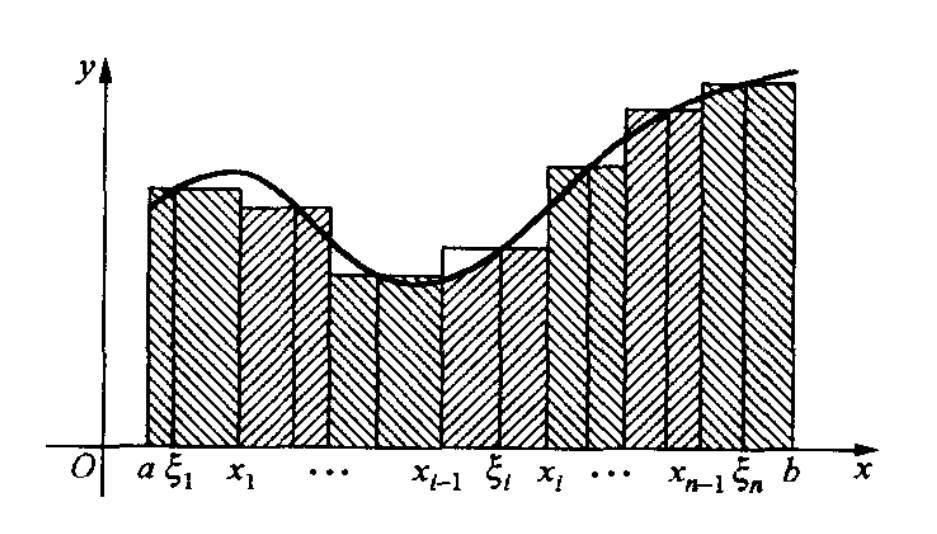
\includegraphics[width=\textwidth]{5.1.png} % 无需重复指定宽度  
\end{myimagebox}     
\caption{\label{fig:5.1}曲边梯形的面积}   
\end{figure}

对于一个定义在区间$[a,b]$的连续函数$f(x)$,计算图5.1的曲边面积该如何?我们在$[a,b]$插入一系列的点$x_0,x_1...x_n$使得:$a=x_0<x_1<x_2<..<x_{n-1}<x_n=b$。那么在每个小区间$[x_{i-1},x_i]$上,函数的凸性与直线$x=x_{i-1},x=x_{i}$都形成了小曲边梯形$S_i$,面积的近似值为:
\begin{align*}
    S_i\approx (x_{i}-x_{i-1})f(\xi_i)
\end{align*}

其中$\xi_i$是区间内的任意一点。而从直观上说,当分点越密集的时候,这个近似越准确,因此曲边梯形面积可以表示为:
\begin{align*}
    S=\lim_{\lambda\to 0}\sum_{i=1}^n f(\xi_i)\Delta x_i
\end{align*}

其中\textbf{$\lambda$是最长子区间的长度,因为我们并未要求点集把区间$[a,b]$等分},因此最长子区间长度如果趋近于0,就相当于我们的分割是无限密集的。

而\textbf{为什么$\xi$是任取的}?一个是子区间的长度趋近于0,因此取极限并不影响结果。其次如果$\xi$都去取函数在区间的最大值和最小值的点,求和后得到\textbf{达布大和与达布小和,求极限后二者的值是相等}的(可以证明),根据夹逼定理定积分的值唯一。

因此我们引出定积分的定义(接下来我们说的定积分都是Riemann黎曼积分):
\begin{tcolorbox}[
    colback=bac2,     % 极浅黄色背景
    colframe=fra2,   % 浅黄色边框
    coltitle=white,             % 标题文字白色
    coltext=tex2,
    title=Riemann定积分的定义,
    fonttitle=\bfseries,        % 标题加粗
arc=3mm,                     % 圆角稍大
breakable
]
设函数$f(x)$在区间$[a,b]$有定义:
\begin{enumerate}
    \item 称点集$P=\{x_0,x_1,...x_{n-1},x_n\}$是$[a,b]$上的一个\textbf{分划},如果满足条件$a=x_0<x_1<...<x_{n-1}<x_n=b$。

    记$\Delta x_i=x_i-x_{i-1},i=1\sim n$,并称$\lambda=\max\{\Delta x_i\}$为分划$P$的细度。如果$\Delta x_i\equiv \frac{b-a}{n}$,称$P$为等距分划。

    \item 设$P$为区间$[a.b]$一个分划,对每个子区间$[x_{i-1},x_i]$\textbf{任取}$\xi_i\in[x_{i-1},x_i]$,则称$\xi=\{\xi_1,\xi_2...\xi_n\}$是一个介点集。 称和式$\sum_{i=1}^n f(\xi_i)\Delta x_i$是函数$f(x)$在区间$[a,b]$的\textbf{黎曼和}。

    \item 设$I$是一个实数,并且有:
    \begin{align}
        \lim_{\lambda\to 0}\sum_{i=1}^n f(\xi_i)\Delta x_i=I
    \end{align}

    则称函数$f(x)$在区间$[a,b]$上\textbf{黎曼可积},记作$f\in R[a,b]$,定积分$I$写作:
    \begin{align*}
        \int _a^b f(x)=I
    \end{align*}
\end{enumerate}
\end{tcolorbox}

所以根据定积分的定义,定积分需要进行四步:\textbf{分割——找介值——计算黎曼和——取极限}。我们要注意,\textbf{分割和找介值的步骤都是任意的},只要最后能满足$\lambda\to 0$即可。如果不同分割和找介值计算的结果不同,说明这个函数\textbf{不可积}。我们接下来看一个例子:

\begin{tcolorbox}[
    colback=bac1,     % 极浅黄色背景
    colframe=fra1,   % 浅黄色边框
    coltitle=white,             % 标题文字白色
    coltext=tex1,
    title=用到的求和公式,
    fonttitle=\bfseries,        % 标题加粗
arc=3mm,                     % 圆角稍大
breakable
]
平方和公式和立方和公式可以写作:
\begin{align*}
    &1^2+2^2+...+n^2=\frac{n(n+1)(2n+1)}{6}\\
    &1^3+2^3+...+n^3=\frac{n^2(n+1)^2}{4}\tag{5-1}
\end{align*}
\end{tcolorbox}
\textbf{例}:利用定积分的定义证明。
\begin{align*}
    \int_0^1 x\mathrm{d}x=\frac{1}{2}
\end{align*}

\textbf{解}:我们第一种办法是\textbf{等分区间},介点取\textbf{区间的右端点}。记$x_k=\frac{k}{n}$,其中$k=0\sim n$。我们计算每一小块的面积:
\begin{align*}
    S_i=\Delta x_i\cdot f(x_i)=\frac{1}{n}\cdot \frac{i}{n}=\frac{i}{n^2}
\end{align*}

因此黎曼和可以写作:
\begin{align*}
    S_n=\sum_{i=1}^nS_i=\frac{1}{n^2}\sum_{i=1}^n i=\frac{1+n}{2n}
\end{align*}

这里$\lambda=\frac{1}{n}$,当去取极限的时候,$\lambda\to 0,n\to \infty$,因此$I=\frac{1}{2}$,计算完毕。

第二种办法是\textbf{不等分区间},介点取\textbf{区间的右端点}。记$x_k=\frac{k^2}{n^2}$,其中$k=0\sim n$。我们计算每一小块的面积:
\begin{align*}
    S_i=\Delta{x_i}\cdot f(x_{i})=(\frac{i^2}{n^2}-\frac{(i-1)^2}{n^2})\cdot\frac{i^2}{n^2}=\frac{2i^3-i^2}{n^2}
\end{align*}

因此黎曼和可以写作:
\begin{align*}
    S_n=\sum_{i=1}^nS_i=\frac{1}{n^2}\sum_{i=1}^n (2i^3-i^2)=\frac{(n+1)^2}{2n^2}-\frac{(n+1)(2n+1)}{6n^3}\to\frac{1}{2}
\end{align*}

在定积分中,我们要求积分上限大于积分下限。若上下限相等,定积分为0,若上限大于下限,则等于上下限互换后积分的相反数。

接下来我们将讨论定积分的可积性,在书上未对定积分可积性的判断做过多解释,我们这里做简短补充。首先我们说明:\textbf{函数黎曼可积一定在闭区间上有界}。它不要求函数在区间上的连续性,分段函数有界也可积。我们将对这个命题进行证明。

记$\int_a^b f(x)\mathrm{d}x=I$,从定积分定义,对于$\varepsilon=1$,存在一个分划$P$,使得对于这个分划下的任意介点集$\xi$都成立:
\begin{align*}
   | \sum_{i=1}^n f(\xi_i)\Delta x_i-I|<1
\end{align*}

我们接下来证明函数在每个$I_i=[x_{i-1},x_i]$上有界。对于一个确定的子区间$I_i$,固定其他的$\xi_k (i\neq k)$,则有:
\begin{align*}
    \frac{1}{\Delta x_i}(I-1-\sum_{k\neq i}f(\xi_k)\Delta x_k)<f(\xi_i)< \frac{1}{\Delta x_i}(I+1-\sum_{k\neq i}f(\xi_k)\Delta x_k)
\end{align*}

由于$\xi_i$是区间$I_i$的任意值,因此函数有界证毕。

接下来我们补充对可积函数的充要条件介绍。我们先引入这样的概念:函数在$[a,b]$上有界并且$P$是一个分划,对$i=1\sim n$,分别记$M_i,m_i$为区间$[x_{i-1},x_i]$上的最大值和最小值,称$w_i=M_i-m_i$时函数在$[x_{i-1},x_i]$的振幅。

\begin{tcolorbox}[
    colback=bac1,     % 极浅黄色背景
    colframe=fra1,   % 浅黄色边框
    coltitle=white,             % 标题文字白色
    coltext=tex1,
    title=可积的充要条件,
    fonttitle=\bfseries,        % 标题加粗
arc=3mm,                     % 圆角稍大
breakable
]
\textbf{可积第一充要条件}:有界函数可积的充分必要条件为:
\begin{align*}
    \lim_{\lambda\to 0}\sum_{i=1}^n w_i\Delta x_i=0\tag{5-2}
\end{align*}

\textbf{可积第二充要条件}:有界函数可积的充要条件为$\forall \varepsilon>0,\exists P$分划,使得:
\begin{align*}
    \sum w_i\Delta x_i<\varepsilon\tag{5-3}
\end{align*}
\end{tcolorbox}

我们这里不对这两个定理进行过多的证明,而是给出Riemann可积函数的三个结论:
\begin{tcolorbox}[
    colback=bac2,     % 极浅黄色背景
    colframe=fra2,   % 浅黄色边框
    coltitle=white,             % 标题文字白色
    coltext=tex2,
    title=黎曼可积函数的性质,
    fonttitle=\bfseries,        % 标题加粗
arc=3mm,                     % 圆角稍大
breakable
]
\begin{enumerate}
    \item 设$f\in C[a,b]$,则$f\in R[a,b]$。
    \item 设$f$在$[a,b]$有界且只有有限个间断点,则$f\in R[a,b]$。 
    \item 设$f$在$[a,b]$单调,则$f\in R[a,b]$。
\end{enumerate}
\end{tcolorbox}

\subsubsection{定积分的性质}
有关极限的定理在定积分中同样适用。
\begin{tcolorbox}[
    colback=bac2,     % 极浅黄色背景
    colframe=fra2,   % 浅黄色边框
    coltitle=white,             % 标题文字白色
    coltext=tex2,
    title=定积分的性质,
    fonttitle=\bfseries,        % 标题加粗
arc=3mm,                     % 圆角稍大
breakable
]
\begin{enumerate}
    \item 设$f\in R[a,b],f\geq 0$,则:
    \begin{align*}
        \int_a^b f(x)\mathrm{d}x\geq 0
    \end{align*}
    \item 设$f\in R[a,b],g\in R[a,b]$,则$f\pm g\in R[a,b]$,且:
    \begin{align*}
        \int_a^b f(x)\mathrm{d}x\pm\int_a^b g(x)\mathrm{d}x=\int_a^b f(x)\pm g(x)\mathrm{d}x
    \end{align*}
    \item 设$f\in R[a,b],g\in R[a,b]$,$f(x)\geq g(x)$,则:
    \begin{align*}
        \int_a^b f(x)\mathrm{d}x\geq \int_a^b g(x)\mathrm{d}x
    \end{align*}
 \item 设$f\in R[a,b]$,则$\forall c\in[a,b]$,都有$f\in R[a,c],R[c,b]$,且:
 \begin{align*}
     \int_a^b f(x)\mathrm{d}x=\int_a^cf(x)\mathrm{d}x+\int_c^b f(x)\mathrm{d}x
 \end{align*}
 \item 设$f\in R[a,b],g\in R[a,b]$,$f,g$在区间上只有有限个点不相同,则:
 \begin{align*}
     \int_a^b f(x)\mathrm{d}x=\int_a^b g(x)\mathrm{d}x
 \end{align*}

 \item  设$f\in R[a,b]$,则$|f|\in R[a,b]$,且有:
 \begin{align*}
     |\int_a^b f(x)\mathrm{d}x|\leq \int_a^b |f(x)|\mathrm{d}x\tag{5-4}
\end{align*}
\end{enumerate}
\end{tcolorbox}

3-4的结论是非常重要的,其证明思路可以这样理解:左侧是所有曲边梯形面积和的绝对值,但是左侧每一块分面积有正有负。而右侧是所有曲边梯形分面积的绝对值之和。

接下来我们介绍积分中值定理。\textbf{积分第一中值定理的特殊情况是必须要掌握}的,对于积分第一中值定理和对其的延伸读者可自行学习。
\begin{tcolorbox}[
    colback=bac1,     % 极浅黄色背景
    colframe=fra1,   % 浅黄色边框
    coltitle=white,             % 标题文字白色
    coltext=tex1,
    title=积分第一中值定理,
    fonttitle=\bfseries,        % 标题加粗
arc=3mm,                     % 圆角稍大
breakable
]
设$f,g\in R[a,b],m\leq f(x)\leq M,\forall x\in[a,b]$,且\textbf{$g$在$[a,b]$上不变号}。则$\exists \eta\in [m.M]$,使得:
\begin{align*}
    \int_a^b f(x)g(x)\mathrm{d}x=\eta \int_a^b g(x)\mathrm{d}x\tag{5-5}
\end{align*}

特别地,当$f\in C[a,b]$时,存在$\xi\in[a,b]$,使得:
\begin{align*}
    \int_a^b f(x)\mathrm{d}x=f(\xi)(b-a)\tag{5-6}
\end{align*}
\end{tcolorbox}

我们先对5-6进行证明,这是需要读者掌握的:由于函数连续,因此在区间上存在最大值和最小值
$m,M$,使得$m\leq f(x)\leq M$,然后在区间$[a,b]$上积分:
\begin{align*}
  \int_a^b m\mathrm{d}x \leq  \int_a^b f(x)\mathrm{d}x\leq \int_a^b M\mathrm{d}x
\end{align*}

因此得到:
\begin{align*}
    m\leq\frac{\int_a^b f(x)\mathrm{d}x}{b-a}\leq M
\end{align*}

根据连续函数介值定理,中间的数字肯定能在$x=c$处取到,也就是说$f(c)$可以表示不等式中间的值,证毕。

而对于积分第一中值定理,我们不妨令$g(x)\geq 0$,则:
\begin{align*}
    \int_a^b mg(x)\mathrm{d}x\leq \int_a^b f(x)g(x)\mathrm{d}x\leq \int _a^b Mg(x)\mathrm{d}x
\end{align*}

函数不连续并不影响到函数在闭区间上存在最大值和最小值(最值定理不影响),只会影响介值定理的正确性。因此我们得知肯定$\exists \eta\in[m.M]$使得$\eta\int g=\int fg$,证毕。

\begin{tcolorbox}[
    colback=bac1,     % 极浅黄色背景
    colframe=fra1,   % 浅黄色边框
    coltitle=white,             % 标题文字白色
    coltext=tex1,
    title=积分第一中值定理拓展,
    fonttitle=\bfseries,        % 标题加粗
arc=3mm,                     % 圆角稍大
breakable
]

若$f\in C[a,b],g\in R[a,b]$且不编号,则$\exists\eta\in[m.N]=f([a,b])$,使得:
\begin{align*}
    \int_a^b f(x)g(x)\mathrm{d}x=f(\xi)\int_a^b g(x)\mathrm{d}x\tag{5-7}
\end{align*}

其中$\eta=f(\xi),\xi\in[a,b]$
\end{tcolorbox}

这是因为$f(x)$连续后保证了介值定理的成立,因此在第一中值定理中的$\eta$是可以在函数$f(x)$找到一点的。

\subsubsection{变限积分与微积分基本定理}
我们先介绍变上限积分:假设函数$f(x)$在区间$[a,b]$连续,则对于它我们可以定义一个变上限积分:
\begin{align*}
    F_0(x)=\int_a^x f(t)\mathrm{d}t
\end{align*}

这个积分的参数就是积分上限$x$。因此变上限积分是关于积分上限的函数。我们说明:在这种情况下\textbf{变上限积分可导,并且$F'_0(x)=f(x)$}。也就是说变上限积分的变化率就是积分终点的函数值。从几何上这是很简单的,因为积分面积的变化率就是尾端面积微元的值。当然这也给出来原函数存在的一个充分条件,回答了上一章我们讨论原函数存在性的问题。如果是变下限积分,我们添加一个负号就可以使之变成变上限积分。我们不再赘述定理的证明(书上已经给出),而是给出变限积分的求导公式:
\begin{tcolorbox}[
    colback=bac1,     % 极浅黄色背景
    colframe=fra1,   % 浅黄色边框
    coltitle=white,             % 标题文字白色
    coltext=tex1,
    title=变限积分的求导公式,
    fonttitle=\bfseries,        % 标题加粗
arc=3mm,                     % 圆角稍大
breakable
]
对于变限积分$F(x)=\int_{\sigma(x)}^{\varphi(x)}f(t)\mathrm{d}t$,其关于$x$的导数为:
\begin{align*}
    F'(x)=f[\varphi(x)]\varphi'(x)-f[\sigma(x)]\sigma'(x)\tag{5-8}
\end{align*}
\end{tcolorbox}

\textbf{例:}(1)计算变限积分的导数$F(x)=\int_{x^2}^x\sqrt{1+t}\mathrm{d}t$。

(2)求下面函数的二阶导数:
\begin{align*}
    G(x)=\int_0^x\left(e^t\int_0^t \sqrt{\sin z}\mathrm{d}z\right)\mathrm{d}t
\end{align*}

(3)设函数$f\in C[0,+\infty),a>0$,证明下式成立:
\begin{align*}
    \int_0^a\left(\int_0^x f(t)\mathrm{d}t\right)\mathrm{d}x=\int_0^a f(x)(a-x)\mathrm{d}x
\end{align*}

\textbf{解:}(1)直接套用公式计算:
\begin{align*}
    F'(x)=\sqrt{1+x}-2x\sqrt{1+x^2}
\end{align*}

(2)套用两次公式即可:
\begin{align*}
    G'(x)&=e^x\int_0^x\sqrt{\sin z}\mathrm{d}z \\
    G''(x)&=e^x\int_0^x\sqrt{\sin z}\mathrm{d}z+e^x\sqrt{\sin x}
\end{align*}

(3)把$a$看做非负变量,左右两边对$a$求导,得到:
\begin{align*}
   \left( \int_0^a\left(\int_0^x f(t)\mathrm{d}t\right)\mathrm{d}x\right)'=\left(\int_0^a f(x)(a-x)\mathrm{d}x\right)'=\int_0^a f(x)\mathrm{d}x
\end{align*}

接下来我们介绍微积分基本定理。它是连接不定积分和定积分的桥梁,把计算定积分的问题转化成了计算不定积分的问题。其内容如下:
\begin{tcolorbox}[
    colback=bac1,     % 极浅黄色背景
    colframe=fra1,   % 浅黄色边框
    coltitle=white,             % 标题文字白色
    coltext=tex1,
    title=微积分基本定理,
    fonttitle=\bfseries,        % 标题加粗
arc=3mm,                     % 圆角稍大
breakable
]
设函数$f(x)$在\textbf{闭区间$[a,b]$连续},$F(x)$是$f(x)$在开区间$(a,b)$一个原函数,并且$F(x)$在\textbf{闭区间$[a,b]$连续},则我们有\textbf{牛顿——莱布尼茨公式}:
\begin{align*}
    \int_a^b f(x)\mathrm{d}x=F(b)-F(a)\tag{5-9}
\end{align*}
\end{tcolorbox}

我们令$F_0(x)=\int_a^x f(t)\mathrm{d}t$,那么$F'_0(x)=f(x)$,这样$F'(x)-F'(x_0)=0$,于是$F(x)=F_0(x)+C$。而由连续性,$F(a)=\lim_{x\to a+0}F_0(x)+C=F_0(a)+c=C$,同理得到$F(b)=F_0(b)+C$,相减即可。

\textbf{例}:求下面两个定积分的值。
\begin{align*}
    (1) \int_0^1 (e^x+x)\mathrm{d}x\qquad (2)\int_{-1}^2f(x)\mathrm{d}x\qquad f(x)=\begin{cases}
        x & -1\leq x<0\\
        0 & 0\leq x<1\\
        x & 1\leq x\leq 2
    \end{cases}
\end{align*}

\textbf{解}:(1)直接转化为计算不定积分的值:
\begin{align*}
    \int_0^1 e^x+x\mathrm{d}x=\left. e^x+\frac{1}{2}x^2\right|_0^1=e-\frac{1}{2}
\end{align*}

(2)我们把分段函数的定积分拆成一段一段:
\begin{align*}
    \int_{-1}^2 f(x)\mathrm{d}x=\int_{-1}^ 0 x\mathrm{d}x+\int_1^2 x\mathrm{d}x=1
\end{align*}

利用牛顿——莱布尼茨公式,我们也可以计算黎曼和。如下面的这道例题:

\textbf{例:}计算黎曼和$\lim_{n\to\infty}\sum_{k=1}^n (\frac{k}{n}+1)^3\frac{1}{n}$。

\textbf{解:}我们需要观察这个黎曼和,找到其是对哪个函数,哪个区间的分割。显然$\frac{1}{n}$是区间长度,一共有$n$个区间,因此积分长度为1.另一方面$(\frac{k}{n}+1)^3$是区间上一点的取值。可以得到其是在$[0,1]$区间上进行积分,积分函数为$(1+x)^3$,因此原式即为$\int_0^1 (1+x^3)\mathrm{d}x=\frac{15}{4}$。

我们最后看一个例子,这个例子非常容易犯错。设$f\in R[A,B]$,并且$a,b\in(A,B)$是函数的两个连续点。证明:
\begin{align*}
    \lim_{h\to 0}\int_a^b\frac{f(x+h)-f(x)}{h}\mathrm{d}x=f(b)-f(a)
\end{align*}

\begin{tcolorbox}[
    colback=bac2,     % 极浅黄色背景
    colframe=fra2,   % 浅黄色边框
    coltitle=white,             % 标题文字白色
    coltext=tex2,
    title=错误证法,
    fonttitle=\bfseries,        % 标题加粗
arc=3mm,                     % 圆角稍大
breakable
]
一个非常经典的错误如下:
\begin{align*}
    \lim_{h\to 0}\int_a^b\frac{f(x+h)-f(x)}{h}\mathrm{d}x&=\int_a^b\lim_{h\to 0}\frac{f(x+h)-f(x)}{h}\mathrm{d}x\\
    &=\int_a^b f'(x)\mathrm{d}x=f(b)-f(a)
\end{align*}

但是这每一步都是错误的,这是因为:
\begin{enumerate}
    \item 第一步定积分和极限是不能任意交换顺序的。
    \item 第二步并没有说函数$f(x)$在整个开区间上可导。
    \item 第三步也没有说导函数一定是可以积分。
\end{enumerate}
\end{tcolorbox}

这道题正确的做法如下,核心是利用变量代换改变积分限。
\begin{align*}
     \lim_{h\to 0}\int_a^b\frac{f(x+h)-f(x)}{h}\mathrm{d}x&=\lim_{h\to 0}\frac{1}{h}\left(\int_a^b f(x+h)\mathrm{d}x-\int_a^b f(x)\mathrm{d}x\right)\\
     &=\lim_{h\to 0}\frac{1}{h}\left(\int_{a+h}^{b+h} f(x)\mathrm{d}x-\int_a^b f(x)\mathrm{d}x\right)\\
     &=\lim_{h\to 0}\frac{1}{h}\left(\int_b^{b+h} f(x)\mathrm{d}x-\int_a^{a+h} f(x)\mathrm{d}x\right)\\
     &=f(b)-f(a)
\end{align*}

\subsection{定积分的计算}
\subsubsection{定积分的换元积分法和分部积分法}
根据微积分基本定理,定积分计算可以转化成不定积分的计算。因此定积分的还原积分法和分部积分法与不定积分类似。
\begin{tcolorbox}[
    colback=bac2,     % 极浅黄色背景
    colframe=fra2,   % 浅黄色边框
    coltitle=white,             % 标题文字白色
    coltext=tex2,
    title=定积分的换元积分法和分部积分法:,
    fonttitle=\bfseries,        % 标题加粗
arc=3mm,                     % 圆角稍大
breakable
]
\textbf{换元积分法}:设函数$f(x)$在区间$[a,b]$上连续,又设函数$\varphi(t)$在区间$[\alpha,\beta]$上的\textbf{导数连续},且当$t$在$[\alpha,\beta]$变动时$\varphi(t)$在$[A,B]$中变动,假定$a,b\in[A,B],\varphi (\alpha)=a,\varphi(\beta)=b$,那么:
\begin{align*}
    \int_a^b f(x)\mathrm{d}x=\int_\alpha^\beta f(\varphi(t))\varphi'(t)\mathrm{d}t
\end{align*}

\textbf{分部积分法}:设函数$u(x),v(x)$在区间$[a,b]$可导并且导数在$[a,b]$连续,我们有:
\begin{align*}
    \int_a^b u(x)v'(x)\mathrm{d}x=u(x)v(x)|_a^b-\int_a^b v(x)u'(x)\mathrm{d}x
\end{align*}
\end{tcolorbox}

我们接下来看一个例子,这个例子在日后计算多重积分有广泛的运用:

\textbf{例}:假设$n$是正整数且$n\geq 2$,计算下面的两个积分:
\begin{align*}
    I_n=\int_0^\frac{\pi}{2} \sin^n x\mathrm{d}x\qquad I_n=\int_0^\frac{\pi }{2}\cos^n x\mathrm{d}x
\end{align*}

\textbf{解}:我们先说明这两个积分是相等的。对于第二个积分我们采用换元积分法,令$t=\frac{\pi}{2}-x$,此时积分上下限变为了$\frac{\pi}{2},0$。因此:
\begin{align*}
    I_n=\int_0^\frac{\pi }{2}\cos^n x\mathrm{d}x=\int_{\pi/2}^0 \cos^n(\frac{\pi}{2}-t)\mathrm{d}(\frac{\pi}{2}-t)=\int_0^\frac{\pi}{2} \sin^n t\mathrm{d}t
\end{align*}

我们只计算第一个式子,采用分部积分法计算递推式:
\begin{align*}
    I_n&=-\int_0^{\frac{\pi}{2}}\sin^{n-1}x\mathrm{d}(\cos x)\\
&=\left.-(\sin^{n-1}x\cos x)\right|_0^{\frac{\pi}{2}}+\int_0^{\frac{\pi}{2}}\cos x\mathrm{d}(\sin^{n-1}x)\\
&=(n-1) \int_0^{\frac{\pi}{2}}\sin^{n-1}x\cos^2 x\mathrm{d}x\\
&=(n-1) \int_0^{\frac{\pi}{2}}\sin^{n-1}x(1-\sin^2x)\mathrm{d}x\\
&=(n-1)I_{n-2}-(n-1)I_n=\frac{n-1}{n}I_{n-2}
\end{align*}

接下来计算初值条件:
\begin{align*}
    I_0=\frac{\pi}{2}\qquad I_1=1
\end{align*}
\begin{tcolorbox}[
    colback=bac1,     % 极浅黄色背景
    colframe=fra1,   % 浅黄色边框
    coltitle=white,             % 标题文字白色
    coltext=tex1,
    title=Wallis公式与Wallis极限,
    fonttitle=\bfseries,        % 标题加粗
arc=3mm,                     % 圆角稍大
breakable
]
上述积分的结果被写作Wallis公式,即:
\begin{align*}
    &\int_0^\frac{\pi}{2}\sin^{2k}x\mathrm{d}x=\int_0^\frac{\pi}{2}\cos^{2k} x\mathrm{d}x
=\frac{(2k-1)!!}{(2k)!!}\cdot\frac{\pi}{2}\\
&\int_0^\frac{\pi}{2}\sin^{2k+1}x\mathrm{d}x=\int_0^\frac{\pi}{2}\cos^{2k+1} x\mathrm{d}x
=\frac{(2k)!!}{(2k+1)!!}\tag{5-10}
\end{align*}

例如$I_6=\frac{5\cdot 3\cdot 1}{6\cdot 4\cdot 2}\cdot\frac{\pi}{2}=\frac{5\pi}{32}$。同时我们也可以根据这个公式推导Wallis极限:
\begin{align*}
    \lim_{n\to\infty}\left[\frac{(2n)!!}{(2n-1)!!}\right]^2\frac{1}{2n+1}=\frac{\pi}{2}\tag{5-11}
\end{align*}

由于$\sin^{2k+1}x<\sin^{2k}x<\sin^{2k-1}x$,因此积分之后$I_{2k+1}<I_{2k}<I_{2k-1}$,代入Wallis积分:
\begin{align*}
   &\frac{(2k)!!}{(2k+1)!!}<\frac{(2k-1)!!}{(2k)!!}\frac{\pi}{2}<\frac{(2k-2)!!}{(2k-1)!!}\\
&1<\frac{(2k-1)!!(2k+1)!!}{(2k)!!(2k)!!}\frac{\pi}{2}<\frac{2k+1}{2k}  
\end{align*}

当$k\to\infty$时,利用夹逼定理,中间的极限为1,化简得到所求极限。
\end{tcolorbox}

在定积分中计算时,一定要注意换元积分法的适用范围,函数$\varphi(t)$在区间$[\alpha,\beta]$上的\textbf{导数连续},换言之积分后的\textbf{原函数要连续}。例如计算下面的定积分:
\begin{align*}
    \int_0^\pi\frac{\mathrm{d}x}{2+\cos x}=\left.\frac{1}{\sqrt{3}}\arctan(\frac{\tan x}{\sqrt{3}})+C\right|_0^\pi
\end{align*}

这个做法是错误的,因为没考虑到原函数在定义域上有间断点$x=\frac{\pi}{2}$。

\textbf{例:}计算下面的定积分。
\begin{align*}
    (1)\int_0^a x^4\sqrt{a^2-x^2}\mathrm{d}x\;(a>0)\qquad (2)\int_{-\pi/2}^{\pi/2}\frac{\sin ^2x}{1+e^x}\mathrm{d}x\qquad  (3)\int_0^{\pi/2}\sin x\ln\sin x\mathrm{d}x
\end{align*}

\textbf{解:}(1)进行三角换元$x=a\cos t$,注意上下限的对应:
\begin{align*}
\int_0^a x^4\sqrt{a^2-x^2}\mathrm{d}x&=\int_\frac{\pi}{2}^0a^4\cos^4t\cdot a\sin t\cdot (-a\sin t)\mathrm{d}t\\
&=\int_0^\frac{\pi}{2}a^6\cos^4t\mathrm{d}t- \int_0^\frac{\pi}{2}a^6\cos^6t\mathrm{d}t  \\
&=\frac{\pi}{32}a^6  
\end{align*}

(2)这个积分在不定积分范围内是很难做的,但是通过变量代换,我们可以化简定积分。
\begin{align*}
\int_{-\pi/2}^{\pi/2}\frac{\sin ^2x}{1+e^x}\mathrm{d}x&=\int_{0}^{\pi/2}\frac{\sin ^2x}{1+e^x}\mathrm{d}x+\int_{-\pi/2}^{0}\frac{\sin ^2x}{1+e^x}\mathrm{d}x\\
&=\int_{0}^{\pi/2}\frac{\sin ^2x}{1+e^x}\mathrm{d}x-\int_{\pi/2}^0\frac{\sin^2 t}{1+e^{-t}}(-\mathrm{d}t) \\
&=\int_{0}^{\pi/2}\frac{\sin ^2x}{1+e^x}\mathrm{d}x+\int_0^{\pi/2}\frac{\sin^2 x}{1+e^{-x}}\mathrm{d}x\\
&=\int_0^{\pi/2}\sin^2x\mathrm{d}x=\frac{\pi}{4}   
\end{align*}

(3)如果直接用$\cos x$分部积分,则:
\begin{align*}
    I&=\int_0^\frac{\pi}{2}\ln\sin x\mathrm{d}(-\cos x)\\
    &=-\cos \ln\sin x|_0^\frac{\pi}{2}+\int_0^\frac{\pi}{2}\cos x\mathrm{d}
    ln\sin x
\end{align*}

但这个式子右边的第一项是无穷大的,因此离我们需要进行一些修改:
\begin{align*}
    I&=\int_0^\frac{\pi}{2}\ln\sin x\mathrm{d}(1-\cos x)\\
        &=(1-\cos x)\ln\sin x|_0^\frac{\pi}{2}-\int_0^\frac{\pi}{2}(1-\cos x)\mathrm{d}\ln\sin x\\
     &=-\int_0^\frac{\pi}{2}\frac{\sin x\cos x}{1+\cos x}\mathrm{d}x\\
     &=\int_0^\frac{\pi}{2}(-\sin x+\frac{\sin x}{1+\cos x})\mathrm{d}x\\
    &=[\cos x-\ln(1+\cos x)]|_0^\frac{\pi}{2}=\ln 2-1
\end{align*}

\subsubsection{定积分的对称性和递推关系}
和不定积分不同的是,定积分存在积分限,因此有时虽然我们不能求出原函数,但是通过变换积分限和积分函数,利用它们的性质可以解特定的定积分。在上一章中我们其实已经给出了一些特殊的例子(如上一题第二个积分,Wallis积分),它们蕴含着对称性、变量替换、递推等思想。接下来我们依次进行讲解。

我们先来看对称性。我们考虑一个关于原点对称的积分区间$[-a,a]$。如果被积函数是偶函数,那么其积分就相当于在$[0,a]$上积分值的2倍。如果被积函数是奇函数,那么积分值就为0。另一方面,我们考虑一个周期为$T$的周期函数,那么在$[0,a]$上的积分就可以等于$[nT,a+nT]$上的积分。这些道理都是显然意见的。

那么同样的,在高中我们学过各种各样的对称。例如关于$x=a$轴对称,关于$(a,0)$中心对称等。这些对称性也可以辅助定积分的计算。

\textbf{例:}利用对称性计算下面的定积分。
\begin{align*}
    (1)\int_0^8 (x-[x])\mathrm{d}x\quad (2)\int_0^\pi \frac{x\sin x}{1+\cos^2 x}\mathrm{d}x\quad (3)\int_0^1\frac{\ln(1+x)}{1+x^2}\mathrm{d}x
\end{align*}

\textbf{解:}(1)这个函数的周期$T=1$,因此:
\begin{align*}
    I=8\int_0^1 (x-[x])\mathrm{d}x=8\int_0^1x\mathrm{d}x=4
\end{align*}

(2)不妨令$t=\pi-x$,因此原积分可以写作:
\begin{align*}
    I&=\int_0^\pi \frac{(\pi-t)\sin(\pi-t)}{1+\cos^2(\pi-t)}\mathrm{d}t\\
    &=\int_0^\pi \frac{(\pi-t)\sin t}{1+\cos^2 t}\mathrm{d}t
\end{align*}

我们将其与原来的形式相加,则发现分母就只剩下了$\pi \sin x$:
\begin{align*}
    I&=\frac{1}{2}\int_0^\pi \frac{\pi\sin x}{1+\cos^2 x}\mathrm{d}x\\
    &=\int_0^\frac{\pi}{2} \frac{\pi\sin x}{1+\cos^2 x}\mathrm{d}x\\
    &=-\pi\arctan(\cos x)|_0^{\pi/2}=\frac{\pi^2}{4}
\end{align*}

(3)我们继续做代换$x=\tan t,\mathrm{d}x=\sec^2 t\mathrm{d}t$,因此原式可以写作:
\begin{align*}
    I&=\int_0^\frac{\pi}{4}\ln(1+\tan t)\mathrm{d}t
\end{align*}

记$p=\frac{\pi}{4}-t$,则积分可以改写为:
\begin{align*}
    I&=\int_0^\frac{\pi}{4}\ln(1+\tan(\frac{\pi}{4}-t)\mathrm{d}t
\end{align*}

因此两式相加,得到:
\begin{align*}
    I&=\frac{1}{2}\int_0^\frac{\pi}{4}\ln(1+\tan t)+\ln(1+\frac{1-\tan t}{1+\tan t})\mathrm{d}t\\
    &=\frac{1}{2}\int_0^\frac{\pi}{4}\ln 2\mathrm{d}t\\
    &=\frac{\pi}{8}\ln 2
\end{align*}

利用递推公式计算定积分也是比较重要的。Wallis积分就展现了这一思路,本质上是利用分部积分法寻找递推关系。我们这里只补充一个例子:计算下面双参数定积分,其中$m,n$都是大于1的正整数。
\begin{align*}
    B(m,n)=\int_0^1 x^{m-1}(1-x)^{n-1}\mathrm{d}x
\end{align*}

\textbf{解}:利用分部积分法,令$x^{m-1}\mathrm{d}x=\mathrm{d}v,(1-x)^{n-1}=u$,则:
\begin{align*}
B(m,n)&=\left.\frac{x^m(1-x)^{n-1}}{m}\right|_0^1+\frac{n-1}{m}\int_0^1x^m(1-x)^{n-2}\mathrm{d}x\\
&=  \frac{n-1}{m}B(m+1,n-1)\\
&=\frac{(n-1)(n-2)...1}{m(m+1)...(m+n-2)} \int_0^1x^{m+n-2}\mathrm{d}x\\
&=\frac{(n-1)!(m-1)!}{(m+n-1)!} 
\end{align*}

\subsection{定积分的应用}
\subsubsection{几何应用}
定积分在几何上有非常多的应用。设平面上有一条弧$AB$,其方程使用参数方程表示出来的:
\begin{align*}
    \begin{cases}
        x=x(t)\\
        y=y(t)
    \end{cases}\quad t\in[\alpha,\beta]
\end{align*}

我们假设$x'(t),y'(t)$都是连续的,因此我们把这种曲线称作光滑曲线。光滑曲线是一定可以计算弧长的。
\begin{figure}[H]    
\centering     
\renewcommand{\figurename}{图}     
\renewcommand{\thefigure}{5.2}    
\begin{myimagebox}[width=0.25\textwidth] % 直接传入图片尺寸参数      
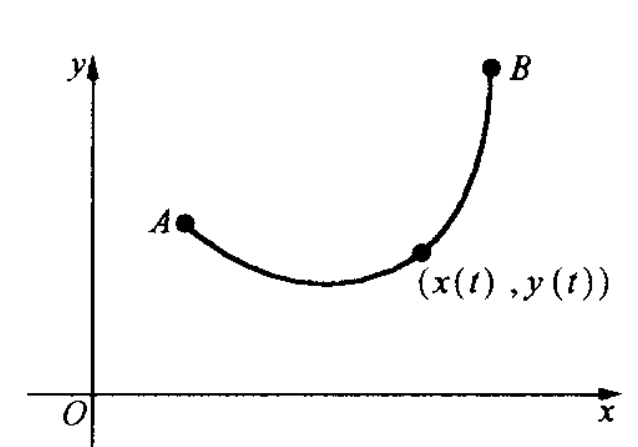
\includegraphics[width=\textwidth]{5.2.png} % 无需重复指定宽度  
\end{myimagebox}     
\caption{\label{fig:5.2}光滑曲线}   
\end{figure}

我们看图5.2光滑曲线,现在我们采用定积分的定义法去计算这条弧线的长度。我们把区间$[\alpha,\beta]$切成$n$登分,分点为$\alpha=t_0<t_1<...<t_n=\beta$。在曲线$AB$上也有对应的分点$M_i(x(t_i),y(t_i)),t=0\sim n$。记$\Delta s_i$是曲线$M_{i-1}M_{i}$的长度。当分点足够密集的时候,每一小段曲线弧都近似为一条直线段,因此:
\begin{align*}
    \Delta s_i\approx \sqrt{(x(t_i)-x(t_{i-1}))^2+(y(t_i)-y(t_{i-1}))^2}
\end{align*}

而当分点足够多时,$t_i$与$t_{i-1}$足够近,因此$\Delta x=x'(t_{i-1})\Delta t_i$。因此就有:
\begin{align*}
    \mathrm{d}s=\sqrt{x'(t)^2+y'(t)^2}\mathrm{d}t
\end{align*}

这被称作\textbf{弧微分}。求弧长只需要左右对$[\alpha,\beta]$积分即可。

如果弧的函数不是由参数方程给出而是由函数$y=f(x)$给出,我们可以代换$x=t,y=f(t)$。这也是参数方程。弧微分可以写作:
\begin{align*}
    \mathrm{d}s=\sqrt{1+f'(x)^2}\mathrm{d}x
\end{align*}

如果弧的函数是根据极坐标给出。极坐标的方程是$\rho=\rho(\theta)$,其中$x=\rho\cos\theta,y=\rho\sin \theta$。只需要把这个表达式直接带入到弧微分:
\begin{align*}
    \mathrm{d}s=\sqrt{\rho^2(\theta)+\rho'(\theta)^2}\mathrm{d}\theta
\end{align*}

\begin{tcolorbox}[
    colback=bac1,     % 极浅黄色背景
    colframe=fra1,   % 浅黄色边框
    coltitle=white,             % 标题文字白色
    coltext=tex1,
    title=弧微分的表示,
    fonttitle=\bfseries,        % 标题加粗
arc=3mm,                     % 圆角稍大
breakable
]
弧微分的三种表示方法为:
\begin{align*}
    &\mathrm{d}s=\sqrt{x'(t)^2+y'(t)^2}\mathrm{d}t\\
    &\mathrm{d}s=\sqrt{1+f'(x)^2}\mathrm{d}x\\
&\mathrm{d}s=\sqrt{\rho^2(\theta)+\rho'(\theta)^2}\mathrm{d}\theta\tag{5-12}
\end{align*}
\end{tcolorbox}

\textbf{例:}计算下述旋轮线的弧长。
\begin{align*}
    \begin{cases}
        x=R(\theta-\sin\theta)\\
        y=R(1-\cos\theta)
    \end{cases}\qquad \theta\in[0,2\pi]
\end{align*}

\textbf{解:}代入到我们的弧微分表达式:
\begin{align*}
    s&=\int_0^{2\pi}\sqrt{R^2(1-\cos\theta)^2+R^2\sin^2\theta}\mathrm{d}\theta\\
    &=R\int_0^{2\pi}\sqrt{2(1-\cos\theta)}\mathrm{d}\theta\\
    &=2R\int_0^{2\pi}|\sin\frac{\theta}{2}|\mathrm{d}\theta\\
    &=8R
\end{align*}

接下来我们用定积分计算旋转体的体积与侧面积。
\begin{figure}[H]    
\centering     
\renewcommand{\figurename}{图}     
\renewcommand{\thefigure}{5.3}    
\begin{myimagebox}[width=0.43\textwidth] % 直接传入图片尺寸参数      
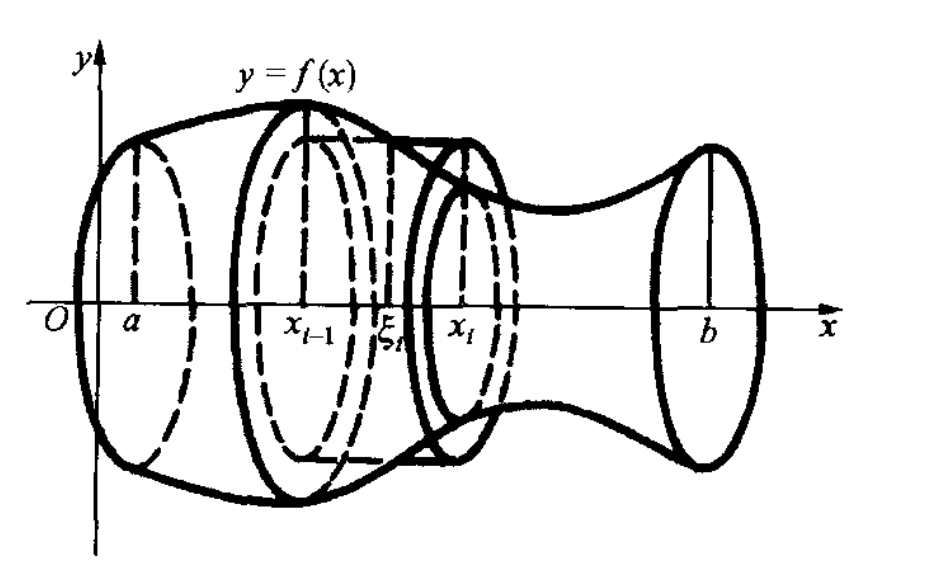
\includegraphics[width=\textwidth]{5.3.png} % 无需重复指定宽度  
\end{myimagebox}     
\caption{\label{fig:5.3}旋转体的体积与侧面积}   
\end{figure}

图5.3是一个旋转体,我们考虑$y=f(x)$一个非负函数,其绕$x$轴转一圈形成了旋转体。将区间用分点分开,在区间$[x_{i-1},x_i]$处,分点足够紧密的时候是一个圆柱体,其体积微元和侧面积微元即就是:
\begin{align*}
    \Delta V_i&=\Delta x_i\cdot \pi \cdot f^2(x)\\
    \Delta S_i&=\Delta s_i\cdot 2\pi\cdot f(x)
\end{align*}

其中$\Delta s_i$是弧微元。将等式两侧进行积分即可计算:
\begin{tcolorbox}[
    colback=bac2,     % 极浅黄色背景
    colframe=fra2,   % 浅黄色边框
    coltitle=white,             % 标题文字白色
    coltext=tex2,
    title=旋转体的侧面积和体积,
    fonttitle=\bfseries,        % 标题加粗
arc=3mm,                     % 圆角稍大
breakable
]
旋转体的体积可以写作:
\begin{align*}
    V=\pi\int_a^b f^2(x)\mathrm{d}x\tag{5-13}
\end{align*}

旋转体的侧面积可以写作:
\begin{align*}
    S=2\pi \int_a^b f(x)\sqrt{1+f'(x)^2}\mathrm{d}x\tag{5-14}
\end{align*}
\end{tcolorbox}

\subsubsection{其他应用(选学)}
这一部分仅作为拓展,读者可自行学习。我们在这里主要再介绍四个问题:\textbf{对积分求极限、利用积分中值定理求定积分、积分不等式、定积分与序列极限}。

设有一类函数$f_n(x)\in R[a,b]$,并且这一列函数在区间上都有$\lim_{n\to\infty}f_n(x)=f(x)$,那么积分符号和极限符号是否可以互换?也就是说是否成立:
\begin{align*}
    \lim_{b\to\infty}\int_a^b f_n(x)\mathrm{d}x=\int_a^b f(x)\mathrm{d}x
\end{align*}

事实上是\textbf{不一定成立的}。关于是否成立要在高数(II)中进行讲解。那么我们如何求一个定积分的极限?我们通常使用的方法就是\textbf{分区间估算}。下面一道题就是典型的计算定积分极限的例题。

\textbf{例}:证明下述极限成立。
\begin{align*}
\lim_{n\to\infty}\int_0^{\pi/2}\sin^n x\mathrm{d}x=0
\end{align*}

\textbf{解}:首先我们要考虑,对于这个积分,在接近$\frac{\pi}{2}$时被积函数都会迅速到1,而其余部分的值一般比较小。因此我们采用分而治之的办法:我们把积分区间分成$[0,\frac{\pi-\varepsilon}{2}],[\frac{\pi-\varepsilon}{2},\frac{\pi}{2}]$两个部分,积分分别为$I_1,I_2$,并且对被积函数进行放大:
\begin{align*}
    I_1+I_2\leq \frac{\pi-\varepsilon}{2}\cdot \sin^n \frac{\pi-\varepsilon}{2}+\frac{\varepsilon}{2}
\end{align*}

显然当$n\to\infty$时,不等式右侧第一项为0,因此积分满足$0<I<\frac{\varepsilon}{2}$。使用夹逼定理,原极限证毕。

接下来我们来看积分中值定理的应用,\textbf{积分中值定理可以与Riemann和相联系}。

\textbf{例:}设$f\in C[0,2\pi]$,证明下面的式子成立:
\begin{align*}
    \lim_{n\to\infty}\int_0^{2\pi}f(x)|\sin nx|\mathrm{d}x=\frac{2}{\pi}\int_0^{2\pi}f(x)\mathrm{d}x
\end{align*}

\textbf{解:}我们希望确定$|\sin nx|$的符号,因此我们把积分区间$n$等份,在每一个积分小区间上使用积分中值定理:
\begin{align*}
    \int_0^{2\pi} f(x)|\sin nx|\mathrm{d}x&=\sum_{k=1}^n\int_{2(k-1)\pi/n}^{2k\pi/n}f(x)|\sin nx|\mathrm{d}x\\
    &=\sum_{k=1}^nf(\xi_k)\int_{2(k-1)\pi/n}^{2k\pi/n}|\sin nx|\mathrm{d}x\\
    &=\frac{4}{n}\sum_{k=1}^n f(\xi_k)
\end{align*}

当$n\to\infty$时右侧是一个黎曼和。而对于原式子的右侧,我们可以把$[0,2\pi]$拆成$n$份,每一份上选介点就选$\xi_k$,即就是:
\begin{align*}
    \frac{2}{\pi}\int_0^{2\pi}f(x)\mathrm{d}x=\frac{2}{\pi}\lim_{n\to\infty}\sum_{k=1}^nf(\xi_k)\cdot\frac
    {2\pi}{n}
\end{align*}

左右式子相等,证毕。

接下来我们将介绍两个定积分不等式,其中Schwarz积分不等式较为常用一些,读者尽可能充分理解这个不等式。
\begin{tcolorbox}[
    colback=bac1,     % 极浅黄色背景
    colframe=fra1,   % 浅黄色边框
    coltitle=white,             % 标题文字白色
    coltext=tex1,
    title=Hadamard不等式,
    fonttitle=\bfseries,        % 标题加粗
arc=3mm,                     % 圆角稍大
breakable
]
设函数$f(x)$是$(a,b)$的下凸函数,则对每一对$x_1<x_2\in(a,b)$都有:
\begin{align*}
    f(\frac{x_1+x_2}{2})\leq \frac{1}{x_2-x_1}\int_{x_1}^{x_2}f(t)\mathrm{d}t\leq \frac{f(x_1)+f(x_2)}{2}\tag{5-15}
\end{align*}
\end{tcolorbox}

读者可以通过画图找到这三项在图像中分别代表的值,可以更好理解这个不等式的几何意义。由于$\frac{1}{2}(x_1+x_2)$也是$x_1+\lambda(x_2-x_1)$与$x_2-\lambda(x_2-x_1)$的中点,因此利用函数的下凸性质:
\begin{align*}
    \frac{1}{2}[f(x_1+\lambda(x_2-x_1))+f(x_2-\lambda(x_2-x_1))]\geq f(\frac{x_1+x_2}{2})
\end{align*}

把上式对$\lambda$从$0$到$1$积分,经计算可以得到:
\begin{align*}
     f(\frac{x_1+x_2}{2})\leq \frac{1}{x_2-x_1}\int_{x_1}^{x_2}f(t)\mathrm{d}t
\end{align*}

另一方面对于$f$是下凸函数就有:
\begin{align*}
    \frac{1}{x_2-x_1}\int_{x_1}^{x_2}f(t)\mathrm{d}t&=\int_0^1 f(\lambda x_2+(1-\lambda )x_1)\mathrm{d}\lambda\\
    &\leq \int_0^1[\lambda f(x_2)+(1-\lambda)f(x_1)]\mathrm{d}\lambda\\
    &=\frac{f(x_1)+f(x_2)}{2}
\end{align*}

\begin{tcolorbox}[
    colback=bac1,     % 极浅黄色背景
    colframe=fra1,   % 浅黄色边框
    coltitle=white,             % 标题文字白色
    coltext=tex1,
    title=Schwarz积分不等式,
    fonttitle=\bfseries,        % 标题加粗
arc=3mm,                     % 圆角稍大
breakable
]
设函数$f,g\in R[a,b]$,则有:
\begin{align*}
    \left(\int_a^b f(x)g(x)\mathrm{d}x\right)^2\leq \int_a^b f^2(x)\mathrm{d}x \int_a^b g^2(x)\mathrm{d}x\tag{5-16}
\end{align*}
\end{tcolorbox}

若右侧两个积分都为0,即就是$f(x)=g(x)=0$。因此假设右侧有不为0。引入$\lambda$,则对于任意的$\lambda$都有$[\lambda f(x)-g(x)]^2\geq 0$,对之积分后展开:
\begin{align*}
    \lambda^2\int_a^b f^2(x)\mathrm{d}x-2\lambda\int_a^b f(x)g(x)\mathrm{d}x+\int_a^b g^2(x)\mathrm{d}x\geq 0
\end{align*}

这个式子的判别式$\Delta$即就是5-16的内容。

最后我们来介绍用定积分计算序列极限,我们的目标是\textbf{把序列极限转化为黎曼和}。

\textbf{例:}计算下面的两个极限。
\begin{align*}
    &\lim_{n\to\infty}\frac{1}{n+1}+\frac{1}{n+2}+...+\frac{1}{2n}\\
    &\lim_{n\to\infty}\left[(1+\frac{1}{n})\sin\frac{\pi}{n^2}+(1+\frac{2}{n})\sin\frac{2\pi}{n^2}+...+(1+\frac{n}{n})\sin\frac{n\pi}{n^2}\right]
\end{align*}

\textbf{解:}这两个极限都要转化为黎曼和去计算。对于第一题:
\begin{align*}
    \lim_{n\to\infty}a_n&=\lim_{n\to\infty}\frac{1}{n}\left(\frac{1}{1+\frac{1}{n}}+\frac{1}{1+\frac{2}{n}}+...+\frac{1}{1+\frac{n}{n}}\right)\\
    &=\int_0^1\frac{\mathrm{d}x}{1+x}=\ln 2
\end{align*}

对于第二题,记表达式为$a_n$,根据Taylor公式有:
\begin{align*}
    \sin\frac{k\pi}{n^2}=\frac{k\pi}{n^2}+O((\frac{k}{n^2})^2)=\frac{k\pi}{n^2}+O(\frac{1}{n^2})
\end{align*}

因此可做如下计算:
\begin{align*}
\lim_{n\to\infty}a_n&=\lim_{n\to\infty}\left[\sum_{k=1}^n(1+\frac{k}{n})\cdot\frac{k\pi}{n^2}+o(\frac{1}{n})\right]\\
    &=\lim_{n\to\infty}\sum_{k=1}^n\frac{\pi}{n}\cdot\frac{k}{n}\cdot(1+\frac{k}{n})\\
    &=\int_0^1 \pi x(1+x)\mathrm{d}x=\frac{5}{6}\pi
\end{align*}

\subsection{习题补充与拓展}
本章的习题内容较多,技巧较为丰富,需要读者有较多的练习和理解。

\textbf{例1}:(1)设函数$f\in C[0,1]$,计算下列极限:
\begin{align*}
    \lim_{n\to\infty}\int_0^1 x^nf(x)\mathrm{d}x
\end{align*}

(2)设函数$f\in C[-1,1]$,证明下面的极限等式成立:
\begin{align*}
    \lim_{h\to 0+}\int_{-1}^1\frac{h}{h^2+x^2}f(x)\mathrm{d}x=\pi f(0)
\end{align*}

\textbf{解:}(1)由于函数$f(x)$是闭区间的连续函数,因此$|f(x)|\leq M$,我们对函数绝对值进行估计:
\begin{align*}
    \left| \int_0^1 x^n f(x)\mathrm{d}x\right|\leq \int_0^1 x^n|f(x)|\mathrm{d}x\leq M\int_0^1 x^n\mathrm{d}x=\frac{M}{n+1}
\end{align*}

而当$n\to\infty$时,不等式右侧趋近于0,根据夹逼定理,原极限的值为0。

(2)我们先考虑在$[0,1]$的情况。把左侧的积分极限进行拆分:
\begin{align*}
\int_{0}^1\frac{h}{h^2+x^2}f(x)\mathrm{d}x=\int_{0}^{h^{1/4}}\frac{h}{h^2+x^2}f(x)\mathrm{d}x
+\int_{h^{1/4}}^h\frac{h}{h^2+x^2}f(x)\mathrm{d}x=I_1+I_2
\end{align*}

分别对两个积分值进行估计。对于$I_1$,根据积分中值定理存在$\xi\in[0,h^{1/4}]$,使得:
\begin{align*}
    I_1&=f(\xi)\int_0^{h^{1/4}}\frac{h}{h^2+x^2}\mathrm{d}x=f(\xi)\arctan\frac{1}{h^{3/4}}\to\frac{\pi}{2}f(0)
\end{align*}

另一方面对$I_2$进行估计,利用$|f(x)|\leq M$,类似第一问的处理方法:
\begin{align*}
    |I_2|\leq M\int_{h^{1/4}}^1\frac{h}{h^2+x^2}\mathrm{d}x=M(\arctan\frac{1}{h}-\arctan\frac{1}{h^{3/4}})\to 0
\end{align*}

因此在$[0,1]$处积分值极限为$\frac{\pi}{2}f(0)$,在$[-1,0]$时同理。因此原极限证毕。

\textbf{例2}:计算下面的导数或极限。
\begin{align*}
    (1)\frac{\mathrm{d}}{\mathrm{d}x}\int_{x^2}^{x^3}\frac{\sin t}{t}\mathrm{d}t\qquad (2)\lim_{x\to\infty}\frac{(\int_0^x e^{t^2}\mathrm{d}t)^2}{\int_0^x e^{2t^2}\mathrm{d}t}
\end{align*}

\textbf{解:}本题考察变限积分的性质,第一问直接带入变限积分求导公式:
\begin{align*}
    \frac{\mathrm{d}}{\mathrm{d}x}\int_{x^2}^{x^3}\frac{\sin t}{t}\mathrm{d}t=\frac{\sin x^3}{x^3}\cdot 3x^2-\frac{\sin x^2}{x^2}\cdot 2x=\frac{3\sin x^3-2\sin x^2}{x}
\end{align*}

第二问我们使用洛必达法则:
\begin{align*}
    \lim_{x\to\infty}\frac{(\int_0^x e^{t^2}\mathrm{d}t)^2}{\int_0^x e^{2t^2}\mathrm{d}t}\to \frac{2\int_0^x e^{t^2}\mathrm{d}t\cdot e^{x^2}}{e^{2x^2}}\to\frac{2e^{x^2}}{2xe^{x^2}}=0
\end{align*}

\textbf{例3:}(1)设函数$f(x)\in C[a,b]$,且在$[a,b]$满足不等式$f(x)\leq\int_a^x f(t)\mathrm{d}t$,证明在$[a,b]$上有$f(x)\leq 0$。

(2)设函数$f\in C(0,+\infty)$,且对于任何$a,b>0$的积分$\int_a^{ab}f(x)\mathrm{d}x$的值与$a$无关,求函数解析式。

\textbf{解:}(1)令$F(x)=\int_a^x f(t)\mathrm{d}t$,将不等式移项得到:
\begin{align*}
    F(x)-F'(x)\geq 0\to (e^{-x}F(x))'\leq 0
\end{align*}

也就是说$e^{-x}F(x)$单调递减。且另一边$e^{-a}F(a)=0$,因此$e^{-x}F(x)\leq 0$,因此$F(x)\leq 0$,因此$f(x)\leq 0$。

(2)令积分为$F(a)$,对$a$求导可得:
\begin{align*}
    F'(a)=bf(ab)-f(a)=0
\end{align*}

而$a$是任意选择的,因此$xf(bx)=f(b)$。令$b=\frac{y}{x}$,因此$xf(x)=yf(y)$。由$x,y$任意性得到$xf(x)=C$,因此$f(x)=\frac{C}{x}$。

\textbf{例4}:设函数$f(x)$在$(0,+\infty)$上可微,且满足$\int_0^x tf(t)\mathrm{d}t=\frac{x}{3}\int_0^xf(t)\mathrm{d}t$,求函数解析式。

\textbf{解}:设$F(x)=\int_0^xtf(t)\mathrm{d}t-\frac{x}{3}\int_0^x f(t)\mathrm{d}t\equiv 0$,对函数求导:
\begin{align*}
    F'(x)=xf(x)-\frac{1}{3}\int_0^xf(t)\mathrm{d}t-\frac{x}{3}f(x)=0
\end{align*}

继续求导:
\begin{align*}
    F''(x)=\frac{f(x)}{3}+\frac{2xf'(x)}{3}=0\to 2xf'(x)-f(x)
\end{align*}

因此可以得到:
\begin{align*}
    \frac{f'(x)}{f(x)}=-\frac{1}{2x}\to \ln f(x)=\sqrt{x}+C\to f(x)=Cx^{-1/2}
\end{align*}

\textbf{例5}:计算下列定积分。
\begin{align*}
&(1)\int_{-\pi/4}^{\pi/4}\frac{\cos^2 x}{1+e^{-x}}\mathrm{d}x\qquad (2)\int_0^\pi\frac{\mathrm
dx}{a^2\sin ^2x+b^2\cos^2x}(ab\neq 0)\\
&(3)\int_{-2}^2 x\ln(1+e^x)\mathrm{d}x\quad\;(4)I(m;n)=\int_0^1 x^m\ln^nx\mathrm{d}x    
\end{align*}

\textbf{解}:(1)令$x=-t$,则:
\begin{align*}
    \int_{-\pi/4}^{\pi/4}\frac{\cos^2 x}{1+e^{-x}}\mathrm{d}x=\int_{-\pi/4}^{\pi/4}\frac{\cos^2 t}{1+e^{t}}\mathrm{d}t=I_1
\end{align*}

另一方面令$I_2=\int_{-\pi/4}^{\pi/4}\frac{e^x\cos^2x}{1+e^x}\mathrm{d}x=I$(通过原积分上下同乘$e^x$得到),则:
\begin{align*}
    I=\frac{1}{2}(I_1+I_2)=\frac{1}{2}\int_{-\pi/4}^{\pi/4}\cos^2x\mathrm{d}x=\frac{\pi+2}{8}
\end{align*}

(2)直接积分:
\begin{align*}
\int_0^\pi\frac{\mathrm
dx}{a^2\sin ^2x+b^2\cos^2x}&=\int_0^\pi\frac{\mathrm{d}\tan x}{a^2\tan^2x+b^2}\\
&=\frac{1}{ab}\int_0^\pi\frac{\mathrm{d}(\frac{a}{b}\tan x) }{(\frac{a}{b}\tan x)^2+1 }\\
&=\frac{1}{ab}\left[\left.\arctan(\frac{a}{b}\tan x)\right|_0^{\frac{\pi}{2}}
+\left.\arctan(\frac{a}{b}\tan x )\right|_{\pi}^{\frac{\pi}{2}+} \right]\\
&=\frac{\pi}{ab}       
\end{align*}

注意,不能直接写$\arctan(\frac{a}{b}\tan x)|_0^\pi$,因为在$x=\frac{\pi}{2}$\textbf{不连续}。

(3)令$x=-t$,则有:
\begin{align*}
\int_{-2}^2 x\ln(1+e^x)\mathrm{d}x&=\int_{-2}^2 t\ln(\frac{e^t}{1+e^t})\mathrm{d}t\\
&=\int_{-2}^2t^2\mathrm{d}t-\int_{-2}^2t\ln(1+e^t)\mathrm{d}t\\
&=\frac{1}{2}\int_{-2}^2t^2\mathrm{d}t\\
&=\frac{8}{3}  
\end{align*}

(4)采用分部积分进行递推:
\begin{align*}
I(m,n)&=\frac{1}{m+1}\int_0^1\ln^n x\mathrm{d}(x^m)\\
&=\left.\frac{x^m\ln^nx}{m+1}\right|_0^1-\frac{n}{m+1}\int_0^1x^m\ln^{n-1}x \mathrm{d}x\\
&=-\frac{n}{m+1}I(m,n-1)     
\end{align*}

另一方面,$I(m,0)=\int_0^1 x^m\mathrm{d}x=\frac{1}{m+1}$,因此:
\begin{align*}
    I(m,n)=\frac{(-1)^nn!}{(m+1)^{n+1}}
\end{align*}

\textbf{例6}:(1)设函数$f(x)$连续,$ab\neq 0$,证明:
\begin{align*}
    \int_0^{2\pi}f(a\cos x+b\sin x)\mathrm{d}x=2\int_0^\pi f(\sqrt{a^2+b^2}\cos x)\mathrm{d}x
\end{align*}

(2)令$F(x)$的表达式如下,计算$F'(0)$。
\begin{align*}
    F(x)=\int_0^x\cos\frac{1}{t}\mathrm{d}t
\end{align*}


\textbf{解}:(1)利用辅助角公式和周期函数的性质可得:
\begin{align*}
\int_0^{2\pi}f(a\cos x+b\sin x)\mathrm{d}x&=\int_0^{2\pi} f(\sqrt{a^2+b^2}\cos (x+\theta))\mathrm{d}x\\
&=\int_{-\theta}^{2\pi-\theta} f(\sqrt{a^2+b^2}\cos (x+\theta))\mathrm{d}x
\end{align*}

令$t=x+\theta$,得到:
\begin{align*}
\int_{-\theta}^{2\pi-\theta} f(\sqrt{a^2+b^2}\cos (x+\theta))\mathrm{d}x=\int_{0}^{2\pi} f(\sqrt{a^2+b^2}\cos t)\mathrm{d}t
\end{align*}

而另一方面:
\begin{align*}
\int_{0}^{\pi} f(\sqrt{a^2+b^2}\cos t)\mathrm{d}t=\int_{\pi}^{2\pi} f(\sqrt{a^2+b^2}\cos t)\mathrm{d}t
\end{align*}

所以结论成立。

(2)显然这个变上限积分不能直接求导,因为被积函数在$x=0$处没有定义。因此采用导数的定义:
\begin{align*}
    F'(0)=\lim_{x\to 0}\frac{F(x)-F(0)}{x-0}=\lim_{x\to 0}\frac{\int_0^x\cos\frac{1}{t}\mathrm{d}t}{x}
\end{align*}

我们对右侧的值进行估计,首先是对分子进行变形:
\begin{align*}
\int_0^x\cos\frac{1}{t}\mathrm{d}t&=\int_{1/x}^{+\infty}\frac{\cos u}{u^2}\mathrm{d}u\\
&=\left.\frac{\sin u}{u^2} \right|_{1/x}^{+\infty}+\int_{1/x}^{+\infty}\frac{2\sin u}{u^3}\mathrm{d}u\\
&=-x^2\sin\frac{1}{x}+ \int_{1/x}^{+\infty}\frac{2\sin u}{u^3}\mathrm{d}u     
\end{align*} 

因此我们对右侧的绝对值进行估计:
\begin{align*}
\left|\lim_{x\to 0}\frac{\int_0^x\cos\frac{1}{t}\mathrm{d}t}{x}\right|&\leq |x|\cdot|\sin\frac{1}{x}|
+\frac{1}{|x|}\int_{1/x}^{+\infty}\frac{2}{u^3}\mathrm{d}u\\
&\leq    |x|\cdot|\sin \frac{1}{x} |+|x|\to 0
\end{align*} 

因此原极限为0。

\textbf{例7}:(1)设函数$f(x)$连续且$a>0$,并且下面的极限存在且有限:
\begin{align*}
    \lim_{x\to+\infty}\left(f(x)+a\int_0^x f(t)\mathrm{d}t\right)
\end{align*}

证明:$f(+\infty)=0$.


(2)设$f\in C^2[0,\pi]$,并且$f(\pi)=2,\int_0^\pi[f(x)+f''(x)]\sin x\mathrm{d}x=5$,求$f(0)$。

\textbf{解}:(1)设这个极限的值为$C$,则:
\begin{align*}
    \lim_{x\to+\infty}\frac{e^{ax}\left(f(x)+a\int_0^x f(t)\mathrm{d}t\right)}{e^{ax}}=C
\end{align*}

由于$\lim_{x\to\infty}e^{ax}=0$,因此使用洛必达法则:
\begin{align*}
    \lim_{x\to+\infty}\frac{ae^{ax}\int_0^x f(t)\mathrm{d}t}{e^{ax}}=C\to \lim_{x\to+\infty}a\int_0^xf(t)\mathrm{d}t=C 
\end{align*}

原极限与这个极限相减,证毕。

(2)我们对条件使用换元积分法:
\begin{align*}
    \int_0^\pi[f(x)+f''(x)]\sin x\mathrm{d}x&=\int_0^\pi f(x)\sin x\mathrm{d}x +
\int_0^\pi f''(x)\sin x\mathrm{d}x\\
&=\int_0^\pi f(x)\sin x\mathrm{d}x+f'(x)\sin x|_0^\pi-\int_0^\pi \cos xf'(x)\mathrm{d}x\\
&=\int_0^\pi f(x)\sin x\mathrm{d}x+f(\pi)+f(0)- \int_0^\pi f(x)\sin x\mathrm{d}x\\
&=f(\pi) +f(0)=2+f(0)=5\\
f(0)&=3
\end{align*}

\textbf{例8}:设函数$f(x)$在$[0,1]$上可微,且$f(1)=3\int_0^{1/3}e^{x-1}f(x)\mathrm{d}x$,证明存在$\xi\in(0,1)$,使得$f(\xi)+f'(\xi)=0$。

\textbf{解:}设被积函数为$g(x)$,则$g(x)$在$[0,1]$可微,并且$g(1)=f(1)=3\int_0^{1/3}g(x)\mathrm{d}x$.根据积分中值定理,存在$\eta\in(0,\frac{1}{3})$使得:
\begin{align*}
    g(1)=3g(\eta)\int_0^{1/3}\mathrm{d}x=g(\eta)
\end{align*}

因此在$(\eta,1)$区间内使用Rolle定理,存在$\xi$使得:
\begin{align*}
    g'(\xi)=0\to f(\xi)+f'(\xi)=0
\end{align*}

\textbf{例9}:设$n$是正整数,计算下面的积分:
\begin{align*}
    &(1)I_n=\int_0^{\pi/2}\frac{\sin nx}{\sin x}\mathrm{d}x\\
    &(2)a_n=\int_0^{\pi/2}\cos^n x\cos nx\mathrm{d}x\qquad b_n=\int_0^{\pi/2}\cos^n x\sin nx\mathrm{d}x
\end{align*}

\textbf{解}:(1)我们计算$I_{n+1}-I_{n-1}$:
\begin{align*}
   I_{n+1}-I_{n-1}&=\int_0^{\pi/2}\frac{\sin(n+1)x-\sin(n-1)x}{\sin x}\mathrm{d}x\\
&=\int_0^{\pi/2}2\cos nx\mathrm{d}x=\frac{2}{n}\sin\frac{n\pi}{2} 
\end{align*}

当下标是奇数时,$I_{2n+1}-I_{2n-1}=0$,因此$I_{2n+1}=I_1=\frac{\pi}{2}$。当下标是偶数时:
\begin{align*}
I_{2n}&=\sum_{k=1}^n(a_{2k}-a_{2k-2)}+I_0=\sum_{k=1}^{n}\frac{2}{2k-1}\sin\frac{(2k-1)\pi}{2}
\end{align*}

(2)对$a_n$使用分部积分法:
\begin{align*}
a_n&=\frac{1}{n}\int_0^{\pi/2}\cos^nx\mathrm{d}\sin nx\\
&=-\frac{1}{n}\int_0^{\pi/2}\sin nx\mathrm{d}\cos^n x=\int_0^{\pi/2}\cos^{n-1}x\sin x\sin nx\mathrm{d}x\\
&=\int_0^{\pi/2}\cos^{n-1}x[\cos(n-1)x-\cos x\cos nx]\mathrm{d}x\\
&=a_{n-1}-a_n=\frac{1}{2}a_{n-1}   
\end{align*}

另一方面$a_0=\frac{\pi}{2}$,可以推出$a_n$的表达式。

对于$b_n$我们做相同的操作:
\begin{align*}
b_n&=-\frac{1}{n}\int_0^{\pi/2}\cos^nx\mathrm{d}\cos nx\\
&=\frac{1}{n}+\frac{1}{n}\int_0^{\pi/2}\cos nx\mathrm{d}\cos^n x=\frac{1}{n}- \int_0^{\pi/2}\cos^{n-1}x\sin x\cos nx\mathrm{d}x\\
&=\frac{1}{n}- \int_0^{\pi/2}\cos^{n-1}x[-\sin(n-1)x+\cos x\sin nx]\mathrm{d}x\\
&=\frac{1}{n} +b_{n-1}-b_n   
\end{align*}

所以得到:
\begin{align*}
    b_n=\frac{1}{2^{n+1}}\sum_{k=1}^n\frac{2^k}{k}
\end{align*}

\textbf{例10}:(1)设函数$f(x)\in C^1[0,2]$,并且$f(0)=f(2)=1,|f'(x)|\leq 1$。证明$|\int_0^2f(x)\mathrm{d}x|\geq 1$。

(2)已知函数$f(x)\in C[a,b]$,且$f(x)>0$,证明:
\begin{align*}
    \int_a^b f(x)\mathrm{d}x\int_a^b\frac{1}{f(x)}\mathrm{d}x\geq (b-a)^2
\end{align*}

\textbf{解:}(1)利用泰勒展开,存在$\xi_1\in(0,x),\xi_2\in(x,2)$。可以得到:
\begin{align*}
&f(x)=f(0)+f'(\xi_1)x\geq 1-x\qquad \forall x\in[0,1]\\
&f(x)=f(2)+f'(\xi_2)(x-2)\geq x-1\qquad \forall x\in[1,2]
\end{align*}

因此直接相加:
\begin{align*}
    \int_0^2 f(x)\mathrm{d}x&=\int_0^1f(x)\mathrm{d}x+\int_1^2f(x)\mathrm{d}x\\
    &\geq \int_0^1 (1-x)\mathrm{d}x+\int_1^2\mathrm{d}x=1
\end{align*}

(2)直接套用Cauchy积分不等式即可。

\textbf{例11}:设函数$f(x)$在$[0,1]$上可微,当$x\in(0,1)$时,$0\leq f'(x)\leq 1$且有$f(0)=0$,证明:
\begin{align*}
    \left(\int_0^1 f(x)\mathrm{d}x\right)^2\geq \int_0^1 f^3(x)\mathrm{d}x
\end{align*}

\textbf{解:}我们把不等式右侧移动至左侧,并且令:
\begin{align*}
    F(t)=\left(\int_0^t f(x)\mathrm{d}x\right)^2-\int_0^t f^3(x)\mathrm{d}x
\end{align*}

我们对函数进行求导:
\begin{align*}
    F'(t)&=2f(t)\int_0^t f(x)\mathrm{d}x-f^3(t)\mathrm{d}t\\
    &=f(t)\left[2\int_0^t f(x)\mathrm{d}x-f^2(t)\right]=f(t)G(t)
\end{align*}

由于$f'(t)\geq 0,f(0)=0$,因此$f(t)\geq 0$,我们对$G(t)$进行求导:
\begin{align*}
    G'(t)=2f(t)-2f(t)f'(t)\geq 0
\end{align*}

由于$G(0)=0$,因此$G(t)\geq 0$,因此$F'(t)\geq 0$,而$F(t)=0$,因此$F(1)\geq 0$,原不等式证毕。

\textbf{例12}:证明下面的定理:
\begin{tcolorbox}[
    colback=bac1,     % 极浅黄色背景
    colframe=fra1,   % 浅黄色边框
    coltitle=white,             % 标题文字白色
    coltext=tex1,
    title=平面极坐标系下的面积,
    fonttitle=\bfseries,        % 标题加粗
arc=3mm,                     % 圆角稍大
breakable
]
在平面极坐标下,图形的面积可以表示为:
\begin{align*}
    S=\frac{1}{2}\int_\alpha^\beta r^2(\theta)\mathrm{d}\theta\tag{5-17}
\end{align*}
\end{tcolorbox}

\textbf{解}:我们考虑一个微元$\mathrm{d}\theta$,那么弧长的变化就为$\mathrm{d}s=r\mathrm{d}\theta$,根据扇形的面积公式就有:
\begin{align*}
    \mathrm{d}S=\frac{1}{2}r^2(\theta)\mathrm{d}\theta
\end{align*}

我们可以计算三叶玫瑰线$r(\theta)=a\sin 3\theta,\theta\in[0,2\pi]$的面积:
\begin{align*}
    S=6\cdot\frac{1}{2}\int_0^{\pi/6}a^2\sin^23\theta\mathrm{d}\theta=\frac{\pi a^2}{4}
\end{align*}

\textbf{例13}:设函数$f(x)$在$[0,a]$上有可积的导函数,证明:
\begin{align*}
    |f(0)|\leq\frac{1}{a}\int_0^a|f(x)|\mathrm{d}x+\int_0^a|f'(x)|\mathrm{d}x
\end{align*}

\textbf{解}:利用第一中值定理,$\int_0^af(x)\mathrm{d}x=f(\xi)a$,而由于导函数可积,因此:
\begin{align*}
    \int_0^\xi f'(x)\mathrm{d}x=f(\xi)-f(0)
\end{align*}

因此将上式变形得到:
\begin{align*}
   |f(0)|&\leq |f(\xi)|+|\int_0^\xi f'(x)\mathrm{d}x | \\
&\leq \frac{1}{a}|\int_0^af(x)\mathrm{d}x | +\int_0^a|f'(x)|\mathrm{d}x 
\end{align*}

\textbf{例14}:设函数$f$在$[a,b]$上可微,$f(a)=f(b)=0,|f'(x)|\leq M$,证明:
\begin{align*}
    \left|\int_a^b f(x)\mathrm{d}x\right|\leq\frac{M}{4}(b-a)^2
\end{align*}

\textbf{解}:在端点处使用Taylor公式:
\begin{align*}
    f(x)=f(a)+f'(\xi_1)(a-x)\to |f(x)|\leq M|x-a|\\
    f(x)=f(b)+f'(\xi_2)(x-b)\to  |f(x)|\leq M|b-x|
\end{align*}

因此就有:
\begin{align*}
    |\int_a^b f(x)\mathrm{d}x|\leq M\int_a^b\min\{x-a,b-x\}\mathrm{d}x=\frac{M}{4}(b-a)^2
\end{align*}

\textbf{例15}:计算下列极限:
\begin{align*}
(1)\lim_{n\to\infty}n(\frac{1}{n^2+1}+\frac{1}{n^2+2}+...+\frac{1}{2n^2})\qquad (2)\lim_{n\to\infty}\left[\frac{1}{\sqrt{n^2}}+\frac{1}{\sqrt{n(n+1)}}+...+\frac{1}{\sqrt{n(2n-1)}}\right]
\end{align*}

\textbf{解}:这两个问题都是Riemann和的例子。对于第一个:
\begin{align*}
    I_n=\lim_{n\to\infty}\sum_{k=1}^n\frac{1}{1+(k/n)^2}\cdot\frac{1}{n}=\int_0^1\frac{\mathrm{d}x}{1+x^2}=\frac{\pi}{4}
\end{align*}

第二个用同样的处理方式:
\begin{align*}
    I_n=\lim_{n\to \infty}\sum_{k=0}^n\frac{1}{\sqrt{1+k/n}}\cdot\frac{1}{n}=\int_0^1\frac{\mathrm{d}x}{\sqrt{1+x}}=2\sqrt{2}-1
\end{align*}
\section{向量代数与空间解析几何}
\subsection{向量代数}
\subsubsection{向量的定义}
在初中我们接触过向量的基本定义,因此我们省略对向量定义的描述,只介绍对向量计算的描述。

设向量$\bm{a},\bm{b}$是两个非零向量,它们的夹角为$<\bm{a},\bm{b}>$。那么我们定义向量的\textbf{内积}为:
\begin{align*}
    \bm{a}\cdot\bm{b}=|\bm{a}||\bm{b}|\cos<\bm{a},\bm{b}>\tag{6-1}
\end{align*}

\begin{tcolorbox}[
    colback=bac2,     % 极浅黄色背景
    colframe=fra2,   % 浅黄色边框
    coltitle=white,             % 标题文字白色
    coltext=tex2,
    title=向量内积的性质,
    fonttitle=\bfseries,        % 标题加粗
arc=3mm,                     % 圆角稍大
breakable
]
向量的内积满足如下的性质:
\begin{enumerate}
    \item 交换律:$\bm{a}\cdot\bm{b}=\bm{b}\cdot\bm{a}$
    \item 数乘结合律:$(\lambda\bm{a})\cdot\bm{b}=\bm{a}\cdot(\lambda\bm{b})$
    \item 分配律:$(\bm{a}+\bm{b})\cdot\bm{c}=\bm{a}\cdot\bm{c}+\bm{b}\cdot\bm{c}$
\end{enumerate}
\end{tcolorbox}

显然根据向量内积的定义,我们可以得到\textbf{向量内积为0的充要条件是向量互相垂直}。

我们继续定理向量的\textbf{外积(叉乘)}。向量外积和内积不同,它得到的结果是一个向量,且方向根据右手螺旋决定,大小满足:
\begin{align*}
|\bm{a}\times\bm{b}|=|\bm{a}||\bm{b}|\sin<\bm{a},\bm{b}>\tag{6-2}
\end{align*}

\begin{tcolorbox}[
    colback=bac2,     % 极浅黄色背景
    colframe=fra2,   % 浅黄色边框
    coltitle=white,             % 标题文字白色
    coltext=tex2,
    title=向量外积的性质,
    fonttitle=\bfseries,        % 标题加粗
arc=3mm,                     % 圆角稍大
breakable
]
向量的外积满足如下的性质:
\begin{enumerate}
    \item 反交换律:$-\bm{a}\times\bm{b}=\bm{b}\times\bm{a}$
    \item 数乘结合律:$(\lambda\bm{a})\times\bm{b}=\bm{a}\times(\lambda\bm{b})$
    \item 分配律:$(\bm{a}+\bm{b})\times\bm{c}=\bm{a}\times\bm{c}+\bm{b}\times\bm{c}$
\end{enumerate}
\end{tcolorbox}

显然根据向量外积的定义,我们可以得到向量外积为0的充要条件是向量互相平行。

我们接下来讲解混合积。对于$\bm{a},\bm{b},\bm{c}$三个向量,我们把下面的式子:
\begin{align*}
    \bm{a}\cdot(\bm{b}\times\bm{c})\tag{6-3}
\end{align*}

称作向量的一个\textbf{混合积}。这种计算是先计算叉乘,后计算点乘,其结果是一个数字而非向量。它的几何意义6.1所示。若这三个非零向量不共勉,则以它们为三条棱可以构成平行六面体,其中$|\bm{b}\times\bm{c}|$是平行六面体的底面积,而$\bm{a}$在$\bm{b}\times\bm{c}$上的投影向量的模是平行六面体的高,所以$|\bm{a}\cdot(\bm{b}\times\bm{c})|$是平行六面体的体积。
\begin{figure}[H]    
\centering     
\renewcommand{\figurename}{图}     
\renewcommand{\thefigure}{1.1}    
\begin{myimagebox}[width=0.3\textwidth] % 直接传入图片尺寸参数      
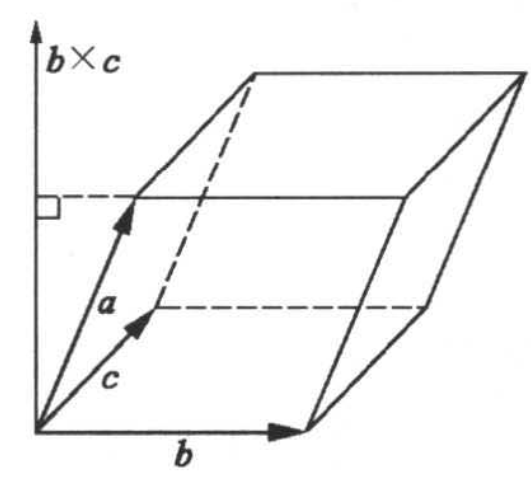
\includegraphics[width=\textwidth]{6.1.png} % 无需重复指定宽度  
\end{myimagebox}     
\caption{\label{fig:6.1}混合积的几何意义}   
\end{figure}

根据混合积的几何意义,我们可以得到如下公式:
\begin{align*}
\bm{a}\cdot(\bm{b}\times\bm{c})=\bm{c}\cdot(\bm{a}\times\bm{b})=\bm{b}\cdot(\bm{c}\times\bm{a})\tag{6-4}
\end{align*}

在这个等式中,将三个向量的位置轮换交换,其混合积的结果不变。显然如果三个向量共面,则混合积为0。

\textbf{例}:对于任意的两个向量$\bm{a},\bm{b}$,证明:
\begin{align*}
    (\bm{a}\times\bm{b})^2+(\bm{a}\cdot\bm{b})^2=|\bm{a}|^2|\bm{b}|^2
\end{align*}

\textbf{解}:直接带入向量内积和外积的定义:
\begin{align*}
    (\bm{a}\times\bm{b})^2+(\bm{a}\cdot\bm{b})^2&=|\bm{a}|^2|\bm{b}|^2\sin^2\theta+|\bm{a}|^2|\bm{b}|^2+\cos^2\theta\\
    &=|\bm{a}|^2|\bm{b}|^2
\end{align*}

\subsubsection{向量的空间坐标}
在高中我们学习过空间直角坐标系,那么我们对一个三个实数所组成的有序数组$(x,y,z)$,其可以对应到空间的一个点。而空间的一个点$P$又可以对应到向量$\bm{OP}$,因此我们可以将点$P$的坐标$(x,y,z)$对应到向量的坐标。假设$x,y,z$轴方向上的单位向量为$\bm{i},\bm{j},\bm{k}$,则$\bm{OP}$的坐标$(x,y,z)$就等价于:
\begin{align*}
    \bm{OP}=x\bm{i}+y\bm{j}+z\bm{k}
\end{align*}

记作$\bm{OP}=(x,y,z)$。根据这一定义,可以得到向量的模长可以表示为:
\begin{align*}
    |\bm{a}|=\sqrt{x^2+y^2+z^2}
\end{align*}

因此沿着$\bm{a}$方向的单位向量$\bm{a^0}$可以表示为:
\begin{align*}
    \bm{a^0}=\frac{(x,y,z)}{\sqrt{x^2+y^2+z^2}}
\end{align*}

对于两个向量$(x_1,y_1,z_1);(x_2,y_2,z_2)$,其和向量为$(x_1+x_2,y_1+y_2,z_1+z_2)$。同样的对向量$\bm{OP}$进行数乘,新向量的表示为$(\lambda x,\lambda y,\lambda z)$。

接下来我们说明在直角坐标系中向量外积和内积的坐标表示。设向量$\bm{a_1}=(x_1,y_1,z_1),\bm{a_2}=(x_2,y_2,z_2)$,则:
\begin{align*}
    \bm{a_1}&=x_1\bm{i}+y_1\bm{j}+z_1\bm{k}\\
    \bm{a_2}&=x_2\bm{i}+y_2\bm{j}+z_2\bm{k}
\end{align*}

考虑到两个向量的内积表示:由于$\bm{i}\cdot\bm{j}=\delta_{ij}$,因此:
\begin{tcolorbox}[
    colback=bac1,     % 极浅黄色背景
    colframe=fra1,   % 浅黄色边框
    coltitle=white,             % 标题文字白色
    coltext=tex1,
    title=内积的坐标表示,
    fonttitle=\bfseries,        % 标题加粗
arc=3mm,                     % 圆角稍大
breakable
]
向量内积的坐标表示为:
\begin{align*}
    \bm{a_1}\cdot\bm{a_2}=x_1x_2+y_1y_2+z_1z_2\tag{6-5}
\end{align*}
\end{tcolorbox}

接下来我们介绍向量的外积。对于二阶行列式和三阶行列式的计算,可以查阅我的《线性代数B》讲义或者高数课本。对于外积,由于$\bm{i}\times\bm{i}=\bm{j}\times\bm{j}=\bm{k}\times\bm{k}=\bm{0}$,并且$\bm{i}\times\bm{j}=\bm{k},\bm{k}\times\bm{j}=\bm{i},\bm{k}\times\bm{i}=\bm{j}$。因此向量的内积可以表示为:
\begin{align*}
    \bm{a_1}\times\bm{a_2}=(y_1z_2-z_1y_2)\bm{i}+(z_1x_2-x_1z_2)\bm{j}+(x_1y_2-y_1x_2)\bm{k}
\end{align*}

\begin{tcolorbox}[
    colback=bac1,     % 极浅黄色背景
    colframe=fra1,   % 浅黄色边框
    coltitle=white,             % 标题文字白色
    coltext=tex1,
    title=外积的坐标表示,
    fonttitle=\bfseries,        % 标题加粗
arc=3mm,                     % 圆角稍大
breakable
]
向量外积的坐标用行列式可以表示表示为:
\begin{align*}
    \bm{a_1}\times\bm{a_2}=\begin{vmatrix}
\bm{i}  & \bm{j} & \bm{k} \\
 x_1 & y_1 & z_1\\
 x_2 &y_2  & z_2
\end{vmatrix}\tag{6-6}
\end{align*}
\end{tcolorbox}

最后我们介绍\textbf{方向余弦}的概念。设$\bm{a}$是一个非零向量,其与$x,y,z$轴的夹角为$\alpha,\beta,\gamma\in[0,\pi]$。那么称这三个角为$\bm{a}$的方向角,称$\cos\alpha,\cos\beta,\cos\gamma$为向量$\bm{a}$的方向余弦。根据这个定义,我们有:
\begin{align*}
    \cos\alpha=\frac{\bm{a}\cdot\bm{i}}{|\bm{a}|}=\frac{x}{\sqrt{x^2+y^2+z^2}}\\
\cos\beta=\frac{\bm{a}\cdot\bm{j}}{|\bm{a}|}=\frac{y}{\sqrt{x^2+y^2+z^2}}\\
\cos\gamma=\frac{\bm{a}\cdot\bm{k}}{|\bm{a}|}=\frac{z}{\sqrt{x^2+y^2+z^2}}\tag{6-7} 
\end{align*}

显然根据方向余弦的定义,可以得到$\cos^2\alpha+\cos^2\beta+\cos^2\gamma=1$。

\textbf{例}:设$|\bm{a}|=\sqrt{2}$,且方向角满足$\alpha=\beta=\frac{1}{2}\gamma$,求$\bm{a}$的坐标。

\textbf{解}:由条件,$x=y=\frac{1}{2}z$,联立$\sqrt{x^2+y^2+z^2}=\sqrt{2}$得到,$x=y=\frac{\sqrt{3}}{3}$,$z=\frac{2\sqrt{3}}{3}$。

\subsection{空间解析几何}
\subsubsection{空间中直线和平面的方程}
平面的方程表示方法有很多,我们主要介绍\textbf{点法式方程,三点式方程,截距式方程}。

假设给定了一个平面,其法向量为$\bm{n}$(垂直于平面的向量称作法向量),其坐标为$(A,B,C)$。又假设该平面上一点$P_0$的坐标为$(x_0,y_0,z_0)$,则这个平面将是满足下列条件的点$P$的集合:点$P(x,y,z)$与$P_0$连接的向量与法向量垂直,即就是$\bm{n}\cdot\bm{PP_0}=0$。因此方程的表达式为:
\begin{align*}
    A(x-x_0)+B(y-y_0)+C(z-z_0)=0
\end{align*}
\begin{tcolorbox}[
    colback=bac1,     % 极浅黄色背景
    colframe=fra1,   % 浅黄色边框
    coltitle=white,             % 标题文字白色
    coltext=tex1,
    title=平面的点法式方程,
    fonttitle=\bfseries,        % 标题加粗
arc=3mm,                     % 圆角稍大
breakable
]
将上面的结果进一步化简,可以得到平面的点法式方程:
\begin{align*}
    Ax+By+Cz+D=0\tag{6-8}
\end{align*}

我们发现,这个平面的一个法向量可以直接看这个方程的参数就可以得到,这个结论是非常重要的。我们把这个三元一次方程也称作平面的一般方程。
\end{tcolorbox}

\textbf{例:}已知一个平面的方程为$Ax+By+Cz+D=0$,其中$A^2+B^2+C^2\neq 0$。求点$P_1(x_1,y_1,z_1)$到该平面的距离$d$。

\textbf{解:}这道例题的结论是非常重要的。我们假设$P_1$到该平面的垂足为$P_2$。那么所求的距离就是$\bm{P_1P_2}$的模长。又设$P_0(x_0,y_0,z_0)$为任意平面一点,则$D=-Ax_0-By_0-Cz_0$。画图可得$d=|\bm{P_0P_1}||\cos<\bm{n},\bm{P_0P_1}>|$,于是:
\begin{align*}
    d=\frac{|\bm{P_0P_1}\cdot\bm{n}|}{\bm{n}}=\frac{|Ax_1+By_1+Cz_1+D|}{\sqrt{A^2+B^2+C^2}}\tag{6-9}
\end{align*}

接下来我们看平面的三点式方程。假设平面过三个点$P_1(x_1,y_1,z_1);P_2(x_2,y_2,z_2);P_3(x_3,y_3,z_3)$,这三个点不共线的时候才能确定一个平面。那么点$P$应该是满足下面条件的点的集合:点$P$与三个点连接形成三个向量的混合积为0,即就是$\bm{P_1P}\cdot(\bm{P_2P}\times\bm{P_3P})=0$。

\begin{tcolorbox}[
    colback=bac1,     % 极浅黄色背景
    colframe=fra1,   % 浅黄色边框
    coltitle=white,             % 标题文字白色
    coltext=tex1,
    title=平面的三点式方程,
    fonttitle=\bfseries,        % 标题加粗
arc=3mm,                     % 圆角稍大
breakable
]
写成行列式形式就得到了平面的三点式方程:
\begin{align*}
\begin{vmatrix}
 x-x_1 & y-y_1 & z-z_1\\
x_2-x_1  & y_2-y_1  &z_2-z_1 \\
  x_3-x_1 & y_3-y_1  & z_3-z_1
\end{vmatrix}=0\tag{6-10} 
\end{align*}
\end{tcolorbox}

我们接下来考虑一些特殊的平面。假设在平面的一般方程$Ax+By+Cz+D=0$中,$A=B=0$。那么法向量就是$(0,0,C)$,也就是说这个平面与$Oxy$平面平行。假设$A=0$,那么法向量$(A,B,C)$与$x$轴垂直。

\begin{tcolorbox}[
    colback=bac1,     % 极浅黄色背景
    colframe=fra1,   % 浅黄色边框
    coltitle=white,             % 标题文字白色
    coltext=tex1,
    title=平面的截距式方程,
    fonttitle=\bfseries,        % 标题加粗
arc=3mm,                     % 圆角稍大
breakable
]
如果现在平面与三个轴都不垂直并且不过原点,那么将6-8变形可以得到:
\begin{align*}
    \frac{x}{-D/A}+\frac{y}{-D/B}+\frac{z}{-D/C}=1\tag{6-11}
\end{align*}

这个方程称作平面的截距式方程。因为分母都是与坐标轴的截距。例如一个平面与三个坐标轴的交点为$(1,0,0);(0,2,0);(0,0,3)$,那么平面方程可以写作$\frac{x}{1}+\frac{y}{2}+\frac{z}{3}=0$。
\end{tcolorbox}

接下来我们讨论如何根据两个平面的方程确定两个平面的位置和相交时的夹角。我们考虑两个平面$A_1x+B_1y+C_1z+D_1=0,A_2x+B_2y+C_2z+D_2=0$。由于这两个平面的法向量为$(A_1,B_1,C_1);(A_2,B_2,z_2)$。这\textbf{两个平面平行的充要条件应该是这两个法向量平行}。因此就有:
\begin{align*}
    (A_1,B_1,C_1)=\lambda(A_2,B_2,C_2)\qquad \lambda\neq 0\tag{6-12}
\end{align*}

而两个平面之间的夹角就是法向量之间的夹角,可以计算得到:
\begin{align*}
    \cos\theta=\frac{A_1A_2+B_1B_2+C_1C_2}{\sqrt{(A_1^2+B_1^2+C_1^2)(A_2^2+B_2^2+C_2^2)}}
\end{align*}

当$\theta=90^\circ$时,平面相互垂直,此时:
\begin{align*}
    A_1A_2+B_1B_2+C_1C_2=0\tag{6-13}
\end{align*}

接下来我们讨论空间直线的方程。在空间内一条直线的方程要通过两个平面方程去描述。直线总可以看做两个不平行平面的交线,换言之直线上的点是下列方程组的解:
\begin{align*}
    \begin{cases}
        A_1x+B_1y+C_1z+D_1=0\\
        A_2x+B_2y+C_2z+D_2=0
    \end{cases}
\end{align*}

当然这两个平面不平行。这种形式称作直线的\textbf{一般方程}。接下来我们讨论直线的参数方程:

假设已知一点$P_0(x_0,y_0,z_0)$和一个非零向量$\bm{e}=(a,b,c)$。那么过$P_0$且方向与$\bm{e}$平行的直线上任意一点$\bm{P}(x,y,z)$都使得向量$\bm{P_0P}$与向量$\bm{e}$贡献。即就是存在一个实数$t$满足:
\begin{align*}
    \bm{P_0P}=t\bm{e}\to x-x_0=ta;y-y_0=tb;z-z_0=tc
\end{align*}

\begin{tcolorbox}[
    colback=bac1,     % 极浅黄色背景
    colframe=fra1,   % 浅黄色边框
    coltitle=white,             % 标题文字白色
    coltext=tex1,
    title=直线的参数方程,
    fonttitle=\bfseries,        % 标题加粗
arc=3mm,                     % 圆角稍大
breakable
]
这组方程称作直线的参数方程。非零向量$\bm{e}$称作直线的方向向量。从参数方程出发消去参数$t$能得到下面的\textbf{标准方程}:
\begin{align*}
    \frac{x-x_0}{a}=\frac{y-y_0}{b}=\frac{z-z_0}{c}\tag{6-14}
\end{align*}
\end{tcolorbox}

\subsubsection{二次曲面}
在上一节我们知道,一个三元一次方程在空间中可以代表一个平面。而在本章我们说明,如下形式的三元二次方程:
\begin{align*}
    Ax^2+By^2+Cz^2+Dxy+Exz+Fyz+Gx+Hy+Iz+J=0
\end{align*}

可以代表空间中的一个曲面。而通过合适的坐标代换(不在本课程讨论范围之内)可以将其转化为下面的9种基本二次曲面。本章的目的是在于了解这9种基本二次曲面的解析式和图像,读者只需能根据图象和解析式分辨二次曲面的种类即可。

1:\textbf{椭圆锥面}:其解析式和图象如下:
\begin{align*}
    \frac{x^2}{a^2}+\frac{y^2}{b^2}-\frac{z^2}{c^2}=0\tag{6-15}
\end{align*}
\begin{figure}[H]    
\centering     
\renewcommand{\figurename}{图}     
\renewcommand{\thefigure}{6.2}    
\begin{myimagebox}[width=0.23\textwidth] % 直接传入图片尺寸参数      
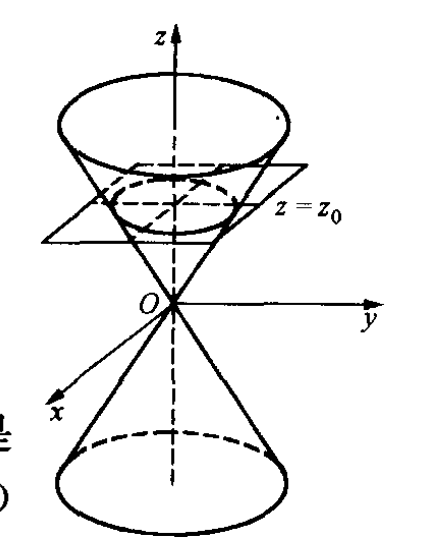
\includegraphics[width=\textwidth]{6.2.png} % 无需重复指定宽度  
\end{myimagebox}     
\caption{\label{fig:6.2}椭圆锥面的图象}   
\end{figure}

当确定$z=z_0$时,平面图像为$\frac{x^2}{a^2}+\frac{y^2}{b^2}=\frac{z_0^2}{c^2}$,截面是一个椭圆。此外与$Oyz$平面与$Ozx$平面截取出来的都是两条直线。

2:\textbf{椭球面},其解析式和图象如下:
\begin{align*}
    \frac{x^2}{a^2}+\frac{y^2}{b^2}+\frac{z^2}{c^2}=1\tag{6-16}
\end{align*}

其可以使用参数方程表示:
\begin{align*}
    x=a\sin\varphi\cos\theta\qquad y=b\sin\varphi\sin\theta\qquad z=c\cos\varphi\tag{6-17}
\end{align*}
\begin{figure}[H]    
\centering     
\renewcommand{\figurename}{图}     
\renewcommand{\thefigure}{6.3}    
\begin{myimagebox}[width=0.23\textwidth] % 直接传入图片尺寸参数      
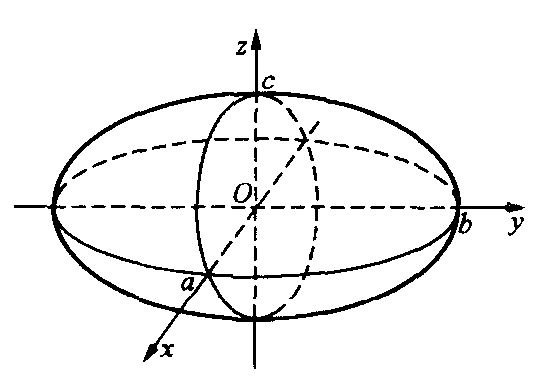
\includegraphics[width=\textwidth]{6.3.png} % 无需重复指定宽度  
\end{myimagebox}     
\caption{\label{fig:6.3}椭球面的图象}   
\end{figure}

3:\textbf{单叶双曲面},其解析式和图象如下:
\begin{align*}
    \frac{x^2}{a^2}+\frac{y^2}{b^2}-\frac{z^2}{c^2}=1\tag{6-18}
\end{align*}
\begin{figure}[H]    
\centering     
\renewcommand{\figurename}{图}     
\renewcommand{\thefigure}{6.4}    
\begin{myimagebox}[width=0.23\textwidth] % 直接传入图片尺寸参数      
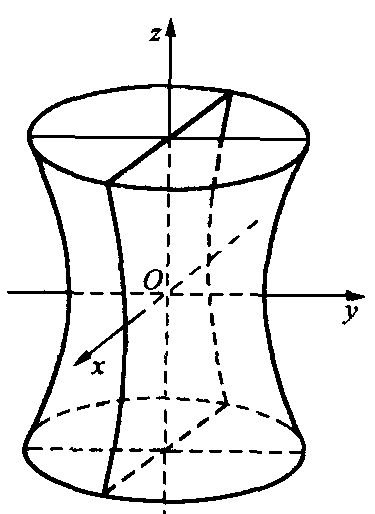
\includegraphics[width=\textwidth]{6.4.png} % 无需重复指定宽度  
\end{myimagebox}     
\caption{\label{fig:6.4}单页双曲面的图象}   
\end{figure}

用平面$z=z_0$截取这个平面,截面是一个椭圆周。用平面$z=z_0$或者$y=y_0$截取时,截痕是双曲线。

4:\textbf{双叶双曲面},其解析式和图象如下:
\begin{align*}
    \frac{x^2}{a^2}+\frac{y^2}{b^2}-\frac{z^2}{c^2}=-1\tag{6-19}
\end{align*}

\begin{figure}[H]    
\centering     
\renewcommand{\figurename}{图}     
\renewcommand{\thefigure}{6.5}    
\begin{myimagebox}[width=0.23\textwidth] % 直接传入图片尺寸参数      
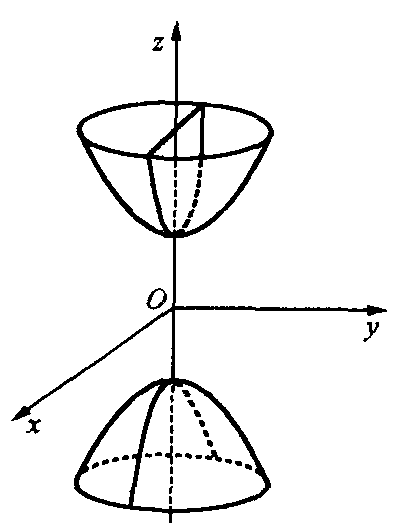
\includegraphics[width=\textwidth]{6.5.png} % 无需重复指定宽度  
\end{myimagebox}     
\caption{\label{fig:6.5}双页双曲面的图象}   
\end{figure}
与单叶双曲面不同,它在$z\in [-c,c]$区间上是没有图象的。

5:\textbf{椭圆柱面},其解析式和图象如下:
\begin{align*}
    \frac{x^2}{a^2}+\frac{y^2}{b^2}=1\tag{6-20}
\end{align*}
\begin{figure}[H]    
\centering     
\renewcommand{\figurename}{图}     
\renewcommand{\thefigure}{6.6}    
\begin{myimagebox}[width=0.23\textwidth] % 直接传入图片尺寸参数      
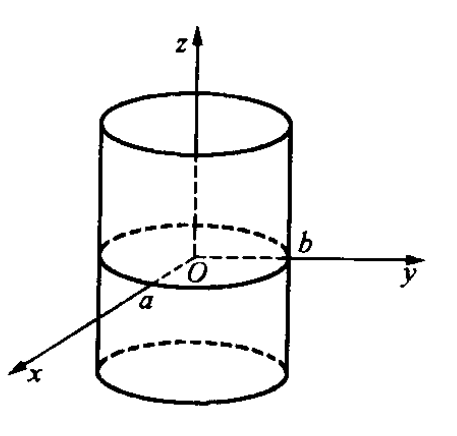
\includegraphics[width=\textwidth]{6.6.png} % 无需重复指定宽度  
\end{myimagebox}     
\caption{\label{fig:6.6}椭圆柱面的图象}   
\end{figure}

6:\textbf{双曲柱面},其解析式和图象如下:
\begin{align*}
    \frac{x^2}{a^2}-\frac{y^2}{b^2}=1\tag{6-21}
\end{align*}
\begin{figure}[H]    
\centering     
\renewcommand{\figurename}{图}     
\renewcommand{\thefigure}{6.7}    
\begin{myimagebox}[width=0.23\textwidth] % 直接传入图片尺寸参数      
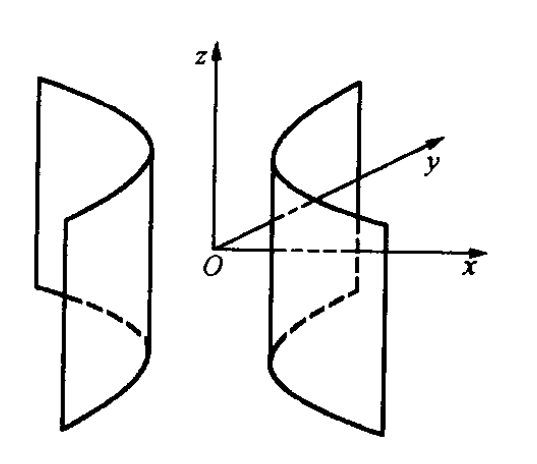
\includegraphics[width=\textwidth]{6.7.png} % 无需重复指定宽度  
\end{myimagebox}     
\caption{\label{fig:6.7}双曲柱面的图象}   
\end{figure}

7:\textbf{椭圆抛物面},其解析式和图象如下:
\begin{align*}
    \frac{x^2}{a^2}+\frac{y^2}{b^2}-z=0\tag{6-22}
\end{align*}

\begin{figure}[H]    
\centering     
\renewcommand{\figurename}{图}     
\renewcommand{\thefigure}{6.8}    
\begin{myimagebox}[width=0.23\textwidth] % 直接传入图片尺寸参数      
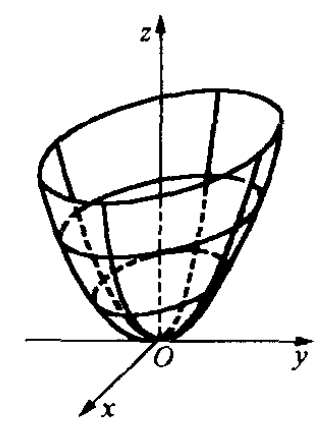
\includegraphics[width=\textwidth]{6.8.png} % 无需重复指定宽度  
\end{myimagebox}     
\caption{\label{fig:6.8}椭圆抛物面的图象}   
\end{figure}

8:\textbf{双曲抛物面},其解析式和图象如下:
\begin{align*}
    \frac{x^2}{a^2}-\frac{y^2}{b^2}-z=0\tag{6-23}
\end{align*}
\begin{figure}[H]    
\centering     
\renewcommand{\figurename}{图}     
\renewcommand{\thefigure}{6.9}    
\begin{myimagebox}[width=0.23\textwidth] % 直接传入图片尺寸参数      
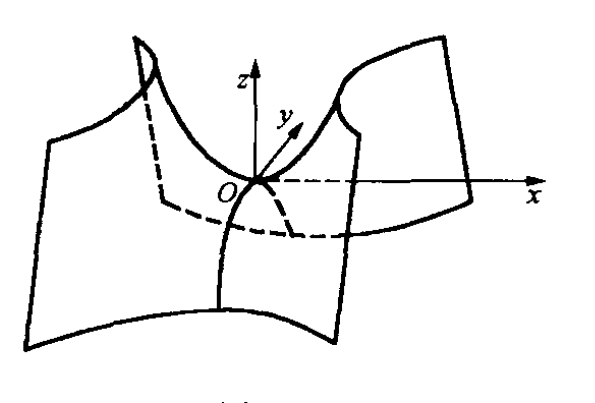
\includegraphics[width=\textwidth]{6.9.png} % 无需重复指定宽度  
\end{myimagebox}     
\caption{\label{fig:6.9}双曲抛物面的图象}   
\end{figure}

9:\textbf{抛物柱面},其解析式和图象如下:
\begin{align*}
    \frac{x^2}{a}-y=0\tag{6-24}
\end{align*}
\begin{figure}[H]    
\centering     
\renewcommand{\figurename}{图}     
\renewcommand{\thefigure}{6.10}    
\begin{myimagebox}[width=0.23\textwidth] % 直接传入图片尺寸参数      
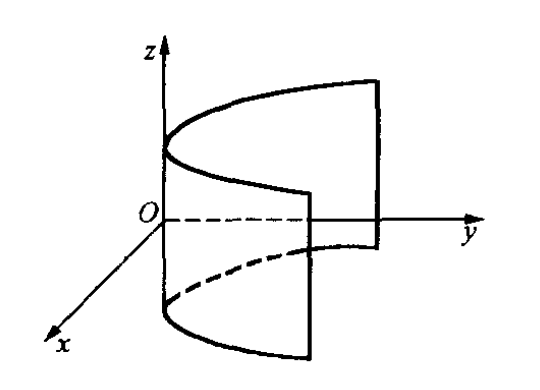
\includegraphics[width=\textwidth]{6.10.png} % 无需重复指定宽度  
\end{myimagebox}     
\caption{\label{fig:6.10}抛物柱面的图象}   
\end{figure}

\subsubsection{空间曲线的切线与弧长}
在立体空间中,我们可以用参数方程的形式给出一条曲线的解析式:
\begin{align*}
    x=x(t) \quad  y=y(t)\quad z=z(t)\qquad t\in[a,b]
\end{align*}

如果空间内的点$P(x,y,z)$可以用向量$\bm{r}=\bm{OP}$表示,那么上述的空间曲线就可以用一个\textbf{向量函数}表示:
\begin{align*}
    \bm{r}(t)=x(t)\bm{i}+y(t)\bm{j}+z(t)\bm{k}\tag{6-25}
\end{align*}

如果$x(t),y(t),z(t)$在$t\in[a,b]$上有连续导数并且三个导数不同时为0,则称曲线是一条光滑曲线。

接下来我们定义\textbf{向量函数的导数}。根据导数的定义,我们做如下的计算:
\begin{align*}
\bm{r}'(t)&=\frac{\bm{r}(t+\Delta t)-\bm{r}(t)}{\Delta t}\\
&=\lim_{\Delta t\to 0}\frac{x(t+\Delta t)-x(t)}{\Delta t}\bm{i}+
\frac{y(t+\Delta t)-y(t)}{\Delta t}\bm{j}  +\frac{z(t+\Delta t)-z(t)}{\Delta t}\bm{k}\\
&=x'(t)\bm{i}+y'(t)\bm{j}+z'(t)\bm{k}\tag{6-26} 
\end{align*}

而在几何意义上,$\bm{r}'(t)$代表了切线的方向。光滑曲线在点$\bm{r}'(t_0)$的切线方程为:
\begin{align*}
    \bm{r}=\bm{r}(t_0)+u\bm{r'}(t_0)
\end{align*}

\begin{tcolorbox}[
    colback=bac1,     % 极浅黄色背景
    colframe=fra1,   % 浅黄色边框
    coltitle=white,             % 标题文字白色
    coltext=tex1,
    title=曲线切线方程,
    fonttitle=\bfseries,        % 标题加粗
arc=3mm,                     % 圆角稍大
breakable
]
把上面的式子改写为标准形式为:
\begin{align*}
    \frac{x-x(t_0)}{x'(t_0)}=\frac{y-y(t_0)}{y'(t_0)}=\frac{z-z(t_0)}{z'(t_0)}\tag{6-27}
\end{align*}
\end{tcolorbox}

过点$\bm{r}(t_0)$且与该点处切向量垂直的平面称作曲线在该点处的\textbf{法平面}。法平面方程为:
\begin{align*}
    x'(t_0)(x-x(t_0))+y'(t_0)(y-y(t_0))+z'(t_0)(z-z(t_0))=0\tag{6-28}
\end{align*}

而曲线的弧长计算同在定积分的应用一致,弧微元为:
\begin{align*}
    \mathrm{d}s=\sqrt{x'(t)^2+y'(t)^2+z'(t)^2}\mathrm{d}t\tag{6-29}
\end{align*}


\textbf{例}:求曲线:
\begin{align*}
    x=a\cos t\quad y=a\sin t\quad z=bt \quad(a,b>0t\in[0,\pi])
\end{align*}

在$(0,a,\frac{b\pi}{2})$的切线方程与法平面方程,并计算弧长$s$。

\textbf{解}:我们计算在这一点的切向量,由于$t=\frac{\pi}{2}$,因此切向量为$(-a,0,b)$,于是切线方程为:
\begin{align*}
    \frac{x-0}{-a}=\frac{y-a}{0}=\frac{z-\frac{b\pi}{2}}{b}
\end{align*}

法平面方程为:
\begin{align*}
    -a(x-0)+b(z-\frac{\pi}{b})=0
\end{align*}

利用弧微分计算弧长:
\begin{align*}
    s=\int_0^\pi\sqrt{a^2\sin t^2+a^2\cos t^2+b^2}\mathrm{d}t=\pi\sqrt{a^2+b^2}
\end{align*}

\section{多元函数微分学}
\subsection{多元函数的定义与性质}
\subsubsection{多元函数的定义}
我们将两个自变量形成的有序数组看成平面上的一个点,而降三个自变量的有序数组看成空间内的一个点。当一个二元函数的两个自变量在一定的允许范围内变化时,相应的有序数组对应平面上某个点的集合;对于三元函数,自变量对应空间内点的集合。那么一个二元函数实质上是平面上点的集合$D$到实数集的一个映射。同理一个三元函数本质上是空间上点的集合$\Omega$到实数集的一个映射。因此我们给出如下定义:
\begin{tcolorbox}[
    colback=bac2,     % 极浅黄色背景
    colframe=fra2,   % 浅黄色边框
    coltitle=white,             % 标题文字白色
    coltext=tex2,
    title=多元函数的定义,
    fonttitle=\bfseries,        % 标题加粗
arc=3mm,                     % 圆角稍大
breakable
]
设有一个集合$D\subset \mathbb{R}^n$,若对于$D$内的每一点$(x_1,x_2...x_n)$,按照一定的法则$f$,都有唯一确定的数$u\in\mathbb{R}$与之相对应,则称$f$是定义在区域$D$上的一个\textbf{$n$元函数}。区域$D$称函数$f$的\textbf{定义域}。$u$称作函数的值,全体函数值组成的集合称作函数的\textbf{值域},把$(x_1,x_2...x_n)$称作函数的\textbf{自变量}。
\end{tcolorbox}

下图展示了二元函数$f(x)=\sqrt{4-x^2-y^2}$的图象,根据图象我们得知这个函数的定义域为$D:x^2+y^2\leq 4$,值域为$[0,2]$。

\begin{figure}[H]    
\centering     
\renewcommand{\figurename}{图}     
\renewcommand{\thefigure}{7.1}    
\begin{myimagebox}[width=0.5\textwidth] % 直接传入图片尺寸参数      
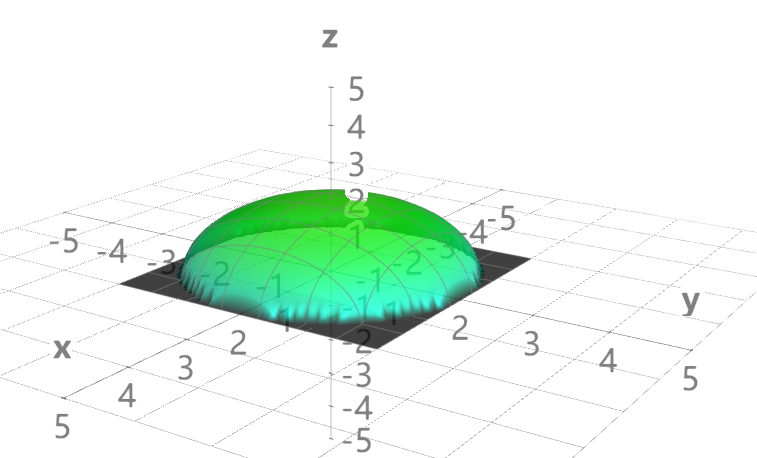
\includegraphics[width=\textwidth]{7.1.png} % 无需重复指定宽度  
\end{myimagebox}     
\caption{\label{fig:7.1}多元函数的图象}   
\end{figure}

然而上述函数最重视映射到$\mathbb{R}$的,当然多元函数的映射关系也可以是映射到$\mathbb{R}^m$的,例如平面坐标变换:
\begin{align*}
    \begin{cases}
u=x\cos\alpha-y\sin\alpha\\
v=x\sin\alpha+y\cos\alpha
    \end{cases}
\end{align*}

可以理解为是$(x,y)\in\mathbb{R}^2$映射到$(u,v)\in\mathbb{R}^2$的一个函数。因此我们可以进一步丰富多元函数的定义:

\begin{tcolorbox}[
    colback=bac2,     % 极浅黄色背景
    colframe=fra2,   % 浅黄色边框
    coltitle=white,             % 标题文字白色
    coltext=tex2,
    title=多元函数的定义,
    fonttitle=\bfseries,        % 标题加粗
arc=3mm,                     % 圆角稍大
breakable
]
设$D$是$\mathbb{R}^n$中的一个集合,又设$\bm{f}$是$D\to\mathbb{R}^m$的一个映射,则对于$D$中的每一点$(x_1,x_2..x_n)$在$\mathbb{R}^m$中都有唯一确定的一点$(y_1,y_2...y_m)$与之对应,那么这个映射$f$相当于具有$m$个分量的$n$元函数,即就是:
\begin{align*}
    y_i=f_i(x_1,x_2,...x_n)
\end{align*}
\end{tcolorbox}

接下来我们需要定义在$\mathbb{R}^n$中有关距离,邻域,开集的概念。在$n$维实数空间中,点$P(x_1,x_2...x_n)$到点$P_0(x_1^0,x_2^0...x_n^0)$的距离为:
\begin{align*}
    d(P,Q)=\sqrt{\sum_{j=1}^n(x_j-x_j^0)^2}\tag{7-1}
\end{align*}

那么对于这个距离$d(P,Q)$就有这样的几条性质:

\begin{enumerate}
    \item $d(P,Q)\geq 0$。当且仅当$P,Q$重合时等号成立。
    \item $d(P,Q)=d(Q,P)$
    \item $d(P,Q)\leq d(P,R)+d(R,Q)$(\textbf{三角不等式})
\end{enumerate}

定义了距离之后,我们就可以定义邻域的概念:
\begin{tcolorbox}[
    colback=bac2,     % 极浅黄色背景
    colframe=fra2,   % 浅黄色边框
    coltitle=white,             % 标题文字白色
    coltext=tex2,
    title=邻域的定义,
    fonttitle=\bfseries,        % 标题加粗
arc=3mm,                     % 圆角稍大
breakable
]
设$P_0\in\mathbb{R}^n$为给定的一点,$r$是给定的一个整数,我们定义点$P_0$的邻域是集合:
\begin{align*}
    U_r(P_0)=\{ P\in\mathbb{R}^n|d(P,P_0)<r\}
\end{align*}
\end{tcolorbox}

当$n=3$时,邻域是一个\textbf{开球}(因为不包含球面);$n=2$时邻域是一个\textbf{开圆}。接下来我们定义开集和区域的概念。

设$E\subset \mathbb{R}^n$时一个给定的集合。根据集合$E$,我们把空间的点分作三类:$E$的内点,外点和临界点。一点$P\in\mathbb{R}^n$如果存在一个正数$r$使得$U_r(P)\subset E$(邻域全部在集合内),那么成这个点为$E$的\textbf{内点}。而如果存在一个整数$r$使得$U_r(P)\cap E=\emptyset$,那么成这个点是\textbf{外点}。不是内点也不是外点的点统称为边界点。$\partial E$是集合$E$所有边界点的集合,称作$E$的\textbf{边界}。

如果一个集合$E$的每一点都是内点,那么称作\textbf{开集}。集合$E$是开集的充要条件是集合$E$没有边界点。一个集合$E$如果包含所有的边界点,那么称集合$E$是\textbf{闭集}。开集和闭集是两种极端情况,只包含部分边界点的集合既不是开集也不是闭集。

如果集合$E$任意两点都可以用一条落在$E$内的曲线相连接,我们称$E$是连通的。$\mathbb{R}^n$中\textbf{连通的非空开集称作区域}。

设$G$是一个区域,那么集合$G\cup\partial G$就是一个闭集,记作$\bar{G}$,称作\textbf{闭区域}。

如果存在一个正数$\rho$,使得$E$包含于以原点为中心,$\rho$为半径的球内,那么称$E$是\textbf{有界集合},反之为\textbf{无界集合}。

\subsubsection{多元函数的极限与连续性}
我们在以后对于新概念的叙述与二元函数为例,多元函数的情况类似。对于一个一元函数,我们讨论的极限是自变量$x$在$x$轴上以两个方向趋近于考察点$x_0$处函数值的情况。但对于一个二元函数呢?

二元函数的情况类似,正如图$7.1$所示。我们考虑这个多元函数在点$(0,0)$处的极限。那么我们实际上考察自变量组$(x,y)$在$Oxy$平面上趋近于$(0,0)$时的情况。不过与一元函数不同的是,\textbf{我们考察的极限是从“四面八方”趋近的而不是只从坐标轴趋近的},因此我们给出极限的定义:
\begin{tcolorbox}[
    colback=bac2,     % 极浅黄色背景
    colframe=fra2,   % 浅黄色边框
    coltitle=white,             % 标题文字白色
    coltext=tex2,
    title=二元函数的极限,
    fonttitle=\bfseries,        % 标题加粗
arc=3mm,                     % 圆角稍大
breakable
]
设函数$f(x,y)$在点$(x_0,y_0)$的某个空心邻域内有定义,若有一个常数$A$,对于任意给定的$\varepsilon>0$,都存在一个$\delta>0$,使得当$0<\sqrt{(x-x_0)^2+(y-y_0)^2}<\delta$时,都有$|f(x,y)-A|<\varepsilon$。则称当点$(x,y)$趋近于$(x_0,y_0)$时,$f(x,y)$\textbf{以$A$为极限}。记作:
\begin{align*}
    \lim_{(x,y)\to(x_0,y_0)}f(x;y)=A\tag{7-2}
\end{align*}
\end{tcolorbox}

给定$P_0(x_0,y_0)$,记动点$(x,y)$为$P$,那么上述定义也可以描述成$\forall \varepsilon>0,\exists\delta>0$,使得当$P$在$P_0$的空心$\delta$邻域时,函数值$f(P)$落在点$A$的$\varepsilon$邻域内。定义1中我们用距离$d(P,P_0)<\delta$刻画了$(x,y)$充分靠近$(x_0,y_0)$。我们也可以用下面的方形区域刻画“充分靠近”的定义:
\begin{align*}
    |x-x_0|<\delta \qquad |y-y_0|<\delta 
\end{align*}

上面对于极限的定义就是多元函数极限的$N-\varepsilon$语言。我们可以利用这种方法去说明多元函数的极限。

\textbf{例}:考虑二元函数$f(x;y)=\frac{x\sin y}{\sqrt{x^2+y^2}}$,证明$\lim_{(x,y)\to(0,0)}f(x;y)=0$

\textbf{解}:根据不等式:
\begin{align*}
    |x\sin y|\leq|xy|\leq\frac{1}{2}(x^2+y^2)
\end{align*}

我们有$|f(x;y)-0|<\frac{1}{2}\sqrt{x^2+y^2}$。如果能说明右面小于$\varepsilon$即可。我们取$\delta=2\varepsilon$,则当$\sqrt{x^2+y^2}<\delta$时满足条件。因此极限证毕。

二元函数的极限性质和一元函数基本一致,存在\textbf{四则运算,比较定理,夹逼定理}。这里就不再展开。同理复合函数的极限定理也省略,同一元函数。读者可自行查阅课本。

\textbf{自行练习}:请你叙述二元函数极限唯一性定理(考虑一元函数的极限唯一性定理),并且证明之,加深对$N-\varepsilon$语言的掌握。

\textbf{解:}我们这里不再叙述定理,只对其进行证明。假设$\lim_{P\to P_0}f(x;y)=A$并且$\lim_{P\to P_0}f(x;y)=B$,则当$d(P,P_0)<\delta$时要满足:
\begin{align*}
    |f(x;y)-A|<\varepsilon\qquad |f(x;y)-B|<\varepsilon
\end{align*}

那么就会有$f(x;y)\in (A-\varepsilon,A+\varepsilon)$,也就是说$\max|f(x;y)|=\max\{|A-B-\varepsilon|,|A-B+\varepsilon|\}$。此时$A=B$。

在实际情况下,我们通常不使用$N-\varepsilon$语言。多元函数的极限计算通常有下列的办法:
\begin{enumerate}
    \item 利用函数的\textbf{连续性}和\textbf{极限计算}性质。
    \item 不等式放缩,\textbf{夹逼定理}。
    \item 通过\textbf{变量替换}转化为一元极限。
\end{enumerate}

\textbf{例}:计算下列多元函数极限。
\begin{align*}
   & (1)\lim_{(x,y)\to(0,0)}\frac{x^3+y^3}{x^2+y^2}\qquad (2)\lim_{(x,y)\to(0,0)}\frac{\sin(x^3+y^3)}{x^2+y^2}\\
    &(3)\lim_{(x,y)\to(0,0)}(x^2+y^2)^{xy}\qquad (4)\lim_{(x,y)\to (0,0)}f(x;y)=\begin{cases}
        \frac{\sin xy}{x}&x\neq 0\\
        y &x=0,y\neq 0
    \end{cases}
\end{align*}

\textbf{解}:(1)令$x=\rho\cos\theta,y=\rho\sin\theta$,显然$(x,y)\to(0,0)$的条件转化为$\rho\to 0$,因此:
\begin{align*}
    \lim_{(x,y)\to(0,0)}\frac{x^3+y^3}{x^2+y^2}=\lim_{\rho\to 0}\frac{\rho^3(\cos^3\theta+\sin^3\theta)}{\rho^2}=0
\end{align*}

(2)使用夹逼定理:
\begin{align*}
   \left| \lim_{(x,y)\to(0,0)}\frac{\sin(x^3+y^3)}{x^2+y^2}\right|\leq\lim_{(x,y)\to(0,0)}\frac{(|x|+|y|)(x^2+y^2)}{x^2+y^2}=0
\end{align*}

(3)我们先去求对数的极限$xy\ln(x^2+y^2)$。继续使用极坐标代换。
\begin{align*}
    |xy\ln(x^2+y^2)|\leq r^2\ln r^2\to 0 \quad(r\to 0+)
\end{align*}

因此二元极限为$1$。

(4)由于$|f(x;y)|\leq |y|$不管在哪种情况下都成立,因此二元极限为0。


如何证明一个二元函数极限不存在?我们想极限是要在任意的趋近路径下都要相等。因此我们只要能\textbf{找到两种趋近办法使得极限不相等,那么我们就可以说原函数极限不存在}。

例:说明当$(x,y)\to(0,0)$时,函数$\frac{|x|}{\sqrt{x^2+y^2}}$不存在极限。

\textbf{解}:考虑从$y=kx$方向逼近于$(0,0)$:
\begin{align*}
    f(x;y)=\frac{|x|}{\sqrt{x^2+k^2x^2}}=\frac{1}{\sqrt{1+k^2}}
\end{align*}

沿着不同斜率的直线趋向于原点时,函数值趋向于不同的常数,因此函数没有极限。同理,下面的二元函数在趋近于$(0,0)$时也不存在极限:
\begin{align*}
    f(x;y)=\frac{x^4y^4}{(x^2+y^4)^3}
\end{align*}

\begin{figure}[H]    
\centering     
\renewcommand{\figurename}{图}     
\renewcommand{\thefigure}{7.2}    
\begin{myimagebox}[width=0.75\textwidth] % 直接传入图片尺寸参数      
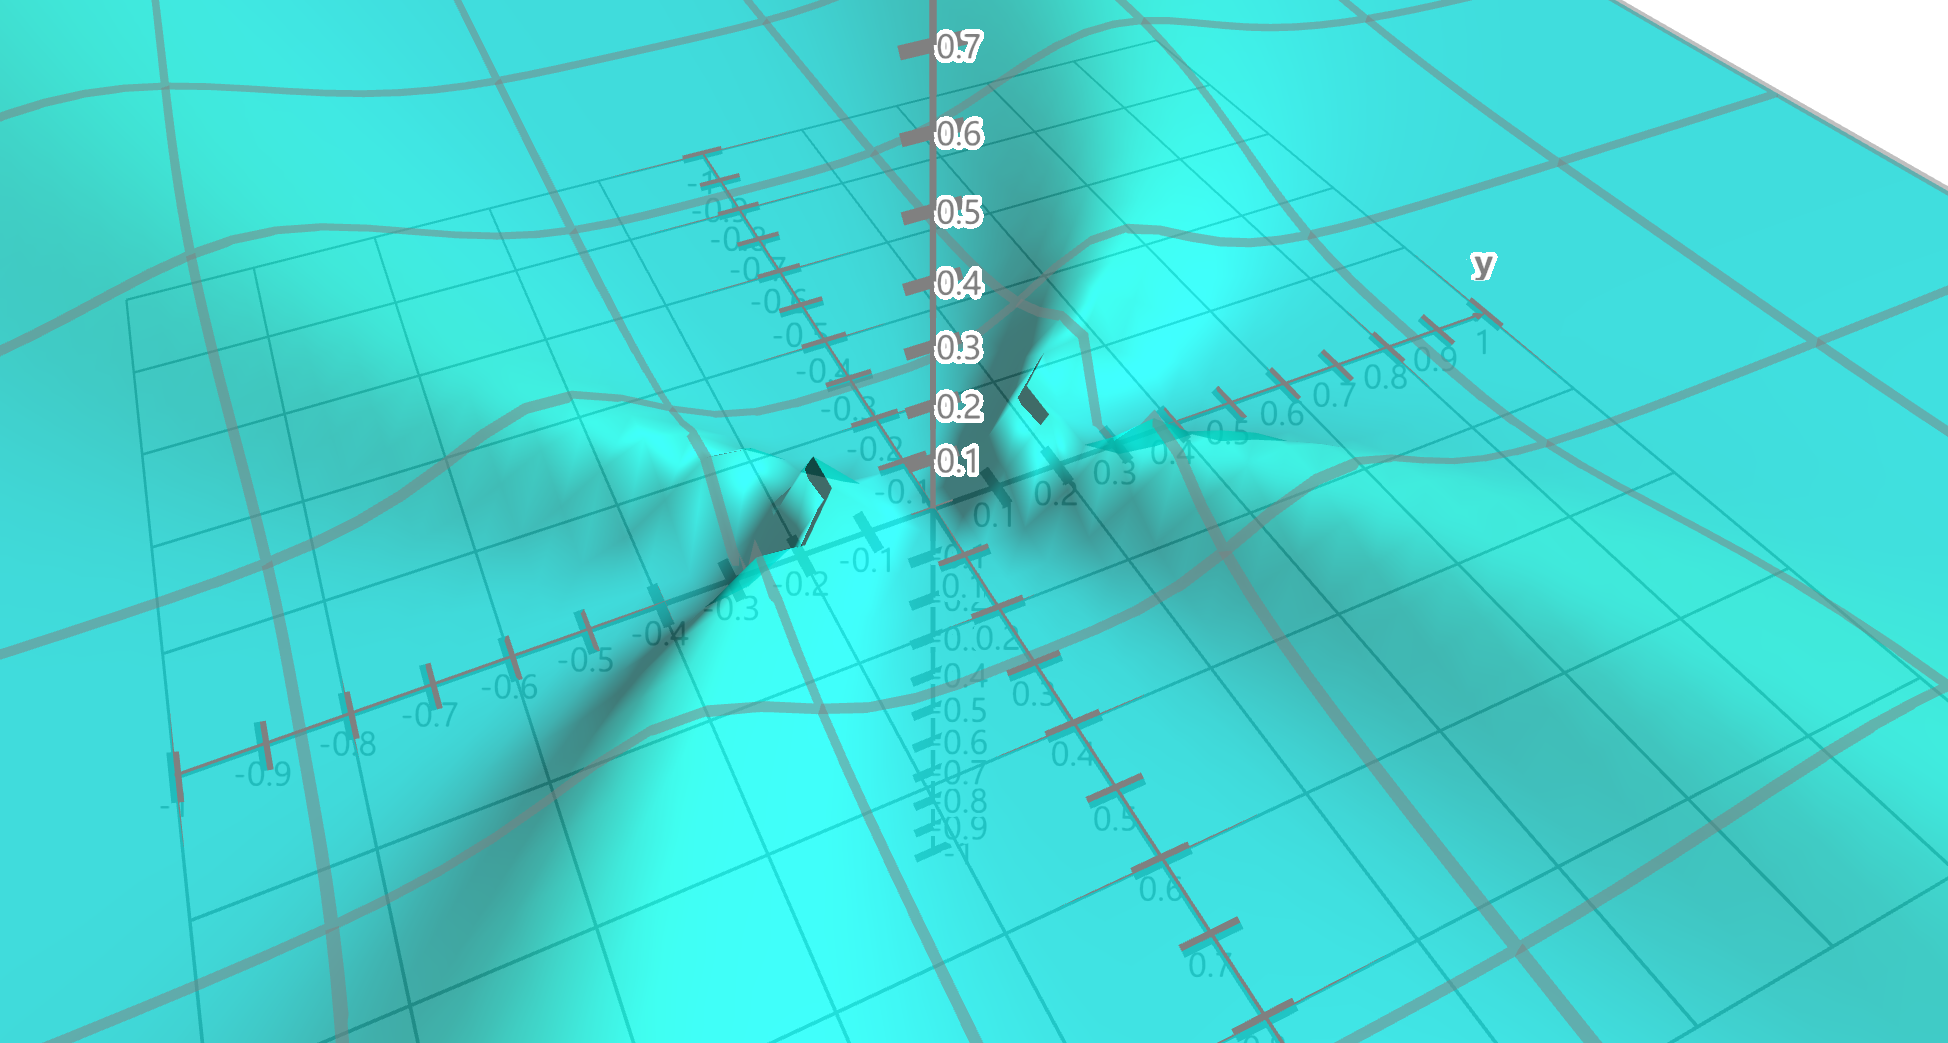
\includegraphics[width=\textwidth]{7.2.png} % 无需重复指定宽度  
\end{myimagebox}     
\caption{\label{fig:7.2}多元函数的图象}   
\end{figure}

这个函数的图象如7.2所示。如果按照$y=kx$趋近于点$(0,0)$时,函数值是趋向于$0$的,但是如果按照$y=\sqrt{x}$趋近时,函数值趋向于$\frac{1}{8}$。

最后我们补充对累次极限的讲解。一个二元函数,当其中的一个自变量$y$固定的时候,这个函数就变成了一元函数,我们可以对$x$去极限。我们假定对于固定的$y$,下面的极限存在:
\begin{align*}
    \lim_{x\to x_0}f(x;y)=g(y)
\end{align*}

那么假如此时当$y\to y_0$时,$g(y)$也存在极限,那么我们称:
\begin{align*}
    \lim_{y\to y_0}g(y)=\lim_{y\to y_0}\lim_{x\to x_0}f(x,y)
\end{align*}

称作\textbf{累次极限}。累次极限可以先$y$后$x$,也可以先$x$后$y$。例如下面的函数:
\begin{align*}
    f(x,y)=\frac{xy}{x^2+y^2}
\end{align*}

它趋向于$(0,0)$的两个累次积分都为0,但是换元$y=kx$后得到趋近于$(0,0)$的全面极限并不存在。

累次极限和全面极限的存在并没有必然联系。例如我们考察下面的函数:
\begin{align*}
    f(x;y)=\begin{cases}
        (x+y)\sin\frac{1}{x}& x\neq 0\\
        0 & x=0
    \end{cases}
\end{align*}

它的累次极限$\lim_{y\to 0}\lim_{x\to 0}f(x;y)$并不存在。因为函数$g(x)=x\sin \frac{1}{x}$在$x\to 0$不存在极限。但是全面极限是存在的。

我们定义了极限之后,就可以定义二元函数的连续性:
\begin{tcolorbox}[
    colback=bac2,     % 极浅黄色背景
    colframe=fra2,   % 浅黄色边框
    coltitle=white,             % 标题文字白色
    coltext=tex2,
    title=二元函数的连续性,
    fonttitle=\bfseries,        % 标题加粗
arc=3mm,                     % 圆角稍大
breakable
]
设函数$f(x;y)$在点$(x_0,y_0)$的一个邻域有定义,若当$(x,y)\to(x_0,y_0)$时函数$f(x,y)$有极限,且有:
\begin{align*}
    \lim_{(x,y)\to(x_0,y_0)}f(x;y)=f(x_0,y_0)
\end{align*}

则称函数$f(x,y)$在点$(x_0,y_0)$连续。如果函数在区域$D$内点点连续,称函数在区域$D$内连续。
\end{tcolorbox}

\textbf{例}:证明函数$f(x,y)=\sin(x+y)+|x+y+1|$在$\mathbb{R}^2$中任意一点处连续。

\textbf{解}:我们本质上需要使用$N-\varepsilon$语言说明:
\begin{align*}
    |\sin(x+y)|-|\sin(x_0+y_0)|&\leq 2|\sin\frac{(x+y)-(x_0+y_0)}{2}\cos\frac{(x+y)+(x_0+y_0)}{2}|\\
    \leq|x+y-x_0-y_0|\leq|x-x_0|+|y-y_0|
\end{align*}

而另一方面:
\begin{align*}
    ||x+y+1|-|x_0+y_0+1||\leq |x-x_0|+|y-y_0|
\end{align*}

因此就有:
\begin{align*}
    |f(x,y)|-f(x_0,y_0)|\leq 2|x-x_0|+2|y-y_0|
\end{align*}

如果为了使不等式右侧小于$\varepsilon$,取$\delta=\frac{1}{4}\varepsilon$即可。

\textbf{例}:说明下面的函数在定义域上是连续的:
\begin{align*}
    f(x,y)=\begin{cases}
        \frac{\ln(1+xy)}{x} & x\neq 0\\
        y &x=0
    \end{cases}
\end{align*}

\textbf{解:}显然在一切$(x_0,y_0),x_0\neq 0$处的点函数都连续。现在我们看在$(0,y_0)$处的连续性。
\begin{align*}
    |f(x,y)-f(0,y_0)|&=|y\ln(1+xy)^{1/xy}-y_0|\\
    &=|y[\ln (1+xy)^{1/xy}-1]+(y-y_0)|\\
    &\leq |y||\ln(1+xy)^{1/xy}-1|+|y-y_0|\\
    &=|y-y_0|
\end{align*}

因此取$\delta=\varepsilon$即可。

多元函数连续性的复合运算和一元函数类似,这里不再赘述。接下来我们介绍\textbf{二元初等函数}。它是从自变量$x,y$出发进行有限四则运算或者复合以一元初等函数的结果。根据一元初等函数的连续性和多元函数连续性复合运算可以得到:\textbf{二元初等函数在其定义域内连续。}

多元函数本质上是一种映射,我们之前讨论的都是二元函数$D\to\mathbb{R}$的映射,那么对于$D\to\mathbb{R}^n$的映射,其连续性该如何定义?我们做如下说明:

\begin{tcolorbox}[
    colback=bac2,     % 极浅黄色背景
    colframe=fra2,   % 浅黄色边框
    coltitle=white,             % 标题文字白色
    coltext=tex2,
    title=映射的连续性,
    fonttitle=\bfseries,        % 标题加粗
arc=3mm,                     % 圆角稍大
breakable
]
设$\bm{f}:D\to\mathbb{R}^n$,设$P_0$是区域$D$中的一点,如果对于任意给定的$\varepsilon>0$,都存在一个$\delta>0$使得:
\begin{align*}
    \bm{f}(U_\delta(P_0))\subset U_\varepsilon(\bm{f}(P_0))
\end{align*}

则称$\bm{f}$在$P_0$处连续。如果在区域$D$中每一点都连续,则称$\bm{f}$在$D$中连续。
\end{tcolorbox}

实际上映射的连续性也可以由映射$\bm{f}$的每个分量的连续性来描述。映射$\bm{f}$连续的充要条件是其每个分量$f_i$都连续。

照仿在第一章中的思路,最后我们介绍有界闭区间上连续函数的性质。设$D$是一个$\mathbb{R}^n$的一个区域,则$\bar{D}$是一个闭区域。假设$f$在这个闭区域上有定义,那么我们如何说函数在这个闭区域上连续?主要是定义好在边界连续。我们对函数在边界的连续性做如下定义:对于$\forall \varepsilon>0$,都$\exists\delta>0$使得当$P\in U_{\delta}(P_0)\cap\bar{D}$时都有:
\begin{align*}
    |f(P)-f(P_0)|<\varepsilon
\end{align*}

那么我们就称函数$f$在$\bar{D}$的边界点$P_0$处连续。
\begin{tcolorbox}[
    colback=bac1,     % 极浅黄色背景
    colframe=fra1,   % 浅黄色边框
    coltitle=white,             % 标题文字白色
    coltext=tex1,
    title=有界闭区域连续函数的性质,
    fonttitle=\bfseries,        % 标题加粗
arc=3mm,                     % 圆角稍大
breakable
]
有界闭区域连续函数的性质如下:
\begin{enumerate}
    \item \textbf{有界性定理}:设函数$f$在有界闭区域$\bar{D}$连续,则函数有界,即$|f(P)|\leq M$
    \item \textbf{最值定理}:设函数$f$在有界闭区域$\bar{D}$连续,则函数可在$\bar{D}$上取到最大值和最小值。
    \item \textbf{介值定理}:设函数$f$在有界闭区域$\bar{D}$连续,最大值和最小值为$M,m$,则$\forall \eta\in[m,M],\exists P_0\in\bar{D} $,使得$f(P_0)=\eta$
\end{enumerate}
\end{tcolorbox}

接下来的内容作为拓展,我们介绍一种多元函数连续性的证明方式。
\begin{tcolorbox}[
    colback=bac1,     % 极浅黄色背景
    colframe=fra1,   % 浅黄色边框
    coltitle=white,             % 标题文字白色
    coltext=tex1,
    title=多元函数连续的Lipschitz条件,
    fonttitle=\bfseries,        % 标题加粗
arc=3mm,                     % 圆角稍大
breakable
]
设函数$f(x,y)$在$D\subset \mathbb{R}^2$分别对$x,y$连续。且$\forall p_0=(x_0,y_0)\in D$,都有$\exists e<0,\exists L>0$,使得$\forall (x_1,y),(x_2,y)\in D\cap U_r(P_0)$都有:
\begin{align*}
    |f(x_1,y)-f(x_2,y)|<L|x_1-x_2|\tag{7-3}
\end{align*}

则二元函数在$D$上连续。与一元函数Lipschtiz条件相同,这个条件是\textbf{一个充分条件}。
\end{tcolorbox}

为证 \( f(x, y) \) 在点 \( (x_0, y_0) \) 连续,可找 \( (x_0, y_0) \) 的一个矩形邻域 
    \[
    D_1 = [x_0 - \delta_1, x_0 + \delta_1] \times [y_0 - \delta_2, y_0 + \delta_2].
    \]
    
    先利用 \( f(x_0, y) \) 在直线 \( x = x_0 \) 上的连续性,可选取 \( \delta_2 \) 足够小,使 \( f \) 在 \( D_1 \) 的上下边中点 \( (x_0, y_0 \pm \delta_2) \) 的值与 \( f(x_0, y_0) \) 的误差不超过 \( \frac{1}{2} \varepsilon \);然后再由 \( f(x, y_0 \pm \delta_2) \) 在直线 \( y = y_0 \pm \delta_2 \) 上的连续性,可取 \( \delta_1 \) 足够小,使 \( f \) 在 \( D_1 \) 的上下边上的值与 \( f(x_0, y_0) \) 的误差不超过 \( \varepsilon \)。最后利用 \( f \) 关于 \( y \) 的单调性,即可得 \( f \) 在 \( D_1 \) 上的值与 \( f(x_0, y_0) \) 的误差不超过 \( \varepsilon \)。


\subsection{多元函数的导数和微分}
\subsubsection{偏导数与全微分}
在一元函数中我们对可导和可微进行了定义,并且说明在医院函数中函数可导和可微的含义是一致的。但是在多元函数中并非如此。我们在本章将对多元函数的可导和可微进行分析,并且介绍复合函数的微分方法和方向导数的含义与计算。

首先我们需要介绍可导,这就必须引出偏导数的概念。对于二元函数的偏导数,我们通常看的是函数其中一个自变量不变,另一个自变量增加一个小量产生的变化。也就是说第一,存在着对$x,y$的两个导数;第二,求偏导数函数的变化方向是沿着坐标轴而并非沿着四面八方的。因此我们给出偏导数严格的数学定义:
\begin{tcolorbox}[
    colback=bac2,     % 极浅黄色背景
    colframe=fra2,   % 浅黄色边框
    coltitle=white,             % 标题文字白色
    coltext=tex2,
    title=偏导数的定义,
    fonttitle=\bfseries,        % 标题加粗
arc=3mm,                     % 圆角稍大
breakable
]
设函数$z=f(x,y)$在点$(x_0,y_0)$的某个邻域内有定义,将$y$固定为$y_0$,若极限:
\begin{align*}
    \lim_{\Delta x\to 0}\frac{f(x_0+\Delta x,y_0)-f(x_0,y_0)}{\Delta x}\tag{7-4}
\end{align*}

存在,则称该极限值为$z=f(x,y)$点$(x_0,y_0)$处\textbf{关于$x$的一阶偏导},记作:
\begin{align*}
    f_x(x_0,y_0)\quad \frac{\partial f(x_0,y_0)}{\partial x}\quad \frac{\partial z}{\partial x}|_{(x_0,y_0)}\quad z_x|_{(x_0,y_0)}
\end{align*}
\end{tcolorbox}

\textbf{例}:计算下面函数的偏导数$\frac{\partial f}{\partial x}$与$\frac{\partial f}{\partial y}$
\begin{align*}
    f(x,y)=\begin{cases}
        \frac{xy}{x^2+y^2} &(x,y)\neq (0,0)\\
        0 & (x,y)=(0,0)
    \end{cases}
\end{align*}

\textbf{解}:我们先考虑对于任意的$(x,y)\neq (0,0)$,有:
\begin{align*}
    &\frac{\partial f}{\partial x}=\frac{y(x^2+y^2)-xy\cdot 2x}{(x^2+y^2)^2}=\frac{y^3-x^2y}{(x^2+y^2)^2}\\
    &\frac{\partial f}{\partial y}=\frac{x(x^2+y^2)-xy\cdot 2y}{(x^2+y^2)^2}=\frac{x^3-xy^2}{(x^2+y^2)^2}
\end{align*}

在$(0,0)$处,不能直接求导,我们需要考虑偏导数的定义:
\begin{align*}
    &f_x(0,0)=\lim_{\Delta x\to 0}\frac{f(\Delta x,0)-f(0,0)}{\Delta x}=0\\
    &f_y(0,0)=\lim_{\Delta y\to 0}\frac{f(0,\Delta y)-f(0,0)}{\Delta y}=0
\end{align*}

接下来我们讨论有偏导数和连续性的关系。在一元函数中,可导函数一定是连续的,而连续则不一定可导。而在二元函数时,\textbf{在某一点存在两个偏导数也不能说明函数在这一点连续。}就拿上面的例子说明,取$y=kx$的方向逼近原点,我们发现函数值实则往$\frac{k}{1+k^2}$取逼近,那么在原点不存在极限,然而在原点却存在偏导数。

假设函数$z=f(x,y)$有两个偏导数$f_x,f_y$,那么对偏导数继续求偏导,就有4个偏导数:
\begin{align*}
    f_{xx}\quad f_{yy}\quad f_{yx}\quad f_{xy}
\end{align*}

后两个称作二阶混合偏导数。一般来说,下标先写谁,就是先对谁求偏导。第四个也可以写作$\frac{\partial^2 f}{\partial x\partial y}$。而这两个二阶混合偏导数也有一个性质:
\begin{tcolorbox}[
    colback=bac1,     % 极浅黄色背景
    colframe=fra1,   % 浅黄色边框
    coltitle=white,             % 标题文字白色
    coltext=tex1,
    title=二阶混合偏导数的性质,
    fonttitle=\bfseries,        % 标题加粗
arc=3mm,                     % 圆角稍大
breakable
]
若函数$f(x,y)$的两个二阶混合偏导$f_{xy},f_{yx}$连续,即$f(x,y)\in C^2(D)$,则$f_{xy}=f_{yx}$。
\end{tcolorbox}

我们现在证明这个定理。令$\varphi(x)=f(x,y_0+\Delta y)-f(x,y_0)$。由于函数$f$存在对$x$的偏导数,因此使用一元微分中值定理:
\begin{align*}
    \varphi(x_0+\Delta x)-\varphi(x_0)&=\varphi'(x_0+\theta_1 \Delta x)\Delta x\\
    &=[f_x(x_0+\theta_1 \Delta x,y_0+\Delta y)-f_x(x_0+\theta_1\Delta x,y_0+\theta_2\Delta y)]\Delta x\Delta y
\end{align*}

其中$\theta_1,\theta_2\in(0,1)$。另一方面,由于$f_x(x_0+\theta_1\Delta x,y)$是关于$y$的函数,因此:
\begin{align*}
     \varphi(x_0+\Delta x)-\varphi(x_0)=f_{xy}(x_0+\theta_1\Delta x,y_0+\theta_2\Delta y)\Delta x\Delta y
\end{align*}

因此我们有:
\begin{align*}
  &f(x_0+\Delta x,y_0+\Delta y)-f(x_0+\Delta x,y_0)-f(x_0,y_0+\Delta y)+f(x_0, y_0)
    \\=&f_{xy}(x_0+\theta_1\Delta x,y_0+\theta_2\Delta y)\Delta x\Delta y
\end{align*}

两边先同时除以$\Delta y$,并令其趋近于0,则:
\begin{align*}
    f_y(x_0+\Delta x,y_0)-f_y(x_0,y_0)=f_{xy}(x_0+\theta_1\Delta x,y_0)\Delta x
\end{align*}

两边再同时除以$\Delta x$,并令其趋近于0,结论证毕。

我们介绍一种\textbf{拉普拉斯算子}$\Delta$,其三维算子的含义如下:
\begin{align*}
    \Delta=\frac{\partial^2}{\partial x^2}+\frac{\partial^2}{\partial y^2}+\frac{\partial ^2}{\partial z^2}
\end{align*}

二维的Laplace算子只有前两项。关于$\Delta u=0$的解是数学物理方法/偏微分方程(PDE)的一个重要理论。

\textbf{例}:证明函数$u=(x^2+y^2+z^2)^{-1/2}$满足$\Delta u=0$。

\textbf{解:}直接计算函数的二阶导数:
\begin{align*}
\frac{\partial^2 u}{\partial x^2}=\frac{-1}{(x^2+y^2+z^2)^{3/2}}+\frac{3x^2}{(x^2+y^2+z^2)^{5/2}}\\
\frac{\partial^2 u}{\partial y^2}=\frac{-1}{(x^2+y^2+z^2)^{3/2}}+\frac{3y^2}{(x^2+y^2+z^2)^{5/2}}\\
\frac{\partial^2 u}{\partial z^2}=\frac{-1}{(x^2+y^2+z^2)^{3/2}}+\frac{3z^2}{(x^2+y^2+z^2)^{5/2}}\\
\end{align*}

相加即可证明。

接下来我们介绍全微分的概念。在一元函数中,微分关注的是$f(x)$的增量。而在二元函数的全微分中也是一样。但是“全”字从何而来?与偏导数不同,二元函数的全微分关注的是$x,y$\textbf{同时变化}的时候函数值$z$的变化如何。因此我们定义\textbf{全增量}为:
\begin{align*}
    \Delta z=f(x_0+\Delta x,y_0+\Delta y)-f(x_0,y_0)
\end{align*}

例如函数$z=xy^2$在点$(x_0,y_0)$的全增量为:
\begin{align*}
    \Delta z=y_0^2\Delta x+2x_0y_0\Delta y+x_0(\Delta y)^2+2y_0\Delta x\Delta y+\Delta x(\Delta y)^2
\end{align*}

我们发现这个全微分有五项。但是除了前两项是$\Delta x,\Delta y$的线性函数外,后面三项是二次及以上的。如果我们定义$\rho=\sqrt{(\Delta x)^2+(\Delta y)^2}$,那么显然当$\rho\to 0$时这两个增量都趋近于0,我们可以把后三项写作关于$\rho$的高阶无穷小,也就是:
\begin{align*}
    \Delta x=y_0^2\Delta x+2_0y_0\Delta y+o(\rho)\quad \rho\to 0
\end{align*}

因此我们可以用前两项近似代替$\Delta z$,也就是用自变量增量的线性函数近似代替,这和一元微分的思想是一致的。
\begin{tcolorbox}[
    colback=bac2,     % 极浅黄色背景
    colframe=fra2,   % 浅黄色边框
    coltitle=white,             % 标题文字白色
    coltext=tex2,
    title=全微分的定义,
    fonttitle=\bfseries,        % 标题加粗
arc=3mm,                     % 圆角稍大
breakable
]
设函数$z=f(x,y)$在$(x_0,y_0)$的某个邻域内有定义,若$z=f(x,y)$的全增量$\Delta z$可以写成:
\begin{align*}
    \Delta z=A\Delta x+B\Delta y+o(\rho)\quad \rho\to 0\tag{7-5}
\end{align*}

其中$A,B$与$\Delta x,\Delta y$无关,$\rho=\sqrt{(\Delta x)^2+(\Delta y)^2}$,那么就称函数$z=f(x,y)$在$(x_0,y_0)$\textbf{可微},并称右侧前两项为$(x_0,y_0)$处的全微分,记作:
\begin{align*}
    \mathrm{d}z=A\mathrm{d}x+B\mathrm{d}y
\end{align*}
\end{tcolorbox}

在一元函数中,可微相当于可导。而在多元函数中,\textbf{函数有全微分也能说明函数在这一点有偏导数。}
\begin{tcolorbox}[
    colback=bac1,     % 极浅黄色背景
    colframe=fra1,   % 浅黄色边框
    coltitle=white,             % 标题文字白色
    coltext=tex1,
    title=函数全微分与偏导数的关系,
    fonttitle=\bfseries,        % 标题加粗
arc=3mm,                     % 圆角稍大
breakable
]
若函数$z=f(x,y)$在$(x_0,y_0)$可微,则在点$(x_0,y_0)$的两个偏导数存在,且:
\begin{align*}
    \mathrm{d}z=\frac{\partial z}{\partial x}\mathrm{d}x+\frac{\partial z}{\partial y}\mathrm{d}y\tag{7-6}
\end{align*}
\end{tcolorbox}

我们对定理做如下证明:令$\Delta y=0$,此时$\rho=\Delta x$,就有:
\begin{align*}
    f(x_0+\Delta x,y_0)-f(x_0,y_0)=A\Delta x+o(|\Delta x|)
\end{align*}

两边同时除以$\Delta x$并取极限,即可证明$A=f_x$。上面的定理只是说可微一定存在偏导数,但是并没有说明可微的充分条件,实际上可微充分条件就是连续的偏导数,即:
\begin{tcolorbox}[
    colback=bac1,     % 极浅黄色背景
    colframe=fra1,   % 浅黄色边框
    coltitle=white,             % 标题文字白色
    coltext=tex1,
    title=可微的充分条件,
    fonttitle=\bfseries,        % 标题加粗
arc=3mm,                     % 圆角稍大
breakable
]
若函数$z=f(x,y)$的偏导数$f_x(x,y),f_y(x,y)$在点$(x_0,y_0)$的某个邻域内存在且偏导数在$(x_0,y_0)$处连续,则$z=f(x,y)$在$(x_0,y_0)$处可微。\textbf{注意:这个条件是充分条件而非充要条件!}
\end{tcolorbox}

这个定理的证明思路与证明二阶偏微分性质是类似的,对全增量使用拉格朗日中值定理:
\begin{align*}
\Delta z=f_x(x_0+\theta_1\Delta x,y_0+\Delta y)\Delta x+f_y(x_0,y_0+\theta_2 y)\Delta y    
\end{align*}

由于偏导数连续,因此就有:
\begin{align*}
    f_x(x_0+\theta_1\Delta x,y_0+\Delta y)=f_x(x_0,y_0)+\alpha_1\qquad f_y(x_0,y_0+\theta_2\Delta y)=f_y(x_0,y_0)+\alpha_2
\end{align*}

当$\rho\to 0$的时候,$\alpha_1.\alpha_2\to 0$。因此:
\begin{align*}
    \mathrm{d}z=f_x\Delta x+f_y\Delta y+\alpha_1\Delta x+\alpha_2\Delta y
\end{align*}

而后面两项在$\rho\to 0$时为$o(\rho)$,证毕。因此我们总结一下这一部分关于可微,可偏导,连续的关系:
\begin{figure}[H]    
\centering     
\renewcommand{\figurename}{图}     
\renewcommand{\thefigure}{7.3}    
\begin{myimagebox}[width=0.5\textwidth] % 直接传入图片尺寸参数      
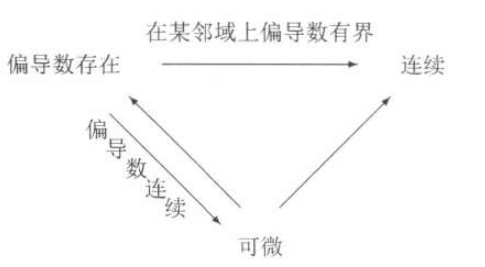
\includegraphics[width=\textwidth]{7.3.png} % 无需重复指定宽度  
\end{myimagebox}     
\caption{\label{fig:7.3}多元函数可微,偏导数和连续的关系}   
\end{figure}

\textbf{例}:设二元函数$f(x,y)$的解析式如下:
\begin{align*}
    f(x,y)=\begin{cases}
        xy\sin\frac{1}{x^2+y^2} &x^2+y^2\neq 0\\
        0 &x^2+y^2=0
        \end{cases}
\end{align*}

证明:(1)$f_x(0,0),f_y(0,0)$都存在。(2)$f_x(x,y),f_y(x,y)$在$(0,0)$处不连续。(3)函数$f(x,y)$在$(0,0)$连续。

\textbf{解:}(1)先计算当$(x,y)\neq(0,0)$时函数的偏导数:
\begin{align*}
&\frac{\partial f}{\partial x}=y\sin\frac{1}{x^2+y^2}-\frac{2x^2y}{(x^2+y^2)}\cos\frac{1}{x^2+y^2}\\
& \frac{\partial f}{\partial y}=x\sin\frac{1}{x^2+y^2}-\frac{2y^2x}{(x^2+y^2)}\cos\frac{1}{x^2+y^2}
\end{align*}

利用定义计算在$(0,0)$处的偏导数:
\begin{align*}
    f_x(0,0)=\frac{f(\Delta x,0)-f(0,0)}{\Delta x}=0\\
    f_x(0,0)=\frac{f(\Delta x,0)-f(0,0)}{\Delta x}=0
\end{align*}

(2)考虑从$y=x$和从$x$轴的趋近,在$(0,0)$处不存在极限,因此偏导数不连续。

(3)考虑当$\rho\to 0$时:
\begin{align*}
    |\frac{\Delta f-f_x\Delta x-f_y\Delta y}{\rho}|&=|\frac{\Delta x\Delta y}{\sqrt{(\Delta x)^2+(\Delta y)^2}}\sin\frac{1}{(\Delta x)^2+(\Delta y)^2}|\\
    &\leq\frac{(\Delta x)^2+(\Delta y)^2}{2\sqrt{(\Delta x)^2+(\Delta y)^2}}\to 0
\end{align*}

因此原函数可微。

\subsubsection{复合函数微分法与方向导数}
\begin{tcolorbox}[
    colback=bac1,     % 极浅黄色背景
    colframe=fra1,   % 浅黄色边框
    coltitle=white,             % 标题文字白色
    coltext=tex1,
    title=复合函数微分法,
    fonttitle=\bfseries,        % 标题加粗
arc=3mm,                     % 圆角稍大
breakable
]
设函数$u=\varphi(x,y),v=\psi(x,y)$在点$(x,y)$处关于$x,y$的偏导数存在,又设函数$z=f(u,v)$在相应的点$(u,v)$处关于$u,v$的偏导存在且连续,那么复合函数$z=f(\varphi(x,y),\psi(x,y))$在点$(x,y)$处的偏导数存在,且:
\begin{align*}
    \frac{\partial z}{\partial x}=\frac{\partial f}{\partial u}\frac{\partial u}{\partial x}+\frac{\partial f}{\partial v}\frac{\partial v}{\partial x}\\
     \frac{\partial z}{\partial y}=\frac{\partial f}{\partial u}\frac{\partial u}{\partial y}+\frac{\partial f}{\partial v}\frac{\partial v}{\partial y}\tag{7-7}
\end{align*}

这两个公式称作复合函数求导的\textbf{链式法则}。对其定理的证明不再赘述,从下图可以给出其的记忆方式:
\begin{figure}[H]    
\centering     
\renewcommand{\figurename}{图}     
\renewcommand{\thefigure}{7.4}    
\begin{myimagebox}[width=0.5\textwidth] % 直接传入图片尺寸参数      
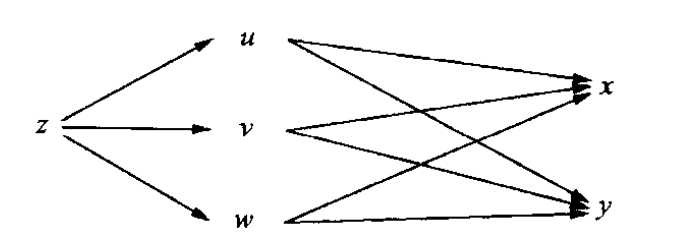
\includegraphics[width=\textwidth]{7.4.png} % 无需重复指定宽度  
\end{myimagebox}     
\caption{\label{fig:7.4}链式法则}   
\end{figure}
\end{tcolorbox}

\textbf{例}:设函数$z=f(x,y)$有连续的一阶偏导数,现做极坐标换元$x=r\cos\theta,y=r\sin\theta$,证明:
\begin{align*}
    z_r^2+\frac{1}{r^2}z_\theta^2=z_x^2+z_y^2
\end{align*}

\textbf{解}:直接套用链式法则:
\begin{align*}
    &z_r=z_x\cdot \cos\theta+z_y\cdot\sin\theta\\
    &z_\theta=z_x\cdot(-r\sin\theta)+z_y\cdot (r\cos\theta)
\end{align*}

然后直接带入即可。对于上述的链式法则我们可以做如下推广:
\begin{tcolorbox}[
    colback=bac1,     % 极浅黄色背景
    colframe=fra1,   % 浅黄色边框
    coltitle=white,             % 标题文字白色
    coltext=tex1,
    title=链式法则的推广,
    fonttitle=\bfseries,        % 标题加粗
arc=3mm,                     % 圆角稍大
breakable
]
设$z=f(u_1,u_2,...u_m)$可微,$u_i=g_i(x_1,x_2,...x_n)$有连续偏导,则:
\begin{align*}
(\frac{\partial z}{\partial x_1}, \frac{\partial z}{\partial x_2},...,\frac{\partial z}{\partial x_n})
=(\frac{\partial z}{\partial u_1},\frac{\partial z}{\partial u_2},...,\frac{\partial z}{\partial u_m})
\begin{pmatrix}
 \frac{\partial u_1}{\partial x_1} & \frac{\partial u_1}{\partial x_2} & ... & \frac{\partial u_1}{\partial x_n}\\
 \frac{\partial u_2}{\partial x_1}  &  \frac{\partial u_2}{\partial x_2} & ... &  \frac{\partial u_2}{\partial x_n}\\
 ... & ... & ... & ...\\
  \frac{\partial u_m}{\partial x_1} & \frac{\partial u_m}{\partial x_2} & ... &\frac{\partial u_m}{\partial x_n}
\end{pmatrix}  \tag{7-8}
\end{align*}
\end{tcolorbox}

一阶全微分具有形式不变性。无论$x,y$是中间变量还是自变量,全微分都可以表示成相同的形式。全微分的计算公式与之前介绍的办法相同,这里不再赘述。接下来我们需要考虑下面全微分的高阶微分:
\begin{align*}
    \mathrm{d}f=f_x(x,y)\mathrm{d}x+f_y(x,y)\mathrm{d}y
\end{align*}

我们考虑对其再进行一次微分,不难验证:
\begin{align*}
\mathrm{d}^2f=f_{xx}\mathrm{d}x^2+f_{xy}\mathrm{d}x\mathrm{d}y+f_{yx}\mathrm{d}y\mathrm{d}x+f_{yy}\mathrm{d}y^2
\end{align*}

如果二阶混合偏导数连续,那么就有$f_{xy}=f_{yx}$,就可以把中间两项合并,即就是:
\begin{align*}
    \mathrm{d}^2f=(\mathrm{d}x\frac{\partial }{\partial x}+\mathrm{d}y\frac{\partial}{\partial y})^2f
\end{align*}

因此我们假设$n$阶混合偏导都是连续的,那么高阶微分可以写作:
\begin{tcolorbox}[
    colback=bac1,     % 极浅黄色背景
    colframe=fra1,   % 浅黄色边框
    coltitle=white,             % 标题文字白色
    coltext=tex1,
    title=高阶微分,
    fonttitle=\bfseries,        % 标题加粗
arc=3mm,                     % 圆角稍大
breakable
]
高阶微分的形式为:
\begin{align*}
    \mathrm{d}^nf=(\mathrm{d}x\frac{\partial}{\partial x}+\mathrm{d}y\frac{\partial}{\partial y})^nf\tag{7-9}
\end{align*}
\end{tcolorbox}

接下来我们介绍方向导数和梯度。我们知道偏导数$f_x,f_y$是函数沿着相应坐标轴的变化率。那么函数沿着任意指定的一个方向的变化率该怎么计算?这需要引入\textbf{方向导数}的概念:
\begin{tcolorbox}[
    colback=bac2,     % 极浅黄色背景
    colframe=fra2,   % 浅黄色边框
    coltitle=white,             % 标题文字白色
    coltext=tex2,
    title=方向导数的定义,
    fonttitle=\bfseries,        % 标题加粗
arc=3mm,                     % 圆角稍大
breakable
]
设函数$z=f(x,y)$在点$P_0(x_0,y_0)$的一个邻域内有定义,又设$\bm{l}$是给定的一个方向,其方向余弦为$(\cos\alpha,\cos\beta)$。若极限:
\begin{align*}
    \lim_{t\to 0}\frac{f(x_0+t\cos\alpha,y_0+t\cos\beta)-f(x_0,y_0)}{t}
\end{align*}

存在,则称极限值为$z=f(x,y)$在点$P_0$处沿着$\bm{l}$方向的\textbf{方向导数}。记作$\frac{\partial z}{\partial\bm{l}}|_{(x_0,y_0)}$
\end{tcolorbox}

我们现在分析这个定义背后的含义。过点$P_0(x_0,y_0)$沿着方向$\bm{l}$做一条直线$L$,那么方向导数就是函数值在这条直线上的变化率。下面给出一个方向导数存在的充分条件和计算方法:
\begin{tcolorbox}[
    colback=bac1,     % 极浅黄色背景
    colframe=fra1,   % 浅黄色边框
    coltitle=white,             % 标题文字白色
    coltext=tex1,
    title=方向导数存在的充分条件与计算方式,
    fonttitle=\bfseries,        % 标题加粗
arc=3mm,                     % 圆角稍大
breakable
]
若函数$f(x,y)$在$P_0$处可微,则$f(x,y)$在该点沿着任意一个方向$\bm{l}$的方向导数均存在,并且:
\begin{align*}
    \frac{\partial  f}{\partial \bm{l}}|_{P_0}=f_x(x_0,y_0)\cos\alpha+f_y(x_0,y_0)\cos\beta\tag{7-10}
\end{align*}
\end{tcolorbox}

这个定理告诉我们,在函数可微的条件下,方向导数可以通过偏导数来计算。我们对这个定理进行证明:在方向$\bm{l}$上任取一点$P_t(x_0+t\cos\alpha,y_0+t\sin\alpha)$。因函数$f(x,y)$在点$(x_0,y_0)$可微,故该函数增量可表示为:
\begin{align*}
    f(P_t)-f(P_0)&=f(x_0+t\cos\alpha,y_0+t\cos\beta)-f(x_0,y_0)\\
    &=f_x(x_0,y_0)t\cos\alpha+f_y(x_0,y_0)t\cos\beta+o(\rho)
\end{align*}

其中$\rho$是$P_tP_0$的距离。两边同时除以$t$并去取极限,证毕。对于三元函数,方向梯度多一项$f_z\cos\gamma$即可。

\textbf{例}:求函数$f(x,y)=x^3y$在点$P_0(1,2)$处沿从点$P_0$到点$P(1+\sqrt{3},3)$的方向导数。

\textbf{解}:首先计算偏导数:$f_x=3x^2y=6,f_y=x^3=1$。然后计算方向余弦,得到$(\cos\alpha,\cos\beta)=(\frac{\sqrt{3}}{2},\frac{1}{2})$。因此方向导数为$3\sqrt{3}+\frac{1}{2}$。

方向导数告诉我们一个道理:函数沿着不同方向的变化率不同。那么到底沿着哪个方向函数变化率最大?我们对$7-10$进行变形:
\begin{align*}
    \frac{\partial f}{\partial \bm{l}}=(f_x,f_y)\cdot \bm{l_0}
\end{align*}

其中$\bm{l_0}$是方向$\bm{l}$的单位向量。那么本质上我们把7-10写成了一个向量的点乘。那么进一步来说,方向导数的最大值就是$\sqrt{f_x^2+f_y^2}$。因此我们把$(f_x(x_0,y_0),f_y(x_0,y_0))$称作函数$f(x,y)$在点$P$的梯度。记作:$\nabla f$。\textbf{函数的梯度是一个向量},\textbf{函数梯度的模长就是方向导数的最大值。当函数梯度与方向向量相反时,方向导数就是最小值}。梯度的计算规则如下:
\begin{align*}
    \nabla(u\pm v)=\nabla u\pm \nabla v \quad \nabla(uv)=v\nabla u+u\nabla v\quad \nabla(f(u,v))=f_u\nabla u+f_v\nabla v
\end{align*}

\subsection{多元函数的微分学公式与极值}
\subsubsection{微分中值定理和泰勒公式}
微分中值定理可以推广到多元函数。下面给出二元函数的拉格朗日中值定理:
\begin{tcolorbox}[
    colback=bac1,     % 极浅黄色背景
    colframe=fra1,   % 浅黄色边框
    coltitle=white,             % 标题文字白色
    coltext=tex1,
    title=二元函数拉格朗日中值定理,
    fonttitle=\bfseries,        % 标题加粗
arc=3mm,                     % 圆角稍大
breakable
]
设函数$z=f(x,y)$在区域$D$内有连续的一阶偏导数,又假定$D$中的两个点$P_0(x_0,y_0),P_1(x_0+\Delta x,y_0+\Delta y)$。并且$P_0P_1\subset D$,则存在$\theta\in(0,1)$使得:
\begin{align*}
    f(x_0+\Delta x,y_0+\Delta y)=f(x_0,y_0)+\frac{\partial f}{\partial x}(x_0+\theta \Delta x,y_0+\theta \Delta y)\Delta x+\frac{\partial f}{\partial y}(x_0+\theta\Delta x,y_0+\theta\Delta y)\Delta y\tag{7-11}
\end{align*}
\end{tcolorbox}

这个定理体现了,如果我们研究函数在某个方向上线段两侧函数值的变化量,其等于线段上某一点位置函数的全微分。我们接下来对此定理进行证明:考虑点$P_t(x_0+t\Delta x,y_0+t\Delta y)$,那么$\varphi(t)=f(P_t)$就是可微函数,因此对$t$求偏微分:
\begin{align*}
    \frac{\partial \varphi}{\partial t}=\frac{\partial f}{\partial x}x_0+ t\Delta x,y_0+t\Delta y)\Delta x+\frac{\partial f}{\partial y}(x_0+t\Delta x,y_0+t\Delta y)\Delta y
\end{align*}

而根据一元函数拉格朗日中值定理,存在$\theta\in(0,1)$使得$\varphi(1)-\varphi(0)=\varphi'(\theta)$,展开证毕。

\textbf{例}:设函数$z=f(x,y)$在区域$D$内有连续的一阶偏导数,且$f_x=f_y=0$在区域上恒成立。证明$z=f(x,y)$是常值函数。

\textbf{解:}在$D$内找一点$P_0(x_0,y_0)$,对于$D$内任意的点$P(x,y)$,若$PP_0$在区域内,就有:
\begin{align*}
    f(P)-f(P_0)=f_x(P_\theta)h+f_y(P_\theta)k=0
\end{align*}

若$PP_0$不在线段内,那么找折线$P_0P_1P_2...P_nP$即可。

类似于一元函数,二元函数也具有Taylor公式。想象一元函数Taylor展开的右侧是某一点的高阶导数,那么类比一下,在二元函数Taylor展开的右侧,应该是高阶全微分。而高阶全微分的形式我们在上一章有所讲解。因此我们得出二元函数的Taylor展开公式:
\begin{tcolorbox}[
    colback=bac1,     % 极浅黄色背景
    colframe=fra1,   % 浅黄色边框
    coltitle=white,             % 标题文字白色
    coltext=tex1,
    title=二元函数的Taylor展开,
    fonttitle=\bfseries,        % 标题加粗
arc=3mm,                     % 圆角稍大
breakable
]
设$D$是平面空间上的一个区域,$f(x,y)\in C^{n+1}(D)$,又设区域上存在两点$P_0(x_0,y_0)\in D,P_1(x_0+\Delta x,y_0+\Delta y)\in D,P_0P_1\subset D$,则有:
\begin{align*}
    f(x_0+\Delta x,y_0+\Delta y)=&f(x_0,y_0)+\frac{1}{1!}\mathrm{d}f(x_0,y_0)+\frac{1}{2!}\mathrm{d}^2f(x_0,y_0)+...\\
    +&\frac{1}{n!}\mathrm{d}^nf(x_0,y_0)+R_n(x_0,y_0)\tag{7-12}
\end{align*}

其中拉格朗日余项$R_n(x_0,y_0)$的解析式为:
\begin{align*}
    R_n(x)=\frac{1}{(n+1)!}\mathrm{d}^{n+1}(x_0+\theta\Delta x,y_0+\theta\Delta y)\tag{7-13}
\end{align*}
\end{tcolorbox}

证明过程类比于一元Taylor展开和二元Lagrange中值定理,这里不再赘述。对于拉格朗日余项,假设其$n+1$阶偏导数有界,那么我们就有:
\begin{align*}
    |R_n|\leq\frac{M}{(n+1)!}(|\Delta x|+|\Delta y)^{n+1}
\end{align*}

记$\rho=\sqrt{(\Delta x)^2+(\Delta y)^2}$,我们就能得到:
\begin{align*}
    |R_n|&\leq \frac{M\rho^{n+1}}{(n+1)!}(\frac{|\Delta x|}{\rho}+\frac{|\Delta y|}{\rho})^{n+1}\\
    &\leq \frac{2^{n+1}M}{(n+1)!}\rho^{n+1}
\end{align*}

因此当$\rho\to 0$时,$R_n=o(\rho^n)$。因此我们就可以得到带Pieno余项的Taylor公式。而前边的$n$项称作Taylor多项式。

\textbf{例}:计算函数$f(x,y)=\sin(\frac{\pi}{2}x^2y)$在$(1,1)$处的二阶泰勒多项式和带Pieno余项的Taylor公式。

\textbf{解:}第一步,计算高阶微分,这里面是二阶微分:
\begin{align*}
    \mathrm{d}^2f=f_{xx}(\Delta x)^2+f_{yy}(\Delta y)^2+f_{xy}\Delta x\Delta y
\end{align*}

第二步,计算所需要的高阶导数值:
\begin{align*}
    &f_x=\pi xy\cos(\frac{\pi}{2}x^2y)=0\qquad f_y=\frac{\pi}{2}x^2\cos(\frac{\pi}{2}x^2y)=0\\
    &f_{xx}=\pi y\cos(\frac{\pi}{2}x^2y)-\pi^2x^2y\sin(\frac{\pi}{2}x^2y)=-\pi^2\\
&f_{xy}= \pi x\cos(\frac{\pi}{2}x^2y)-\frac{\pi^2}{2}x^3\sin(\frac{\pi}{2}x^2y)=-\frac{\pi^2}{2}\\
&f_{yy}=-\frac{\pi^2}{4}x^4\sin(\frac{\pi}{2}x^2y)= -\frac{\pi^2}{4}\quad o(\rho)=\sqrt{(x-1)^2+(y-1)^2} 
\end{align*}

第三步,带入到Taylor展开式:
\begin{align*}
    \sin(\frac{\pi}{2}x^2y)=1-\frac{\pi^2}{2}[(x-1)^2+(x-1)(y-1)+\frac{1}{4}(y-1)^2]+o(\sqrt{(x-1)^2+(y-1)^2})
\end{align*}

同一元函数Taylor展开一样,多元函数也有Taylor展开的唯一性。
\begin{tcolorbox}[
    colback=bac2,     % 极浅黄色背景
    colframe=fra2,   % 浅黄色边框
    coltitle=white,             % 标题文字白色
    coltext=tex2,
    title=多元函数Taylor展开唯一性,
    fonttitle=\bfseries,        % 标题加粗
arc=3mm,                     % 圆角稍大
breakable
]
若$P_n(\Delta x,\Delta y)$是$\Delta x,\Delta y$的$n$次多项式,并且有$f(x_0+\Delta x,y_0+\Delta y)=P_n(\Delta x,\Delta y)+o(\rho^n)$

那么$P_n$就是Taylor多项式。
\end{tcolorbox}

\textbf{例}:利用Taylor展开唯一性,计算下面的两个函数在$(0,0)$的Taylor多项式,分别展开到二次项和四此项。
\begin{align*}
    (1)e^x\cos y\qquad (2) f(x,y)=\begin{cases}
        \frac{1-e^{x(x^2+y^2)}}{x^2+y^2} &(x,y)\neq (0,0)\\
        0 &(x,y)=(0,0)
    \end{cases}
\end{align*}

\textbf{解}:我们分别对$e^x,\cos y$做一元Taylor展开:
\begin{align*}
    e^x=1+x+\frac{1}{2}x^2+o(x^2)\qquad \cos y=1-\frac{1}{2}y^2+o(y)^2
\end{align*}

由于$o(x^2)\sim o(\rho^2),o(y^2)\sim o(\rho ^2)$,\textbf{将上面的式子相乘,保留$x^ny^m$系数之和不大于2的项}:
\begin{align*}
    T_n(x,y)=1+x+\frac{1}{2}x^2-\frac{1}{2}y^2
\end{align*}

(2)由于根据一元Taylor展开:
\begin{align*}
    e^{x(x^2+y^2)}=1+x(x^2+y^2)+\frac{1}{2}x^2(x^2+y^2)^2+o(\rho^4)
\end{align*}

因此:
\begin{align*}
    T_n(x)=\frac{  1-1-x(x^2+y^2)-x^2(x^2+y^2)^2+o(\rho^4)  }{x^2+y^2}=-x-\frac{1}{2}x(x^2+y^2)
\end{align*}

我们接下来进行一点小拓展,考虑用矩阵形式写出Taylor展开的表达式。考虑一个在$n$维空间子区域的$n$元二次连续可微函数$f(x_1,x_2,...x_n)$。设点$\bm{p}_0=(x_1^0,x_2^0,...x_n^0)$,那么带佩亚诺余项的二阶Taylor展开式为:
\begin{align*}
    f(\bm{p}_0+\Delta\bm{x})=f(\bm{p}_0)+\nabla f(\bm{p}_0)\cdot\Delta \bm{x}^T+\frac{1}{2!}\Delta\bm{x}\bm{Q}\bm{x}^T+o(r^2)\tag{7-14}
\end{align*}

最后我们再看多元Taylor公式的应用:

\textbf{例}:(1)令多元函数$u=\frac{x^2}{a^2}+\frac{y^2}{b^2}+\frac{z^2}{c^2},a>b>c>0$。求函数在$(0,0,0)$处增速最快的方向。

(2)设$g(x,y)=f(x,y)+2(x^2+y^2)$,在$D:x^2+y^2\leq 1$上有连续的一阶偏导。且$|f(x,y)|\leq 1$。证明存在$(x_0,y_0)$在$D$的内部,使得$f_x^2+f_y^2\leq 16$。

\textbf{解}:(1)我们的第一思路是计算在原点处的梯度,找原点处梯度的方向。但是在这一道题中原点处梯度为0,因此我们需要用其他办法。考察单位向量$\bm{l}=(\alpha,\beta,\gamma)$,计算下面的增量:
\begin{align*}
    \varphi(t)-\varphi(0)=u(t\alpha,t\beta,t\gamma)-u(0,0,0)
\end{align*}

对这个式子使用Taylor展开:
\begin{align*}
    \varphi(t)-\varphi(0)&=\varphi'(0)t+\frac{\varphi''(0)}{2}t^2+o(t^2)\\
    &=\frac{1}{2}(u_{xx}(0,0,0)\alpha^2+u_{yy}(0,0,0)\beta^2+u_{zz}(0,0,0)\gamma^2)t^2+o(t^2)\\
    &=(\frac{\alpha^2}{a^2}+\frac{\beta^2}{b^2}+\frac{\gamma^2}{c^2})t^2+o(t^2)
\end{align*}

由于$a>b>c,\alpha^2+\beta^2+\gamma^2=1$,因此$(0,0,\pm 1)$方向即为所求。

(2)在圆周上$g(x,y)\geq 1$,而在圆心处$g(x,y)\leq 1$。因此在$D$内一定有极小值,此时$g_x=g_y=0$,代入证毕。

\subsubsection{隐函数存在定理}
本章我们讨论的是:对于一个多元函数,其中一部分自变量是否可以表示成另一部分自变量的隐函数的问题。例如对于多元函数方程组:
\begin{align*}
    \begin{cases}
        F(x,y;u,v)=0\\
        G(x,y;u,v)=0
    \end{cases}
\end{align*}

其中$u,v$能否表示为$x,y$的函数?$u,v$是否可以计算对$x,y$的偏导数?本章我们研究的就是这样的问题。我们先冲一个最简单的情况入手,考虑函数$F(x,y)=0$中$y$是否可以写作$x$的隐函数:
\begin{tcolorbox}[
    colback=bac1,     % 极浅黄色背景
    colframe=fra1,   % 浅黄色边框
    coltitle=white,             % 标题文字白色
    coltext=tex1,
    title=隐函数存在定理(1方程,2未知数),
    fonttitle=\bfseries,        % 标题加粗
arc=3mm,                     % 圆角稍大
breakable
]
设函数$F(x,y)$在点$P_0(x_0,y_0)$的某个邻域内有定义,且满足$F(x_0,y_0)=0$,$F_x,F_y$连续且$F_y\neq 0$,则在$x_0$的某个邻域$(x_0-\delta,x_0+\delta)$内存在唯一的隐函数$y=f(x)$,使得:
\begin{align*}
    F(x,f(x))\equiv 0
\end{align*}

且$y=f(x)$有连续的导数,并且:
\begin{align*}
    f'(x)=-\frac{F_x(x,y)}{F_y(x,y)}\tag{7-14}
\end{align*}
\end{tcolorbox}

7-14式子的得来就是直接使用隐函数求导法即可,并没有新鲜之处。我们要注意,定理的结论是\textbf{局部性质},它并\textbf{没有告诉我们隐函数存在的邻域有多大},也就是说我们并不知道隐函数的定义域的情况。

\textbf{例}:对于函数
\begin{align*}
    f(x,y)=\frac{x^2}{a^2}+\frac{y^2}{b^2}-1\qquad a,b>0
\end{align*}

先证明其在$(\frac{a}{\sqrt{2}},\frac{b}{\sqrt{2}})$附近存在隐函数$y=f(x)$,再计算在这一点处隐函数的导数。

\textbf{解}:我们需要计算两个偏导数:
\begin{align*}
    F_x=\frac{2x}{a}=\frac{\sqrt{2}}{a}\qquad F_y=\frac{2y}{b}=\frac{\sqrt{2}}{b}
\end{align*}

显然偏导数都连续且$F_y\neq 0$。因此偏导数存在。另一方面,计算导数直接套用公式:
\begin{align*}
    y'(x)=-\frac{F_x}{F_y}=-\frac{b}{a}
\end{align*}

当然也可以利用隐函数求导法去计算,这两个方法本质上是一样的。我们接下来再看一道难度稍高的例题:

\textbf{例}:证明在$(1,1)$的某一邻域存在唯一连续可微函数$f(x)$,有$f(1)=1,xf(x)+2\ln x+3\ln f(x)-1=0$,并计算$f'(x)$。

\textbf{解}:我们构造下面的二元函数:
\begin{align*}
    F(x,y)=xy+2\ln x+3\ln y-1
\end{align*}

计算偏导数:
\begin{align*}
    F_x=y+\frac{2}{x}\qquad F_y=x+\frac{3}{y}
\end{align*}

这个偏导数连续,且$F_y(1,1)\neq 0$,因此$f(x)$的存在性证毕。直接套用公式计算隐函数的导数:
\begin{align*}
    f'(x)=-\frac{F_x}{F_y}=-\frac{xy^2+2y}{x^2y+3x}
\end{align*}

将上面的隐函数存在定理拓展到更多未知数,可以得到下面的结论:
\begin{tcolorbox}[
    colback=bac1,     % 极浅黄色背景
    colframe=fra1,   % 浅黄色边框
    coltitle=white,             % 标题文字白色
    coltext=tex1,
    title=隐函数存在定理(1方程,n+1未知数),
    fonttitle=\bfseries,        % 标题加粗
arc=3mm,                     % 圆角稍大
breakable
]
设函数$F(x_1,x_2,...x_n,y)$在点$P_0(x_1^0,x_2^0,...,x_n^0,y^0)$的某个邻域内有定义,且满足$F(P_0)=0$,$F_{x_j},F_y$连续$(j=1\sim n)$且$F_y\neq 0$,则在$P_0$的某个邻域内存在唯一的隐函数$y=f(x_1,x_2,...x_n)$,使得:
\begin{align*}
    F(x_1,x_2,...,x_n,f(x_1,x_2,...x_n))\equiv 0
\end{align*}

且$y=f(x_1,x_2,...x_n)$有连续的偏导数,并且:
\begin{align*}
    y_{x_j}=-\frac{F_{x_j}(x_1,x_2,...x_n,y)}{F_y(x_1,x_2,...,x_n,y)}\tag{7-15}
\end{align*}
\end{tcolorbox}

我们要注意,7-15的公式也是从隐函数求偏导法引申而来的结论,因此两种办法本质上是等价的。

\textbf{例}:(1)求由方程$F(x-y,y-z)=0$确定的隐函数$z=z(x,y)$的偏导数$z_x,z_y,z_{xy}$。

(2)设$z(x,y)$是方程$e^x\sin y+yz+e^z+5=0$所确认的隐函数,计算$z_x,z_{xy}$。

\textbf{解}:(1)我们假设$x-y,y-z$是变量$1,2$。函数对这两个变量直接求偏导是好计算的。接下来我们利用链式法则:
\begin{align*}
    F_1-z_xF_2=0\to z_x=\frac{F_1}{F_2}
\end{align*}

接下来对$y$求偏导,我们这里采用内直接套公式,当然也可以利用隐函数求导法:
\begin{align*}
    z_y=-\frac{F_y}{F_z}=\frac{-F_1+F_2}{-F_2}=\frac{F_2-F_1}{F_2}
\end{align*}

对于$z_{xy}$,我们对第一个式子两边对$y$求偏导:
\begin{align*}
    -F_{11}+F_{12}(1-z_y)-[-F_{21}+F_{22}(1-z_y)]z_x-F_2z_{xy}=0\\
-F_{11}+F_{12}\frac{F_1}{F_2}-(-F_{21}+F_{22}\frac{F_1}{F_2})\frac{F_1}{F_2}-F_2z_{xy}=0\\
z_{xy}=\frac{1}{F_2^3}(2F_1F_2F_{12}-F_2^2F_{11}-F_1^2F_{22})   
\end{align*}

(2)方程两边直接对$x$求偏导数:
\begin{align*}
    e^x\sin y+yz_x+e^zz_x&=0\\
    z_x&=\frac{-e^x\sin y}{y+e^z}
\end{align*}

然后再对$y$求偏导即可。

接下来我们考虑方程组的情况,我们先从最简单的2个方程,3个未知数入手:
\begin{align*}
    \begin{cases}
        F(x,u,v)=0\\
        G(x,u,v)=0
    \end{cases}
\end{align*}

我们考虑$u,v$对$x$的隐函数。那么有如下的定理:
\begin{tcolorbox}[
    colback=bac1,     % 极浅黄色背景
    colframe=fra1,   % 浅黄色边框
    coltitle=white,             % 标题文字白色
    coltext=tex1,
    title=隐函数存在定理(2方程,3未知数),
    fonttitle=\bfseries,        % 标题加粗
arc=3mm,                     % 圆角稍大
breakable
]
设函数$F(x,u,v),G(x,u,v)$在一点$(x_0,u_0,v_0)$的某个邻域内有连续的一阶偏导数,并且$F(x_0,u_0,v_0)=G(x_0,u_0,v_0)=0$,又设$F,G$关于$u,v$的\textbf{雅可比行列式}:
\begin{align*}
    J=\frac{D(F,G)}{D(u,v)}=\begin{vmatrix}
        F_u & F_v\\
        G_u & G_v
    \end{vmatrix}\neq 0\tag{7-16}
\end{align*}

那么在$x_0$的某个邻域内存在唯一的一对函数$u(x),v(x)$使得:
\begin{align*}
    \begin{cases}
        F(x,u(x),v(x))\equiv 0\\
        G(x,u(x),v(x))\equiv 0
    \end{cases}\tag{7-17}
\end{align*}

对7-17求偏导可以得到:
\begin{align*}
    \begin{cases}
        \frac{\partial F}{\partial x}+\frac{\partial F}{\partial u}\frac{\mathrm{d}u}{\mathrm{d}x}
+  \frac{\partial F}{\partial v}\frac{\mathrm{d}v}{\mathrm{d}x}=0\\
       \frac{\partial G}{\partial x}+\frac{\partial G}{\partial u}\frac{\mathrm{d}u}{\mathrm{d}x}
+  \frac{\partial G}{\partial v}\frac{\mathrm{d}v}{\mathrm{d}x}=0
    \end{cases}\tag{7-18} 
\end{align*}
\end{tcolorbox}

我们来看下面的一个例题:

\textbf{例}:设$u(x,y),v(x,y)$是下面的方程组所确定的隐函数,计算$u_x,u_{xx}$。
\begin{align*}
    \begin{cases}
        x=e^u+v\\
        xy=e^u+u
    \end{cases}
\end{align*}

\textbf{解}:对所给的方程中两端都对$x$取倒数,则有:
\begin{align*}
    1=e^u u_x+v_x\qquad y=e^uu_x+u_x
\end{align*}

解方程组之后得到$u_x=\frac{y}{e^u+1}$。然后对上面的方程组继续求导数:
\begin{align*}
    0=e^uu_x^2+e^uu_{xx}+u_{xx}
\end{align*}

解得:
\begin{align*}
    u_{xx}=\frac{-e^uy^2}{(e^u+1)^3}
\end{align*}

当然我们继续考虑一下隐函数存在的条件。计算Jacobbi行列式:
\begin{align*}
    J=\frac{D(F,G)}{D(u,v)}=e^u+1\neq 0
\end{align*}

因此隐函数在定义域上都存在。

\textbf{例}:设$u=f(x-ut,y-ut,z-ut),g(x,y,z)=0$,计算$u_x$,并且说明此时$t$是自变量还是因变量。

\textbf{解}:两个方程确定两个隐函数,一个是$u$,则另一个是$z$。因此$t$是自变量。两个方程都对$x$求导:

\begin{align*}
    \begin{cases}
        u_x=f_1(1-u_xt)-f_2u_xt+f_3(z_x-u_xt)\\
        g_1+g_3z_x=0
    \end{cases}
\end{align*}

解得:
\begin{align*}
    u_x=\frac{f_1-f_3\cdot\frac{g_1}{g_3}}{1+(f_1+f_2+f_3)t}
\end{align*}

最后我们介绍反函数组存在定理:
\begin{tcolorbox}[
    colback=bac1,     % 极浅黄色背景
    colframe=fra1,   % 浅黄色边框
    coltitle=white,             % 标题文字白色
    coltext=tex1,
    title=反函数组存在定理,
    fonttitle=\bfseries,        % 标题加粗
arc=3mm,                     % 圆角稍大
breakable
]
若函数$u=u(x,y),v=v(x,y)$在$(x_0,y_0)$某个邻域连续可微。且有:
\begin{align*}
    J=\frac{D(u,v)}{D(x,y)}\neq 0
\end{align*}

则在$(u_0,v_0)$的某一邻域存在唯一的反函数组$x=x(u,v),y=y(u,v)$满足$u_0=u(x_0,y_0),v_0=v(x_0,y_0)$且有:
\begin{align*}
    \frac{D(u,v)}{D(x,y)}\cdot\frac{D(x,y)}{D(u,v)}=1\tag{7-19}
\end{align*}
\end{tcolorbox}

例如我们常见的极坐标变换$x=r\cos\theta,y=r\sin\theta$。其中$r=\sqrt{x^2+y^2},\theta=\arctan\frac{y}{x}$。因此我们验证:
\begin{align*}
    \frac{D(x,y)}{D(r,\theta)}\cdot\frac{D(r,\theta)}{D(x,y)}=1
\end{align*}

最后我们补充隐函数存在定理在一般情况下的表达方式:
\begin{tcolorbox}[
    colback=bac1,     % 极浅黄色背景
    colframe=fra1,   % 浅黄色边框
    coltitle=white,             % 标题文字白色
    coltext=tex1,
    title=隐函数存在定理(m方程,m+n未知数),
    fonttitle=\bfseries,        % 标题加粗
arc=3mm,                     % 圆角稍大
breakable
]
设函数 \( \bm{F}(\bm{x}, \bm{u}) = \big(F_1(\bm{x}, \bm{u}), \dots, F_m(\bm{x}, \bm{u})\big) \) 在点 \( (\bm{x}_0, \bm{u}_0) \) 的某个邻域内有连续的一阶偏导数,其中:
\begin{itemize}
    \item \( \bm{x} = (x_1, \dots, x_n) \in \mathbb{R}^n \) 是自变量
    \item \( \bm{u} = (u_1, \dots, u_m) \in \mathbb{R}^m \) 是因变量
\end{itemize}
且满足:
\[
\bm{F}(\bm{x}_0, \bm{u}_0) = \bm{0},
\]
又设 \( \bm{F} \) 关于 \( \bm{u} \) 的雅可比行列式在$(\bm{x}_0, \bm{u}_0)$有:
\[
J = \frac{\partial(F_1, \dots, F_m)}{\partial(u_1, \dots, u_m)} = 
\begin{vmatrix}
\frac{\partial F_1}{\partial u_1} & \cdots & \frac{\partial F_1}{\partial u_m} \\
\vdots & \ddots & \vdots \\
\frac{\partial F_m}{\partial u_1} & \cdots & \frac{\partial F_m}{\partial u_m}
\end{vmatrix} \neq 0\tag{7-20} 
\]
那么在 \( \bm{x}_0 \) 的某个邻域内存在唯一的函数 \( \bm{u}(\bm{x}) = \big(u_1(\bm{x}), \dots, u_m(\bm{x})\big) \) 使得:
\[
\bm{F}\big(\bm{x}, \bm{u}(\bm{x})\big) \equiv \bm{0}.
\]
\end{tcolorbox}

\subsubsection{条件极值与拉格朗日乘子法}
在多元函数微分学的最后,我们介绍极值问题和最值问题。类似一元函数,我们首先需要对极值进行定义:
\begin{tcolorbox}[
    colback=bac2,     % 极浅黄色背景
    colframe=fra2,   % 浅黄色边框
    coltitle=white,             % 标题文字白色
    coltext=tex2,
    title=二元函数的极值,
    fonttitle=\bfseries,        % 标题加粗
arc=3mm,                     % 圆角稍大
breakable
]
设函数$f(x,y)$在区域$D$有定义,$(x_0,y_0)$是$D$的内点,若存在$(x_0,y_0)$的一个邻域,使得对该领域内任意一点$(x,y)$都有$f(x,y)\leq f(x_0,y_0)$,则称$f(x_0,y_0)$为函数的一个\textbf{极大值},$(x_0,y_0)$为函数的\textbf{极大值点}。
\end{tcolorbox}

与一元函数类似,我们也可以利用二元函数的偏导数来给出极值点存在的必要条件:若函数$f(x,y)$在点$(x_0,y_0)$处达到极值并且$f_x(x_0,y_0),f_y(x_0,y_0)$都存在,那么一定有:
\begin{align*}
    f_x(x_0,y_0)=f_y(x_0,y_0)=0\tag{7-21}
\end{align*}

我们称函数满足7-21的点为\textbf{稳定点},同一元函数类似,极值点一定是稳定点,但是稳定点不一定是极值点。在一元函数中我们利用二阶导数的情况判断是否为极值点,这里面对于二元函数是类似的。下面的定理证明比较繁琐,读者可自行看书:
\begin{tcolorbox}[
    colback=bac2,     % 极浅黄色背景
    colframe=fra2,   % 浅黄色边框
    coltitle=white,             % 标题文字白色
    coltext=tex2,
    title=二元函数的极值,
    fonttitle=\bfseries,        % 标题加粗
arc=3mm,                     % 圆角稍大
breakable
]
设函数$f(x,y)$在点$P_0(x_0,y_0)$的一个邻域内有连续的二阶偏导数,并且有:
\begin{align*}
    f_x(x_0,y_0)=f_y(x_0,y_0)=0
\end{align*}

我们令:
\begin{align*}
    A=f_{xx}(x_0,y_0)\quad B=f_{xy}(x_0,y_0)\quad C=f_{yy}(x_0,y_0)
\end{align*}

若$B^2<AC$,则$A>0$时为极小值点,$A<0$时为极大值点;$B^2>AC$时不是极值点。$B^2=AC$时不能确定。
\end{tcolorbox}

\textbf{例}:求函数$f(x,y)=x^4+y^4-x^2-2xy-y^2$的稳定点,并判别它们是否为极值点。

\textbf{解}:一阶偏导为0,因此:
\begin{align*}
    \begin{cases}
        f_x=4x^3-2x-2y=0\\
        f_y=4y^3-2x-2y=0
    \end{cases}
\end{align*}

因此解方程组,得到三个解为$(0,0),(1,1),(-1,-1)$。这三个点是稳定点。接下来我们判断极值点,根据原式有$f_{xx}=12x^2-2,f_{xy}=-2,f_{yy}=12y^2-2$。在$(1,1)$处$A=10,B=-2,C=10,B^2<AC$,因此是极小值点。在$(-1,-1)$处有$A=10,B=-2,C=10,B^2<AC$,因此$(-1,-1)$也是极小值点。在$(0,0)$处$A=B=C=-2$,因此无法判断。但是我们可以在$(0,0)$附近分析函数表达式。在直线$y=-x$上$f(x,-x)=2x^4>0$,而在$y=0$上$f(x,0)=x^4-x^2$,原点附近小于0,所以$(0,0)$不是极值点。

\begin{figure}[H]    
\centering     
\renewcommand{\figurename}{图}     
\renewcommand{\thefigure}{7.5}    
\begin{myimagebox}[width=0.5\textwidth] % 直接传入图片尺寸参数      
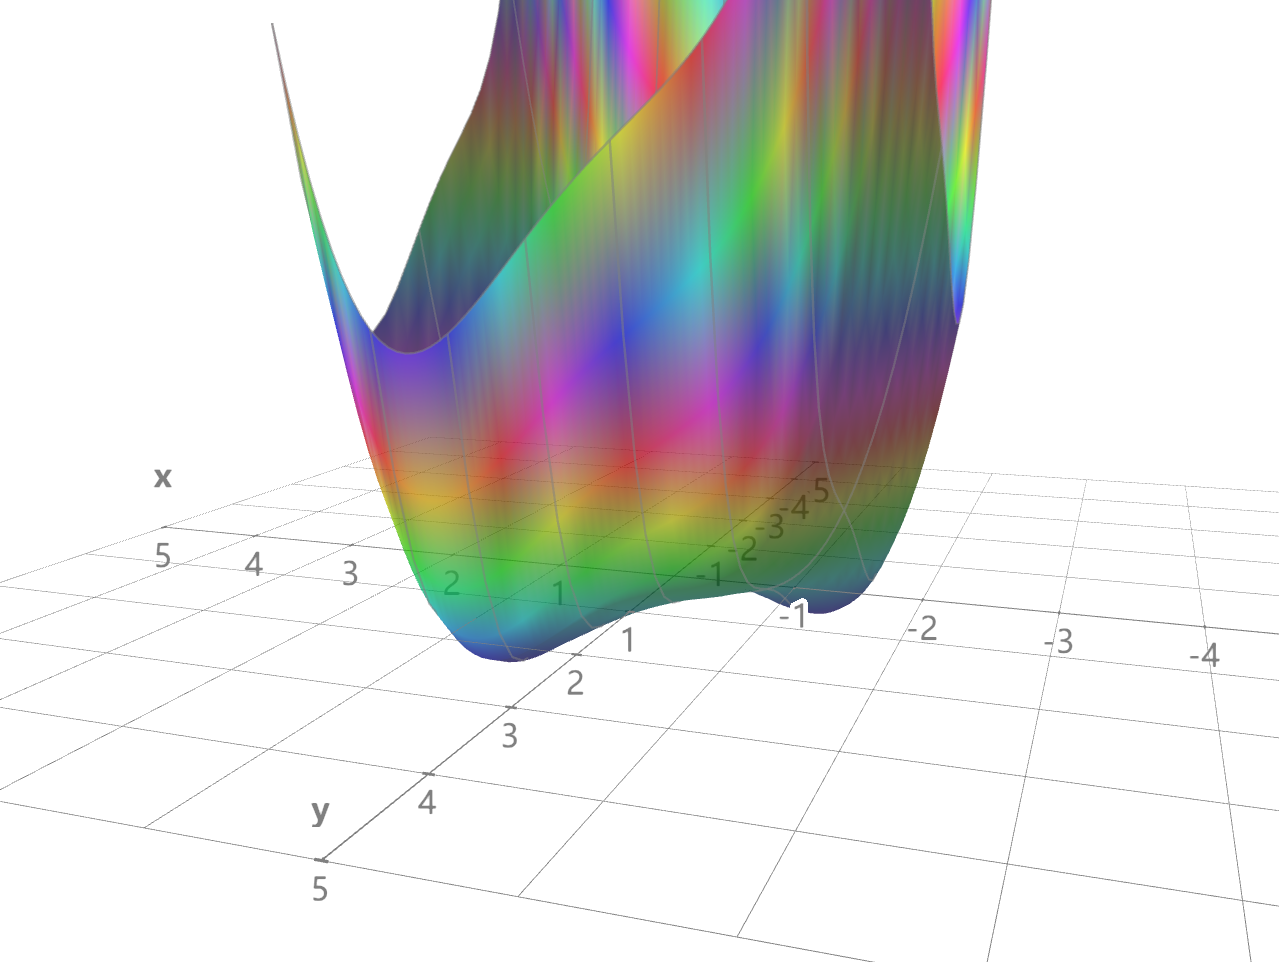
\includegraphics[width=\textwidth]{7.5.png} % 无需重复指定宽度  
\end{myimagebox}     
\caption{\label{fig:7.5}图象示意}   
\end{figure}

最后我们介绍\textbf{条件极值}问题。例如求函数$z=x^2+y^2$的极小值,显然是在原点取到。但是我们现在给它加一个限制条件:在$x+y=1$上取最小值,那这个问题就不一样了。我们考虑函数$z=f(x,y)$在$\varphi(x,y)=0$约束下的极值。假设$f(x,y),\varphi(x,y)$都有连续一阶偏导数$\varphi_y\neq 0$。那么我们找隐函数$y=y(x)$并且得到$z=f(x,y(x))$,那么这就变成了一个普通的极值问题。我们先求稳定点,有:
\begin{align*}
    \frac{\mathrm{d}z}{\mathrm{d}x}=f_x+f_yy'(x)=0
\end{align*}

根据隐函数求导公式,则有:
\begin{align*}
    f_x-f_y\frac{\varphi_x}{\varphi_y}=0\to \frac{f_x}{\varphi_x}=\frac{f_y}{\varphi_y}
\end{align*}

令其等于$-\lambda$,则引进辅助函数:
\begin{align*}
    F(x,y,\lambda)=f(x,y)+\lambda \varphi(x,y)
\end{align*}

那么上面的条件就是三元函数$F(x,y,\lambda)$普通极值点必须满足的条件。因此我们介绍下面的办法解决条件极值问题:

\begin{tcolorbox}[
    colback=bac1,     % 极浅黄色背景
    colframe=fra1,   % 浅黄色边框
    coltitle=white,             % 标题文字白色
    coltext=tex1,
    title=拉格朗日乘子法,
    fonttitle=\bfseries,        % 标题加粗
arc=3mm,                     % 圆角稍大
breakable
]
我们求函数$f(x_1,...x_n)$在约束条件:

$\varphi_1(x_1,...,x_n)=0$,$\varphi_2(x_1,...,x_n)=0$...$\varphi_k(x_1,x_2...,x_n)=0$下的极值,我们构造辅助函数:
\begin{align*}
F(x_1,...x_n,\lambda_1,...\lambda_k)=f(x_1,...,x_n)+\sum_{i=1}^k\lambda_i\varphi_i(x_1,...x_n)\tag{7-22}
\end{align*}

解方程组:
\begin{align*}
    \begin{cases}
        F_{x_1}=\frac{\partial f}{\partial x_1}+\lambda_1\frac{\partial \varphi_1}{\partial x_1}+
...+\lambda_k\frac{\partial \varphi_k}{\partial x_1}=0  \\
...\\
    F_{x_n}=\frac{\partial f}{\partial x_n}+\lambda_1\frac{\partial \varphi_1}{\partial x_n}+
...+\lambda_k\frac{\partial \varphi_k}{\partial x_n}=0 \\
F_{\lambda_1}=\varphi_1(x_1,x_2,...x_n)=0\\
F_{\lambda_k}=\varphi_k(x_1,x_2,...x_n)=0
    \end{cases}\tag{7-23}
\end{align*}

就可以得到约束条件下的稳定点。然后再根据一般二元函数的极值计算哪些是极大值点,哪些是极小值点。
\end{tcolorbox}

\textbf{例}:平面$x+y+z=1$截圆柱面$x^2+y^2=1$的截痕是一个椭圆周,求这个椭圆周离原点最近和最远的点。

\textbf{解}:到原点的距离为$z=\sqrt{x^2+y^2+z^2}$,约束条件为$x+y+z=1,x^2+y^2=1$。因此构造辅助函数:
\begin{align*}
    F(x,y,z,\lambda_1,\lambda_2)=x^2+y^2+z^2+\lambda_1(x+y+z-1)+\lambda_2(x^2+y^2-1)
\end{align*}

求解方程组:
\begin{align*}
    \begin{cases}
        F_x=2x+\lambda_1+2x\lambda_2=0\\
        F_y=2y+\lambda_1+2y\lambda_2=0\\
        F_z=2z+\lambda_1=0
    \end{cases}
\end{align*}

因此可以推出$x(1+\lambda_2)-z=0,y(1+\lambda_2-z)=0$。下面我们分类讨论:

如果$\lambda_2=-1$,那么可以推导$z=0$,然后根据约束条件得到$(1,0,0),(0,1,0)$两个稳定点。如果$\lambda_2\neq -1$,那么可以推导出$x=y$。计算后可有$(\frac{\sqrt{2}}{2},\frac{\sqrt{2}}{2},1-\sqrt{2}),(-\frac{\sqrt{2}}{2},-\frac{\sqrt{2}}{2},1+\sqrt{2})$两个点。然后最后判断四个稳定点的距离即可。

\subsection{习题补充与拓展}
本章的大部分习题和定理只需要基本掌握,内容考察的深度不算非常高,因此读者需好好掌握课本例题和往年考试题中出现的内容。

\textbf{例1}:设函数$f(x,y)$的解析式如下,判断函数在$(0,0)$点是否连续,是否可微。
\begin{align*}
    f(x,y)=\begin{cases}
        \frac{\sqrt{|x-y|}}{x^2+y^2}\sin(x^2+y^2) & (x,y)=(0,0)\\
        0 & (x,y)\neq (0,0)
    \end{cases}
\end{align*}

\textbf{解}:计算在$(0,0)$的极限:
\begin{align*}
    \lim_{(x,y)\to(0,0)}f(x,y)= \lim_{(x,y)\to(0,0)}\sqrt{|x-y|}\frac{\sin(x^2+y^2)}{x^2+y^2}
= \lim_{(x,y)\to(0,0)}\sqrt{|x-y|}=0
\end{align*}

因此是连续的。接下来考虑可微性,利用偏导数的定义:
\begin{align*}
f_x(0,0)=\lim_{\Delta x\to 0}\frac{f(\Delta x,0)-f(0,0)}{\Delta x}=\lim_{\Delta x\to 0}
\frac{\sqrt{|\Delta x|}\sin(\Delta x)^2}{(\Delta x)^3}  
\end{align*}

若$\Delta x>0$,这个极限是不存在的,因此不可微。

\textbf{例2}:设$f(x,y)$在区域$G:x^2+y^2<1$有定义,且$f(x,0)$在$x=0$处连续,$f_y(x,y)$在区域内有界,证明$f(x,y)$在原点处连续。

\textbf{解}:考虑:
\begin{align*}
    |f(\Delta x,\Delta y)-f(0,0)|\leq |f(\Delta x,\Delta y)-f(0,\Delta y)|+|f(0,\Delta y)-f(0,0)|
\end{align*}

第一部分由于$f(x,0)$在$x=0$处连续,则极限为0;第二部分考虑$|f_y(x,y)|\leq M$,因此小于$M\Delta y$,趋近于0,因此不等式右侧趋近于0,证毕。

\textbf{例3}:设$x=x(u,v),y=y(u,v)$满足
\begin{align*}
    \frac{\partial x}{\partial u}=\frac{\partial y}{\partial v}\qquad \frac{\partial x}{\partial v}=-\frac{\partial y}{\partial u}
\end{align*}


且$w=w(x,y)$满足:
\begin{align*}
    \frac{\partial ^2 w}{\partial x^2}+    \frac{\partial ^2 w}{\partial y^2}=0
\end{align*}

证明:
\begin{align*}
    \frac{\partial ^2 w}{\partial u^2}+    \frac{\partial ^2 w}{\partial v^2}=0
\end{align*}

\textbf{解}:直接计算偏微分。
\begin{align*}
w_u&=w_xx_u+w_yy_u\\
w_{uu}&=w_{xx}x_u^2+w_xx_{uu}+w_{yy}y_u^2+w_yy_{uu}\\
w_v&=w_xx_v+w_yy_v\\
w_{vv}&=w_{xx}x_v^2+w_xx_{vv}+w_{yy}y_v^2+w_yy_{vv}
\end{align*}

直接相加后代入条件即可。

\textbf{例4}:(1)设$y=y(x)$由下面的方程决定,计算$y',y''$。
\begin{align*}
    xy-2^x\ln 2+2^y=0
\end{align*}

(2)设$z=z(x,y)$由下面的方程决定,求$z_{xx}$(读者可自己求$z_{yy},z_{xy}$)。
\begin{align*}
    f(x+y,y+z,z+x)=0
\end{align*}

\textbf{解}:(1)直接套公式即可:
\begin{align*}
    y'=-\frac{F_x}{F_y}=\frac{2^x(\ln 2)^2-y}{x+2^y\ln 2}
\end{align*}

然后对函数左右两侧继续求导,化简得到:
\begin{align*}
    y''=\frac{1}{x+2^y\ln 2}\left[2^x(\ln 2)^3-\frac{2^x(\ln 2)^2-y}{x+2^y\ln 2}(2+2^x\ln^22)\right]
\end{align*}

(2)不妨令$u=x+y,v=y+z,w=z+x$,两边对$x$求导:
\begin{align*}
    f_u+f_uz_x+f_w(z_x+1)=0\to z_x=-\frac{f_u+f_w}{f_v+f_w}
\end{align*}

两边对$x$求导之后展开:
\begin{align*}
    f_{xx}=-\frac{[f_{uu}+f_{ww}(z_x+1)](f_v+f_w)+[f_{vv}z_x+f_{ww}(z_x+1)](f_u+f_v)}{(f_v+f_w)^2}
\end{align*}

\textbf{例5}:求由$x=u\cos v,y=u\sin v,z=v$确定的隐函数$z=z(x,y)$所有的二阶偏导。

\textbf{解}:由题目条件可得:
\begin{align*}
\begin{cases}
\mathrm{d}x=\cos v\mathrm{d}u-u\sin v\mathrm{d}v\\
\mathrm{d}y=\sin v\mathrm{d}u+u\cos v\mathrm{d}v     
\end{cases}
\end{align*}

然后解方程可以得到:
\begin{align*}
\begin{cases}
\mathrm{d}u=\cos v\mathrm{d}x+u\sin v\mathrm{d}y\\
u\mathrm{d}v=-\sin v\mathrm{d}x+u\cos v\mathrm{d}y     
\end{cases}
\end{align*}

对第二个式子进行微分:
\begin{align*}
u\mathrm{d}v^2+\mathrm{d}v\mathrm{d}u=-\cos v\mathrm{d}v\mathrm{d}x-\sin v\mathrm{d}v\mathrm{d}y
=-\mathrm{d}u\mathrm{d}v   
\end{align*}

解得:
\begin{align*}
\mathrm{d}z^2&=\mathrm{d}v^2=-\frac{2}{u}\mathrm{d}u\mathrm{d}v\\
    &=-\frac{2}{u^2}(\cos v\mathrm{d}x+\sin v\mathrm{d}y)(-\sin v\mathrm{d}x+\cos v\mathrm{d}y)\\
&=\frac{2}{u^2}(\sin v\cos v\mathrm{d}x^2-\cos 2v\mathrm{d}x\mathrm{d}y-\sin v\cos v\mathrm{d}y^2)        
\end{align*}

因此我们有:
\begin{align*}
\mathrm{d}z^2&=\mathrm{d}v^2=-\frac{2}{u}\mathrm{d}u\mathrm{d}v\\
    &=-\frac{2}{u^2}(\cos v\mathrm{d}x+\sin v\mathrm{d}y)(-\sin v\mathrm{d}x+\cos v\mathrm{d}y)\\
&=\frac{2}{u^2}(\sin v\cos v\mathrm{d}x^2-\cos 2v\mathrm{d}x\mathrm{d}y-\sin v\cos v\mathrm{d}y^2)        
\end{align*}

因此可以直接判断二阶导数。注意$u_{xy}$的系数要除2。

\textbf{例6}:(1)设$f(x,y)$在点$(0,1)$附近无穷次可微,且$f_y(0,1)=0,f(0,1)=0$。证明$f(x,\int_0^t \sin x\mathrm{d}x)=0$在$(0,\frac{\pi}{2})$附近可确定隐函数$t=\varphi(x)$,求$\varphi'(0)$。

(2)设$f(x,y)$在点$P_0(x_0,y_0)$可微,$\bm{l_1},\bm{l_2}...\bm{l_n}$为$n$哥单位向量且相邻的两个夹角为$\frac{2\pi}{n}$。证明:
\begin{align*}
    \sum_{i=1}^n\frac{\partial f}{\partial\bm{l_i}}(x_0,y_0)=0
\end{align*}

\textbf{解}:(1)不妨令:
\begin{align*}
    F(x,t)=f(x,\int_0^t\sin x\mathrm{d}x)=f(x,1-\cos t)
\end{align*}

那么在$(0,\frac{\pi}{2})$对$x,t$有连续偏导。并且$(0,\frac{\pi}{2})$处$f(0,1)=0,f_y(0,1)\neq 0$。因此:
\begin{align*}
    \varphi'(0)=-\frac{F_x}{F_t}=-\frac{f_x(0,1)}{f_y(0,1)}
\end{align*}

(2)由于:
\begin{align*}
\frac{\partial f}{\partial\bm{l_i}}(x_0,y_0)=f_x(P_0)\cos\frac{2\pi i}{n}+f_y(P_0)\sin\frac{2\pi i}{n}          
\end{align*}

而$\sum_{i=1}^n\frac{\cos 2\pi i}{n}= \sum_{i=1}^n\frac{\sin 2\pi i}{n}=0$。证毕。

\textbf{例7}:求$f(x,y)=\sin x\sin y\sin(x+y)$在区域$D:\{(x,y)|x\geq 0,y\geq 0,x+y\leq \pi\}$上的极大值和极小值。

\textbf{解}:我们现寻找稳定点:
\begin{align*}
\begin{cases}
f_x=\sin y\sin(2x+y)=0\\
f_y=\sin x\sin(x+2y)=0
\end{cases}
\end{align*}

然后在区域内寻找解有$P_1(0,0),P_2(0,\pi),P_3(\pi,0),P_4(\pi,\pi),P_5(\frac{\pi}{3},\frac{\pi}{3}),P_6(\frac{2\pi}{3},\frac{\pi}{3})$。由于$P_1\sim P_4$在边界上,因此不是极值点。我们进一步计算参数:
\begin{align*}
    A=f_{xx}=2\sin y\cos(2x+y)\quad B=f_{xy}=\sin(2x+2y)\quad C=f_{yy}=2\sin x\cos(x+2y)
\end{align*}

在$P_5$处,$A<0,\Delta>0$,因此计算的是极大值$\frac{3\sqrt{3}}{8}$;在$P_6$处,,$A>0,\Delta>0$,因此计算的是极小值$-\frac{3\sqrt{3}}{8}$
\end{document}